\documentclass[11pt,letterpaper,twoside]{report}
% layout
\usepackage{geometry}
\usepackage{indentfirst}
\usepackage{setspace}
\usepackage{titlesec}
\usepackage[subfigure]{tocloft}

% citations
\usepackage{natbib}
\usepackage{apalike}
%\usepackage{etoolbox}
%\apptocmd{\sloppy}{\hbadness 10000\relax}{}{}

% include citations inline
\usepackage{bibentry}
\nobibliography*

% table
\usepackage{threeparttable}
\usepackage{multirow}

% figures
\usepackage{graphicx}
\usepackage{booktabs}
\usepackage{multicol}
\usepackage{listings}
\usepackage{subfig}
\usepackage{overpic}


% algorithm
\usepackage{algorithm}
%\usepackage{algpseudocode}
\usepackage{algorithmic}

% math
\usepackage{amsthm}
\usepackage{amsmath}
\usepackage{amssymb}
\usepackage{units}
\usepackage{array}

% typography
\usepackage{times}
\usepackage{microtype}
\usepackage{textcomp}

% macro support
\usepackage{xspace}
\usepackage[table]{xcolor}
\usepackage{pdflscape}
\usepackage{rotating}


% page floats
\usepackage{afterpage}

% pdf links
%\usepackage[hidelinks]{hyperref}

% use proper margins.
\geometry{letterpaper,left=1.25in,top=1in,right=1.25in,bottom=1in,nohead}

% double-space text
\doublespacing

% color
\usepackage{color}

% Center chapter titles, omit page numbers.
\titleformat{\chapter}[display]{\fillast\bfseries}{\Large\MakeUppercase{\chaptertitlename} \thechapter}{-11pt}{\huge\singlespacing}[\thispagestyle{empty}]

% extend to 2in top margins, leave 22pts = 2x font size after heading
\titlespacing{\chapter}{0in}{0.62in}{22pt}

% indent paragraphs four spaces throughout the thesis/dissertation.
\setlength{\parindent}{4ex}

% tweak spacing of paragraph labels.
\titlespacing{\paragraph}{0in}{0.08in}{0.07in}

% we want numbered subsubsections
\setcounter{secnumdepth}{3}
\setcounter{tocdepth}{3}

% we need to double-space between footnotes.
\setlength{\footnotesep}{13pt}

% we don't want crazy vertical spacing.
\raggedbottom

% we don't want abandoned words.
\clubpenalty=10000 
\widowpenalty=10000

% cite with (name, year)
\renewcommand{\cite}{\citep}

% common abbreviations
\newcommand{\eg}{{\it e.g.}\xspace}
\newcommand{\ie}{{\it i.e.}\xspace}
\newcommand{\etc}{{\it etc.}\xspace}
\newcommand{\etal}{\emph{et~al}\mbox{.}\xspace}

\newcommand{\xth}{\ensuremath{^{\text{th}}}\xspace}
%\newcommand{\fst}{\ensuremath{^{\text{st}}}\xspace}

% common math notation
\newcommand{\NAT}[0]{\mathbb{N}\xspace}
\newcommand{\fun}[1]{\mathit{#1}} % typeset as function name
\newcommand{\setsize}[1]{\left| #1 \right|}
\newcommand{\setdef}[2]{\left\{ #1 \ \left|\  #2\right.\right\}}
\newcommand{\dispsum}[0]{\displaystyle\sum}

\newcommand{\defeq}[0]{\triangleq}
\renewcommand{\mod}{\operatorname{mod}}

% time units
\newcommand{\mus}[0]{\ensuremath{\mu s}\xspace}
\newcommand{\us}[0]{\ensuremath{\mu s}}
\newcommand{\ms}[0]{\ensuremath{\fun{ms}}\xspace}

% algorithm names
\newcommand{\kwfont}[1]{\textsf{#1}\xspace} %\small
% variable name
\newcommand{\var}[1]{\ensuremath{{\fun{#1}}}\xspace} %\small

%http://hstuart.dk/2007/08/03/programming-latex-%E2%80%94-writing-commands/
\newcommand{\mkkw}[2]{\newcommand{#1}[0]{\kwfont{#2}}}

% fancy symbols and functions
\newcommand{\Alg}[0]{{\mathcal A}}
\newcommand{\Test}[0]{{\mathcal T}}
\newcommand{\Mach}[0]{{\mathcal M}}

\newcommand{\usum}[0]{u_{\mathrm{sum}}}
\newcommand{\umax}[0]{u_{\mathrm{max}}}
\newcommand{\umin}[0]{u_{\mathrm{min}}}
\newcommand{\utop}[0]{u_{\mathrm{top}}}

\newcommand{\esum}[0]{e_{\mathrm{sum}}}
\newcommand{\emax}[0]{e_{\mathrm{max}}}
\newcommand{\emin}[0]{e_{\mathrm{min}}}
\newcommand{\etop}[0]{e_{\mathrm{top}}}

\newcommand{\dsum}[0]{\delta_{\mathrm{sum}}}
\newcommand{\dmax}[0]{\delta_{\mathrm{max}}}
\newcommand{\dmin}[0]{\delta_{\mathrm{min}}}
\newcommand{\dtop}[0]{\delta_{\mathrm{top}}}

\newcommand{\prio}[0]{\mathsf Y}
\newcommand{\eprio}[0]{\mathsf y}

\newcommand{\Tr}{\operatorname{Tr}}

\newcommand{\TODO}[1]{\textbf{\textcolor{red}{[TODO: #1]}}}

% src code
\newcommand{\src}[1]{\textsf{\small #1}\xspace}

% references
\newcommand{\chref}[1]{Chapter~\ref{ch:#1}\xspace}
\newcommand{\chrefs}[2]{Chapters~\ref{ch:#1} and~\ref{ch:#2}\xspace}
\newcommand{\secref}[1]{Section~\ref{sec:#1}\xspace}
\newcommand{\figref}[1]{Figure~\ref{fig:#1}\xspace}
\newcommand{\figrefi}[2]{Figure~\ref{fig:#1}(#2)\xspace}
\newcommand{\tabref}[1]{Table~\ref{tab:#1}\xspace}
\newcommand{\lemref}[1]{Lemma~\ref{lem:#1}\xspace}
\newcommand{\thmref}[1]{Theorem~\ref{thm:#1}\xspace}
\newcommand{\defref}[1]{Definition~\ref{def:#1}\xspace}
\newcommand{\exref}[1]{Example~\ref{ex:#1}\xspace}
\newcommand{\equref}[1]{Equation~(\ref{eq:#1})\xspace}
\newcommand{\inequref}[1]{Inequality~(\ref{eq:#1})\xspace}
\newcommand{\lstref}[1]{Listing~\ref{lst:#1}\xspace}
\newcommand{\pref}[1]{page~\pageref{p:#1}\xspace}





% special footnotes
% from http://help-csli.stanford.edu/tex/latex-footnotes.shtml
\long\def\symbolfootnote[#1]#2{\begingroup%
\def\thefootnote{\fnsymbol{footnote}}\footnote[#1]{#2}\endgroup}

% theorems, etc.
\newtheoremstyle{mylemthm}% hnamei 
        {6pt}% hSpace abovei 
        {3pt}% hSpace belowi 
        {\slshape}% hBody fonti 
        {}% hIndent amounti1
        {\bfseries}% hTheorem head fonti 
        {.}% hPunctuation after theorem headi 
        {.5em}% hSpace after theorem headi2
        {}% hTheorem head spec (can be left empty, meaning `normal')i

\theoremstyle{mylemthm}
\newtheorem{theorem}{Theorem}[chapter]
\newtheorem{lemma}{Lemma}[chapter]

\newtheoremstyle{mydef}% hnamei 
        {3pt}% hSpace abovei 
        {3pt}% hSpace belowi 
        {\normalfont}% hBody fonti 
        {}% hIndent amounti1
        {\bfseries}% hTheorem head fonti 
        {.}% hPunctuation after theorem headi 
        {.5em}% hSpace after theorem headi2
        {\thmname{#1} \thmnumber{#2}\thmnote{#3}}% hTheorem head spec (can be left empty, meaning `normal')i
\theoremstyle{mydef}

%% Flush words right at end of paragraph.
%% From: http://tex.stackexchange.com/questions/16330/hfill-after-linebreak
\newcommand\rightparend[1]{{%
      \unskip\nobreak\hfil\penalty50
      \hskip2em\hbox{}\nobreak\hfil\textbf{#1}%
      \parfillskip=0pt \finalhyphendemerits=0 \par}}

\newtheorem{definition}{Definition}[chapter]
\newtheorem{xxexample}{Example}[chapter]

\makeatletter
\renewcommand{\maketag@@@}[1]{\hbox{\m@th\normalsize\normalfont#1}}%
\makeatother

%% "inherent" from xxexample, but place box at the end of example.
\newenvironment{example}{
\begin{xxexample}
}{
\rightparend{$\Diamond$}
\end{xxexample}
}
% \qed   \sqbullet \blackdiamond \vartriangleleft

\graphicspath{{figures/}}














\newcommand{\trace}{\operatorname{Tr}}
\newcommand{\vectorize}{\operatorname{vec}}
\newcommand{\sign}{\operatorname{sgn}}
\newcommand{\cdf}{\operatorname{cdf}}
\newcommand{\argmax}{\operatorname{argmax}}




\newcommand{\Cfree}{\ensuremath{\mathcal C_{\text{free}}}}
\newcommand{\Cobs}{\ensuremath{\mathcal C_{\text{obs}}}}
\newcommand{\Cspace}{\ensuremath{\mathcal C\text{-space}}}
\newcommand{\Ccont}{\ensuremath{\mathcal C_\text{cont}}}
\newcommand{\vol}{\operatorname{Vol}}

\newcommand{\Rn}{\ensuremath{\mathbb R^n}}
\newcommand{\Rsqr}{\ensuremath{\mathbb R^2}}
\newcommand{\Rcubic}{\ensuremath{\mathbb R^3}}
\newcommand{\SEcubic}{\ensuremath{\mathbb {SE}(3)}}
\newcommand{\SOcubic}{\ensuremath{\mathbb {SO}(3)}}
\newcommand{\SEsqr}{\ensuremath{\mathbb {SE}(2)}}
\newcommand{\q}{\ensuremath{\mathbf q}}
\newcommand{\x}{\ensuremath{\mathbf x}}
\newcommand{\knn}{\ensuremath{k\text{-NN}}}


\newcommand{\LCS}{\ensuremath{LCS}}
\newcommand{\LCSa}{\ensuremath{LCS_0}}
\newcommand{\LCSb}{\ensuremath{LCS_1}}
\newcommand{\LCSi}{\ensuremath{LCS_i}}
\newcommand{\LCSiplus}{\ensuremath{LCS_{i+1}}}


\newcommand{\qv}{\ensuremath{\mathbf q_v}}
\newcommand{\qc}{\ensuremath{\mathbf q_c}}
\newcommand{\qs}{\ensuremath{\mathbf q_s}}
\newcommand{\qa}{\ensuremath{\mathbf q_0}}

\newcommand{\dist}{\operatorname{dist}}
\newcommand{\argmin}{\operatorname{argmin}}
\newcommand{\PDt}{\ensuremath{PD_t}}
\newcommand{\PDg}{\ensuremath{PD_g}}

\newcommand{\V}{\ensuremath{V}}
\newcommand{\SV}{\ensuremath{S}}
\newcommand{\SVLCSa}{\ensuremath{S_{LCS_0}}}
\newcommand{\SVLCS}{\ensuremath{S_{LCS}}}

\DeclareMathOperator{\isLeaf}{isLeaf}
\DeclareMathOperator{\exactIntersect}{exactIntersect}
\DeclareMathOperator{\overlap}{overlap}
\DeclareMathOperator{\pop}{pop}

\newcommand{\erf}{\operatornamewithlimits{cdf}}
\newcommand{\diag}{\operatornamewithlimits{diag}}

\renewcommand{\ttdefault}{lmtt}


\newenvironment{remark}[1][Remark]{\begin{trivlist}
\item[\hskip \labelsep {\bfseries #1}]}{\end{trivlist}}



\begin{document}

%******************
% frontmatter pages use two inch top margin
\newgeometry{left=1.25in,top=2in,right=1.25in,bottom=1in,nohead}
\pagenumbering{roman}

%title page
\begin{titlepage}
\begin{center}
% 1. The title of the thesis/dissertation, centered 2” below the top of the page
\vspace{2in}
\begin{singlespace}
\Large \bf
Efficient Configuration Space Construction and Optimization
%CLOSED-LOOP PLANNING AND CONTROL \\OF STEERABLE MEDICAL NEEDLES
\end{singlespace}

% 2. Your name, centered 1” below the title.
\vspace{61pt} % 1 in = 72pt, 11pt for the line with text
\large Jia Pan
\end{center}


%3. The following statement, within the full mar- gins, 1” below your name:
%“A dissertation [or thesis] submitted to the faculty of the University of North Carolina at Chapel Hill in partial fulfillment of the requirements for the degree of	in the Department [or School or Curriculum] of      .”
\vspace{50pt}
\begin{singlespace}
\noindent \large
A dissertation submitted to the faculty of the University of North Carolina at Chapel Hill
in partial fulfillment of the requirements for the degree of Doctor of Philosophy in
the Department of Computer Science.
\end{singlespace}

%4. On the lower half of the page, centered, the words “Chapel Hill”
%and one line below that, the year in which your committee approves
%the completed thesis/dissertation.
\vspace{50pt}
\begin{center}
\begin{singlespace} \large
Chapel Hill\\
2013
\end{singlespace}
\end{center}

%5. On the right-hand side of the page, “Approved by,” followed by lines for the
%signatures of the adviser and four (two for thesis) readers. List

\vfill
\begin{flushright}
\begin{minipage}[t]{1.5in} \large
Approved by:\\
%To be approved by: \\
Dinesh Manocha \\
Ming C. Lin \\
Ron Alterovitz \\
Jan-Michael Frahm \\
Sachin Chitta
\end{minipage}
\end{flushright}
\end{titlepage}


% copyright page (optional)
\newgeometry{left=1.25in,top=8.33in,right=1.25in,bottom=1in,nohead}
%If you wish to copyright your thesis, you must include a copyright page with the following information single-spaced and centered on the bottom half of the page:
%(C) Year 
%Full Name (exactly as it appears on the title page) 
%ALL RIGHTS RESERVED
%This page should immediately follow the title page, and should bear the lower case Roman numeral: ii.
\begin{center}
\begin{singlespace}
\copyright 2013\\
Jia Pan \\
ALL RIGHTS RESERVED
\end{singlespace}
\end{center}

\vspace{2in}


% normal pages from here on out
\restoregeometry

% abstract
%The word “Abstract” should be centered 2? below the top of the page. 
%Skip one line, then center your name followed by the title of the 
%thesis/dissertation. Use as many lines as necessary. Centered below the 
%title include the phrase, in parentheses, “(Under the direction of  
%_________)” and include the name(s) of the dissertation advisor(s).
%Skip one line and begin the content of the abstract. It should be 
%double-spaced and conform to margin guidelines. An abstract should not 
%exceed 150 words for a thesis and 350 words for a dissertation. The 
%latter is a requirement of both the Graduate School and UMI's 
%Dissertation Abstracts International.
%Because your dissertation abstract will be published, please prepare and 
%proofread it carefully. Print all symbols and foreign words clearly and 
%accurately to avoid errors or delays. Make sure that the title given at 
%the top of the abstract has the same wording as the title shown on your 
%title page. Avoid mathematical formulas, diagrams, and other 
%illustrative materials, and only offer the briefest possible description 
%of your thesis/dissertation and a concise summary of its conclusions. Do 
%not include lengthy explanations and opinions.
%The abstract should bear the lower case Roman number ii (if you did not 
%include a copyright page) or iii (if you include a copyright page).
\begin{center}
\vspace*{52pt}
{\Large \textbf{ABSTRACT}}
\vspace{11pt}
\begin{singlespace}
JIA PAN: Efficient Configuration Space Construction and Optimization\\
(Under the direction of Dinesh Manocha)
\end{singlespace}
\end{center}

The configuration space is an important concept widely used in algorithmic robotics. Many applications in robotics, computer-aided design, and related areas can be reduced to computational problems in terms of configuration spaces. In this dissertation, we address three main computational challenges related to configuration spaces: 1) how to efficiently compute an approximate representation of high-dimensional configuration spaces; 2) how to efficiently perform geometric, proximity, and motion planning queries in high-dimensional configuration spaces; and 3) how to model uncertainty in configuration spaces represented by noisy sensor data.


We present new configuration space construction algorithms based on machine learning and geometric approximation techniques. These algorithms perform collision queries on many configuration samples. The collision query results
are used as input to compute an approximate representation for the configuration space, which quickly converges to the exact configuration space. We highlight the efficiency of our algorithms for penetration depth computation and
instance-based motion planning. We also present parallel GPU-based algorithms to accelerate the performance of optimization and search computations in configuration spaces. In particular, we design efficient GPU-based parallel $k$-nearest neighbor and parallel collision detection algorithms and use these algorithms
to accelerate motion planning. In order to extend configuration space algorithms to handle noisy sensor data arising from real-world robotics applications,
we model the uncertainty in the configuration space by formulating the collision probabilities for noisy data.
We use these algorithms to perform reliable motion planning for the PR2 robot.



%% dedication, acknowledgements and/or preface (all optional)
%A dedication is an honorific statement from the author to a person or group to 
%whom the author commends the effort and product of the dissertation. Most 
%dedications are short statements of tribute beginning with “To…”. No heading is 
%required on the dedication page. The text of short dedications should be 
%centered between the left and right margins and 2? from the top of the page.
\begin{center}
\vspace*{52pt}
To Inspector Gadget.
\end{center}

%Acknowledgements are the author's statement of gratitude to and
%recognition of the people and institutions who helped the author's
%research and writing.
\begin{center}
\vspace*{52pt}
{\Large \textbf{ACKNOWLEDGEMENTS}}
\end{center}

There are many people who through support, kindness, and constructive criticism have contributed a great deal to my research in graduate school and this thesis. First and foremost, I would like to thank my advisor Dinesh Manocha, who has been a constant source of guidance throughout my time here.  Dinesh has consistently pushed me to accomplish as much as possible during my time in the department. I have also benefited greatly from my committee members, for their support and suggestions on how to improve this dissertation.

I would additionally like to thank Liangjun Zhang, both for his cheerful mentorship and for introducing me to robotics -- which would forever change my research career. I have also been blessed with a large supply of collaborators in the GAMMA research group. In addition, I would like to give special thanks to Sandy Huang for her thorough and creative proofreading of this dissertation.

I would also like to thank my parents, who have always done everything possible to support my education and nurture my development.

%\begin{center}
\vspace*{52pt}
{\Large \textbf{PREFACE}}
\end{center}

Lorem ipsum dolor sit amet, consectetur adipiscing elit. Fusce sed vehicula felis. Etiam nisi mauris, malesuada et pulvinar vitae, vehicula eu mauris. Vivamus orci quam, euismod vel porta at, mollis quis ipsum. Donec a enim libero, vitae fringilla est. Sed varius nisl pulvinar lectus ultricies dictum. Curabitur mattis suscipit eros, suscipit vulputate erat blandit et. Suspendisse in neque ac ante volutpat ornare a et augue. Aliquam erat volutpat. Pellentesque aliquet congue enim, non convallis leo imperdiet sed. Quisque eget luctus ipsum. Proin lorem felis, molestie sit amet scelerisque at, ultrices a elit. Aenean placerat enim sed ante convallis quis vulputate orci bibendum. Duis sit amet accumsan magna. Sed adipiscing enim non elit pellentesque euismod.

%
%% table of contents, with page references
\renewcommand{\contentsname}{TABLE OF CONTENTS}
\renewcommand{\cfttoctitlefont}{\hfill\bfseries}
\renewcommand{\cftaftertoctitle}{\hfill}
\renewcommand{\cftdotsep}{1.5}
\cftsetrmarg{1.0in}

\setlength{\cftbeforetoctitleskip}{61pt}
\setlength{\cftaftertoctitleskip}{28pt}

% format chapter entries like other entries
\renewcommand{\cftchapfont}{\normalfont}
\renewcommand{\cftchappagefont}{\normalfont}
\renewcommand{\cftchapleader}{\cftdotfill{\cftdotsep}}

\newlength\mylen
\renewcommand\cftchappresnum{CHAPTER }
\settowidth\mylen{\cftchappresnum\cftchapaftersnum}
\addtolength\cftchapnumwidth{\mylen}
\renewcommand\cftchapaftersnum{:}




\setlength{\cftbeforechapskip}{15pt}
\setlength{\cftbeforesecskip}{10pt}
\setlength{\cftbeforesubsecskip}{10pt}
\setlength{\cftbeforesubsubsecskip}{10pt}

\begin{singlespace}
\tableofcontents
\end{singlespace}


%% list of tables, with titles and page references (if applicable)
\renewcommand{\listtablename}{LIST OF TABLES}
\phantomsection
\addcontentsline{toc}{chapter}{LIST OF TABLES}
\setlength{\cftbeforelottitleskip}{-11pt}
\setlength{\cftafterlottitleskip}{22pt}
\renewcommand{\cftlottitlefont}{\hfill\bfseries}
\renewcommand{\cftafterlottitle}{\hfill}
\setlength{\cftbeforetabskip}{10pt}
\begin{singlespace}
\listoftables
\end{singlespace}


%% list of figures or illustrations, with titles and page references (if applicable)
\renewcommand{\listfigurename}{LIST OF FIGURES}
\phantomsection
\addcontentsline{toc}{chapter}{LIST OF FIGURES}
\setlength{\cftbeforeloftitleskip}{-11pt}
\setlength{\cftafterloftitleskip}{22pt}
\renewcommand{\cftloftitlefont}{\hfill\bfseries}
\renewcommand{\cftafterloftitle}{\hfill}
\setlength{\cftbeforefigskip}{10pt}
\cftsetrmarg{1.0in}
\begin{singlespace}
\listoffigures
\end{singlespace}


%% list of abbreviations (if applicable)
%\phantomsection
\addcontentsline{toc}{chapter}{LIST OF ABBREVIATIONS}
\begin{center}
{\Large \textbf{LIST OF ABBREVIATIONS}}
\end{center}
\newcommand{\Ab}[2]{\noindent  #1 \> #2 \\}
\newcommand{\Abi}[2]{\noindent #1 \hspace{1.5cm} \= #2 \\}
\begin{tabbing}
\Abi{ABD}{All But Dissertation}
\Ab{I/O}{Input/Output}
\Ab{IPC}{Inter-Process Communication}
\Ab{IPI}{Inter-Processor Interrupt}
\Ab{WSS}{Working Set Size}
\Ab{AYO}{Add Your Own in alphabetic order\ldots}
\end{tabbing}


% list of symbols (if applicable)
%\phantomsection
\addcontentsline{toc}{chapter}{LIST OF SYMBOLS}
\begin{center}
{\Large \textbf{LIST OF SYMBOLS}}
\end{center}

%******************

% mainmatter
\pagenumbering{arabic}

% a chapter
%\chapter{Introduction}
\label{chp:intro}
Intelligent robots are becoming increasingly important in both industry and everyday life. In industry, rising labor costs are motivating manufacturers to consider using more robots in factories. For example, the average minimum wage in China has increased by more than 20 percent in 2012, while the supply of manufacturing robots has also increased by 51 percent in China~\cite{IFR:report}. 
Europe and USA exhibit similar trends: Intelligent robots are being designed in order to make workers more productive and make manufacturers more competitive in terms of price and quality. One recent example among these intelligent robots is the new ``Baxter'' robot~\cite{Brooks:2012:Baxter}, which is equipped with software that enables the robot to learn various tasks from human demonstration, recognize different objects, and react intelligently to external forces. Intelligent robots are expected to assist people in everyday life. In the future, such robots are expected to perform various tasks, including 1) household and care support, such as cooking and laundry; 2) healthy life support, such as chatting with the elderly and taking care of people with disabilities; and 3) labor support in unsafe working conditions such as chemical plants~\cite{Yamazaki:2012}. Several successful prototypes for assistant robots exist. For example, the PR2 robot from Willow Garage has been shown to assist people with severe physical disabilities such as quadriplegia~\cite{PR2HumanityWeb}; humanoid robots such as the HRP-4 can perform human-like actions and can communicate with people using speech~\cite{HRP-Cyber}. In addition to their applications in industry and everyday life, modern intelligent robots can be helpful in other areas, including autonomous vehicles~\cite{Montemerlo:2008:JSE}, medical and surgical intervention ~\cite{Bonfe:2012}, emergency and disaster rescue~\cite{Fukushima:2011}, and military tasks~\cite{AlphaDog:2012}.



\begin{figure}[!htb]
  \centering
  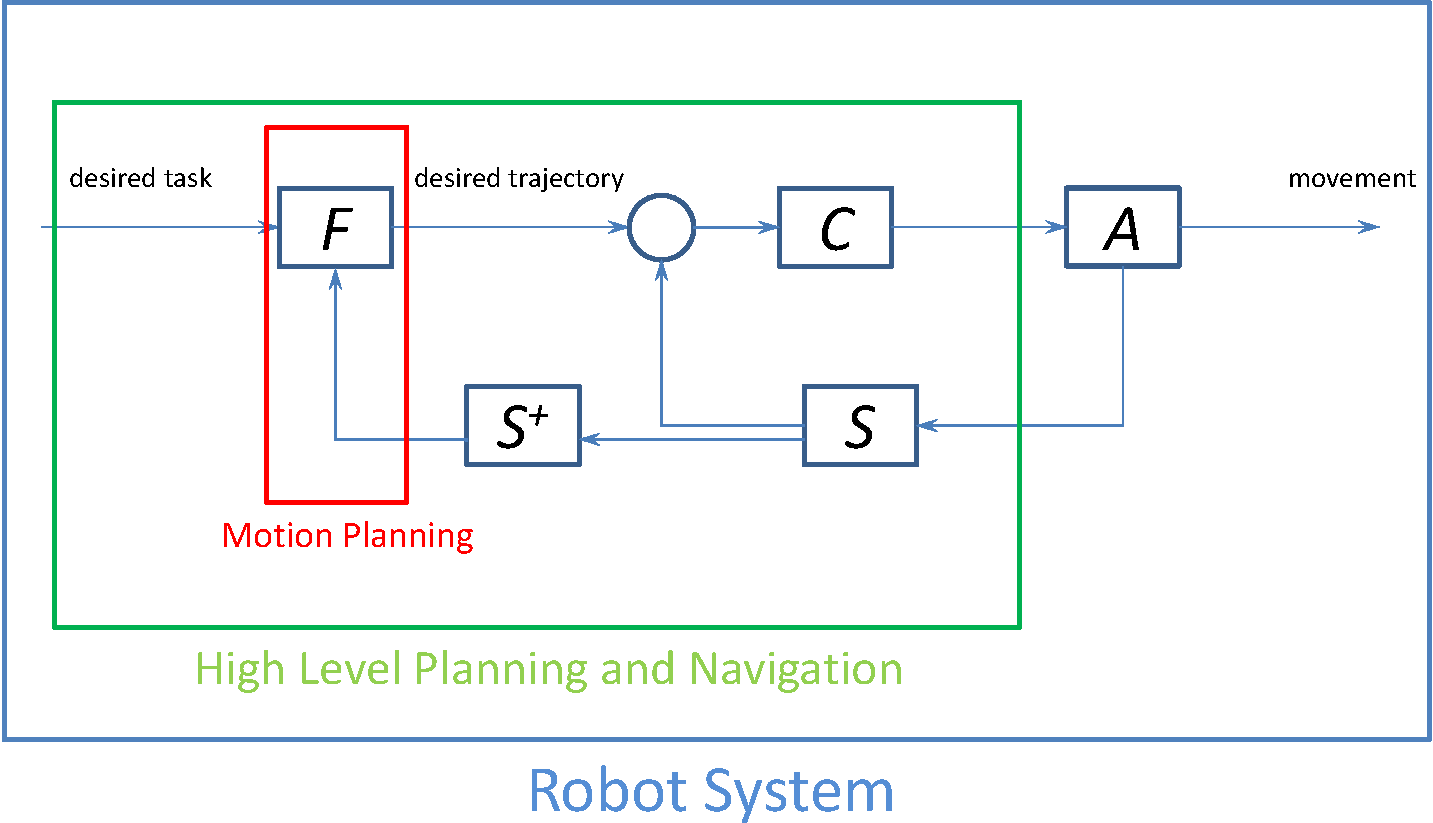
\includegraphics[width=\linewidth]{figs/1/pipeline-crop.pdf}
  \caption[Important hardware and software subsystems in a robot system]{Important hardware and software subsystems in a robot system. 1) Feed-forward system (F), including task planning, navigation strategy, motion planning and trajectory generation. 2) Control system (C), including kinematics, dynamics and control algorithms. 3) Actuator system (A), including motors, servos, transmissions, and so forth. 4) Sensor system (S), including various sensors such as camera, laser, IMU and related low level sensor data processing algorithms such as signal processing, estimation and fusion. 5) Sensor post-processing system (S$^+$), including localization, mapping, etc. The main software component of a robot system is the \emph{high level planning and navigation}, which determines the instructions sent to the actuator system, given the desired tasks to be executed. One important component of high level planning and navigation is \emph{motion planning}, which focuses on computing the trajectory from the environment description.}
  \label{fig:1:pipeline}
\end{figure}

The tremendous improvement in the design and availability of intelligent robots over the last decade is based on progress in many related areas, including computer vision, artificial intelligence, machine learning, control, sensor systems, and mechanical systems, which correspond to different components of an intelligent robot system (Figure~\ref{fig:1:pipeline}). For example, the SLAM (simultaneous localization and mapping) algorithm enables a robot to accurately track its position in an unknown environment~\cite{PR:2005}. In addition, with the help of advanced vision techniques, robots can now recognize and segment objects from background point clouds~\cite{Rusu:2009:IROS}. 
Compared to traditional industrial robots, one important feature of the modern intelligent robot system is \emph{high level planning and navigation}. Its main purpose is to compute low-level instructions based on high level descriptions for the tasks to be executed; these low-level instructions are then provided to the robot actuator system.
This planning and navigation component is composed of many different sub-components (Figure~\ref{fig:1:pipeline}) and there has been extensive work in this area, such as task planning~\cite{LPT:TPP:1989}, feedback from observation~\cite{KLP:2012:UPE,KLP:2011:NOW}, optimal control~\cite{Stengel:1994:OC}, and adaptive control~\cite{Astrom:1994:AC}.


One of the most important sub-systems of the high level planning and navigation component is the \emph{motion planning} system, which enables the robot to move safely from an initial position to a goal position without colliding with any static or moving obstacles in the environment. Motion planning enables robots to work efficiently and reliably in dynamic environments along with humans. Motion planning problems can be directly formalized and solved in the 3D workspace, for instance with the widely-used potential field algorithms~\cite{Khatib:IJRR:1986}. However, these workspace solutions cannot easily handle robots with different geometries and mechanical constraints. To overcome these difficulties, 
motion planning may be formalized and solved in a new space called the \emph{configuration space}~\cite{Lozano-Perez:1979:APC,LPT:APM:1981,LPT:SpatialPlanning:1983}. In the configuration space, a robot with a complex geometric shape in 3D workspace is mapped to a point robot and the robot's trajectory corresponds to a continuous curve in the high-dimensional configuration space (Figure~\ref{fig:1:planning}). Based on the configuration space formulation, the motion planning problem can be solved in two steps:

\begin{enumerate}
\item Construct a representation of the configuration space.
\item Perform optimization based on the computed representation.
\end{enumerate}

This motion planning pipeline based on configuration spaces is very successful and is adopted by many real-world planning applications that require optimal planning solutions. Many different representations for the configuration space have been proposed, including polyhedrons~\cite{Chazelle:ADS:1987}, semi-algebraic sets~\cite{Canny:1988:AGC,Canny:1988:CKP}, graphs~\cite{Kavraki96}, and trees/forests~\cite{Kuffner00}. Different optimization approaches have been proposed for different configuration space representations, including computing a shortest path, computing the minimum distance to the boundary of a closed set inside the configuration space, and so forth. Moreover, the same pipeline is also implicitly used in some motion planning algorithms for only computing a feasible path (i.e., a collision-free path that does not violate other constraints). For example, many variants of Rapidly Exploring Random Tree (RRT)~\cite{Kuffner00} use different heuristics to guide the search toward the goal configuration while growing a search tree structure as an approximate representation of the configuration space. Such a strategy can be viewed as a variant of the above pipeline, in which the configuration space construction alternates with the optimization computation.


However, this algorithmic pipeline based on $\Cspace$ still has many computational challenges:
\begin{enumerate}
\item Efficiently compute an approximate or exact representation for the configuration space is difficult, especially for high-DOF robots with high-dimensional configuration spaces. Such configuration space approximation problem would have exponential complexity (Section~\ref{sec:1:configconstruction}).
\item Many robotics applications require real-time planning in order to work reliably and efficiently in human environments with moving obstacles, but performing optimization in the computed representation for the configuration space can be time consuming (Section~\ref{sec:1:optimization}).
\item A robot in the real world depends on various sensors to acquire knowledge about its own state and the surrounding environments. Since the sensors provide noisy data, one important open problem involves enhancing the configuration space to consider robots and environments with noisy geometries. In contrast, previous work on configuration space based computations assume an exact representation of the robot and obstacles (Section~\ref{sec:1:uncertainty}).
\end{enumerate}


\section{Configuration Space}
\label{sec:1:configurationSpace}
The configuration space is a key concept used in classical mechanics to describe and analyze the motion of many important systems~\cite{Arnold:1989}. Generally, a \emph{configuration} $\q$ is a vector of independent parameters uniquely specifying the state of a system; a configuration space or $\Cspace$ is a collection of all possible configurations for a given system. For example, for a system of $n$ point particles, the configuration is a vector describing the positions of all the particles and the corresponding $\Cspace$ is $\mathbb R^{3n}$; the configuration of a 3D rigid body consists of its position and orientation, and the configuration space is $\SEcubic$ if both rotation and translation are allowed, and $\Rcubic$ if only translation is allowed; the configuration of an articulated object is the vector of all its joint angles.

The configuration space of a robot $A$ is composed of two components: \emph{collision-free space} $\Cfree = \{\q: A(\q) \cap B = \emptyset\}$ and \emph{in-collision space} or \emph{obstacle space} $\Cobs = \{\q: A(\q) \cap B \neq \emptyset\}$, where $B$ corresponds to the geometric representation of obstacles in the environment and $A(\q)$ corresponds to $A$ with the configuration $\q$. $\Cobs$ is a closed set and its boundary is denoted as the \emph{contact space} $\Ccont = \partial \Cobs$, which corresponds to the set of configurations where $A$ and $B$ just touch each other without penetration. Figure~\ref{fig:1:contactspace} shows an example of the $\Cspace$ of two objects where $\Ccont$ is highlighted with an orange curve.

\begin{figure}[!htb]
  \centering
  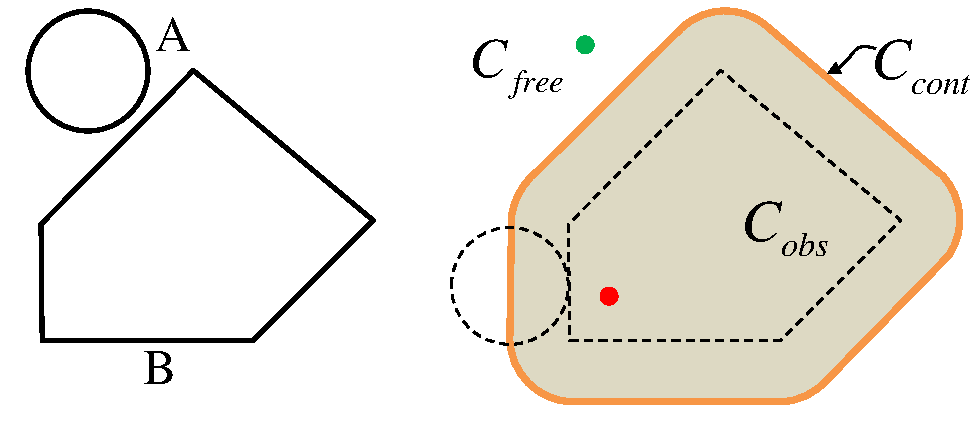
\includegraphics[width=0.6\linewidth]{figs/1/Ccont.pdf}
  \caption[The configuration space of two objects]{The configuration space of two objects. The orange curve highlights the contact space $\Ccont$ of $A$ and $B$. A point inside/on the orange curve belongs to
  $\Cobs$ and a point outside the orange curve belongs to $\Cfree$.
  The red and green points denote configurations in $\Cobs$ and $\Cfree$, respectively. Intuitively, $\Ccont$ is the boundary that separates in-collision and collision-free configurations.}
  \label{fig:1:contactspace}
\end{figure}

In the special case when $A$ and $B$ are both rigid objects and robot $A$ can only perform translation motion, $\Cobs$ is equal to the well-known Minkowski sum between $A$ and $B$: $\Cobs = A \oplus (-B) = \{\x = \x_A + \x_B | \x_A \in A, \x_B \in -B \}$. One example of the Minkowski sum is shown in Figure~\ref{fig:1:contactspace}. When robot $A$ can perform general motion (i.e., both translation and rotation), the geometry of $\Cobs$ is much more complicated, as shown by the 2D example in Figure~\ref{fig:1:cspaceSE2}.

\begin{figure}[!htb]
  \centering
  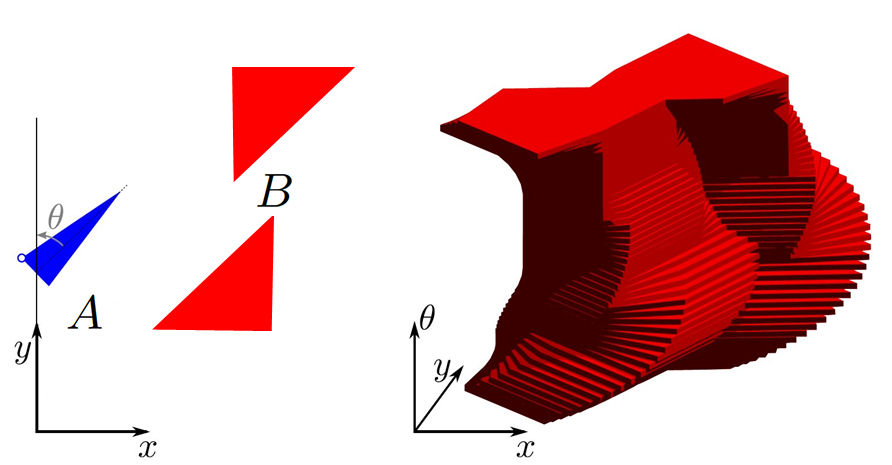
\includegraphics[width=0.9\linewidth]{figs/1/cspaceSE2.png}
  \caption[$\Cobs$ between 2D rigid objects $A$ and $B$]{$\Cobs$ between 2D rigid objects $A$ and $B$. For each rotation angle $\theta \in [0, 2\pi)$, we can compute the Minkowski sum between $A(\theta)$ and $-B$, where $A(\theta)$ is the resulting shape after rotating $A$ about the origin with $\theta$ degrees. When stacking the Minkowski sums for all angles $\theta$, we obtain the $\Cobs$ between $A$ and $B$. This figure is modified from an online image with unknown source.}
  \label{fig:1:cspaceSE2}
\end{figure}

Based on the notion of configuration space, the motion planning problem in 3D workspace can be reduced to path planning for a point robot in $\Cspace$, i.e., finding a curve in $\Cfree$ connecting the given initial and goal configurations of the robot.

\section{Configuration Space Construction}
\label{sec:1:configconstruction}
Before performing the motion planning computation in the configuration space, one prerequisite is to compute the geometry of $\Cspace$ in an appropriate representation (e.g., a graph or a surface). Since $\Cspace = \Cfree \cup \Cobs$ and $\Cfree \cap \Cobs = \emptyset$, we only need to construct the representation for either $\Cfree$ or $\Cobs$. Another equivalent solution is to compute $\Ccont$, the boundary between $\Cfree$ and $\Cobs$.

Previous work on configuration space construction can be categorized into two different methods: geometry-based and topology-based. Geometry-based methods compute the exact geometric representation of the configuration space while topology-based methods capture the connectivity of the configuration space.

Geometry-based methods are usually limited to low-dimensional configuration spaces, due to the combinatorial complexity involved in computing the boundary of $\Cobs$ for high-dimensional configuration spaces. Most previous work has focused on the special case when objects $A$ and $B$ are rigid bodies only performing translational motion. As mentioned in Section~\ref{sec:1:configurationSpace}, the resulting $\Cobs$ is the Minkowski sum between $A$ and $-B$. Even for this special case, the computational complexity involved in computing $\Cobs$ is still high: the complexity is $\mathcal O(mn)$ when $A$ and $B$ are both convex-objects and is $\mathcal O(m^3n^3)$ when $A$ and $B$ are both non-convex objects~\cite{Halperin:2002:RGC}, where $m$ and $n$ are the number of triangles in $A$ and $B$, respectively. In addition to the high complexity, most existing implementations for computing the Minkowski sum are prone to challenges that arise in the context of 3D geometric algorithms. In particular, these implementations are 1) not robust to numerical errors, and 2) susceptible to degeneracies (i.e., cannot reliably handle polygon soups or meshes with holes). Recent work has proposed methods~\cite{Lien:2008:CMS,Lien:2007:ACD,Lien:2009:ASM} for computing the approximate Minkowski sum efficiently and reliably, but these methods are also prone to robustness issues and can have high complexity in terms of dealing with complex objects. Options other than the Minkowski sum exist for computing  $\Cobs$. For example, Varadhan et al. compute the $\Cobs$ for 2D objects with rotation and translation by approximating the $\Cobs$ with an adaptive grid~\cite{Varadhan:2006:TPA}; Zhang et al. compute an approximation to 4D $\Cspace$ using cell decomposition~\cite{Zhang:2007:IROS}.

Topology-based methods capture the connectivity of the configuration space. Most previous approaches attempt to capture the connectivity of $\Cfree$ using sampling techniques~\cite{Kavraki96,Kuffner00}. The basic idea is first to generate random samples (called milestones) in $\Cfree$ and then organize these samples using a graph structure or a forest of tree structures (Figure~\ref{fig:1:topologycspace}). As the topology of $\Cfree$ can be rather complex, and
may consist of multiple components or small, narrow passages, it is hard to capture the full connectivity of $\Cfree$ using random sampling. There is extensive work on improving the connectivity computation by using different sampling strategies~\cite{Amato:1998:OOP,Boor:1999:ICRA,Hsu:1998:FNP,Rodriguez:2006,Zhang:2008:ICRA,Zheng:2005}. Recent work attempts to capture the topology of both $\Cfree$ and $\Cobs$~\cite{Jory:2011:IROS}. Topology-based methods can compute an approximate $\Cspace$ representation much faster than geometry-based methods. However, these methods do not work well with narrow passages and can be slow for high-DOF robots.


\begin{figure}[!htb]
  \centering
  \subfloat[Graph representation]{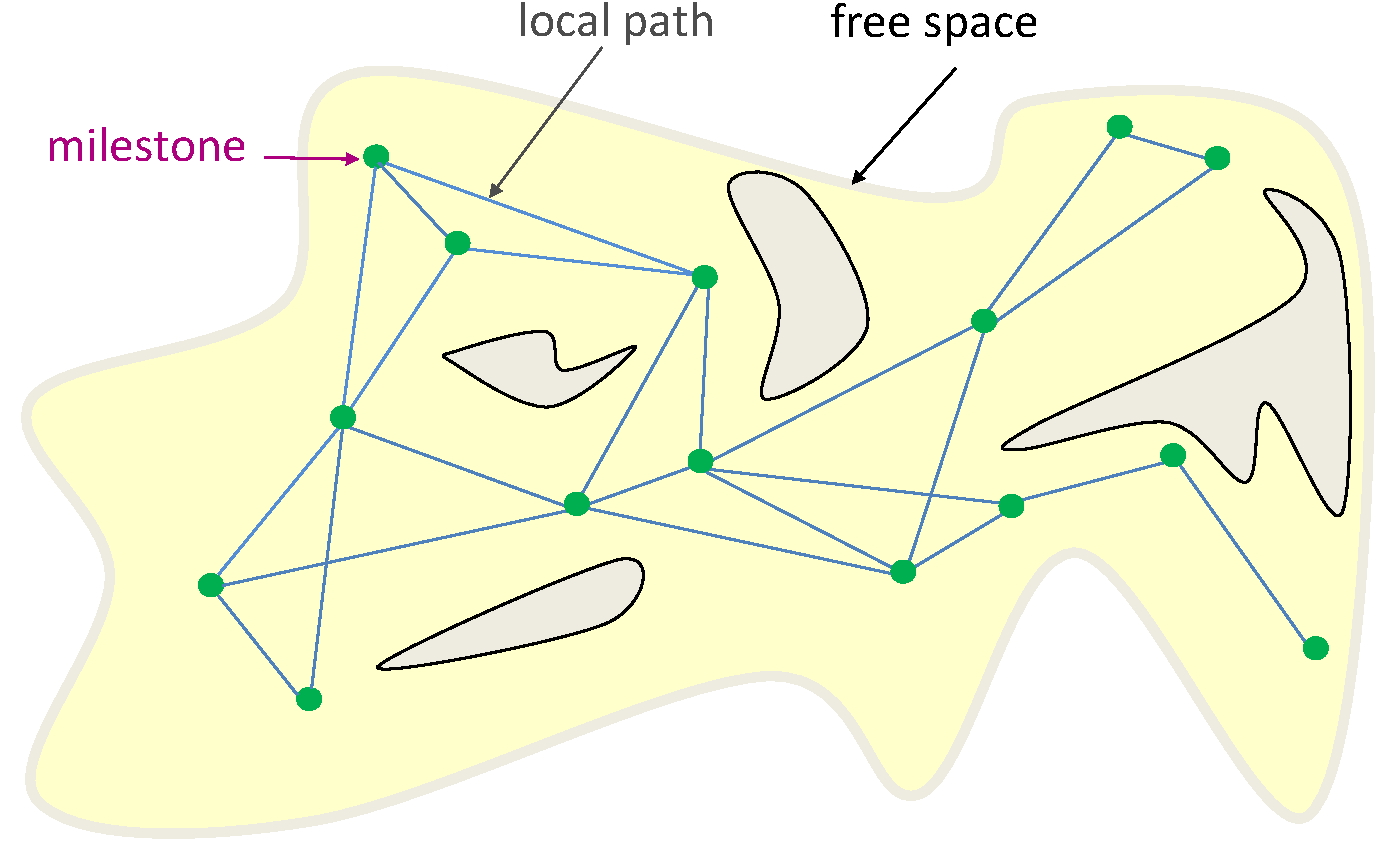
\includegraphics[width=0.49\linewidth]{figs/1/topology1.pdf}}
  \subfloat[Tree representation]{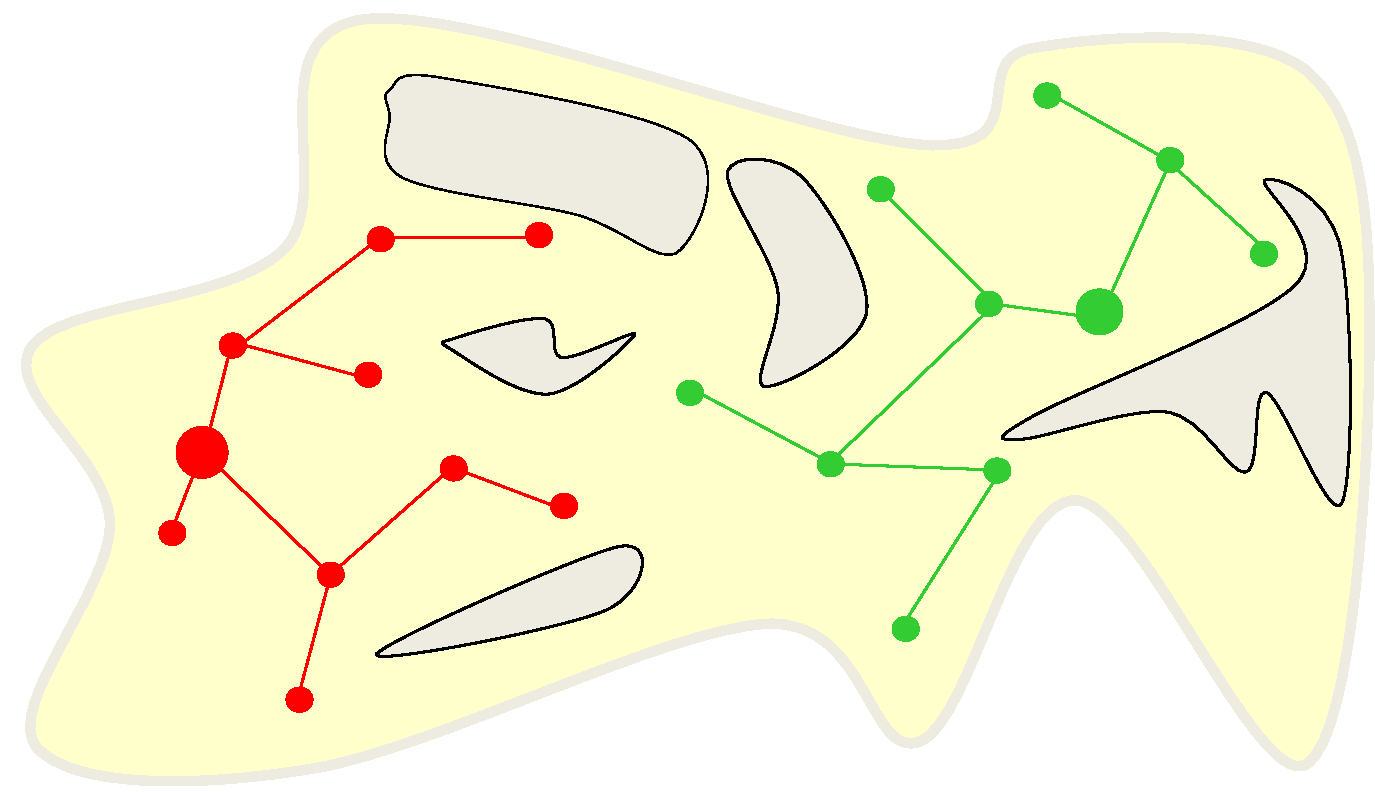
\includegraphics[width=0.49\linewidth]{figs/1/topology2.pdf}}
  \caption[Topology-based methods for configuration space computation]{Topology-based methods for configuration space computation. (a) Capture $\Cfree$ using a graph structure. (b) Capture $\Cfree$ using a forest of tree structures. The two figures are modified from Jean-Claude Latombe's lecture slides (\url{http://robotics.stanford.edu/\~{}latombe/cs326/2009/class5/class5.ppt}).}\label{fig:1:topologycspace}
\end{figure}




\section{Optimization in Configuration Space}
\label{sec:1:optimization}
Once an exact or approximate representation for the configuration space is computed, we next need to perform optimization in this $\Cspace$ representation. For example, the goal of motion planning is to compute a trajectory in $\Cspace$, as shown in Figure~\ref{fig:1:planning}. The trajectory should satisfy the following constraints: 1) it should be completely inside $\Cfree$; and 2) it should be feasible, e.g., for humanoid robots, the robot should not fall down when following the trajectory. Moreover, 
it is preferable for the trajectory to be optimal under some metric. For instance, the optimal trajectory could be the shortest, take the least time to execute, or maintain the maximum distance from obstacles.
As a result, motion planning can be formalized as a constrained optimization problem in $\Cspace$. Similar formulation can be applied to different applications, such as penetration depth computation~\cite{Zhang:2007:GPD,Zhang:2007:AFP,Zhang:2008:ICRA,Je:2012:PRP}.


\begin{figure}[!htb]
  \centering
  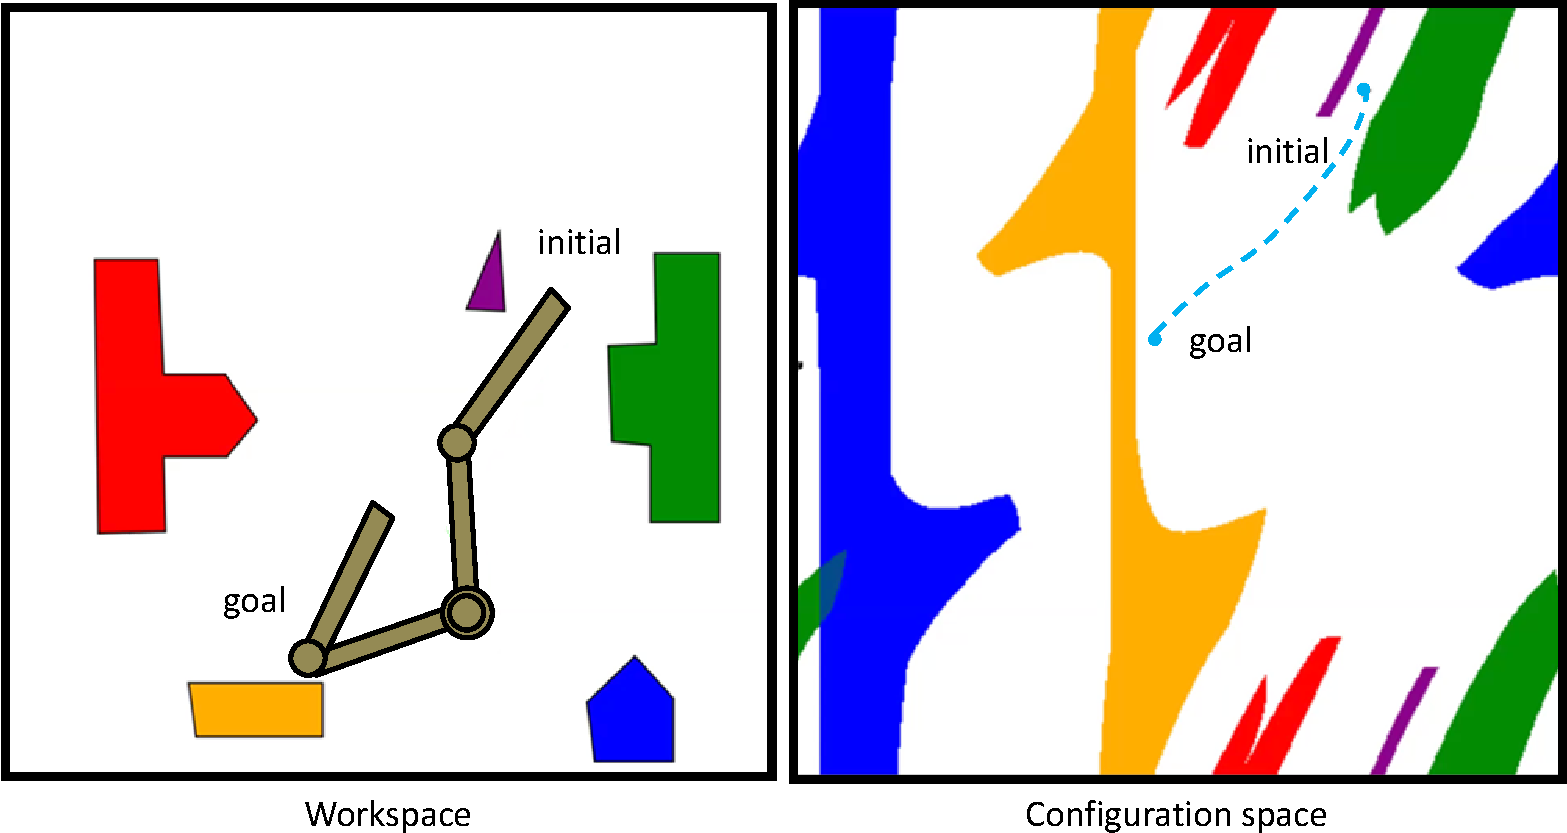
\includegraphics[width=\linewidth]{figs/1/planning-crop.pdf}
  \caption[Motion planning in workspaces and in configuration spaces]{Motion planning in workspaces and in configuration spaces. The left figure shows obstacles (with different colors) and a 2-linked robot in the workspace (both the initial and goal settings). The right figure shows the configuration space corresponding to the workspace in the left figure, where different colors describe the correspondence between obstacles in the workspace and obstacles in the configuration space. The blue curve is a trajectory connecting the initial and goal configurations, and is the result of motion planning algorithm. This figure is modified from~\cite{cspaceJapplet}. \label{fig:1:planning}}
\end{figure}


Optimization in $\Cspace$ is usually computationally expensive, especially for a high-dimensional $\Cspace$ with a complicated structure and topology. To illustrate the computational challenge for $\Cspace$ optimization problems, we take motion planning in $\Cspace$ as an example. Theoretically, motion planning using the exact representation of $\Cspace$ has high computational complexity. Planning algorithms are considered to be `complete' if for any planning problem instance, the algorithm will either find a solution or will correctly report that no solutions exists. Complete planning algorithms have been proved to be PSPACE-hard~\cite{Reif:1979:CMP} and PSPACE-complete~\cite{Canny:1988:AGC}, and kinodynamic motion planning (i.e., motion planning with simple kinematic or dynamic constraints) has been shown to be NEXPTIME-hard~\cite{Canny:1988:CKP}. 
The decidability is still unknown for motion planning with general differential constraints~\cite{Cheng:2007:DMP}. When the approximate representation of $\Cspace$ is used (e.g., using a graph or forest to approximate the connectivity of $\Cfree$), there exist approximate motion planning algorithms that provide guarantees of probabilistic completeness~\cite{Kavraki96,Kuffner00} and/or asymptotic optimality~\cite{Sertac:IJRR:2011}. The complexity of these approximate motion planning algorithms is usually bounded by $\mathcal O(n\ln n)$ where $n$ is the number of configuration samples used in the approximate representation of $\Cspace$~\cite{Sertac:IJRR:2011}. Since $n$ can be very large when $\Cfree$ has narrow passages and/or high dimensionality~\cite{Hsu:2006:ijrr}, the performance of these approximate algorithms is still far from real-time.

Various planning methods related to $\Cspace$ have been proposed in the past decades, including optimization-based planning algorithms such as CHOMP~\cite{Ratliff:2009} and TrajOPT~\cite{John:2013:FLO}, and search-based algorithms such as Anytime A*~\cite{Likhachev05anytimedynamic}. For motion planning of high-DOF (degrees-of-freedom) robots, most of the practical methods are based on randomized algorithms, including Probabilistic Roadmap (PRM)~\cite{Kavraki96} and Rapidly Exploring Random Tree (RRT)~\cite{Kuffner00}.


\section{Uncertainty Modeling in Configuration Space}
\label{sec:1:uncertainty}
Most prior techniques assume that an exact geometric representation is known for the robot and obstacles in the environment. This is reasonable in applications such as computer graphics, CAD, and simulation, where the geometric representation of synthetic objects is available. As a result, there is no ambiguity about the collision status of any configuration $\mathbf q \in \Cspace$: either $\q \in \Cfree$ and is collision-free or $\q \in \Cobs$ and is in-collision.

Unfortunately, this exact geometric representation assumption may not hold when we are dealing with real-world robots that interact with the physical environment. In the real world, sensors do not provide exact geometric representation, but rather noisy point clouds. The noise may arise from device noise, limited field-of-view, sensor refresh latency, synchronization error, or even occlusions. For noisy geometric representations, we cannot deterministically compute the collision status of a given configuration $\q$. Instead, $\q$ may lie in $\Cfree$ with probability $p$ and lie in $\Cobs$ with probability $1-p$, where $0 \leq p \leq 1$. Computing $p$ for any configuration $\q \in \Cspace$ is an open problem not studied in previous work.

The problem of modeling uncertainty in the configuration space has many applications. For example, it can be combined with motion planning algorithms to compute a trajectory that minimizes the probability to collide with the obstacles, which would improve the safety of robot navigation. Moreover, it can extend classical computational geometry algorithms to handle noisy sensor data, such as Minkowski sums~\cite{Varadhan:2006:TPA} and offsets~\cite{Choi:1997:CAD}.

\section{Thesis Statement}

Our thesis is as follows:

\textit{High-dimensional configuration spaces can be efficiently approximated using machine learning and geometric algorithms, and used for optimization queries related to motion planning and proximity computations on exact and noisy datasets.}

\section{Main Results}
In support of our dissertation, we present new techniques for configuration space construction, optimization in configuration spaces, and modeling uncertainty in configuration spaces. First, we demonstrate how to convert the configuration space construction problem into a machine learning problem, and then use active learning to compute an approximate configuration space efficiently and robustly. We also discuss how to use instance-based learning techniques to incrementally compute an approximate configuration space, which enables robots to learn from their past experiences about task execution. Second, we provide parallel GPU-based algorithms to accelerate the optimization computations in the configuration space, which can allow for real-time planning computation in many challenging environments. Finally, we propose two different methods to model the uncertainty in the configuration space caused by noisy geometries. These two methods are then combined with active sensing techniques to enable robots to work reliably in environments with uncertainty.

\subsection{Efficient $\Cspace$ Construction}
In this part, we describe two different methods to compute an approximate representation of the configuration space. The first is a geometry-based method and the second is a topology-based method.

First, we present a novel technique to efficiently approximate $\Ccont$ between two rigid objects using machine learning techniques. We first generate a set of samples in $\Cspace$ using collision detection techniques. We use non-linear SVM-based regression to construct an initial (coarse) approximation of $\Ccont$. Then we use active learning techniques to refine this approximation so that it is close enough to the actual $\Ccont$. We provide error bounds on the learned approximate $\Ccont$ and evaluate performance on many complex benchmarks. Additionally, based on the computed configuration space, we present an algorithm to efficiently approximate the penetration depth between two rigid objects, which is important in physically-based simulation.

Second, we present a novel approach to incrementally construct an approximate representation of $\Cspace$ from the samples generated during prior executions of the planning algorithm. Our formulation stores the results of prior collision queries and local planning queries. This information is used to accelerate the performance of planners. We present fast and novel algorithms to perform $\knn$ ($k$-nearest neighbor) queries in high dimensional $\Cspace$ and derive tight bounds on their accuracy. Our approach is general, makes no assumptions about the sampling scheme, and can be used with various sample-based motion planners with only small changes to these planners. Additionally, we discuss how to use this method to enable the planner to learn from its past query instances.

\subsection{Efficient Optimization in $\Cspace$}
In this part, we present techniques to accelerate optimization computation in $\Cspace$ using capabilities of many-core GPUs. This includes a GPU-based parallel planning algorithm called g-Planner. In g-Planner, GPU improves performance by addressing two main bottlenecks of sample-based planning algorithms: collision detection and $k$-nearest neighbor search, which can take more than 95\% of the overall planning time. We present a new GPU-based parallel collision detection
algorithm, which is able to efficiently handle a large number (i.e., more than 100,000) of collision queries between objects of varying complexity and runs more than 60 times faster than single-core CPU
algorithms. For $\knn$ search queries, we describe a new approximate algorithm for $\knn$ search based on Locality-Sensitive
Hashing (LSH), which is a GPU-friendly algorithm with sub-linear complexity and bounded error. The resulting
parallel GPU-based $\knn$ is at least 50 times faster than the optimized single-core CPU implementation.

\subsection{Uncertainty Modeling in $\Cspace$}
In order to model configuration spaces for noisy geometric representations, we first discuss a probabilistic collision detection algorithm between two objects represented as noisy point clouds. We convert the collision detection problem into a two-class classification problem and use extended SVM algorithms to solve it. To improve the efficiency, we use a divide-and-conquer method to eliminate unnecessary computations. As opposed to only computing the binary result (i.e., collision or not) by prior collision detection algorithms, our approach computes a collision probability. Collision probabilities are useful for robotics applications that require detailed measure of collision status, such as grasping.

The point cloud representation has some problems when it is used for modeling a noisy environment. First, point clouds provided by many
sensors may be too dense for real-time processing. Second, point clouds can only model occupied
regions in the environment and cannot distinguish between unknown regions and open regions, which may impair motion planning. To address these issues, we further present efficient collision detection and
distance computation algorithms for environment data represented as an octree, which can model occupied,
unknown, and open regions. Our algorithm can provide a collision probability. Moreover,
our formulation also takes into account the fact that the sensor data usually arrives at a higher rate (i.e., point cloud streams), and it is
difficult to track objects precisely between different frames of sensor data. This algorithm is used to guide Willow Garage's PR2 robot to operate safely in
poorly mapped regions with dynamic obstacles.

\section{Organization}
The remainder of this dissertation is organized as follows.

 \begin{description}
 \item[Chapter~\ref{chp:APD}] presents a geometry-based configuration space approximation using active learning.
 \item[Chapter~\ref{chp:IBL}] describes a topology-based configuration space representation using instance-based learning.
 \item[Chapter~\ref{chp:GPlanner}] presents a GPU-based motion planning framework for probabilistic roadmaps.
 \item[Chapter~\ref{chp:GCollide}] describes the GPU-based collision detection used in GPU-based motion planning.
 \item[Chapter~\ref{chp:GLSH}] presents the GPU-based $k$-nearest neighbor used in GPU-based motion planning.
 \item[Chapter~\ref{chp:PCollide}] presents how to model the uncertainty for a configuration when the geometry is point cloud sensor data.
 \item[Chapter~\ref{chp:PCollide2}] improves the performance of the algorithm described in Chapter~\ref{chp:PCollide} on point cloud stream data.
 \item[Chapter~\ref{chp:Conclusion}] presents conclusions and future work.
 \end{description}



%\include{mainmatter/replanning}
%\include{mainmatter/simulation}
%\include{mainmatter/lqgdef}
%\chapter{Conclusions and Future Work}
\label{chp:Conclusion}
In this dissertation, we have addressed a variety of computational challenges related to configuration spaces, including configuration space construction, efficient optimization in configuration space, and modeling uncertainty in configuration space. As research in configuration space continues, we expect progress in all these areas and more. While there is always more to do, the work presented in this dissertation has addressed many of the important issues in this field.

To summarize the main results presented in this dissertation:
\begin{description}
\item[Configuration Space Construction using Active Learning] We presented a novel approach to the approximation of configuration spaces. The main idea is to sample the configuration space and approximate the contact space based on machine learning classifiers, in particular support vector machines.
Furthermore, we use active learning techniques to select the samples during precomputation. Additionally, we use the precomputed configuration space for efficiently approximating the global penetration depth between two rigid objects.
\item[Configuration Space Construction using Instance-based Learning] We used instance-based learning to improve the performance of sample-based motion planners. The basic idea is to store the prior collision results as an approximate representation of $\Cfree$ and $\Cobs$, and to replace the expensive exact collision detection query by a relatively cheap probabilistic collision query. We integrated approximate collision routines with various sample-based motion planners and observe $30-100\%$ speedup on rigid and articulated robots, by enabling the robots to learn from their past experience.
\item[Parallel Motion Planning Framework] We introduced a whole motion planning algorithm on GPUs. Our algorithm can exploit all the parallelism within the PRM algorithm, including the high-level parallelism provided by the PRM framework and the low-level parallelism within different components of the PRM algorithm, such as collision detection and graph search. This makes our work the first to perform real-time motion planning and global navigation in general environments using GPUs.
\item[Parallel Collision Detection] We introduced two novel parallel collision query algorithms for real-time motion planning on GPUs. The first algorithm is based on configuration-packet tracing, is easy to implement, and can improve parallel performance by performing more coherent traversals and reducing the memory consumed by traversal stacks. The second algorithm is based on workload balancing, and decomposes parallel collision queries into fine-grained tasks. The algorithm uses a light-weight task-balancing strategy to guarantee that all GPU cores are fully utilized and achieves close to peak performance on GPUs.
\item[Parallel $k$-Nearest Neighbor] We presented an efficient GPU-based parallel Bi-level LSH algorithm to perform approximate $k$-nearest neighbor search in high-dimensional space. The Bi-level scheme can provide $k$-nearest neighbor results with higher quality than previous methods. In addition, our parallel algorithm provides more than a 40-fold acceleration over using LSH algorithms on CPUs.
\item[Proximity Computation for Noisy Geometry] We presented a novel and robust method for contact computation between noisy point cloud data using machine learning methods. We reformulate collision detection as a two-class classification problem and compute the collision probability at each point using support vector machines. This algorithm can be accelerated by using bounding volume hierarchies and performing a stochastic traversal.
\item[Proximity Computation for Noisy Geometry Streams] We presented two approaches for efficiently performing collision and distance queries on sensor data. The first method amortizes the sensor data pre-processing overhead over all the queries, and is suitable for static or simple environments. The second method shortens the traditional pipeline by directly performing queries between the robot links and an octree that represents sensor data. This approach completely avoids the data pre-processing overhead, and is suitable for dynamic or complex environments. Additionally, we combine this method with active sensing to improve robot safeness in uncertain or dynamic environments.
\end{description}

\section{Limitations and Future Work}
Our work has some limitations that could be addressed by future work.
\begin{description}
\item[Configuration Space Construction using Active Learning]
The accuracy and running time of our learning-based configuration space construction algorithm is a function of the combinatorial complexity of the contact
space and the sampling scheme. It is possible that our method may not generate a sufficient number of samples in small,
isolated components of contact space, or may take a high number of iterations.
The overall approach is probabilistic, and all our error bounds are derived in terms of expected error.
For future work, the basic components of our method, such as SVM learning and collision detection, can be accelerated using GPU parallelism. We can use other active learning techniques to improve the sampling, as well as other classifiers or learning techniques to improve the accuracy or convergence of the approximate contact space. It would be useful to derive tight theoretical error bounds for active learning algorithms based on exploitation and exploration. It would also be useful to extend the approach to articulated models, and take into account self-collisions between various links.
In order to handle deformable models, we would like to develop incremental techniques that can refine the contact
space approximation for deformable objects.
\item[Configuration Space Construction using Instance-based Learning] First, we need to find methods to adjust LSH parameters adaptively so that the $\knn$ query becomes more efficient for varying dataset sizes. One possible approach is to change $L$ (the number of hash tables), because a small $L$ may provide sufficient $\knn$ candidates for a large dataset. Second, for samples in regions that are well-explored, we should avoid inserting their collision results into the dataset in order to limit the dataset size. Moreover, since prior collision results are stored in hash tables, we can efficiently update the data without high overhead. Thus, we can extend the instance-based learning framework to improve the performance of planning algorithms in dynamic environments. Lastly, we would like to evaluate performance in dynamic scenes.
\item[Parallel Motion Planning Framework] Our current parallel planning work is limited to the PRM planning algorithm, but it is possible to extend it for accelerating other widely-used planning algorithms, including RRT or optimization-based planners. In addition, we are interested in extending GPU planning algorithms to high-DOF articulated models. We are also interested in using exact algorithms for local planning. Moreover, we hope to apply our real-time algorithms to dynamic scenarios.
\item[Parallel Collision Detection] We are interested in using more advanced sampling schemes with the GPU-based planner, to further improve its performance and deal with narrow passages. Furthermore, we would like to
modify the planner to generate smooth paths that take into account kinematic and dynamic constraints.
\item[Parallel $k$-Nearest Neighbor] We hope to test our algorithm on more real-world datasets, including images, videos, and so forth. We also need to design efficient out-of-core algorithms to handle very large datasets (e.g., $>$ 100GB), as the on-chip memory on a GPU is limited to a few GBs. We need to further analyze the quality of our bi-Level scheme on large spatial databases.

\item[Proximity Computations on Noisy Sensor Data] We need to test the performance of our algorithm on different robotic systems and evaluate its performance
on tasks such as planning and grasping. It would be useful to extend this approach to continuous collision checking, which takes into account the motion of the robot
between discrete intervals along its path. Similar probabilistic methods can also be developed for other queries,
including separation and penetration depth computation. Finally, we are interested in improving the algorithm to handle dynamic environments, where points may change position or can be added or removed from the environment due to movement, occlusion, or incremental data.
The algorithm for dynamic environments should handle incremental data efficiently and may benefit from various incremental techniques including incremental SVM~\cite{Gert:nips:2001} and BVH refitting techniques~\cite{Lauterbach10}.
\item[Proximity Computation for Streaming Noisy Sensor Data] We are interested in further improving the collision
checking and distance query implementations. We are also interested in
applications of this work to motion planning and active sensing. For example, we would like
to design strategies for gaining more information about uncertain or
unknown parts of the environment.
\end{description}







\chapter{Introduction}
\label{chp:intro}
Intelligent robots are becoming increasingly important in both industry and everyday life. In industry, rising labor costs are motivating manufacturers to consider using more robots in factories. For example, the average minimum wage in China has increased by more than 20 percent in 2012, while the supply of manufacturing robots has also increased by 51 percent in China~\cite{IFR:report}. 
Europe and USA exhibit similar trends: Intelligent robots are being designed in order to make workers more productive and make manufacturers more competitive in terms of price and quality. One recent example among these intelligent robots is the new ``Baxter'' robot~\cite{Brooks:2012:Baxter}, which is equipped with software that enables the robot to learn various tasks from human demonstration, recognize different objects, and react intelligently to external forces. Intelligent robots are expected to assist people in everyday life. In the future, such robots are expected to perform various tasks, including 1) household and care support, such as cooking and laundry; 2) healthy life support, such as chatting with the elderly and taking care of people with disabilities; and 3) labor support in unsafe working conditions such as chemical plants~\cite{Yamazaki:2012}. Several successful prototypes for assistant robots exist. For example, the PR2 robot from Willow Garage has been shown to assist people with severe physical disabilities such as quadriplegia~\cite{PR2HumanityWeb}; humanoid robots such as the HRP-4 can perform human-like actions and can communicate with people using speech~\cite{HRP-Cyber}. In addition to their applications in industry and everyday life, modern intelligent robots can be helpful in other areas, including autonomous vehicles~\cite{Montemerlo:2008:JSE}, medical and surgical intervention ~\cite{Bonfe:2012}, emergency and disaster rescue~\cite{Fukushima:2011}, and military tasks~\cite{AlphaDog:2012}.



\begin{figure}[!htb]
  \centering
  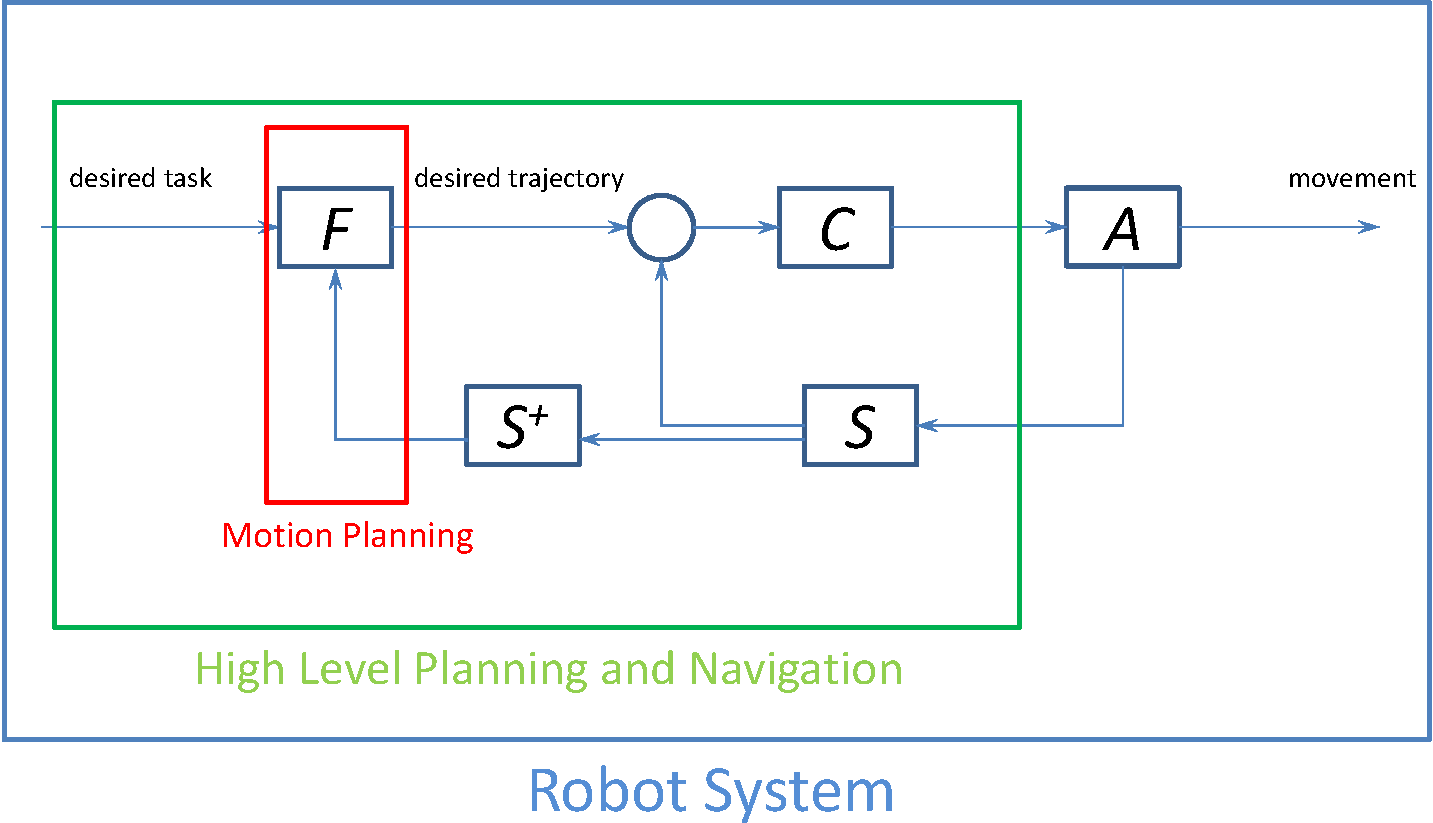
\includegraphics[width=\linewidth]{figs/1/pipeline-crop.pdf}
  \caption[Important hardware and software subsystems in a robot system]{Important hardware and software subsystems in a robot system. 1) Feed-forward system (F), including task planning, navigation strategy, motion planning and trajectory generation. 2) Control system (C), including kinematics, dynamics and control algorithms. 3) Actuator system (A), including motors, servos, transmissions, and so forth. 4) Sensor system (S), including various sensors such as camera, laser, IMU and related low level sensor data processing algorithms such as signal processing, estimation and fusion. 5) Sensor post-processing system (S$^+$), including localization, mapping, etc. The main software component of a robot system is the \emph{high level planning and navigation}, which determines the instructions sent to the actuator system, given the desired tasks to be executed. One important component of high level planning and navigation is \emph{motion planning}, which focuses on computing the trajectory from the environment description.}
  \label{fig:1:pipeline}
\end{figure}

The tremendous improvement in the design and availability of intelligent robots over the last decade is based on progress in many related areas, including computer vision, artificial intelligence, machine learning, control, sensor systems, and mechanical systems, which correspond to different components of an intelligent robot system (Figure~\ref{fig:1:pipeline}). For example, the SLAM (simultaneous localization and mapping) algorithm enables a robot to accurately track its position in an unknown environment~\cite{PR:2005}. In addition, with the help of advanced vision techniques, robots can now recognize and segment objects from background point clouds~\cite{Rusu:2009:IROS}. 
Compared to traditional industrial robots, one important feature of the modern intelligent robot system is \emph{high level planning and navigation}. Its main purpose is to compute low-level instructions based on high level descriptions for the tasks to be executed; these low-level instructions are then provided to the robot actuator system.
This planning and navigation component is composed of many different sub-components (Figure~\ref{fig:1:pipeline}) and there has been extensive work in this area, such as task planning~\cite{LPT:TPP:1989}, feedback from observation~\cite{KLP:2012:UPE,KLP:2011:NOW}, optimal control~\cite{Stengel:1994:OC}, and adaptive control~\cite{Astrom:1994:AC}.


One of the most important sub-systems of the high level planning and navigation component is the \emph{motion planning} system, which enables the robot to move safely from an initial position to a goal position without colliding with any static or moving obstacles in the environment. Motion planning enables robots to work efficiently and reliably in dynamic environments along with humans. Motion planning problems can be directly formalized and solved in the 3D workspace, for instance with the widely-used potential field algorithms~\cite{Khatib:IJRR:1986}. However, these workspace solutions cannot easily handle robots with different geometries and mechanical constraints. To overcome these difficulties, 
motion planning may be formalized and solved in a new space called the \emph{configuration space}~\cite{Lozano-Perez:1979:APC,LPT:APM:1981,LPT:SpatialPlanning:1983}. In the configuration space, a robot with a complex geometric shape in 3D workspace is mapped to a point robot and the robot's trajectory corresponds to a continuous curve in the high-dimensional configuration space (Figure~\ref{fig:1:planning}). Based on the configuration space formulation, the motion planning problem can be solved in two steps:

\begin{enumerate}
\item Construct a representation of the configuration space.
\item Perform optimization based on the computed representation.
\end{enumerate}

This motion planning pipeline based on configuration spaces is very successful and is adopted by many real-world planning applications that require optimal planning solutions. Many different representations for the configuration space have been proposed, including polyhedrons~\cite{Chazelle:ADS:1987}, semi-algebraic sets~\cite{Canny:1988:AGC,Canny:1988:CKP}, graphs~\cite{Kavraki96}, and trees/forests~\cite{Kuffner00}. Different optimization approaches have been proposed for different configuration space representations, including computing a shortest path, computing the minimum distance to the boundary of a closed set inside the configuration space, and so forth. Moreover, the same pipeline is also implicitly used in some motion planning algorithms for only computing a feasible path (i.e., a collision-free path that does not violate other constraints). For example, many variants of Rapidly Exploring Random Tree (RRT)~\cite{Kuffner00} use different heuristics to guide the search toward the goal configuration while growing a search tree structure as an approximate representation of the configuration space. Such a strategy can be viewed as a variant of the above pipeline, in which the configuration space construction alternates with the optimization computation.


However, this algorithmic pipeline based on $\Cspace$ still has many computational challenges:
\begin{enumerate}
\item Efficiently compute an approximate or exact representation for the configuration space is difficult, especially for high-DOF robots with high-dimensional configuration spaces. Such configuration space approximation problem would have exponential complexity (Section~\ref{sec:1:configconstruction}).
\item Many robotics applications require real-time planning in order to work reliably and efficiently in human environments with moving obstacles, but performing optimization in the computed representation for the configuration space can be time consuming (Section~\ref{sec:1:optimization}).
\item A robot in the real world depends on various sensors to acquire knowledge about its own state and the surrounding environments. Since the sensors provide noisy data, one important open problem involves enhancing the configuration space to consider robots and environments with noisy geometries. In contrast, previous work on configuration space based computations assume an exact representation of the robot and obstacles (Section~\ref{sec:1:uncertainty}).
\end{enumerate}


\section{Configuration Space}
\label{sec:1:configurationSpace}
The configuration space is a key concept used in classical mechanics to describe and analyze the motion of many important systems~\cite{Arnold:1989}. Generally, a \emph{configuration} $\q$ is a vector of independent parameters uniquely specifying the state of a system; a configuration space or $\Cspace$ is a collection of all possible configurations for a given system. For example, for a system of $n$ point particles, the configuration is a vector describing the positions of all the particles and the corresponding $\Cspace$ is $\mathbb R^{3n}$; the configuration of a 3D rigid body consists of its position and orientation, and the configuration space is $\SEcubic$ if both rotation and translation are allowed, and $\Rcubic$ if only translation is allowed; the configuration of an articulated object is the vector of all its joint angles.

The configuration space of a robot $A$ is composed of two components: \emph{collision-free space} $\Cfree = \{\q: A(\q) \cap B = \emptyset\}$ and \emph{in-collision space} or \emph{obstacle space} $\Cobs = \{\q: A(\q) \cap B \neq \emptyset\}$, where $B$ corresponds to the geometric representation of obstacles in the environment and $A(\q)$ corresponds to $A$ with the configuration $\q$. $\Cobs$ is a closed set and its boundary is denoted as the \emph{contact space} $\Ccont = \partial \Cobs$, which corresponds to the set of configurations where $A$ and $B$ just touch each other without penetration. Figure~\ref{fig:1:contactspace} shows an example of the $\Cspace$ of two objects where $\Ccont$ is highlighted with an orange curve.

\begin{figure}[!htb]
  \centering
  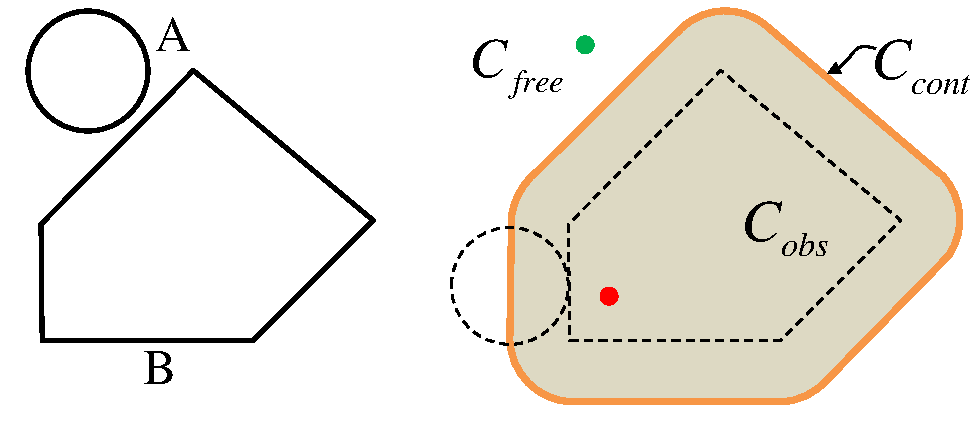
\includegraphics[width=0.6\linewidth]{figs/1/Ccont.pdf}
  \caption[The configuration space of two objects]{The configuration space of two objects. The orange curve highlights the contact space $\Ccont$ of $A$ and $B$. A point inside/on the orange curve belongs to
  $\Cobs$ and a point outside the orange curve belongs to $\Cfree$.
  The red and green points denote configurations in $\Cobs$ and $\Cfree$, respectively. Intuitively, $\Ccont$ is the boundary that separates in-collision and collision-free configurations.}
  \label{fig:1:contactspace}
\end{figure}

In the special case when $A$ and $B$ are both rigid objects and robot $A$ can only perform translation motion, $\Cobs$ is equal to the well-known Minkowski sum between $A$ and $B$: $\Cobs = A \oplus (-B) = \{\x = \x_A + \x_B | \x_A \in A, \x_B \in -B \}$. One example of the Minkowski sum is shown in Figure~\ref{fig:1:contactspace}. When robot $A$ can perform general motion (i.e., both translation and rotation), the geometry of $\Cobs$ is much more complicated, as shown by the 2D example in Figure~\ref{fig:1:cspaceSE2}.

\begin{figure}[!htb]
  \centering
  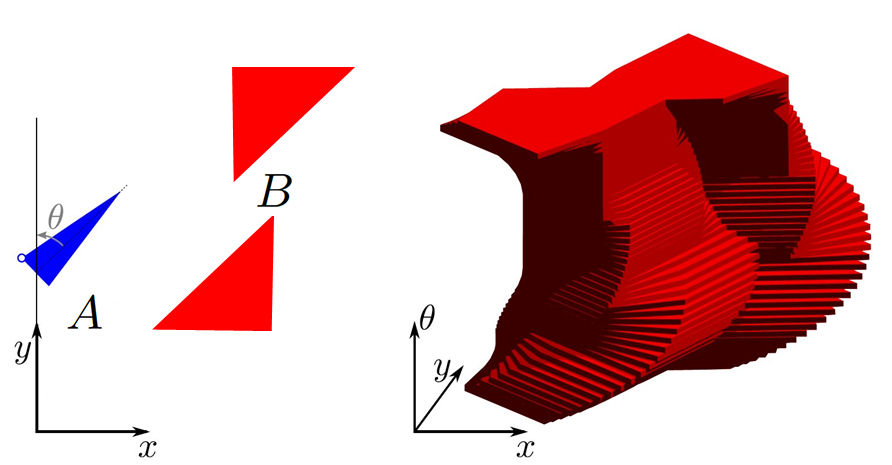
\includegraphics[width=0.9\linewidth]{figs/1/cspaceSE2.png}
  \caption[$\Cobs$ between 2D rigid objects $A$ and $B$]{$\Cobs$ between 2D rigid objects $A$ and $B$. For each rotation angle $\theta \in [0, 2\pi)$, we can compute the Minkowski sum between $A(\theta)$ and $-B$, where $A(\theta)$ is the resulting shape after rotating $A$ about the origin with $\theta$ degrees. When stacking the Minkowski sums for all angles $\theta$, we obtain the $\Cobs$ between $A$ and $B$. This figure is modified from an online image with unknown source.}
  \label{fig:1:cspaceSE2}
\end{figure}

Based on the notion of configuration space, the motion planning problem in 3D workspace can be reduced to path planning for a point robot in $\Cspace$, i.e., finding a curve in $\Cfree$ connecting the given initial and goal configurations of the robot.

\section{Configuration Space Construction}
\label{sec:1:configconstruction}
Before performing the motion planning computation in the configuration space, one prerequisite is to compute the geometry of $\Cspace$ in an appropriate representation (e.g., a graph or a surface). Since $\Cspace = \Cfree \cup \Cobs$ and $\Cfree \cap \Cobs = \emptyset$, we only need to construct the representation for either $\Cfree$ or $\Cobs$. Another equivalent solution is to compute $\Ccont$, the boundary between $\Cfree$ and $\Cobs$.

Previous work on configuration space construction can be categorized into two different methods: geometry-based and topology-based. Geometry-based methods compute the exact geometric representation of the configuration space while topology-based methods capture the connectivity of the configuration space.

Geometry-based methods are usually limited to low-dimensional configuration spaces, due to the combinatorial complexity involved in computing the boundary of $\Cobs$ for high-dimensional configuration spaces. Most previous work has focused on the special case when objects $A$ and $B$ are rigid bodies only performing translational motion. As mentioned in Section~\ref{sec:1:configurationSpace}, the resulting $\Cobs$ is the Minkowski sum between $A$ and $-B$. Even for this special case, the computational complexity involved in computing $\Cobs$ is still high: the complexity is $\mathcal O(mn)$ when $A$ and $B$ are both convex-objects and is $\mathcal O(m^3n^3)$ when $A$ and $B$ are both non-convex objects~\cite{Halperin:2002:RGC}, where $m$ and $n$ are the number of triangles in $A$ and $B$, respectively. In addition to the high complexity, most existing implementations for computing the Minkowski sum are prone to challenges that arise in the context of 3D geometric algorithms. In particular, these implementations are 1) not robust to numerical errors, and 2) susceptible to degeneracies (i.e., cannot reliably handle polygon soups or meshes with holes). Recent work has proposed methods~\cite{Lien:2008:CMS,Lien:2007:ACD,Lien:2009:ASM} for computing the approximate Minkowski sum efficiently and reliably, but these methods are also prone to robustness issues and can have high complexity in terms of dealing with complex objects. Options other than the Minkowski sum exist for computing  $\Cobs$. For example, Varadhan et al. compute the $\Cobs$ for 2D objects with rotation and translation by approximating the $\Cobs$ with an adaptive grid~\cite{Varadhan:2006:TPA}; Zhang et al. compute an approximation to 4D $\Cspace$ using cell decomposition~\cite{Zhang:2007:IROS}.

Topology-based methods capture the connectivity of the configuration space. Most previous approaches attempt to capture the connectivity of $\Cfree$ using sampling techniques~\cite{Kavraki96,Kuffner00}. The basic idea is first to generate random samples (called milestones) in $\Cfree$ and then organize these samples using a graph structure or a forest of tree structures (Figure~\ref{fig:1:topologycspace}). As the topology of $\Cfree$ can be rather complex, and
may consist of multiple components or small, narrow passages, it is hard to capture the full connectivity of $\Cfree$ using random sampling. There is extensive work on improving the connectivity computation by using different sampling strategies~\cite{Amato:1998:OOP,Boor:1999:ICRA,Hsu:1998:FNP,Rodriguez:2006,Zhang:2008:ICRA,Zheng:2005}. Recent work attempts to capture the topology of both $\Cfree$ and $\Cobs$~\cite{Jory:2011:IROS}. Topology-based methods can compute an approximate $\Cspace$ representation much faster than geometry-based methods. However, these methods do not work well with narrow passages and can be slow for high-DOF robots.


\begin{figure}[!htb]
  \centering
  \subfloat[Graph representation]{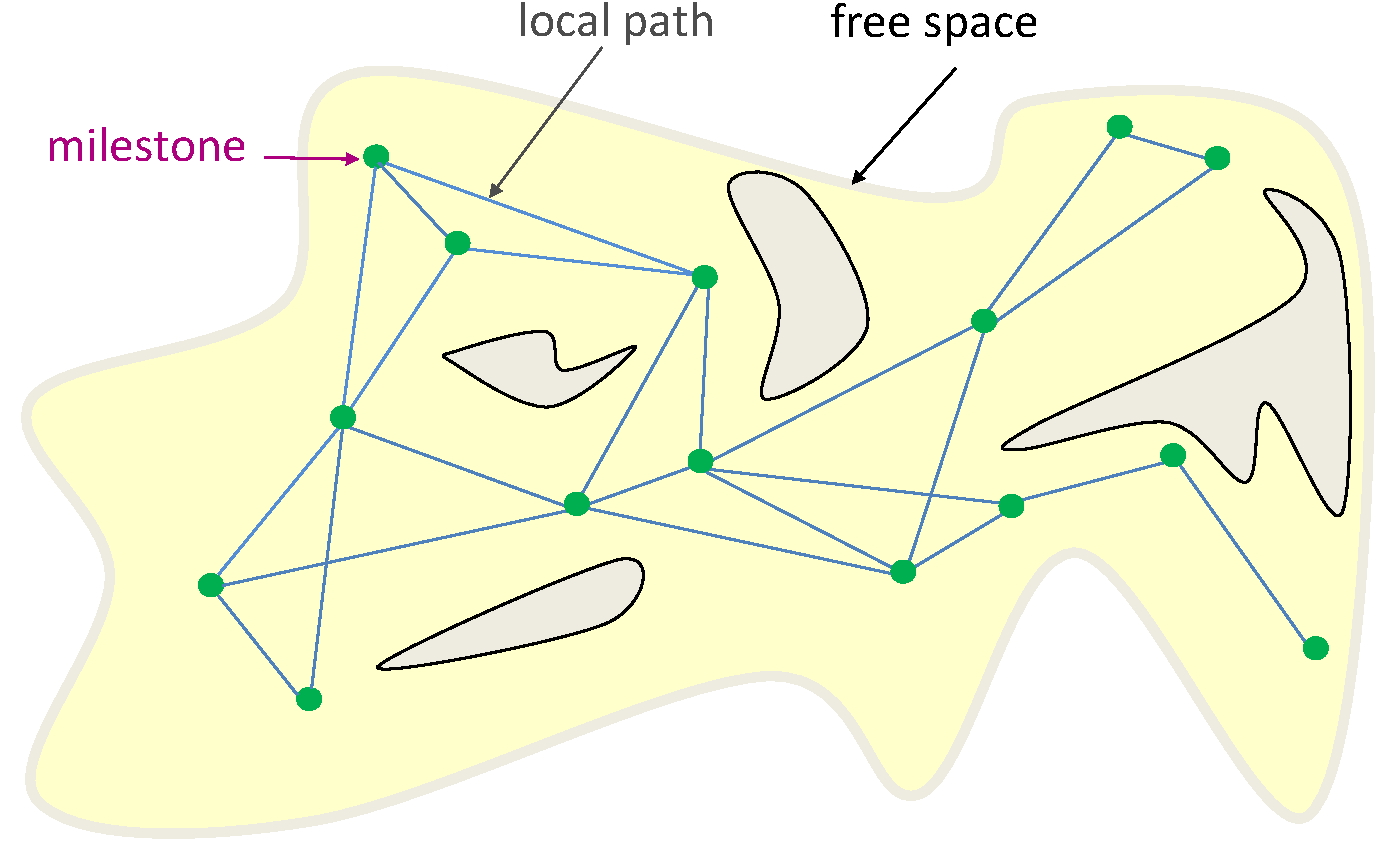
\includegraphics[width=0.49\linewidth]{figs/1/topology1.pdf}}
  \subfloat[Tree representation]{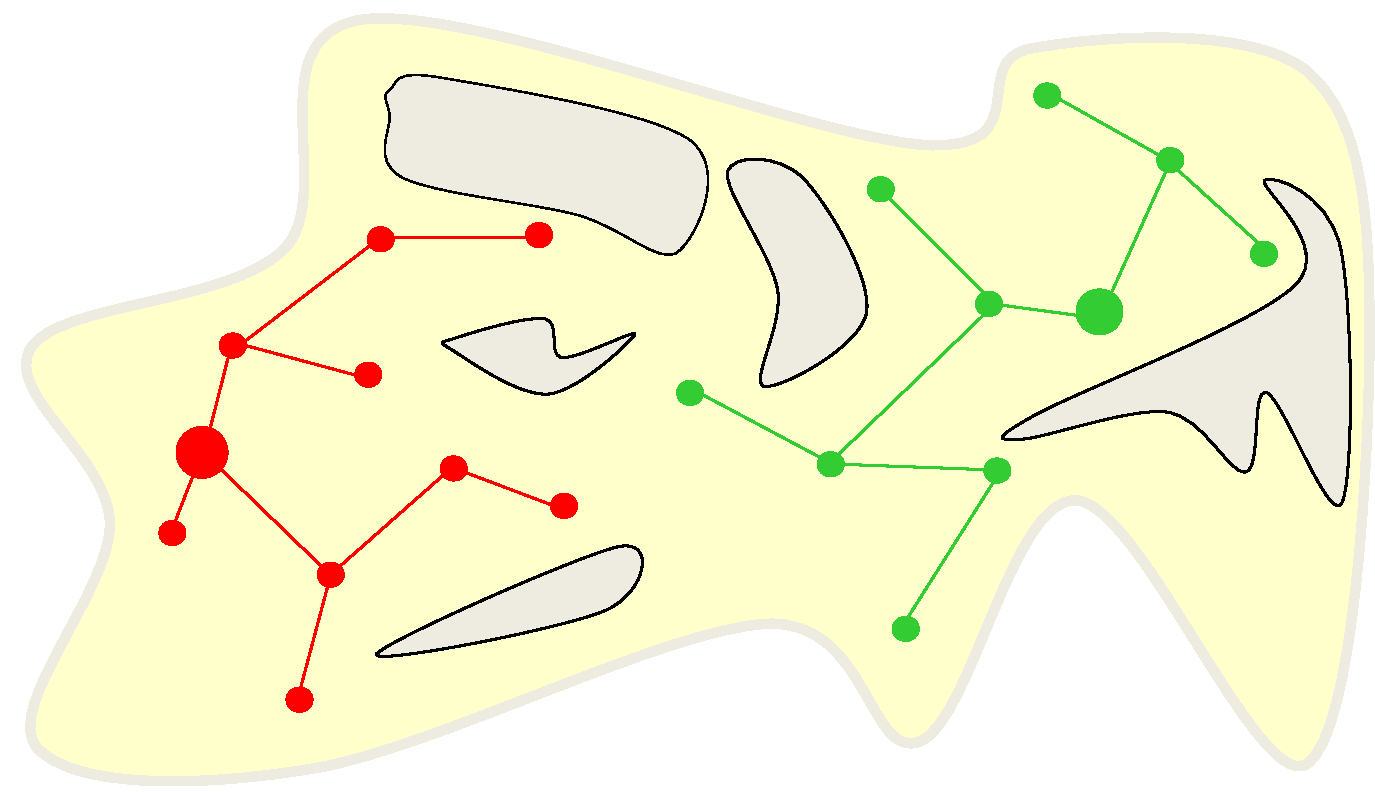
\includegraphics[width=0.49\linewidth]{figs/1/topology2.pdf}}
  \caption[Topology-based methods for configuration space computation]{Topology-based methods for configuration space computation. (a) Capture $\Cfree$ using a graph structure. (b) Capture $\Cfree$ using a forest of tree structures. The two figures are modified from Jean-Claude Latombe's lecture slides (\url{http://robotics.stanford.edu/\~{}latombe/cs326/2009/class5/class5.ppt}).}\label{fig:1:topologycspace}
\end{figure}




\section{Optimization in Configuration Space}
\label{sec:1:optimization}
Once an exact or approximate representation for the configuration space is computed, we next need to perform optimization in this $\Cspace$ representation. For example, the goal of motion planning is to compute a trajectory in $\Cspace$, as shown in Figure~\ref{fig:1:planning}. The trajectory should satisfy the following constraints: 1) it should be completely inside $\Cfree$; and 2) it should be feasible, e.g., for humanoid robots, the robot should not fall down when following the trajectory. Moreover, 
it is preferable for the trajectory to be optimal under some metric. For instance, the optimal trajectory could be the shortest, take the least time to execute, or maintain the maximum distance from obstacles.
As a result, motion planning can be formalized as a constrained optimization problem in $\Cspace$. Similar formulation can be applied to different applications, such as penetration depth computation~\cite{Zhang:2007:GPD,Zhang:2007:AFP,Zhang:2008:ICRA,Je:2012:PRP}.


\begin{figure}[!htb]
  \centering
  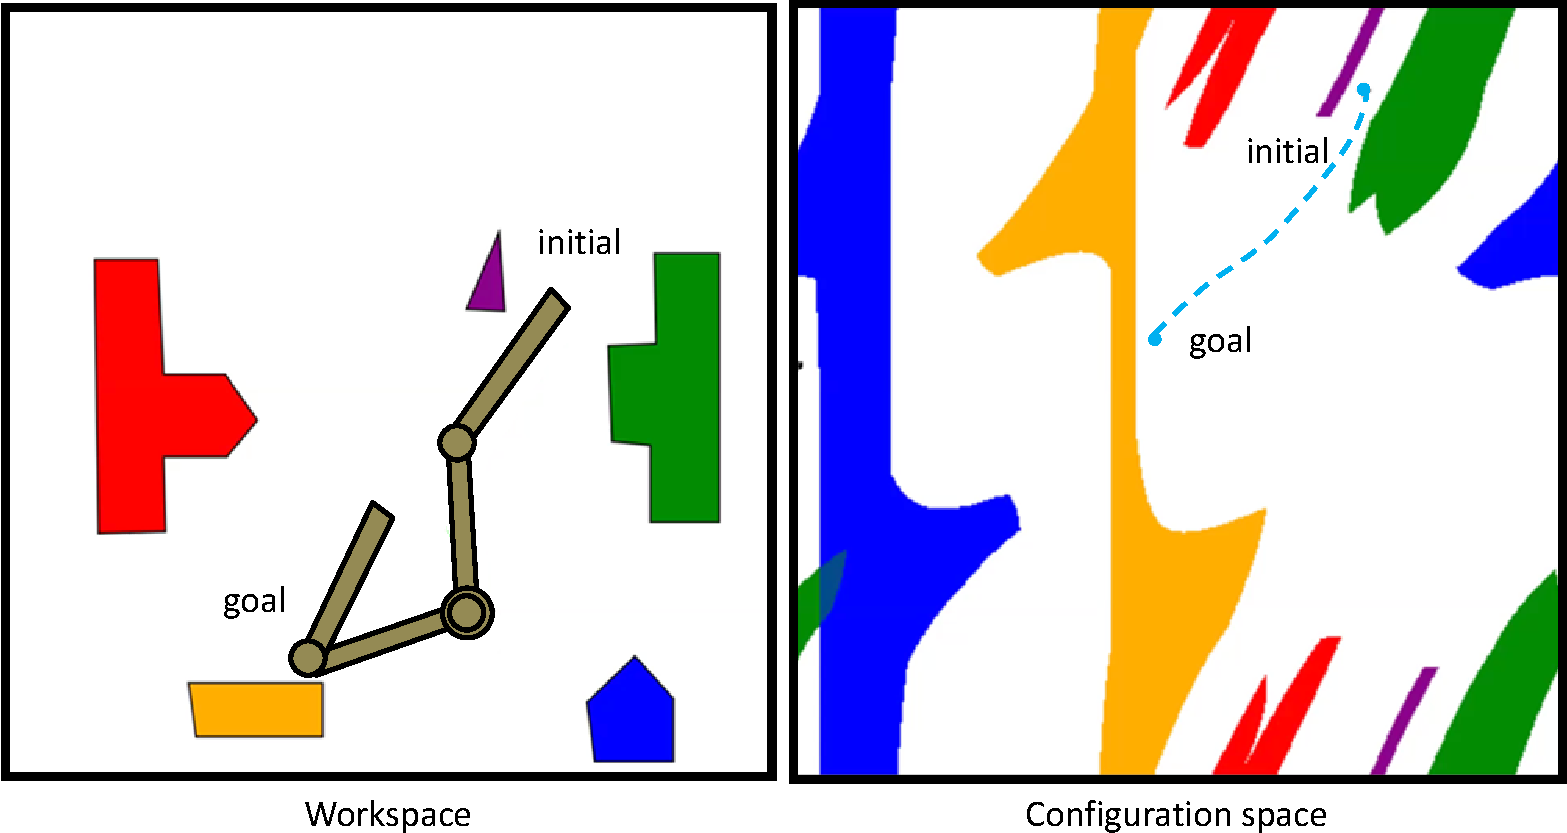
\includegraphics[width=\linewidth]{figs/1/planning-crop.pdf}
  \caption[Motion planning in workspaces and in configuration spaces]{Motion planning in workspaces and in configuration spaces. The left figure shows obstacles (with different colors) and a 2-linked robot in the workspace (both the initial and goal settings). The right figure shows the configuration space corresponding to the workspace in the left figure, where different colors describe the correspondence between obstacles in the workspace and obstacles in the configuration space. The blue curve is a trajectory connecting the initial and goal configurations, and is the result of motion planning algorithm. This figure is modified from~\cite{cspaceJapplet}. \label{fig:1:planning}}
\end{figure}


Optimization in $\Cspace$ is usually computationally expensive, especially for a high-dimensional $\Cspace$ with a complicated structure and topology. To illustrate the computational challenge for $\Cspace$ optimization problems, we take motion planning in $\Cspace$ as an example. Theoretically, motion planning using the exact representation of $\Cspace$ has high computational complexity. Planning algorithms are considered to be `complete' if for any planning problem instance, the algorithm will either find a solution or will correctly report that no solutions exists. Complete planning algorithms have been proved to be PSPACE-hard~\cite{Reif:1979:CMP} and PSPACE-complete~\cite{Canny:1988:AGC}, and kinodynamic motion planning (i.e., motion planning with simple kinematic or dynamic constraints) has been shown to be NEXPTIME-hard~\cite{Canny:1988:CKP}. 
The decidability is still unknown for motion planning with general differential constraints~\cite{Cheng:2007:DMP}. When the approximate representation of $\Cspace$ is used (e.g., using a graph or forest to approximate the connectivity of $\Cfree$), there exist approximate motion planning algorithms that provide guarantees of probabilistic completeness~\cite{Kavraki96,Kuffner00} and/or asymptotic optimality~\cite{Sertac:IJRR:2011}. The complexity of these approximate motion planning algorithms is usually bounded by $\mathcal O(n\ln n)$ where $n$ is the number of configuration samples used in the approximate representation of $\Cspace$~\cite{Sertac:IJRR:2011}. Since $n$ can be very large when $\Cfree$ has narrow passages and/or high dimensionality~\cite{Hsu:2006:ijrr}, the performance of these approximate algorithms is still far from real-time.

Various planning methods related to $\Cspace$ have been proposed in the past decades, including optimization-based planning algorithms such as CHOMP~\cite{Ratliff:2009} and TrajOPT~\cite{John:2013:FLO}, and search-based algorithms such as Anytime A*~\cite{Likhachev05anytimedynamic}. For motion planning of high-DOF (degrees-of-freedom) robots, most of the practical methods are based on randomized algorithms, including Probabilistic Roadmap (PRM)~\cite{Kavraki96} and Rapidly Exploring Random Tree (RRT)~\cite{Kuffner00}.


\section{Uncertainty Modeling in Configuration Space}
\label{sec:1:uncertainty}
Most prior techniques assume that an exact geometric representation is known for the robot and obstacles in the environment. This is reasonable in applications such as computer graphics, CAD, and simulation, where the geometric representation of synthetic objects is available. As a result, there is no ambiguity about the collision status of any configuration $\mathbf q \in \Cspace$: either $\q \in \Cfree$ and is collision-free or $\q \in \Cobs$ and is in-collision.

Unfortunately, this exact geometric representation assumption may not hold when we are dealing with real-world robots that interact with the physical environment. In the real world, sensors do not provide exact geometric representation, but rather noisy point clouds. The noise may arise from device noise, limited field-of-view, sensor refresh latency, synchronization error, or even occlusions. For noisy geometric representations, we cannot deterministically compute the collision status of a given configuration $\q$. Instead, $\q$ may lie in $\Cfree$ with probability $p$ and lie in $\Cobs$ with probability $1-p$, where $0 \leq p \leq 1$. Computing $p$ for any configuration $\q \in \Cspace$ is an open problem not studied in previous work.

The problem of modeling uncertainty in the configuration space has many applications. For example, it can be combined with motion planning algorithms to compute a trajectory that minimizes the probability to collide with the obstacles, which would improve the safety of robot navigation. Moreover, it can extend classical computational geometry algorithms to handle noisy sensor data, such as Minkowski sums~\cite{Varadhan:2006:TPA} and offsets~\cite{Choi:1997:CAD}.

\section{Thesis Statement}

Our thesis is as follows:

\textit{High-dimensional configuration spaces can be efficiently approximated using machine learning and geometric algorithms, and used for optimization queries related to motion planning and proximity computations on exact and noisy datasets.}

\section{Main Results}
In support of our dissertation, we present new techniques for configuration space construction, optimization in configuration spaces, and modeling uncertainty in configuration spaces. First, we demonstrate how to convert the configuration space construction problem into a machine learning problem, and then use active learning to compute an approximate configuration space efficiently and robustly. We also discuss how to use instance-based learning techniques to incrementally compute an approximate configuration space, which enables robots to learn from their past experiences about task execution. Second, we provide parallel GPU-based algorithms to accelerate the optimization computations in the configuration space, which can allow for real-time planning computation in many challenging environments. Finally, we propose two different methods to model the uncertainty in the configuration space caused by noisy geometries. These two methods are then combined with active sensing techniques to enable robots to work reliably in environments with uncertainty.

\subsection{Efficient $\Cspace$ Construction}
In this part, we describe two different methods to compute an approximate representation of the configuration space. The first is a geometry-based method and the second is a topology-based method.

First, we present a novel technique to efficiently approximate $\Ccont$ between two rigid objects using machine learning techniques. We first generate a set of samples in $\Cspace$ using collision detection techniques. We use non-linear SVM-based regression to construct an initial (coarse) approximation of $\Ccont$. Then we use active learning techniques to refine this approximation so that it is close enough to the actual $\Ccont$. We provide error bounds on the learned approximate $\Ccont$ and evaluate performance on many complex benchmarks. Additionally, based on the computed configuration space, we present an algorithm to efficiently approximate the penetration depth between two rigid objects, which is important in physically-based simulation.

Second, we present a novel approach to incrementally construct an approximate representation of $\Cspace$ from the samples generated during prior executions of the planning algorithm. Our formulation stores the results of prior collision queries and local planning queries. This information is used to accelerate the performance of planners. We present fast and novel algorithms to perform $\knn$ ($k$-nearest neighbor) queries in high dimensional $\Cspace$ and derive tight bounds on their accuracy. Our approach is general, makes no assumptions about the sampling scheme, and can be used with various sample-based motion planners with only small changes to these planners. Additionally, we discuss how to use this method to enable the planner to learn from its past query instances.

\subsection{Efficient Optimization in $\Cspace$}
In this part, we present techniques to accelerate optimization computation in $\Cspace$ using capabilities of many-core GPUs. This includes a GPU-based parallel planning algorithm called g-Planner. In g-Planner, GPU improves performance by addressing two main bottlenecks of sample-based planning algorithms: collision detection and $k$-nearest neighbor search, which can take more than 95\% of the overall planning time. We present a new GPU-based parallel collision detection
algorithm, which is able to efficiently handle a large number (i.e., more than 100,000) of collision queries between objects of varying complexity and runs more than 60 times faster than single-core CPU
algorithms. For $\knn$ search queries, we describe a new approximate algorithm for $\knn$ search based on Locality-Sensitive
Hashing (LSH), which is a GPU-friendly algorithm with sub-linear complexity and bounded error. The resulting
parallel GPU-based $\knn$ is at least 50 times faster than the optimized single-core CPU implementation.

\subsection{Uncertainty Modeling in $\Cspace$}
In order to model configuration spaces for noisy geometric representations, we first discuss a probabilistic collision detection algorithm between two objects represented as noisy point clouds. We convert the collision detection problem into a two-class classification problem and use extended SVM algorithms to solve it. To improve the efficiency, we use a divide-and-conquer method to eliminate unnecessary computations. As opposed to only computing the binary result (i.e., collision or not) by prior collision detection algorithms, our approach computes a collision probability. Collision probabilities are useful for robotics applications that require detailed measure of collision status, such as grasping.

The point cloud representation has some problems when it is used for modeling a noisy environment. First, point clouds provided by many
sensors may be too dense for real-time processing. Second, point clouds can only model occupied
regions in the environment and cannot distinguish between unknown regions and open regions, which may impair motion planning. To address these issues, we further present efficient collision detection and
distance computation algorithms for environment data represented as an octree, which can model occupied,
unknown, and open regions. Our algorithm can provide a collision probability. Moreover,
our formulation also takes into account the fact that the sensor data usually arrives at a higher rate (i.e., point cloud streams), and it is
difficult to track objects precisely between different frames of sensor data. This algorithm is used to guide Willow Garage's PR2 robot to operate safely in
poorly mapped regions with dynamic obstacles.

\section{Organization}
The remainder of this dissertation is organized as follows.

 \begin{description}
 \item[Chapter~\ref{chp:APD}] presents a geometry-based configuration space approximation using active learning.
 \item[Chapter~\ref{chp:IBL}] describes a topology-based configuration space representation using instance-based learning.
 \item[Chapter~\ref{chp:GPlanner}] presents a GPU-based motion planning framework for probabilistic roadmaps.
 \item[Chapter~\ref{chp:GCollide}] describes the GPU-based collision detection used in GPU-based motion planning.
 \item[Chapter~\ref{chp:GLSH}] presents the GPU-based $k$-nearest neighbor used in GPU-based motion planning.
 \item[Chapter~\ref{chp:PCollide}] presents how to model the uncertainty for a configuration when the geometry is point cloud sensor data.
 \item[Chapter~\ref{chp:PCollide2}] improves the performance of the algorithm described in Chapter~\ref{chp:PCollide} on point cloud stream data.
 \item[Chapter~\ref{chp:Conclusion}] presents conclusions and future work.
 \end{description}



\chapter{Configuration Space Approximation \mbox{using} Active Learning} 
\label{chp:APD}

\section{Introduction}
\label{sec:2:intro}
Computing a high-quality configuration space representation is important for many applications, such as robotics~\cite{LPT:SpatialPlanning:1983}, physically-based simulation~\cite{Je:2012:PRP}, Minkowski sums~\cite{Varadhan:2006:TPA}, and offset computation~\cite{Choi:1997:CAD}. 
However, to compute an exact representation for a configuration space is time-consuming, because the complexity of this problem grows exponentially in the dimension of the configuration space. As a result, it remains a major challenge to represent and compute configuration spaces, especially for high dimensional ones.

\subsection{Main Results}
In this chapter, we present a novel algorithm to efficiently approximate a high-dimensional configuration space using machine learning techniques. The main idea is to generate samples in the configuration space and then use these samples to approximate the contact space $\Ccont$ by a separating surface that can correctly separate all the in-collision and collision-free samples. This separating surface is computed using SVM classification. Our method greatly reduces the required number of samples by leveraging incremental and active learning techniques. 
When the number of samples increases, the approximate contact space computed by our method can quickly converge to the exact contact space; we also provide bounds on the expected error in the approximate contact space. We evaluate performance of our algorithm on high-dimensional benchmarks.

Additionally, based on the approximate $\Ccont$ computed offline, we design a new method to efficiently approximate the penetration depth (PD) between two rigid objects. The penetration depth is the minimum amount of motion required to separate two intersecting objects. Our algorithm performs a nearest-neighbor query between a given query configuration and the precomputed $\Ccont$ approximation. Compared to prior techniques, our approach is more general and more reliable. Moreover, the runtime query only has a small overhead (a few milliseconds) and thus can be used for interactive applications. In practice, we are able to compute approximate PD with relative error less than 2-3\% by using a few thousand samples during the offline $\Ccont$ computation. We also use our PD algorithm to compute collision response between non-convex models in Box2D and Bullet physics engines. We observe more than an order of magnitude improvement in runtime performance over that of prior global PD algorithms.

\subsection{Organization}
The rest of this chapter is organized as follows. We survey related work on configuration space computation in Section~\ref{sec:2:related}. We introduce the notation and give an overview of our algorithm in Section~\ref{sec:2:overview}. The approach for approximating the configuration space using learning techniques is described in Section~\ref{sec:2:learning}. The approximate configuration space is then used for approximate PD computation, as discussed in Section~\ref{sec:2:approxPD}. We analyze the accuracy and convergence of our approximate PD algorithm in Section~\ref{sec:2:analysis}. The implementation details and experimental results are provided in Section~\ref{sec:2:result}. We give a detailed discussion about the limitation of our method in Section~\ref{sec:2:limitations}.

\section{Related Work}
\label{sec:2:related}
\subsection{Configuration Space Construction}
There is extensive work on configuration space computation in robotics, geometric computing, and related areas.
Configuration space computation can be reduced to the problem of computing the arrangement of contact surfaces~\cite{Varadhan:2006:TPA}.
However, this approach is prone to problems involving accuracy and robustness. Moreover, the worst-case complexity of the entire arrangement can be as high as $\mathcal O(n^k)$, where $n$ is the number of contact surfaces in the arrangement and $k$ is the dimension of the configuration space~\cite{Goodman:Rourke:1997}. Some techniques for approximating the configuration space in lower dimensions are based on generating a discrete number of slices~\cite{Sacks:SCS:1997}. In this case, the configuration space is composed of many ruled surface patches, i.e., through each point on a surface patch, there exists a straight line that lies on the surface. These ruled surface patches are generated by different contact configurations between a vertex of an object and an edge from the other objects. When the object motion is limited to translation, the resulting configuration space is equivalent to the Minkowski sum between two objects~\cite{Leonidas:CCRS:1987,LPT:SpatialPlanning:1983}. Minkowski sum computation reduces the problem to computing either an arrangement or a union of a large set of convex primitives, which can be still very difficult in practice.

\subsection{PD computation}
PD computation has been studied extensively in computer graphics,
geometric modeling, haptics, and robotics. We give a brief
overview of exact and approximate computation algorithms.

Penetration depth is the minimum amount of motion transformation required to separate two intersecting objects. This transformation may correspond to only translation and the resulting PD is called the \emph{translational PD}; when this transformation corresponds to both translation and rotation, the resulting PD is called the \emph{generalized PD}.

For convex polytopes, exact translational PD can be computed using
the Minkowski sum~\cite{Gino:2001:GDC,Agarwal:2000:CPD,Kim:2002:DEEP}.
For non-convex objects, the PD can be computed using a combination of convex decomposition, pairwise Minkowski sums, and union computation~\cite{Kim:2002:FPD}. These algorithms are applicable to closed polyhedral shapes. The union computation has a high computational complexity. To address this issue, it is often approximated using rasterization hardware~\cite{Kim:2002:FPD}.

Most practical techniques for translational PD compute local PD
or some approximation of global PD. Local PD algorithms only take
into account local overlapping features (vertices, edges, and faces),
and compute a transformation to separate those
features~\cite{Guendelman:2003:NRB,Redon:2006:AFM,Lien:2009:ASM,Tang:2009:IHD,Tang:2012:CPF}. For example, local intersection volume and its derivative are used for volume-based repulsion in~\cite{Wang12}.
Distance fields are also used for local translational PD
computation~\cite{Heidelberger04} and can be computed in realtime using GPUs.
Point-based Minkowski
sum approximation~\cite{Lien:2008:CMS} can also compute global translational PDs.

Exact generalized PD can be computed by constructing the
exact contact space and then searching the contact space for the
closest point to a given query~\cite{Zhang:2007:GPD}. However,
due to high time and storage complexity, most
generalized PD algorithms use optimization-based
techniques~\cite{Nawratil:2009:GPD,Zhang:2007:AFP,Je:2012:PRP,Tang:IGP:2013} and compute a locally
optimal solution based on local approximation of the contact space.

Machine learning techniques have been used for collision detection~\cite{Doshi:2007:ISRR,Pan:2011:ISRR}. However, these techniques cannot be used for PD computation directly. One reason is that in practice, checking for collisions is much easier than computing the PD between overlapping objects.

\section{Background and Overview}
\label{sec:2:overview}
In this section, we introduce our notation and give an overview of our approach. We first present PD formulation in terms of configuration space and then describe our approach to computing approximate $\Ccont$ using learning techniques, which is then used for efficient computation of approximate PD.

\subsection{Contact Space and PD Formulation}
\subsubsection{Contact Space}
As we mentioned in Section~\ref{chp:intro}, the contact space $\Ccont$ is the boundary of $\Cobs$ and is denoted as $\Ccont =\partial \Cobs$. We use the notation $c(\q) \in \{-1,+1\}$ to denote the collision state of a configuration $\q$, i.e., $c(\q)=+1$ if $\q \in \Cobs$ and $c(\q)=-1$ if $\q \in \Cfree$.

\subsubsection{PD Formulation}
\label{sec:2:overview:pdformulation}
We define global penetration depth as the minimum motion or transformation required to separate two intersecting objects $A$ and $B$~\cite{Agarwal:2000:CPD,Kim:2002:DEEP}:

\begin{align}
\label{eq:2:PDgdef} \text{PD}(A(\qa), B) = \min_{\q \in
\Ccont} \dist(\qa, \q),
\end{align}
where $\qa$ is an in-collision configuration and $\q$ is a
configuration that lies in the contact space $\Ccont$.
We use the notation $\dist(\cdot, \cdot)$ to represent the distance between two configurations,
which may correspond to any metric defined on the $\Cspace$. The
contact point or configuration for which PD$(A, B)$ attains its
minimal value is denoted as $\qc = \argmin_{\q
\in \Ccont} \dist(\qa, \q)$.

In this chapter, we focus on the translational and rotational motion. Different types of motion require different $\dist(\cdot,\cdot)$ metrics.
For translational PD ($\PDt$), the commonly used $\dist(\cdot, \cdot)$ is the standard Euclidean distance metric between vectors corresponding to the configurations. Many distance metrics have been proposed for generalized PD ($\PDg$) computation, including weighted Euclidean
distance~\cite{Wang:CBO:2012}, object norm~\cite{Je:2012:PRP,Tang:IGP:2013}, and displacement distance metric~\cite{Zhang:2007:AFP}. We use the displacement distance metric in our algorithm, which is defined as:
\begin{align}
\label{eq:PDgmetric}
\dist(\mathbf q_i, \mathbf q_j) = \mu_1 q_1^2 + \mu_2 q_2^2 + \mu_3 q_3^2 + q_4^2 + q_5^2 + q_6^2,
\end{align}
where $(q_1, q_2, q_3)$ and $(q_4, q_5, q_6)$ measure the relative rotation and the relative translation between two configurations $\mathbf q_i$ and $\mathbf q_j$, respectively. $(q_0, q_1, q_2, q_3)$ corresponds to the relative quaternion between these two configurations, where $q_0=(1- q_1^2-q_2^2-q_3^2)^{1/2}$. $\mu_i$ is the weight on the rotational component and is computed as~\cite{Zhang:2007:AFP}:
\begin{align}
\label{eq:PDgmetricMu}
\mu_1 = \frac{4}{\vol}I_{xx}, \ \ \  \mu_2 = \frac{4}{\vol}I_{yy}, \ \ \  \mu_3 = \frac{4}{\vol}I_{zz},
\end{align}
where $\diag(I_{xx}, I_{yy}, I_{zz})$ represents the diagonal of the inertia matrix of the object $A$ and $\vol$ is the volume of the object $A$. 


\subsection{Approximate $\Ccont$ Computation}
To construct a representation of the configuration space, we use an offline learning algorithm as shown in the left box in Figure~\ref{fig:2:pipeline}. We first generate a small set of uniform samples in a subspace of $\Cspace$ for two given objects. Next, we justify whether these configurations lie in $\Cfree$ or in $\Cobs$ by performing exact collision checking between the two objects. Given the collision states ($-1$ or $+1$) of all configuration samples, a coarse approximation to the contact space, $\LCSa$ (Figure~\ref{fig:2:pipeline}(b)), is computed using classifiers, where $\LCS$ stands for \emph{Learned Contact Space}. Next, we select new samples in $\Cspace$ to further improve the accuracy of the initial representation $\LCSa$ using active learning. During active learning, we either select samples that are far away from prior samples (\emph{exploration}) (Figure~\ref{fig:2:pipeline}(c)) or samples that are near $\LCSa$ (\emph{exploitation}) (Figure~\ref{fig:2:pipeline}(d)).
After the new samples are generated, we compute an updated
approximation $\LCSb$ (Figure~\ref{fig:2:pipeline}(e)) based on incremental
machine learning techniques. We repeat this process, generating a sequence of approximate representations
$\LCSa$, $\LCSb$, ..., with increasing accuracy. This iterative process is repeated until the
collision states of all the new samples can be correctly
predicted by the current approximation. The final result $\LCS$
(Figure~\ref{fig:2:pipeline}(f)) corresponds to a smooth surface approximation of the contact space.

\subsection{Approximate PD Computation}
Given the approximate representation of the contact space, we can
then compute the approximate global PD by performing a nearest-neighbor query in the $\Ccont$.
The definition of approximate penetration depth is analogous to the exact penetration depth in Equation~\ref{eq:2:PDgdef}:

\begin{align}
\label{eq:2:PDsdef} \overline{\text{PD}}(A(\qa), B) = \min_{\q \in \LCS}\dist(\qa, \q),
\end{align}

Thus, the accuracy of $\overline{\text{PD}}$ is determined by the accuracy of $\LCS$.

As shown in Figure~\ref{fig:2:pipeline}(g), given a relative configuration $\qa$, we perform
a nearest-neighbor search to find a configuration that is closest to the decision boundary $\LCS$ and then project it
onto $\LCS$. We denote this projection result as $\qc$.
Finally, the distance between $\qa$ and $\qc$ is computed using an appropriate distance metric $\dist(\cdot, \cdot)$ and the result is an approximation to the exact PD value.


\begin{figure}[!htb]
  \centering
  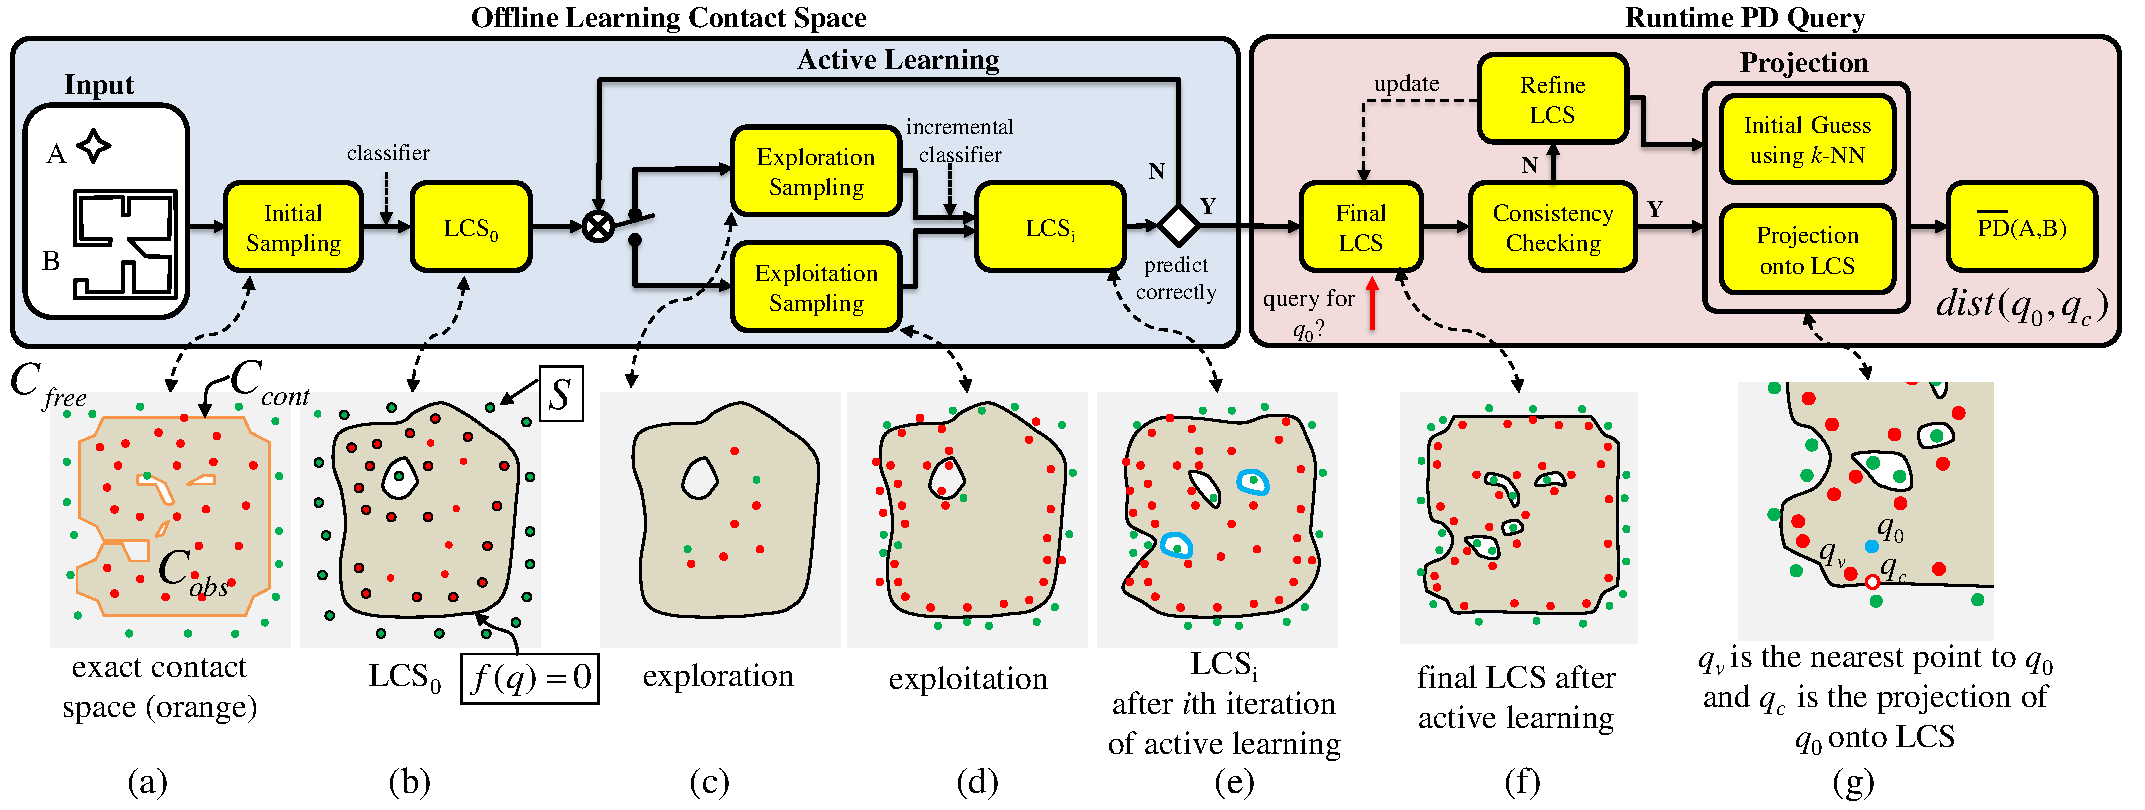
\includegraphics[width=\linewidth]{figs/2/pipeline.pdf}
  \caption[Offline computation pipeline for $\Ccont$ approximation and the runtime algorithm to compute the PD for a given query configuration]{This figure shows the offline computation pipeline for $\Ccont$ approximation and the runtime algorithm to compute the PD for a given query configuration. The different approximations of $\LCS$ are shown below the corresponding stages. We use green points to indicate collision-free configuration samples and red points to indicate in-collision samples.}
  \label{fig:2:pipeline}
\end{figure}

\section{Contact Space Construction via Machine Learning}
\label{sec:2:learning}
We now present our algorithm for the offline learning of the contact space and the computation of $\LCS$. Different stages of this algorithm
are shown in Figure~\ref{fig:2:pipeline}.

\subsection{Initial Sampling}
\label{sec:2:offline:uniform}

We perform uniform sampling in $\Cspace$ to obtain a set of configuration points. Rather than sampling the entire $\Cspace$,
we generate samples in a subspace that contains $\Ccont$. Given two objects $A$ and $B$, the contact space $\Ccont$ is contained in the in-collision space of their bounding volumes $BV(A)$ and $BV(B)$. We choose to use
axis-aligned bounding boxes (AABB) as the underlying BVs for $\PDt$
computation, due to their translational invariance in $\Rsqr$
and $\Rcubic$. Similarly, we use spheres as the underlying BVs for $\PDg$
computation due to their translational and rotational invariance in
$\SEsqr$ and $\SEcubic$.

The uniform sampling in the in-collision space of $BV(A)$ and $BV(B)$ can be implemented as follows. 
For $\PDt$ computation, the in-collision space of $BV(A)$ and $BV(B)$ is a box region, since it is the Minkowski sum of two axis-aligned bounding boxes. Samples uniformly distributed within this box region are guaranteed to cover the entire $\Ccont$.

For $\PDg$ computation, suppose that the given two bounding spheres are $(\mathbf c_A, r_A)$ and
$(\mathbf c_B, r_B)$, where $\mathbf c$ denotes a sphere center and $r$ denotes a sphere radius. We generate configuration samples for which these two bounding spheres are in collision. These samples correspond to all $(\mathbf R, \mathbf T)$ satisfying $\|\mathbf R \mathbf c_B + \mathbf T - \mathbf c_A\|_2 \leq r_A + r_B$, where $\mathbf R$ and $\mathbf T$ are the rotational and translational components of a configuration $\mathbf q$. We first generate one sample for the rotational component $\mathbf R$. For 2D rotation, we simply perform the uniform sampling within $[0, 2\pi]$; for 3D rotation, we use the method presented in~\cite{Shoemake:1992:URR} to sample $\SOcubic$ uniformly. After a random $\mathbf R$ is computed, the translational component $\mathbf T$ is uniformly distributed within a sphere $\|\mathbf T - (\mathbf c_A - \mathbf R \mathbf c_B)\| \leq r_A + r_B$; the uniform sampling within a sphere can be implemented using the well-known inverse-transform method. By repeating the above process many times, we can generate a sequence of $(\mathbf R, \mathbf T)$ uniformly distributed within the contact space of $A$ and $B$'s bounding spheres.

\subsection{Compute $\LCSa$} \label{sec:2:offline:model}
Given a set of $k$ samples from
$\Cobs(BV(A),BV(B))$, we perform exact collision queries between $A$ and $B$ to
check whether these samples are within in-collision space or not. Note that performing Boolean or discrete collision queries between complex models is a much easier problem compared to PD computation, as shown in Section~\ref{sec:2:analysis:timespacecomplexity}.
Our goal is to learn an approximate representation $\LCSa$ from these
configurations. In particular, $\LCSa$ corresponds to a decision function
$f(\q)=0$ that is fully determined by a set of configurations $\SV$
in $\Cspace$. We refer to $f(\q)$ as the \emph{classifier} and use it to
predict whether a given configuration $\q$ is collision-free
($f(\q)<0$) or in-collision ($f(\q)>0$). $\SV$ corresponds to the \emph{support vectors}, which are a
small subset of configuration samples used in learning.
Intuitively, $\SV$ are the samples that are closest to $\Ccont$.

Other options exist for computing the approximate contact space.
One alternative is to use surface fitting techniques to approximate the contact space by an implicit function, but this becomes more challenging for high-dimensional configuration spaces (e.g., 6-DOF $\Cspace$). Another possibility is to use regression-based learning techniques to approximate the contact space. However, such techniques typically require an improved or continuous approximation of PD values at these samples, which is much harder to compute compared to discrete collision queries.

\subsubsection{Nonlinear Classifier based on SVM}
\label{sec:2:offline:svm}
We use the SVM classifier~\cite{Vapnik:1995:NSL} to learn $\LCSa$ from
the initial sampling of $k$ configurations.
A SVM generates a decision function that is a smooth nonlinear surface. We use the
hard-margin SVM, as the underlying samples can
always be separated into collision-free and in-collision spaces. Intuitively, a SVM 
uses a function to map the given samples $\{\mathbf q_i\}$ from the \emph{input space} into a higher (possibly infinite) dimensional \emph{feature space}.
A SVM computes a linear
separating hyperplane characterized by parameters $\mathbf w$ and $b$. The hyperplane's maximal margin
is in the higher dimensional feature space. The hyperplane corresponds to a nonlinear separating surface in the input space. The $\mathbf w$ is the normal vector to the hyperplane, and the
parameter $b$ determines the offset of the hyperplane from the
origin along the normal vector. In the feature space, the distance between a hyperplane and the closest sample point is
called the `margin', and the optimal separating hyperplane should maximize this distance.
The maximal margin can be achieved by solving the following
optimization problem:
\begin{align}
\label{eq:2:svm1}
& \underset{\mathbf w, b}{\text{min}} & & \frac{1}{2}\|\mathbf w\|^2 & &  \\
& \text{subject to} & & c_i (\mathbf w \cdot \phi(\mathbf q_i) + b)
\geq 1, & & 1 \leq i \leq k. \notag
\end{align}
where $c_i \in \{-1,+1\}$ is the collision state of each sample ${\mathbf q_i}$.

Let $K(\mathbf q_i, \mathbf q_j) = \phi(\mathbf q_i)^T
\phi(\mathbf q_j)$ represent the kernel function (i.e., a function
used to calculate inner products in the feature space). The distance
between two points $\phi(\mathbf q_i)$ and $\phi(\mathbf q_j)$ in
the feature space can be computed as:
\begin{flalign}
\label{eq:2:svmdist}
&\|\phi(\mathbf q_i)-\phi(\mathbf q_j)\| \nonumber\\
&= \sqrt{K(\mathbf q_i, \mathbf q_i) + K(\mathbf q_j, \mathbf q_j)
- 2 K(\mathbf q_i, \mathbf q_j)}.
\end{flalign}
In our algorithm, we use the radial basis function (RBF) as the kernel:
$K(\mathbf q_i, \mathbf q_j) = \exp(-\gamma \|\mathbf q_i - \mathbf
q_j\|^2)$, where $\gamma$ is a positive parameter. In practice, we use $\gamma = 20$. We use the RBF kernel because it maintains the distance ranking
in both the input space and the feature space due to the fact that $\|\phi(\mathbf q_i) - \phi(\mathbf q_j)\|_2^2 = 2 - 2 \cdot \exp(-\gamma \|\mathbf q_i - \mathbf q_j\|_2^2)$.

The solution of Equation~\ref{eq:2:svm1} is a nonlinear surface in the
input space (and a hyperplane in the feature space) that separates
collision-free and in-collision configurations. This solution can be
formulated as:
\begin{align}
\label{eq:2:svmf} f(\mathbf q) = \mathbf w^* \cdot \phi(\mathbf q) +
b^* = \sum_{i=1}^k \alpha_i c_i K(\mathbf q_i, \mathbf q) + b^*,
\end{align}
where $\mathbf w^*$ and $b^*$ are the solutions of
Equation~\ref{eq:2:svm1} and $\alpha_i \geq 0$. 
The vectors $\mathbf q_i$ corresponding to the non-zero $\alpha_i$ are called
the \emph{support vectors}, which we denote as $\SV$. Intuitively, the support vectors
are those samples closest to the separating hyperplane
$f(\mathbf q) = 0$, as shown by the larger red and green points in
Figures~\ref{fig:2:pipeline}(b) and ~\ref{fig:2:pipeline}(g).
Thus, $\LCSa$ consists of an implicit function
$f_{\LCSa}(\q) = f(\q)$ and a set of samples
$S_{\LCSa}=S$ (i.e., the support vectors), which
are used to approximate the exact contact space.


\subsection{Refine $\LCSa$ using Active Learning}
\label{sec:2:offline:activelearning}
We refine $\LCSa$ using active learning. The
goal is to actively select new samples so that a better
approximate contact space representation, $\LCSb$, can be obtained by incorporating
these samples into $\LCSa$. We use a
combination of exploration and exploitation~\cite{Huang:2010:ALQ}.
The idea is to determine whether to explore
or to exploit by flipping a biased coin with a certain probability for landing on heads
(initially $0.5$). If the result is a head, we apply exploration;
if it is a tail, we apply exploitation. The probability of landing on heads is adjusted
according to the fraction of exploration samples' collision
states that are correctly predicted by the current $\LCSi$. The new
samples are used to update $\LCSa$ and generate a new approximation
$\LCSb$ (or refine from $\LCSi$ to $\LCSiplus$). We repeat the active
learning step until all the new samples can either be correctly
predicted by the current $\LCSi$, or the final result (represented
as $\LCS$) has sufficient accuracy to approximate $\Ccont$. Later in Section~\ref{sec:2:analysis}, we show that active learning results in improved convergence compared to uniform or random sampling schemes.


\subsubsection{Exploration}
$\LCSa$ may miss some holes or components corresponding to collision-free regions, if no initial samples were generated inside those regions. As a result, there may be some portions that $\LCSa$ may incorrectly classify, as shown in Figure~\ref{fig:2:pipeline}(c). In this case,
exploration refers to generating samples far away from prior
samples in order to explore the regions not well-sampled by the
current $\LCSi$. In our algorithm, we use random sampling to
explore these new regions (Figure~\ref{fig:2:pipeline}(c)). As
shown in Figure~\ref{fig:2:pipeline}(e), two new collision-free
regions (marked as blue curves) are found using exploration. After
each exploration sampling step, we compute the fraction of the new
samples that are not correctly predicted by $\LCSi$ to determine whether the exploration improves $\LCSiplus$.
If this cutoff fraction is large (e.g., $0.3$), then we increase the probability for exploration; otherwise we
decrease it.


\subsubsection{Exploitation}
Exploitation refers to generating samples near the decision
function of a given approximation $\LCSi$.

For exploitation, we use a simple method based on the \emph{maximal margin} property
of SVMs. The maximal margin
property~\cite{Vapnik:1995:NSL} states that in the feature space, the decision function
will have the same distance to support vectors with different
labels (i.e., collision-free or in-collision). In order to obtain a sample near the
decision function $f_{\LCSa} = 0$, we first choose a pair of support
vectors that are close to each other, but have opposite labels.
Based on the maximal margin property, the midpoint of the two
supporting vectors lies on or near the decision function.
\begin{figure}[!htb]
  \centering
  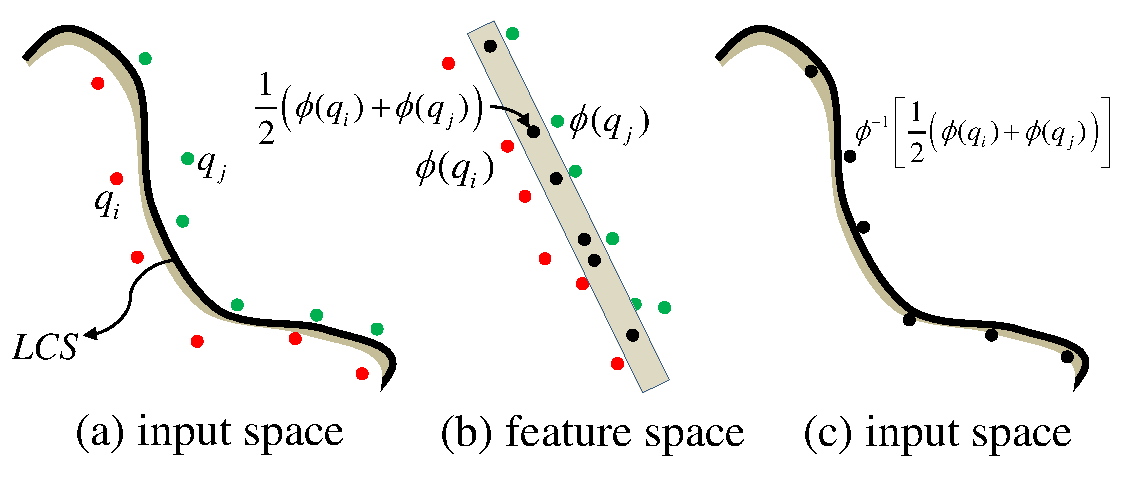
\includegraphics[width=0.6\linewidth]{figs/2/interpolation.pdf}
  \caption[Exploitation in SVMs]{Exploitation in SVMs:
  (a) support vectors are on different sides of the decision function ($\mathbf q_i$ and $\mathbf q_j$) in the input space;
  (b) their midpoints (black points) are computed in the feature space;
  (c) the pre-images of the midpoints lie near the decision function and can be used for exploitation.}
  \label{fig:2:interpolation}
\end{figure}
For nonlinear SVMs, the closest point and interpolation computations are
performed in the feature space. As shown in
Figure~\ref{fig:2:interpolation}, we first use the distance metric
mentioned in Equation~\ref{eq:2:svmdist} to find a pair of
supporting vectors $\mathbf q_i$ and $\mathbf q_j$. Next, we
compute their midpoint $\frac{1}{2}(\phi(\mathbf q_i) +
\phi(\mathbf q_j))$ (shown as black points in Figure~\ref{fig:2:interpolation}(b)). However, since the resulting midpoint may not have a pre-image in the input space, we search the input
space for a point $\q$ whose image $\phi(\q)$ in
feature space is closest to $\frac{1}{2}(\phi(\mathbf q_i) +
\phi(\mathbf q_j))$:
\begin{equation}
\begin{aligned}
\label{eq:2:preimage}
& \ \underset{\mathbf q}{\text{min}} & & \|\frac{1}{2}(\phi(\mathbf q_i) + \phi(\mathbf q_j)) - \phi(\mathbf q)\|_2 & \\
\Leftrightarrow & \ \underset{\mathbf q}{\text{max}} & & K(\mathbf q, \mathbf q_i) + K(\mathbf q, \mathbf q_j). &
\end{aligned}
\end{equation}
The solution is found using an optimization solver, in which the midpoint $\frac{\mathbf q_i +
\mathbf q_j}{2}$ in the input space is used as the initial guess. In our
benchmarks, this optimization solver tends to converge quickly
(in less than $10$ iterations).


\subsection{Incremental Learning}
\label{sec:2:incremental_learning}
Instead of computing a new decision function
from scratch using all the previous samples, we apply incremental
learning techniques to efficiently compute $\LCSiplus$ from
$\LCSi$. Incremental learning utilizes a small set
of new samples to update $\LCSi$. The decision function of $\LCSi$
serves as the initial guess for generating $\LCSiplus$. The incremental SVM~\cite{Karasuyama:2009:MID} can update
the current result generated using SVMs; the key is to retain the optimality condition of Equation~\ref{eq:2:svm1} (i.e., the Kuhn-Tucker condition) on all prior samples while adding new samples. This is achieved by adjusting the coefficients $\alpha_i$ and $b$ in Equation~\ref{eq:2:svmf} and by adjusting support vector set $\SV$. The coefficient adjustment and the support vector changes are guided by the gradient of the objective function in Equation~\ref{eq:2:svmf}.

\subsection{Terminating Active Learning}
Active learning terminates when either of these conditions has been satisfied:
\begin{enumerate}
    \item The collision states of all the new samples generated during
exploration and exploitation can be correctly predicted by the
current approximation $\LCSi$.
    \item The total number of samples used in active learning iterations is more than a user-specified threshold.
   \end{enumerate}
The first condition guarantees that all the configurations used for learning $\LCS$ are consistent (i.e., they can be correctly predicted by $\LCS$). This implies that the current $\LCS$ is a close approximation of the underlying contact space.
The second condition controls the error in PD computation. As more samples are used, we get a better approximation to $\Ccont$, and thereby a lower PD error.


\section{Approximate PD Computation}
\label{sec:2:approxPD}

We use the learned approximate contact space $\LCS$ to perform PD queries at
runtime. This section describes details on the runtime
algorithm. It consists of two parts: local $\LCS$ refinement based on consistency checks, and
computing the nearest configuration on $\LCS$.


\subsection{Local $\LCS$ Refinement}
Let $\qa$ be a configuration that corresponds to overlapping rigid objects $A$
and $B$. The exact collision check between these objects is performed using
bounding volume hierarchies. We also compute the approximate collision state corresponding to $\qa$ using $\LCS$: i.e., we
check whether ($f(\qa)>0$) as that corresponds to an in-collision configuration.
It is possible that the collision state predicted
using $\LCS$ may be different from that computed by the exact
algorithm, which implies that $\LCS$ is not sufficiently
accurate at approximating the contact space in the neighborhood of $\qa$.
In this case, we refer to $\qa$ as an \emph{inconsistent} configuration;
otherwise, it is consistent.
Generally, an inconsistent configuration occurs when the query is located in
a $\Cspace$ region that is not well sampled during the learning phase.

Our runtime algorithm first checks
whether a given query $\qa$ is consistent. If $\qa$ is inconsistent, $\qa$ corresponds to a collision-free configuration
predicted by $\LCS$ ($f(\qa)<0$) and its distance to $\LCS$ is
more than a user-specified error threshold. In this case, we locally refine
$\LCS$ by incorporating $\qa$ into $\LCS$ using incremental learning (Section~\ref{sec:2:incremental_learning}).
This local refinement of $\LCS$ improves the query efficiency and the accuracy of PD computation (Equation~\ref{eq:2:Errdef}).

During each runtime query, we perform an incremental learning step for an inconsistent
single configuration. This incremental learning has an runtime overhead of $\mathcal O(1)$.
Moreover, this local refinement step improves the accuracy of $\LCS$ in local
regions where more PD queries are potentially performed by an application during runtime. 
As a result, this step results in more accurate answers for those nearby queries by exploiting the spatial coherence in the configuration space.

\subsection{$\LCS$ Projection}
\label{sec:2:approxPD:projection}
Given a consistent configuration $\qa$, we search for the closest configuration
on $\LCS$ to compute the PD. In particular,
we \emph{project} $\qa$ onto the decision boundary $f_{LCS} = 0$ to obtain $\qc$, the nearest configuration on $\LCS$. In this case, the approximate
PD is computed using $\dist(\qa, \qc)$ function.
For SVM classifiers, the projection computation can be reduced to a constrained
optimization problem:
\begin{equation}
\begin{aligned}
\label{eq:projection}
 & \underset{\mathbf q}{\text{min}} & \dist(\mathbf \qa, \mathbf q), & & \text{subject to} & & f_{LCS}(\mathbf q) = 0.
\end{aligned}
\end{equation}
A key challenge is to perform this projection efficiently and ensure that the optimization algorithm is not
trapped in a local minima, as the shape of the decision function can be complicated.
In order to deal with these issues, we perform the computation in two phases:
first, we perform a $k$-nearest-neighbor search in $\Cspace$ to compute the configuration
$\qv \in S_{LCS}$ (i.e., the configuration among the support vectors) that is closest to $\qa$ based on our $\dist(\cdot, \cdot)$ metric. Next, we
use $\qv$ as an initial guess to the constrained optimization problem and compute the closest configuration on the $\LCS$.
Since $\qv$ is a configuration very close to the decision boundary, it serves as a good initial guess.

We use different nearest-neighbor (NN)  search algorithms to compute $\qv$, depending on whether we are
performing this search in 3-DOF $\Cspace$ or 6-DOF $\Cspace$. For 3-DOF $\Cspace$, $\dist(\cdot, \cdot)$ corresponds to the Euclidean distance metric, and we use a kd-tree to accelerate NN computation. For 6-DOF $\Cspace$, we use a hierarchical clustering algorithm for efficient NN search~\cite{Muja:2009:FAN}.

\section{Analysis}\label{sec:2:analysis}
In this section, we analyze various characteristics of our algorithm, including errors in PD computation, benefits of active learning, and time and space complexity.

\subsection{Error in $\LCS$ and in PD Computation}
\label{sec:errordefine}
Since our approach is probabilistic, we compute a bound on PD approximation based on \emph{expected
error}~\cite{Vapnik:1995:NSL}, which corresponds to the average error
when $\LCS$ is applied to predict the
collision state or PD value for a new configuration in the $\Cspace$.
This error can be expressed as:
\begin{equation}
\label{eq:2:Errdef0} e_{\text{col}} = \mathbb E
\left|e_\text{cs}(\mathbf q) \right|,
\end{equation}
where $e_{\text{cs}}(\q)=0$ if $\q$ is a consistent configuration, and $e_{\text{cs}}(\q)=1$ if $\q$ is inconsistent.
Expectation $\mathbb E$ is calculated from a series of
random configurations or queries. Typically, these queries arise from an application (e.g., dynamic simulation), and
we assume that they follow a uniform distribution in $\Cspace$.

The accuracy of approximate global PD computation is measured by the expected error that arises
when using $\LCS$ to compute the PD for a random configuration in $\Cspace$:
\begin{equation}
\label{eq:2:Errdef} e_{\text{PD}} = \mathbb E
\left|\overline{\text{PD}}(A(\q), B) - \text{PD}(A(\q), B)\right|.
\end{equation}
Note that we scale the objects such that the maximum dimension of the subspace $\Cobs (BV(A),BV(B))$ is equal to 1.
The accuracies of approximate global PD and approximate contact space are closely related: a small value of $e_{\text{col}}$ implies a small value of $e_{\text{PD}}$ and vice versa.

\begin{figure}[!h]
\begin{center}
\subfloat[$e_{\text{col}}$ for 2D spiders]{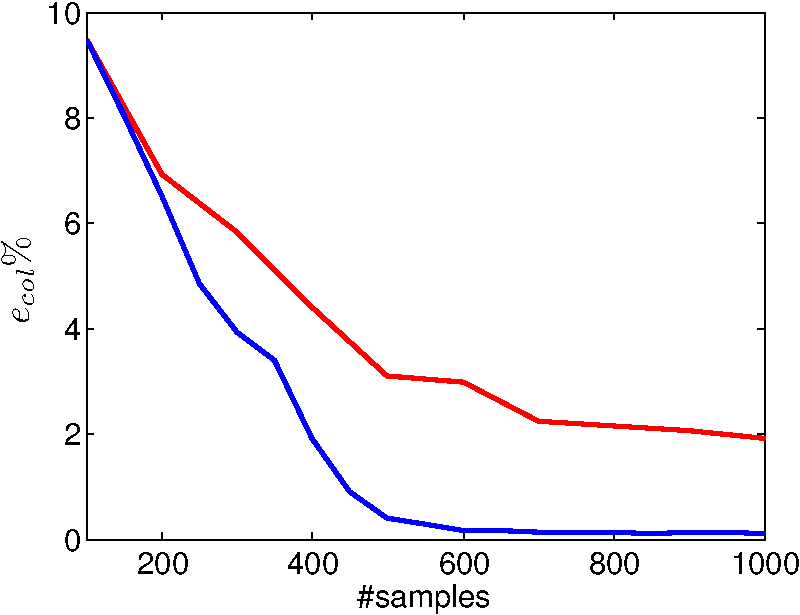
\includegraphics[clip=true, width=0.43\textwidth]{figs/2/active/spider_activelearning-crop.pdf}}
\subfloat[$e_{\text{col}}$ for 3D cup-spoon]{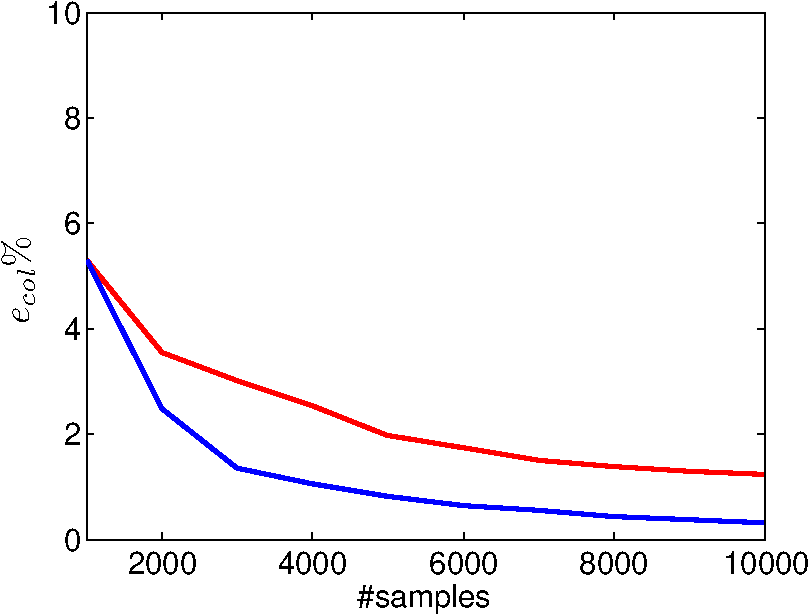
\includegraphics[clip=true, width=0.43\textwidth]{figs/2/active/cupspoon_activelearning-crop.pdf}}
\end{center}
\caption[Relative error convergence of active learning vs. uniform sampling for 2D and 3D object pairs]{Relative error convergence of active learning (blue) vs. uniform sampling (red) for 2D and 3D object pairs. These results demonstrate the benefits of active learning in terms of requiring fewer samples and improved accuracy.}
\label{fig:2:activelearningtime}
\end{figure}

\subsection{Benefits of Active Learning}
A key component of our algorithm is the computation of $\LCS$ by generating appropriate samples in the configuration space. The simplest choice is to perform uniform sampling in $\Cobs (BV(A),BV(B))$ or to use some other random sampling scheme. Instead, we use a combination of active and incremental learning techniques to refine $\LCSi$ and improve its accuracy.


The time and space complexity of the $\LCS$ precomputation phase is a function of
the number of samples used for active learning iterations. The number of samples required to achieve a given error bound $e_{\text{col}}$ depends on both the active learning technique and the underlying classification method used within active learning iterations. It is non-trivial to derive a tight bound on the number of samples required for a specific combination of active learning and classification algorithms. However, we use general results on the sample complexity of active learning~\cite{Hanneke:2013} to show the benefits of our approach.
\begin{theorem}
\label{thm:2:activelearning}
If the number of samples used in active learning iterations of $\LCS$ computation is more than $N$,
where $N=\mathcal O(\log(1/(\epsilon \delta))$, then there exists one active learning technique which can guarantee that with probability at least $1-\delta$, the expected error of the $\LCS$ result will satisfy the bound $e_{\text{col}}\leq\epsilon$.
\end{theorem}

Intuitively, this theorem states there exists a particular active learning technique that will achieve a given bound on $\LCS$ approximation error with high probability.
A proof of this theorem can be obtained based on the CAL (Cohn-Atlas-Ladner) algorithm~\cite{Cohn:ML:1994}. Our $\LCS$ computation is guaranteed to satisfy a bounded error with high probability, if more than $N=\mathcal O(\log(1/(\epsilon \delta))$ samples are used. However, the CAL active learning algorithm is not practical~\cite{Hanneke:2013} and rather we use a combination of exploration and exploitation for active learning (Section~\ref{sec:2:offline:activelearning}) in our $\LCS$ computation algorithm.

Many applications use exploration and exploitation for active learning algorithms. We expect that the use of exploration and exploitation likely also results in a bound similar to Theorem~\ref{thm:2:activelearning}, although the exact derivation of such a bound is a good topic for future research.

Since $e_{\text{col}}$ and $e_{\text{PD}}$ are closely related to each other, Theorem~\ref{thm:2:activelearning} also implies that
$e_{\text{PD}}$ decreases exponentially with the number of samples.
In contrast, when using a uniform sampling strategy to learn the contact space, 
$\LCS$ converges to the
exact contact space
at a polynomial rate as the number of samples
increases~\cite{Mohri:2012:FML}:
\begin{theorem}
\label{thm:2:uniform}
When using uniform sampling, if the number of samples is more than $N$, where $N = \mathcal O(
\frac{1}{2\epsilon^2} \log(2/\delta))$, then
with probability $\geq 1- \delta$, we have the error bound $e_{\text{col}} \leq
\epsilon$.
\end{theorem}

We also measured the expected errors, $e_{\text{col}}$ and $e_{\text{PD}}$, in
complex 2D and 3D benchmarks, as shown in Figure~\ref{fig:2:activelearningtime}.
This demonstrates the high convergence rate and lower error in $\LCS$ computation and PD computation using active learning given the same number
of samples.

\subsection{Benefits of Local Refinement}
Our contact space and PD computation approaches are probabilistic algorithms. Their accuracy is determined by
the samples chosen during the learning phase, including the initial samples and active learning as well as
the runtime queries. As more PD queries are performed within a subspace or a specific region of $\Cspace$,
the accuracy of $\LCS$ in that subspace or region tends to become higher.
This is due to the local refinement step that is performed during runtime whenever we encounter an
inconsistent query configuration.
The incremental learning algorithm updates $\LCS$ around the query configuration by taking into account
local information in $\Cspace$.
In many applications, including dynamic simulation, haptics, or motion planning, a high proportion of
sample queries correspond to positions near the two objects $A$ and $B$. As a result, the runtime
query configurations are relatively close to each other in $\Cspace$ and the local refinement
step improves the accuracy of $\LCS$ in that region. This implies that as more queries are performed in
a localized region of $\Cspace$, the accuracy of $\LCS$ and PD queries improves.
Our algorithm does not make any assumptions about the application or the distribution of runtime query
configurations. We expect that the accuracy of local refinement will improve at the rate given by
uniform sampling (i.e., Theorem~\ref{thm:2:uniform}), rather than at the exponential rate of active learning.
In other words, after generating $N = \mathcal O(1/\epsilon^2)$ samples within a subspace at runtime,
the expected error locally around those samples should be less than $\epsilon$.


\subsection{Time and Space Complexity}
\label{sec:2:analysis:timespacecomplexity}
The precomputation or learning phase is performed for each object pair $(A, B)$
in the environment. The exact collision check is performed using precomputed bounding volume hierarchies.
Given two objects represented as meshes with $m$ and $n$ triangles, the expected cost of a single
exact collision query is $T_{col} = \mathcal O(\log m + \log n)$.

\begin{figure}[!htb]
\begin{center}
\subfloat[$\LCS_0, |S| = 88$]{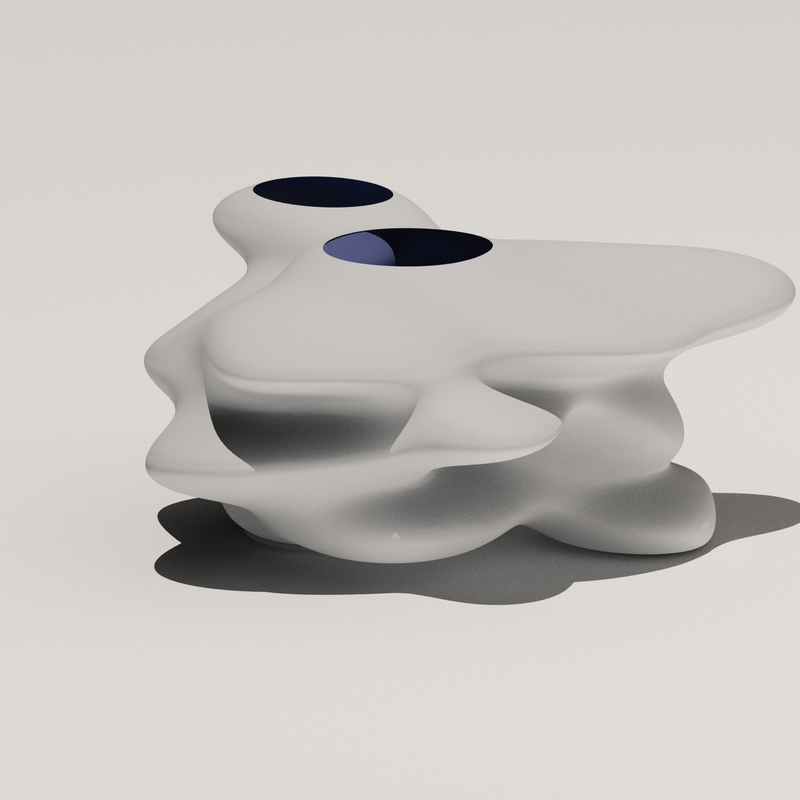
\includegraphics[width=0.24\linewidth]{./figs/2/LCSPDg2D_StarRoom/LCS0.png}}
\subfloat[$\LCS_5, |S| = 174$]{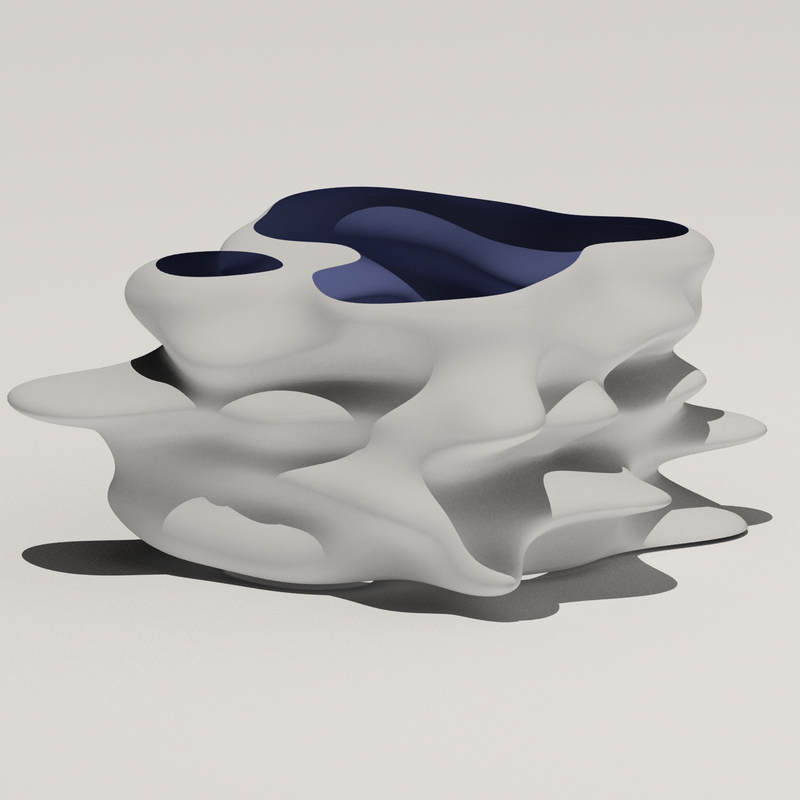
\includegraphics[width=0.24\linewidth]{./figs/2/LCSPDg2D_StarRoom/LCS5.png}}
\subfloat[$\LCS_9, |S| = 237$]{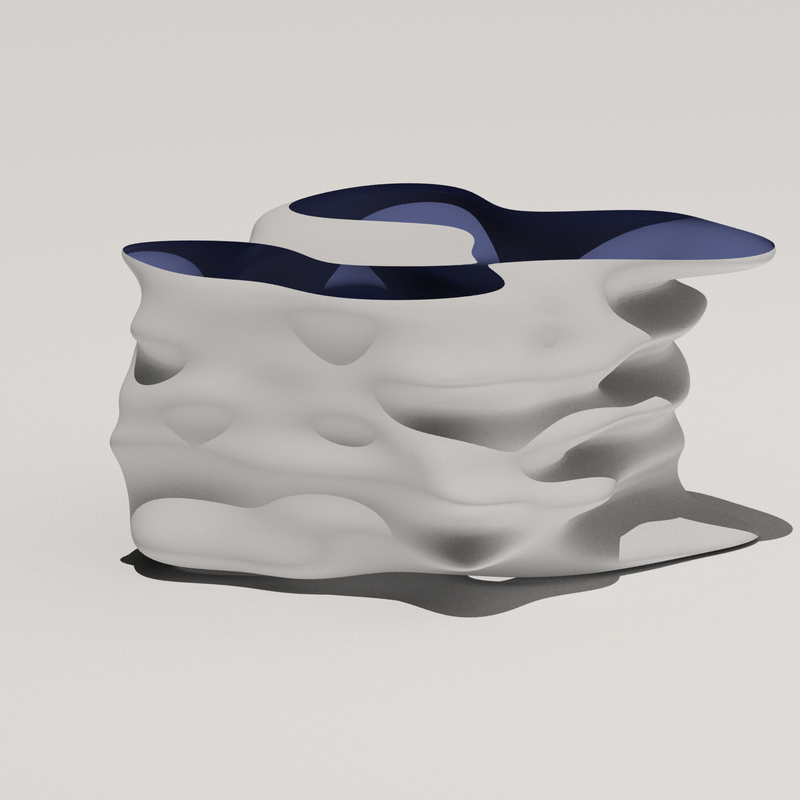
\includegraphics[width=0.24\linewidth]{./figs/2/LCSPDg2D_StarRoom/LCS9.png}}
\subfloat[$\LCS_{12}, |S| = 248$]{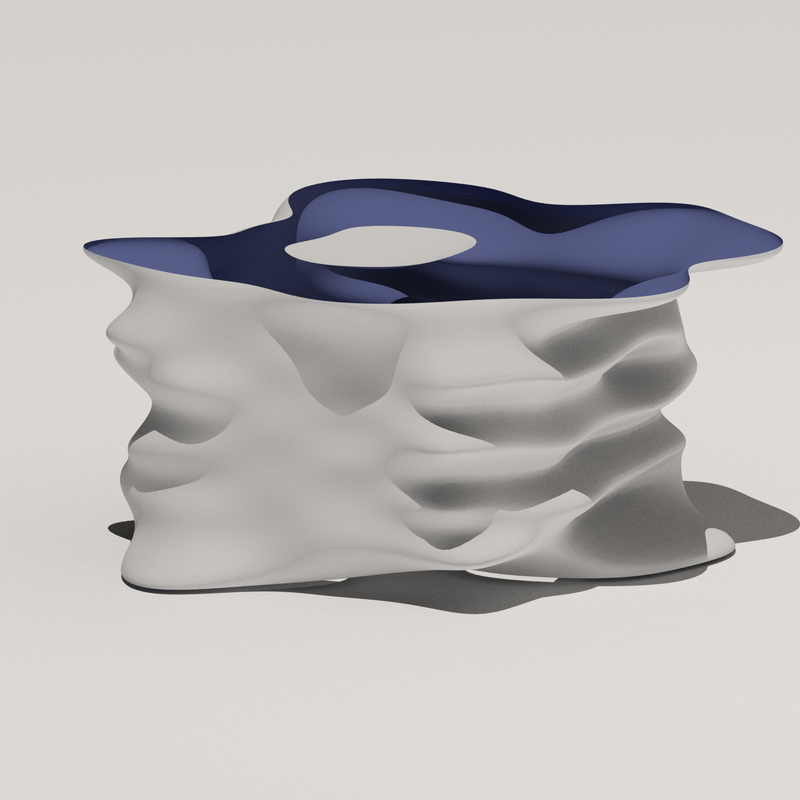
\includegraphics[width=0.24\linewidth]{./figs/2/LCSPDg2D_StarRoom/LCS18.png}}
\caption[$\LCS$ computation using active learning for $\PDg$ query between 2D non-convex shapes]{$\LCS$ computation using active learning for $\PDg$ query between 2D non-convex shapes given in Figure~\ref{fig:2:pipeline}. We show the approximation after $i$-th iteration and the number of support vectors. The vertical axis represents the rotational component of the $\Cspace$. }
\label{fig:2:LCSinActiveLearning2D2}
\end{center}
\end{figure}

\begin{figure}[!htb]
\begin{center}
\subfloat[$\LCS_0, |S|=231$]{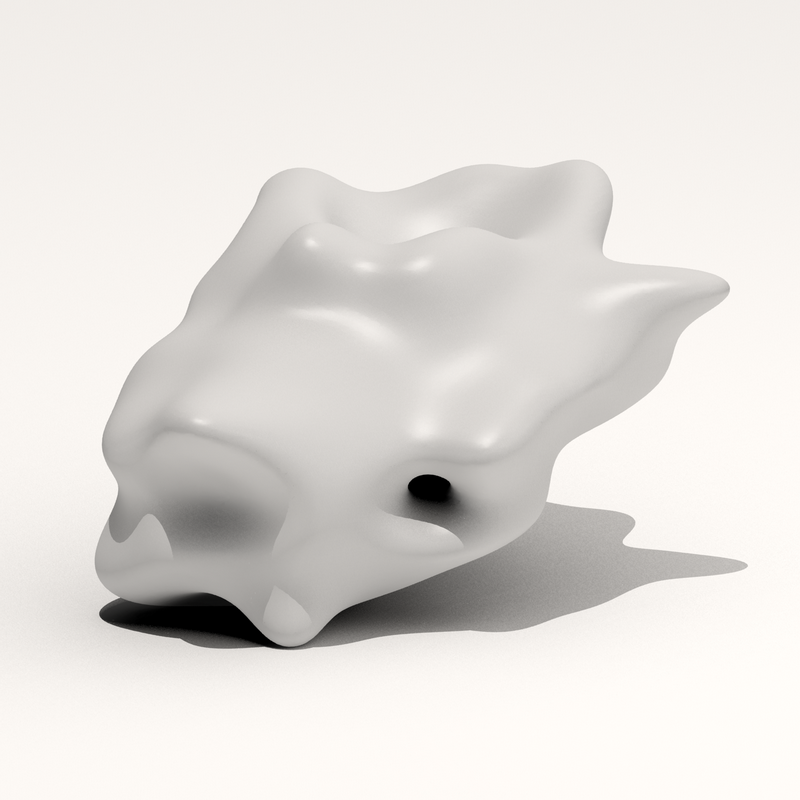
\includegraphics[width=0.24\linewidth]{./figs/2/LCSPDt3D_CupSpoon/LCS0.png}}
\subfloat[$\LCS_5, |S|=869$]{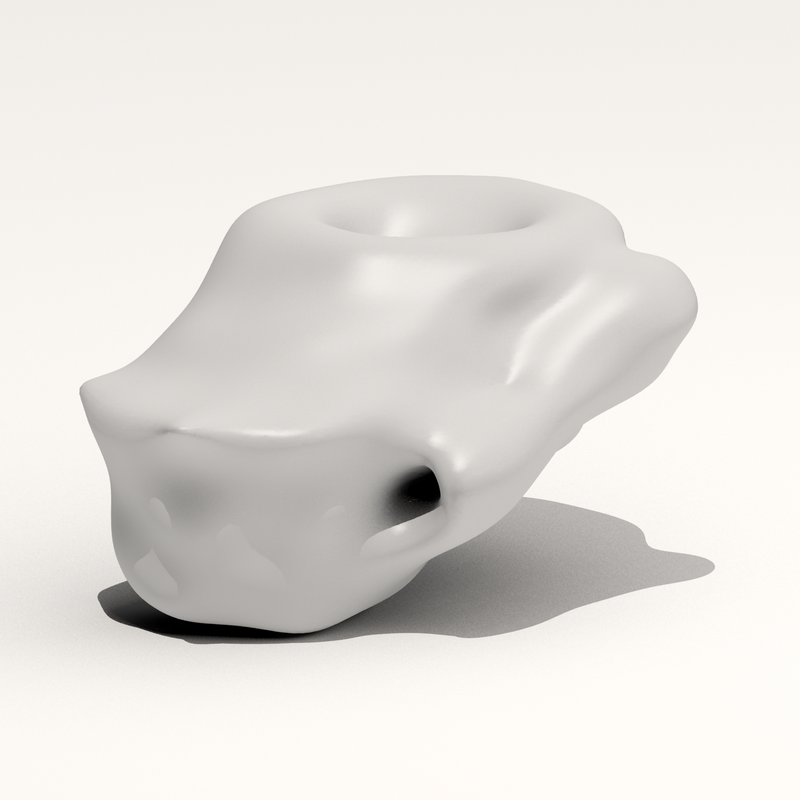
\includegraphics[width=0.24\linewidth]{./figs/2/LCSPDt3D_CupSpoon/LCS5.png}}
\subfloat[$\LCS_9, |S|=1350$]{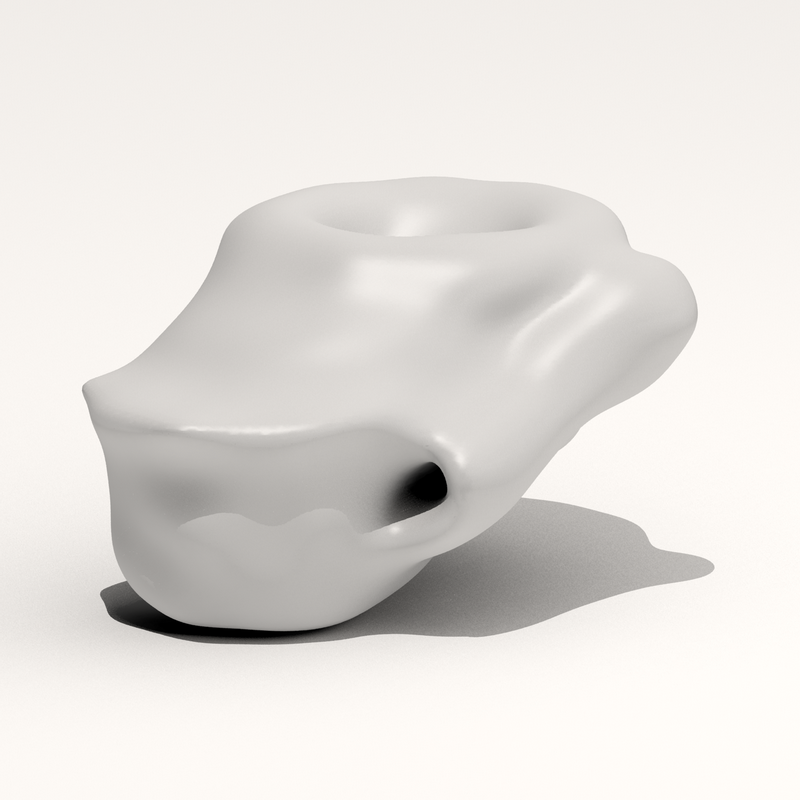
\includegraphics[width=0.24\linewidth]{./figs/2/LCSPDt3D_CupSpoon/LCS10.png}}
\subfloat[$\LCS_{12}, |S|=1572$]{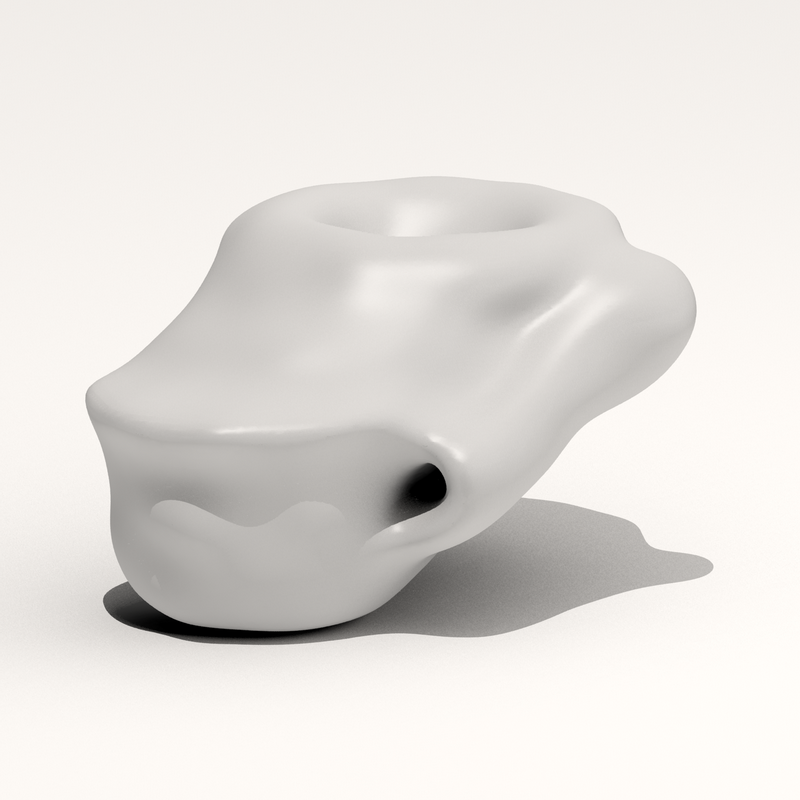
\includegraphics[width=0.24\linewidth]{./figs/2/LCSPDt3D_CupSpoon/LCS17.png}}
\caption[$\LCS$ computation using active learning for $\PDt$ query between 3D cup and spoon]{$\LCS$ computation using active learning for $\PDt$ query between 3D cup and spoon. We provide the number of support vectors corresponding to $\LCSi$. As shown, the algorithm can compute a good approximation in a few iterations.}
\label{fig:2:LCSinActiveLearning3D}
\end{center}
\end{figure}


\paragraph{Offline Learning:} The time complexity for the learning
phase can be estimated as
\begin{align} \label{eq:2:cost}
(T_{LCS_0} + \sum_{i=1}^{I_{AL}} (T_{ES_i} + T_{LCS_i})) + T_{col} \cdot \sum_{i=1}^{I_{AL}} N_{LCS_i},
\end{align}
where $T_{LCS_0}$ is the time complexity to learn the initial approximation;
$T_{ES_i}$ is the time cost to perform exploitation sampling or
exploration sampling in the $i$-th iteration of active learning;
$T_{LCS_i}$ is the time cost for the $i$-th step of incremental
learning, and $I_{AL}$ is the number of iterations performed during active
learning. We denote the number of new samples generated
during $LCS_i$ as $N_{LCS_i}$. We perform collision checking for each sample generated during the learning phase; hence the collision cost is
$T_{col} \cdot \sum_i N_{LCS_i}$.

$T_{LCS_0}$ complexity is governed by the SVM classifier. SVM computation boils down
to solving a constrained quadratic optimization problem using the interior
point or conjugate gradient method, and its worst-case complexity
is $\mathcal O(N_{LCS_0}^{2.3})$.

Incremental learning combines each new sample into $\LCS$ in
constant time, and hence we have $T_{LCS_i} = \mathcal
O(N_{LCS_i})$. $T_{ES_i}$ is the time cost for exploitation sampling
or exploration sampling. For exploration, $T_{ES_i} = \mathcal
O(N_{LCS_i})$. The time complexity for exploitation sampling is
$\mathcal O(|S_{LCS_i}|)$ as we perform interpolation between each
support vector of $\LCSi$ and its $k$-nearest neighbors, which can
be bounded from above as $\mathcal O(\sum_i N_{LCS_i})$.

Overall, the time complexity for the learning phase is
$\mathcal O(\log(\frac{1}{\epsilon}) \sum_i{N_{LCS_i}} +
N_{LCS_0}^{2.3}) + T_{col} \cdot \sum_i N_{LCS_i}$.
The space complexity of our algorithm is linear in the
number of samples used during the learning and runtime phases, and is linear in the number of support vectors in the final $\LCS$ representation.

\paragraph{Runtime Query:} The time complexity in the runtime query
phase depends on $\left| S_{LCS} \right|$, i.e., the number of
support vectors in $\LCS$. $\left| S_{LCS} \right|$ depends on
the smoothness of the exact $\Ccont$, and not as much on the geometric complexity of $A$ and $B$ (see Figures~\ref{fig:2:LCSinActiveLearning2D2} and~\ref{fig:2:LCSinActiveLearning3D}).
For example, the $\Ccont$ of a sphere and another object (i.e., the offset surface) is always smooth, and
therefore a small $\SVLCS$ is sufficient to generate a good approximation of $\Ccont$.
We also notice this in our benchmarks, where $|S|$ for the teeth model (40K triangles) is comparable or higher than that for the bunny (70K triangles), dragon (230K triangles), and Buddha (1M triangles) models. Furthermore, we generated different low-polygon count representations of the Buddha models and observed similar performance on all these approximations.
Thus, the size of
$\SVLCS$ depends on the combinatorial complexity of $\Ccont$ and is also controlled by the tradeoff between 
between the accuracy of PD
computation and the query efficiency.



\section{Implementation and Performance}
\label{sec:2:result}
In this section, we evaluate the performance of our algorithm on complex benchmarks and compare it with prior techniques.
We implemented our algorithm using C++ under Visual Studio 2010
and Windows 7. The two main routines required during the learning phase are exact collision checking between polygonal models and computing the approximate $\LCS$ using support vector machines. At runtime, we need to perform a nearest-neighbor query in the configuration space and to compute a projection using constrained optimization. We used the OBBTree algorithm~\cite{Gottschalk:1996:OHS} for exact collision detection between polygonal objects. We also used a variant of the GJK algorithm~\cite{Gino:2001:GDC} to compute translational penetration depth between convex polytopes, to compare against the performance of our method. In our implementation, we set $\epsilon=2.5\%$ and $\delta=0.01$.

\subsection{Benchmarks}
We have used many complex benchmarks (Figure~\ref{fig:2:demo}) to evaluate the performance of our algorithm. In the simulation, there are multiple contacts between the overlapping objects and we compute $\PDt$ and $\PDg$ between them. The performance of the learning and runtime phases are shown in Table~\ref{tab:2:learningperformance}.

For collision detection, we precompute the BVH for each object, which has a linear memory complexity. For each type of object pair, we precompute the $\LCS$, which takes about 5KB (star-box) to 110KB (teeth, dragon, bunny, Buddha) memory.





\subsection{Physically-based Simulation using PD}
Penetration depth has been used in many dynamic simulators to compute collision response based on penalty forces or constraint-based solvers.
We have integrated our new PD algorithm into two well-known game physics
engines: Box2D~\cite{Erin:2012:Box2D} and Bullet~\cite{Erwin:2012:Bullet}. These engines have support for PD computation based on
convex decomposition and can compute the local translational penetration depth between convex polytopes~\cite{Gino:2001:GDC}.
However, convex decomposition can result in a high number of convex pieces, Moreover, the decomposition-based approach is mainly limited to closed
objects and does not guarantee that two
overlapping non-convex objects will separate, as they only compute local PD using the convex pairs.

\textbf{Contact Points and Normals:} For an inter-penetration configuration $\qa$ and its resulting contact configuration $\qc$, the contact points and contact normal can be computed in the workspace for two objects. First, for the contact configuration $\qc$, its nearest collision-free configuration can be computed using support vectors based on $k$-nearest neighbor search in $\Cspace$. Next, the closest points and normals of the given two objects can be computed using the proximity query algorithm~\cite{LGLM00}. Reliable multiple contact points can be obtained using perturbation and persistent contact caching techniques~\cite{Erwin:2012:Bullet}.

\textbf{Box2D} uses PD computation in the impulse-based collision response algorithm.
We demonstrate the performance of our algorithm on
two complex benchmarks (Figure~\ref{fig:2:demo}): (1) angry bird characters falling into a complex chute and (2) Nazca spiders rolling in a tumbler. We precompute the $\LCS$ approximation for a 3-DOF $\Cspace$.
The convex decomposition results in $17$, $30$, and $32$ convex pieces for the BigRedBird, WhiteBird and GreenPig models, respectively. The Nazca spider is decomposed into $77$ convex pieces. We observed an improvement in PD querying of nearly a factor of $20$ when using our active learning algorithm, compared to
techniques based on convex decomposition used in Box2D (see Figure~\ref{fig:2:performancecomparison}(a)(b)). The collision response algorithm is based on the Box2D implementation.


\textbf{Bullet} uses PD computation to handle penetrations in their constraint-based solver.
We demonstrate the benefits of our PD computation algorithm in three scenarios (shown in Figure~\ref{fig:2:demo}):
(1) interlocking $10$ rings; (2) a rainfall of $1,000$ rings; and (3) collapse of a tower composed of $5,500$ rings.
Each ring consists of $256$ triangles and is decomposed into $16$ convex pieces for convex-decomposition.
We precompute the $\LCS$ approximation for a 6-DOF $\Cspace$ and use the approximate result to perform PD queries during the simulation.
Compared to the convex decomposition based algorithm used in Bullet, our PD computation algorithm is about
an order of magnitude faster. We use the standard implementation of contact normal and collision response forces computation available in Bullet.

\textbf{Complex 3D Models}:
We evaluated the performance of our algorithm on many complex models corresponding to the cup-spoon, moving teeth, bunnies, dragons, and Buddha models (Figure~\ref{fig:2:demo}) where we performed $\LCS$ computation for the 6D $\Cspace$. We observed more than an order of magnitude performance improvement compared to prior methods.


\begin{figure}[!h]
  \centering
  \subfloat[$\PDg$: cup-spoon]{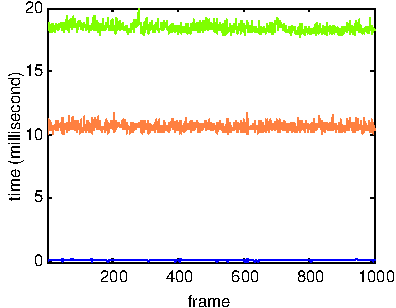
\includegraphics[width=0.49\linewidth]{figs/2/comparison/cupspoon-crop.pdf}}  \hspace{0.05em}
  \subfloat[$\PDg$: rings (Bullet)]{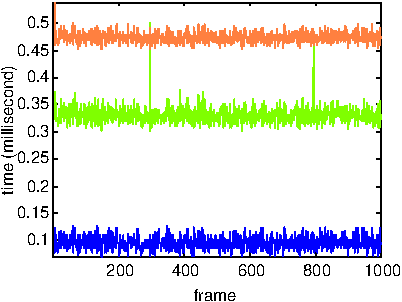
\includegraphics[width=0.49\linewidth]{figs/2/comparison/ring-crop.pdf}}
  \caption[Relative performance of PD computation for different benchmarks]{Relative performance of PD computation for different benchmarks: The blue curve represents the query time computed by our approximate $\PDg$ algorithm. The green curve corresponds to the query time computed using convex decomposition and local PD between convex pairs. The orange curve represents the $\PDg$ query time computed using point-based approximation~\protect\cite{Lien:2009:ASM}.}\label{fig:2:performancecomparison}
\end{figure}



\begin{figure}[!htb]
  \centering
  \subfloat[]{\includegraphics[width=0.49\linewidth, page=4]{figs/2/comparison/PD_bunny_bunny.pdf}}
  \subfloat[]{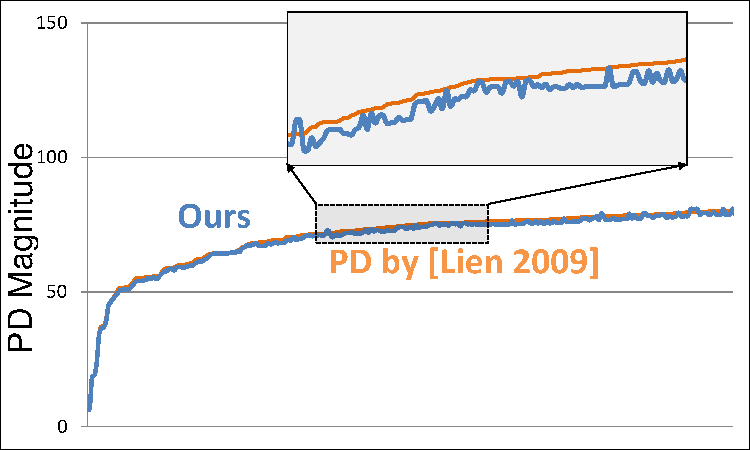
\includegraphics[width=0.49\linewidth, page=1]{figs/2/comparison/PD_bunny_bunny.pdf}}\\
  \subfloat[]{\includegraphics[width=0.49\linewidth, page=2]{figs/2/comparison/PD_bunny_bunny.pdf}}
  \subfloat[]{\includegraphics[width=0.49\linewidth, page=3]{figs/2/comparison/PD_bunny_bunny.pdf}}
  \caption[The performance and accuracy compared to PolyDepth on bunny-bunny benchmark]{The performance and accuracy compared to PolyDepth~\protect\cite{Je:2012:PRP} on the bunny-bunny benchmark. (a) computational time (on average, 0.10ms based on our algorithm vs. 7.15ms in PolyDepth); (b) accuracy comparison between our interactive algorithm vs. an offline algorithm based on Minkowski sum~\protect\cite{Lien:2009:ASM}; (c) accuracy comparison of PD computation between our algorithm vs. PolyDepth; (d) our global PD algorithm (blue) has lower error compared to PolyDepth, which performs local optimization. }\label{fig:2:bunnymodels}
\end{figure}

\begin{figure}[!htb]
  \centering
  \subfloat[]{\includegraphics[width=0.49\linewidth, page=4]{figs/2/comparison/PD_dragon_dragon.pdf}}
  \subfloat[]{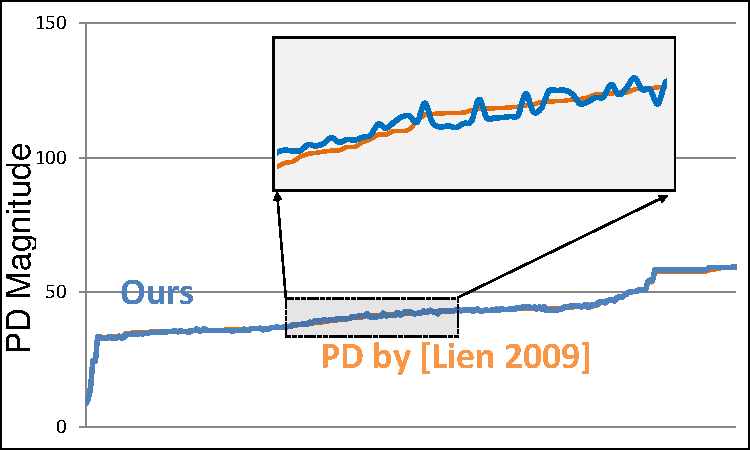
\includegraphics[width=0.49\linewidth, page=1]{figs/2/comparison/PD_dragon_dragon.pdf}}\\
  \subfloat[]{\includegraphics[width=0.49\linewidth, page=2]{figs/2/comparison/PD_dragon_dragon.pdf}}
  \subfloat[]{\includegraphics[width=0.49\linewidth, page=3]{figs/2/comparison/PD_dragon_dragon.pdf}}
  \caption[The performance and accuracy compared to PolyDepth on dragon-dragon benchmark]{The performance and accuracy compared to PolyDepth~\protect\cite{Je:2012:PRP} on the dragon-dragon benchmark. (a) computational time (on average, 0.12ms based on our algorithm vs. 9.86ms in PolyDepth); (b) accuracy comparison between our interactive algorithm vs. an offline algorithm based on Minkowski sum~\protect\cite{Lien:2009:ASM}; (c) accuracy comparison of PD computation between our algorithm vs. PolyDepth; (d) our global PD algorithm (blue) has lower error compared to PolyDepth, which performs local optimization.}\label{fig:2:dragonmodels}
\end{figure}



\subsection{Comparison with Prior Methods}
Most existing practical algorithms perform local analysis of the intersection regions and
compute local PD. Other techniques use distance fields and can be accelerated using GPUs. In practice, these techniques are quite fast and can also handle
deformable models. On the other hand, our global PD algorithm involves preprocessing and is mainly designed for rigid objects.
The performance of our runtime query (e.g., about $0.1\sim2$ milliseconds) is comparable to or faster than these local PD computation algorithms. The main benefit of our approach over local PD methods is the computation of global
translational and rotational PD, which provides a more reliable measure of separating two overlapping objects.
Other algorithms reduce PD computation to constrained optimization~\cite{Nawratil:2009:GPD,Zhang:2007:AFP,Je:2012:PRP,Tang:IGP:2013}.
In these techniques, a sequence of configuration samples on the contact space are iteratively
computed until a local minimum configuration is found. The
performance of these algorithms heavily relies on the initial guess of the configuration, and it is hard to provide
error bounds in terms of global PD (see Figure~\ref{fig:2:bunnymodels} and~\ref{fig:2:dragonmodels}). 
However, compared to our method, the optimization-based algorithms have several advantages. First, they require no pre-computation and can be applied to environments with many different obstacles. Our method's dependence on pre-computation limits its application.
Moreover, for generalized PD computation involving rotations, optimization-based algorithms such as~\cite{Tang:IGP:2013} may provide better results than our method, especially for queries with small penetration depths. This is due to our method's essential limitations related with 
the use of sampling-based approaches and the design of configuration space metrics (more details in Section~\ref{sec:2:limitations}).
Our approximate PD algorithm may be used as a complimentary approach to the optimization-based local approaches. The approximate PD computed by our global algorithm can be used as an initial guess for these optimization-based techniques and thereby improve their accuracy, while also keeping the high efficiency of our method.


In order to evaluate the error in our approximate PD computation algorithm, we need to compute the ground truth for the PD value between two objects. For translational PD, the ground truth PD can be obtained by computing the Minkowski sum between two objects. 
It is difficult to compute exact Minkowski sum for complex 3D objects like the teeth or dragon, due to the combinatorial complexity arises. Instead we use the point-based algorithm~\cite{Lien:2009:ASM} to approximate the PD and estimate the error of our algorithm.
For generalized PD, the ground truth PD computation is even harder. Therefore, we approximate the exact contact space with many slices of Minkowski sums. Intuitively, we sample many rotations in rotation space and then compute Minkowski sums for all the rotations. The combination of these Minkowski sums is used as an approximation of the contact space. We label the PD computed using these offline techniques as "\emph{nearly exact PD}" for our algorithm and comparisons.
In practice, our approach is more than an order of magnitude faster than other algorithms that are based on convex decomposition (e.g., \cite{Kim:2002:FPD} for $\PDt$; \cite{Zhang:2007:GPD} for $\PDg$) or point-based approximations. We have compared the runtime performance of our algorithm with these prior global methods in Figure~\ref{fig:2:performancecomparison}. More benchmarks, results, and comparisons are given in the supplementary material.


\section{Limitations}
\label{sec:2:limitations}
Our approach is the first attempt at using machine learning techniques to improve the performance and accuracy of penetration depth computation. In order to make this method useful for real-world applications, certain limitations need to be addressed in the future. In our discussion, we divide these limitations into two categories: limitations related to approximate configuration space computation, and limitations related to approximate penetration depth computation. 

\subsection{Limitations Related with Approximate Configuration Space Computation}
The first limitation related with approximate configuration space computation is that the precomputation phase must be performed for each pair of moving objects in the simulation. Thus, in the worst case, its complexity grows as a quadratic function of the number of objects in the simulation. In addition, the accuracy and running time of our learning phase is a function of the combinatorial complexity of the contact
space and the sampling scheme. Hence, it is possible that our method may not generate a sufficient number of samples in small,
isolated components of contact space, or it may take a large number of iterations.
Moreover, the overall approach is probabilistic, and all of our error bounds are derived in terms of expected error.

\subsubsection{Degenerate Geometric Representation}
In Section~\ref{sec:2:intro}, we claimed that our method is general and is able to compute the contact space for complex non-convex and non-manifold models. However, this claim is based on the implicit assumption that a `correct' collision detection routine is available for input geometric data; the `correctness' means that the collision result provided by the collision checking routine can correctly reflect objects' collision status in physical world. Whether this assumption holds will determine the correctness of the contact space computed by our learning framework. For example, if objects are represented as meshes, the assumption generally holds even if input meshes are non-convex, non-manifold, or not-closed. Thus, our method usually can return a correct approximate contact space. However, the assumption may not hold for meshes in several degenerate cases. First, suppose that we are given two objects represented as mesh soups (i.e., without the connectivity information between mesh triangles). If these two objects are so different in scale that one object $A$ can be completely contained inside the other object $B$, the mesh-mesh collision checking will always report collision-free for configurations in which $A$ locates inside $B$, while in physical world $A$ and $B$ should be in-collision. Thus, our learning framework will not provide a correct contact space in this case. Indeed, there exist advanced algorithms such as~\cite{Ju:2004:RRP} that can recover or estimate objects' volumetric information from mesh soups, but these algorithms are non-trivial to implement. Second, if the mesh representation of object $B$ has a hole larger than the size of object $A$ (Figure~\ref{fig:2:hole}), the collision checking will also give incorrect results and our learning framework will fail to compute a reasonable contact space. There are several possible solutions to this limitation, including 1) designing better collision checking routines for these degenerate cases; and 2) using the solid geometry instead of meshes to represent objects.

\begin{figure}[!htb]
  \centering
  \subfloat[]{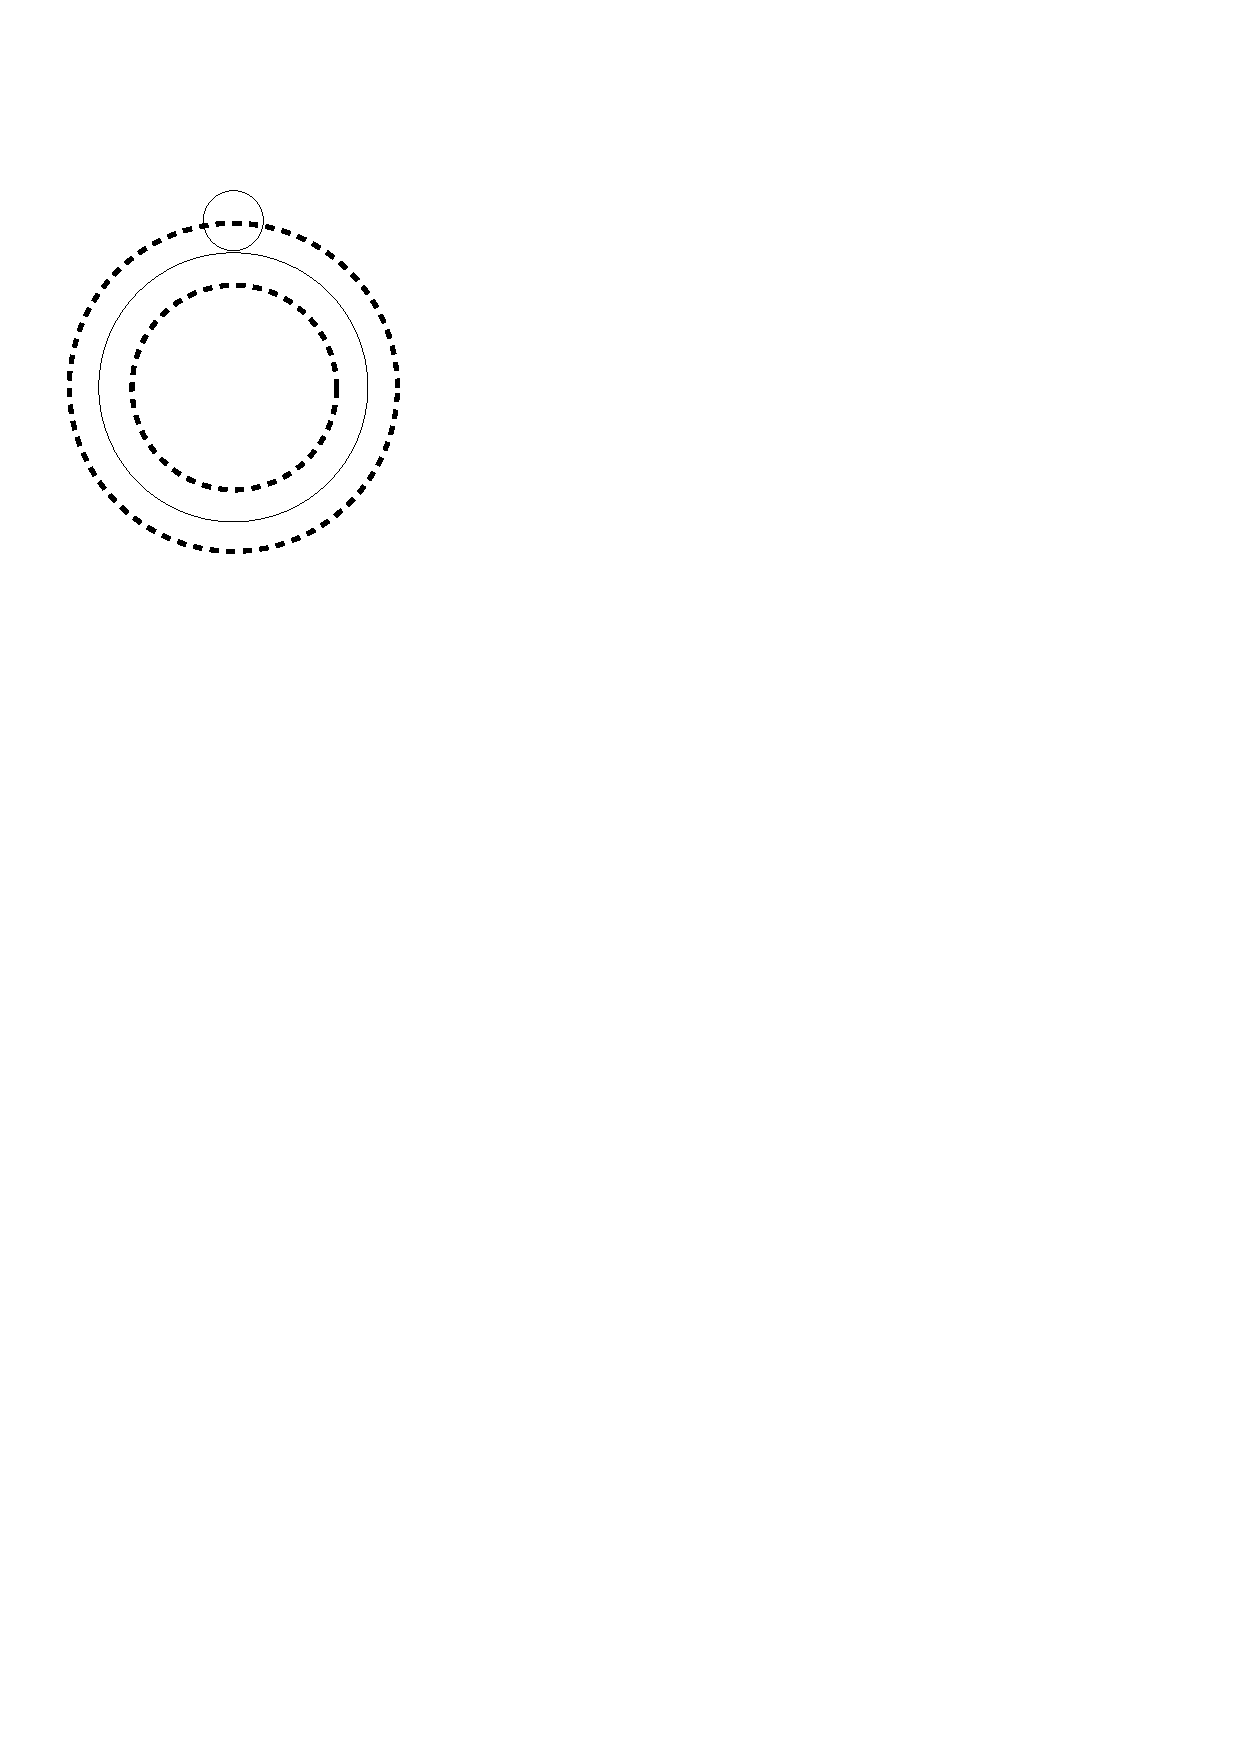
\includegraphics[width=0.3\linewidth]{figs/2/hole1.pdf}}
  \subfloat[]{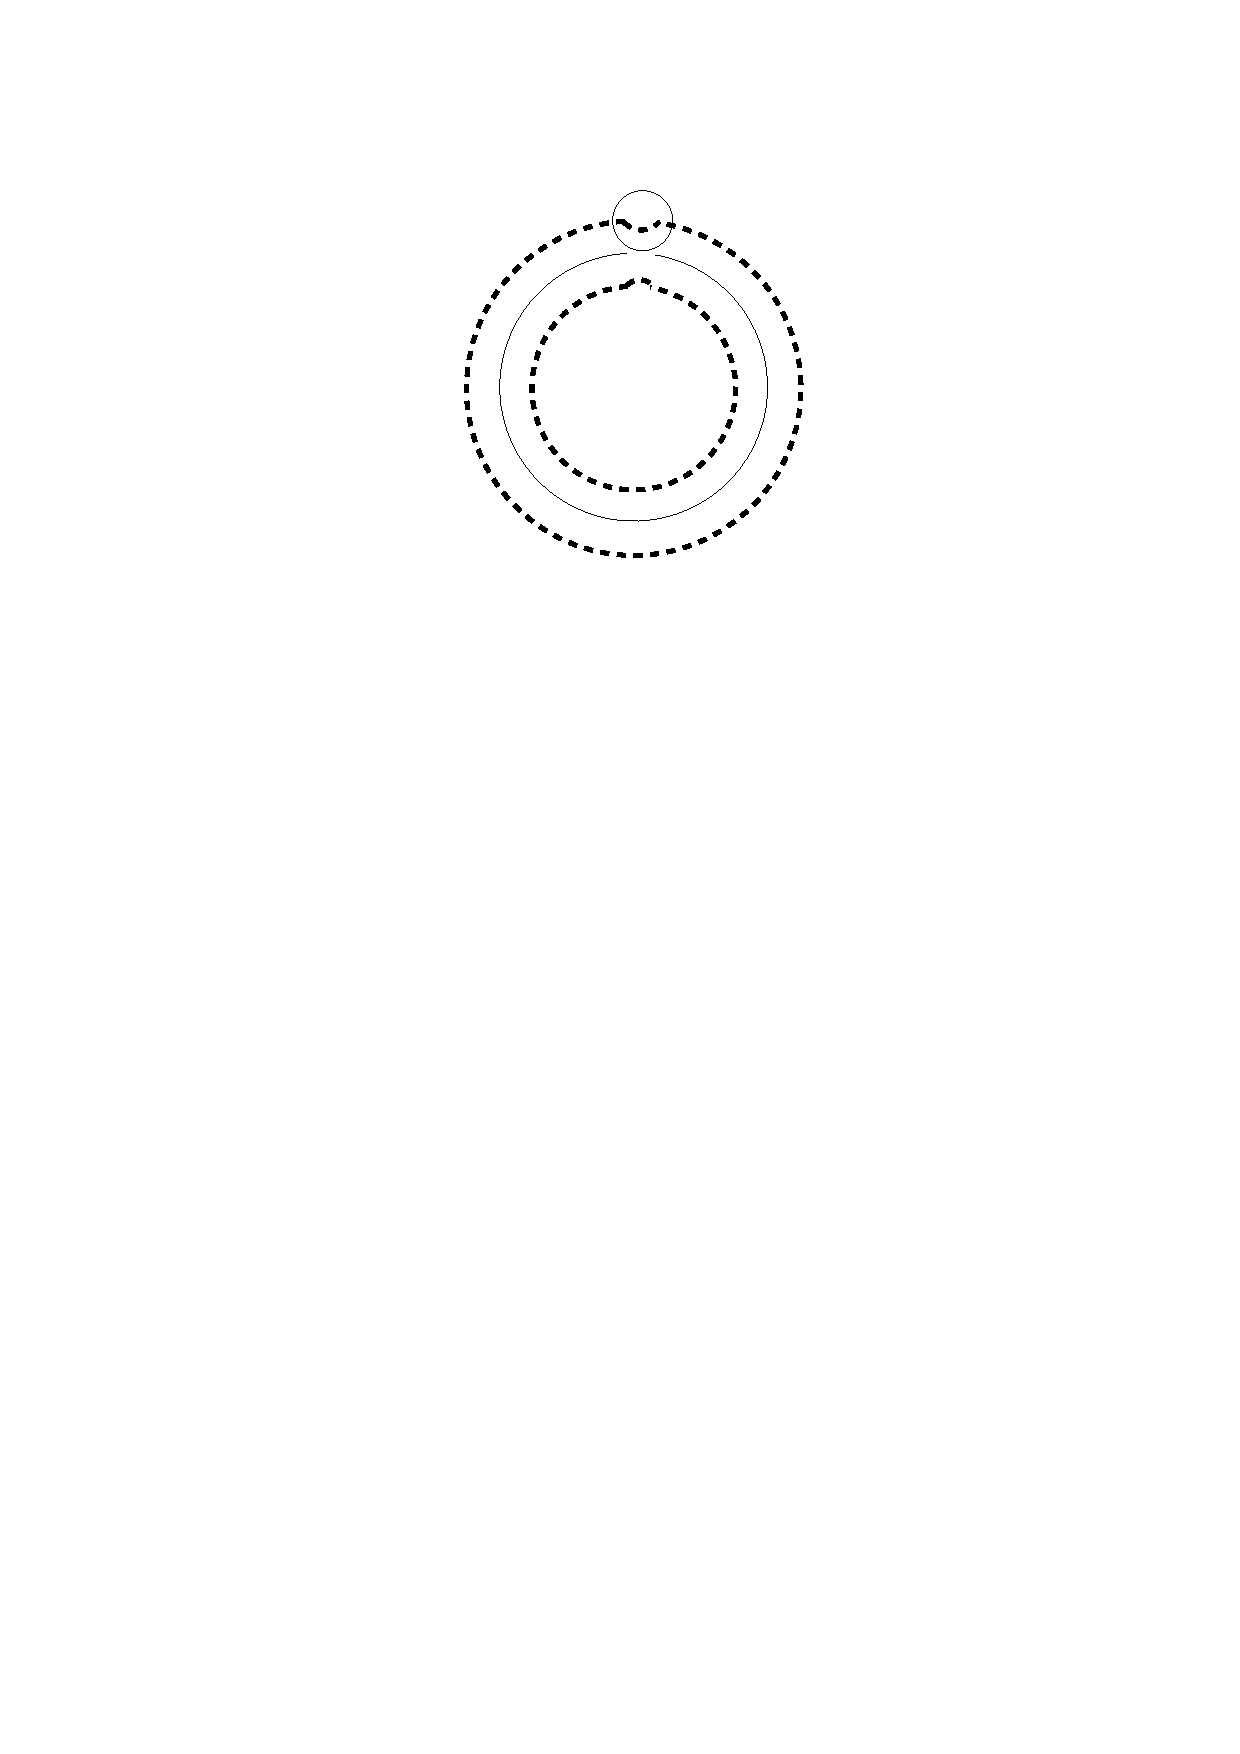
\includegraphics[width=0.3\linewidth]{figs/2/hole2.pdf}}
  \subfloat[]{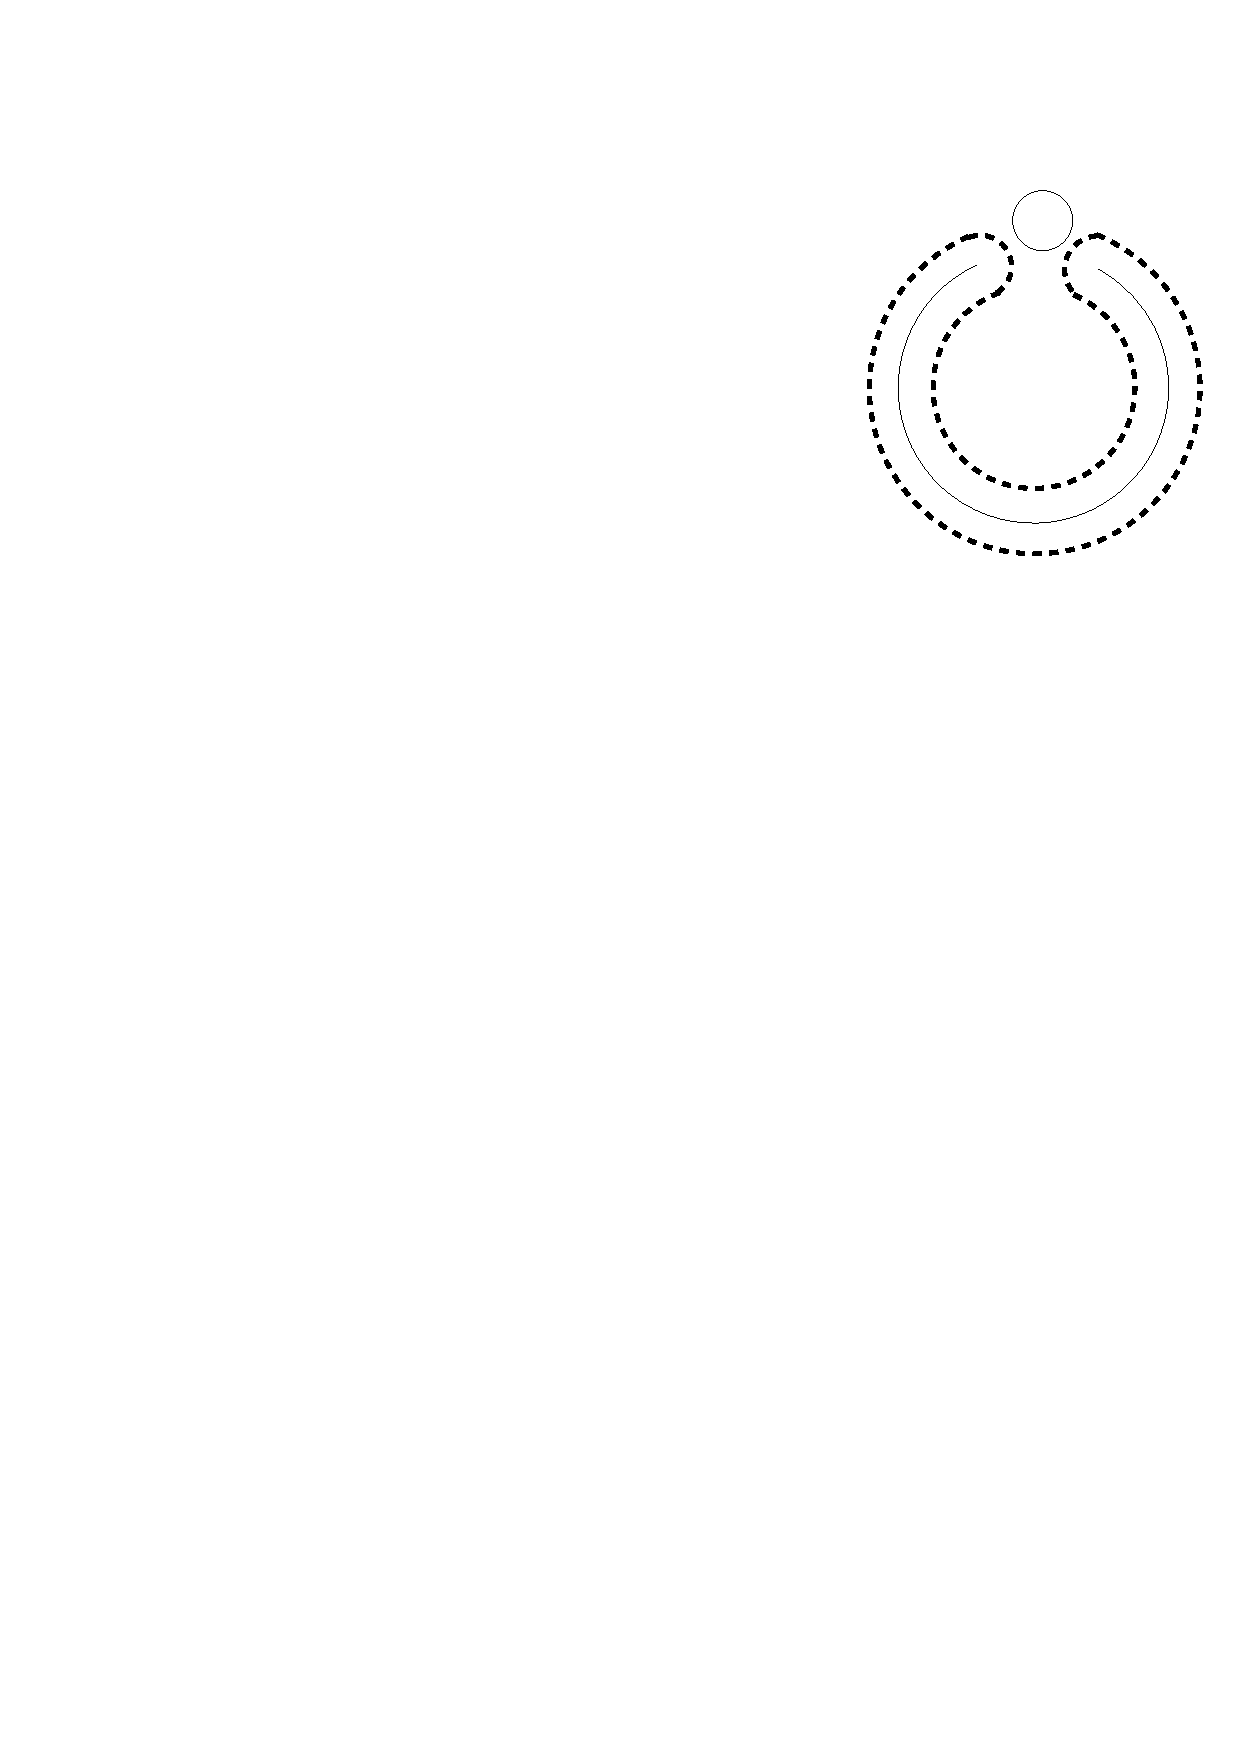
\includegraphics[width=0.3\linewidth]{figs/2/hole3.pdf}}
  \caption[One example for the degenerate case of configuration space computation]{One example for the degenerate case of configuration space computation.
We are given two objects, one large circle and one small circle. (a) The geometric representations of the objects are exact and the contact space is shown as a dashed circle. (b) The big circle has a small hole and the contact space (the dashed curve) is slightly different with the exact contact space in (a). (c) The big circle has a large hole and the contact space (the dashed curve) is completely different with the exact contact space in (a). In many applications, the geometric representation of objects have hole artifacts, which may result in low quality contact space similar to (c). 
}\label{fig:2:hole}
\end{figure}


\subsubsection{SVM Implementation}
When describing the learning framework in Section~\ref{sec:2:offline:svm}, we use the hard-margin SVM (Equation~\ref{eq:2:svm1}) to introduce the main idea of our algorithm, since all in-collision samples and collision-free samples are separable. However, in implementation we use the soft-margin SVM defined as follows:
\begin{align}
\label{eq:2:svmsoft}
& \underset{\mathbf w, b, \xi}{\text{min}} & & \frac{1}{2}\|\mathbf w\|^2 + C \sum_{i=1}^k \xi_i & &  \\
& \text{subject to} & & c_i (\mathbf w \cdot \phi(\mathbf q_i) + b)
\geq 1 - \xi_i, & & \xi_i \geq 0 & & 1 \leq i \leq k. \notag
\end{align}
In soft-margin SVM, slack variables $\xi_i$ measure the degree of misclassification of the data; the objective function is increased by a term which uses a weight variable $C$ to penalize non-zero $\xi_i$. The optimization becomes a trade-off between a large margin and a small error penalty. 

In practice, a soft-margin SVM behaves better than a hard-margin SVM, even when data is separable, as it happened in our case. The reason is that for a hard-margin SVM, a single outlier (e.g., a sample extremely close to the actual contact space) can determine the boundary, which makes the classifier overly sensitive to the data. For contact space learning, a hard-margin SVM will generate an uneven contact space with jagged edges, while the soft-margin SVM can provide a smooth contact space. 

However, the soft-margin SVM needs to select an appropriate penalty weight $C$, which is not an easy task. A suitable value of $C$ is related with the set of samples used to learn a contact space; it is also related with the number of samples used. A small value of $C$ will result in a large error in the approximate contact space, while a large $C$ will result in a non-smooth contact space or a contact space approximation with incorrect topology. Theoretically, cross-validation provides a systematic manner for choosing $C$, but it is computationally expensive. In our experiments, we run the learning algorithms with different $C$ values and select the $C$ which generates the approximate configuration space with the smallest error. 

\subsubsection{Learning on Non-Euclidean Structure}
When learning a contact space in $\SEcubic$, we simply convert every configuration into a vector in the Euclidean space: for the rotation component of each configuration, we either convert it into a $3$-dimensional vector corresponding to the Euler angles or into a $4$-dimensional vector corresponding to a quaternion. Given the vector representation of each configuration, we then perform the learning algorithm directly in the Euclidean space. However, $\SEcubic$ in fact is a Lie group and the Euclidean space approximation is only valid locally around each configuration. More formally, the Euclidean space locally approximates the Lie algebra element $\exp(\mathbf q)$ of a given configuration $\mathbf q \in \SEcubic$, where $\exp$ is the exponential map from $\SEcubic$ to its corresponding Lie algebra $se(3)$~\cite{Murray:1994:MIR}. Our current method does not consider additional constraints and structures from the underlying Lie group and thus may not provide good results for contact spaces with significant rotation components. One possible solution to this limitation is using learning algorithms on Lie groups~\cite{Tuzel:2008:LLG}.

The difficulty of non-Euclidean structure arises because our method aims at computing a global representation for the contact space, i.e., the representation is valid and accurate for any points in the contact space. An accurate global representation is challenging because it is not difficult to have an Euclidean space globally approximate a non-Euclidean space while also preserving the distance metric. However, it is still possible to provide a Euclidean approximation with high accuracy to a non-Euclidean space locally around a configuration. This approximation strategy is widely-used in optimization-based local PD algorithms such as~\cite{Nawratil:2009:GPD,Zhang:2007:AFP,Je:2012:PRP,Tang:IGP:2013}, in which different heuristics are applied to approximate the contact space locally around an in-contact configuration. The local approximation of the contact space is easier to compute than the global contact space. However, the global contact space is only computed once during the pre-computation step and can be reused during online PD queries. In other words, compared to the local contact space approximation used in previous PD algorithms, our method tries to solve a more challenging problem and attempts to compute a global approximation of the contact space. 


\subsection{Limitations Related with Approximate Penetration Depth Computation}

\subsubsection{Penetration Depth Formulation}

First, the solution to the penetration depth problem (Section~\ref{sec:2:overview:pdformulation}) is often not unique or differentiable. Since we compute a bounded-error approximation of PD, there could be multiple solutions that satisfy those error bounds. This discontinuity in PD formulation and computation can cause instability in collision response for haptic rendering. In complex rigid-body simulations with multiple objects, global PD computation can improve the accuracy of the simulation, but cannot guarantee that it is totally collision-free.

Second, the penetration depth definition used in our method (Equation~\ref{eq:2:PDgdef}) is a pure geometric definition. In particular, the penetration depth is completely determined, given two objects and their configurations, and is independent with objects' velocity and acceleration. Due to this property of our PD definition, the PD result provided by our method may not be suitable for some applications. For instance, many physically-based simulation algorithms use PD values to estimate the reaction forces and torques between objects. Since the reaction forces and torques are related to the relative velocity and acceleration between objects, our method cannot provide the correct PD values for force and torque computations. 

\subsubsection{Configuration Space Metric}
The penetration depth formulation in Equation~\ref{eq:2:PDgdef} requires a suitable metric to be defined over the entire configuration space. Given any two points in the configuration space, this metric should correctly measure the distance or difference between them.  
For $\PDt$, we can simply use the Euclidean metric since the underlying configuration space is a Euclidean space. 
For $\PDg$, the configuration space is non-Euclidean and hence the metric selection is more challenging. For a specific application, how to define a good metric in $\SEcubic$ is the main challenge when applying our learning-based framework. 


We currently use the metric defined in Equation~\ref{eq:PDgmetric}, which uses weights $\mu_1$, $\mu_2$ and $\mu_3$ to balance the relative weight between the rotational component and the translational component. This metric has several issues. 

First, this metric only involves the geometric information of the moving object $A$ and is not related with the geometric information of the fixed object $B$. As a result, this metric cannot handle the cases where both objects are moving. One possible solution is using $0.5(\dist_{A}(\mathbf q_i, \mathbf q_j) + \dist_{B}(\mathbf q_i, \mathbf q_j))$, where $\dist_{A}$ and $\dist_{B}$ denote the metric whose parameters are computed based on object $A$ and object $B$, respectively. However, while $\dist_{A}(\mathbf q_i, \mathbf q_j)$ measures the energy required to move $A$ from $\mathbf q_i$ to $\mathbf q_j$, the new metric no longer has such physical meaning.

The second problem about this metric is related with our approach's use of sampling-based techniques. During the off-line learning phase, we only generate a limited number of samples in the configuration space; these samples are used to compute the approximate configuration space. During run-time, a given in-collision query $\mathbf q_0$ is projected onto the set of these discrete samples via the nearest-neighbor algorithm, to obtain the corresponding in-contact configuration $\mathbf q_c$. If $\mu_i$ is large, we assign a large penalty to configurations' difference in the rotational component, and thus $\mathbf q_0$ and $\mathbf q_c$ will have a small difference in the rotational component. Theoretically, if $\mu_i \rightarrow \infty$, we can use $\PDg$ to compute $\PDt$. However, this is not feasible in practice, due to the use of sampling-based techniques in our method. Among all the pre-computed samples in the configuration space, there may be no samples with the same rotational component as the query configuration $\mathbf q_0$. Thus, our sampling-based framework can only provide an in-contact configuration whose rotational component is close to that of $\mathbf q_0$, but not exactly the same.

The use of sampling-based techniques also results in the discontinuity of PD values. Suppose the moving object is collision-free in the beginning; at the next instance, it is in contact with the obstacles, and finally collides with some obstacles. Intuitively, the PD value should be zero when contact occurs and then increase continuously. However, since there are only limited number of configuration samples in the approximate contact space, usually we cannot find a sample exactly the same as the in-contact query. Under a given PD metric, the in-contact sample closest to the query always has a non-zero distance to the query, no matter how many samples are generated for approximating the contact space (because the measure of a limited number of samples is zero in the continuous configuration space). As a result, the approximate PD for a given query will suddenly ``jump'' from zero toward non-zero; such jump may not be acceptable in many applications. To avoid this artifact, we need to perform continuous search around the in-contact candidate configuration provided by our approximate PD method. One option for the continuous search is an optimization-based local PD algorithm such as~\cite{Tang:IGP:2013}, which can eventually report a zero PD value for an in-contact query.

The selection of $\mu_i$ in the metric formulation will greatly influence final PD values. Large $\mu_i$ will result in high vibrations in the PD values, especially when the moving object is rotating. This is because metric parameters $\mu_i$ are the metric function's derivatives with respect to the rotational component, and thus large $\mu_i$ will make the nearest-neighbor algorithm highly sensitive to the change in the query's rotational component. As a result, a slight rotation of the moving object $A$ will result in a large change in the PD value. Large $\mu_i$ will also cause other problems. For instance, suppose we are given a query configuration with a small penetration. Intuitively, the PD algorithm should return an in-contact sample which has a translational component similar to the query and with an appropriate rotational component. However, due to the limited number of samples for approximating the contact space, it is possible that all the samples closest to the query in translation have a larger rotational difference with the query, than one sample $\mathbf q_{bad}$ that is far away from the query in translation. For large $\mu_i$, the difference in rotational component dominates the distance between the query and other samples, especially for a query with a small penetration. As a result, $\mathbf q_{bad}$ will be the in-contact sample reported by our PD method, though it is not a suitable result. Such inaccuracy is smaller for a query with a deep penetration, because the translational difference makes a larger component of the PD measurement for queries with deeper penetrations. Similar inaccuracies will arise when the weights $\mu_i$ are too small. For instance, there may be high vibrations in PD values when the moving object is translating. Moreover, small $\mu_i$ may result in a large rotation difference between the query configuration and the in-contact configuration computed by the PD algorithm.

\begin{figure}[!h]
\centering
\subfloat[Rotation movement]{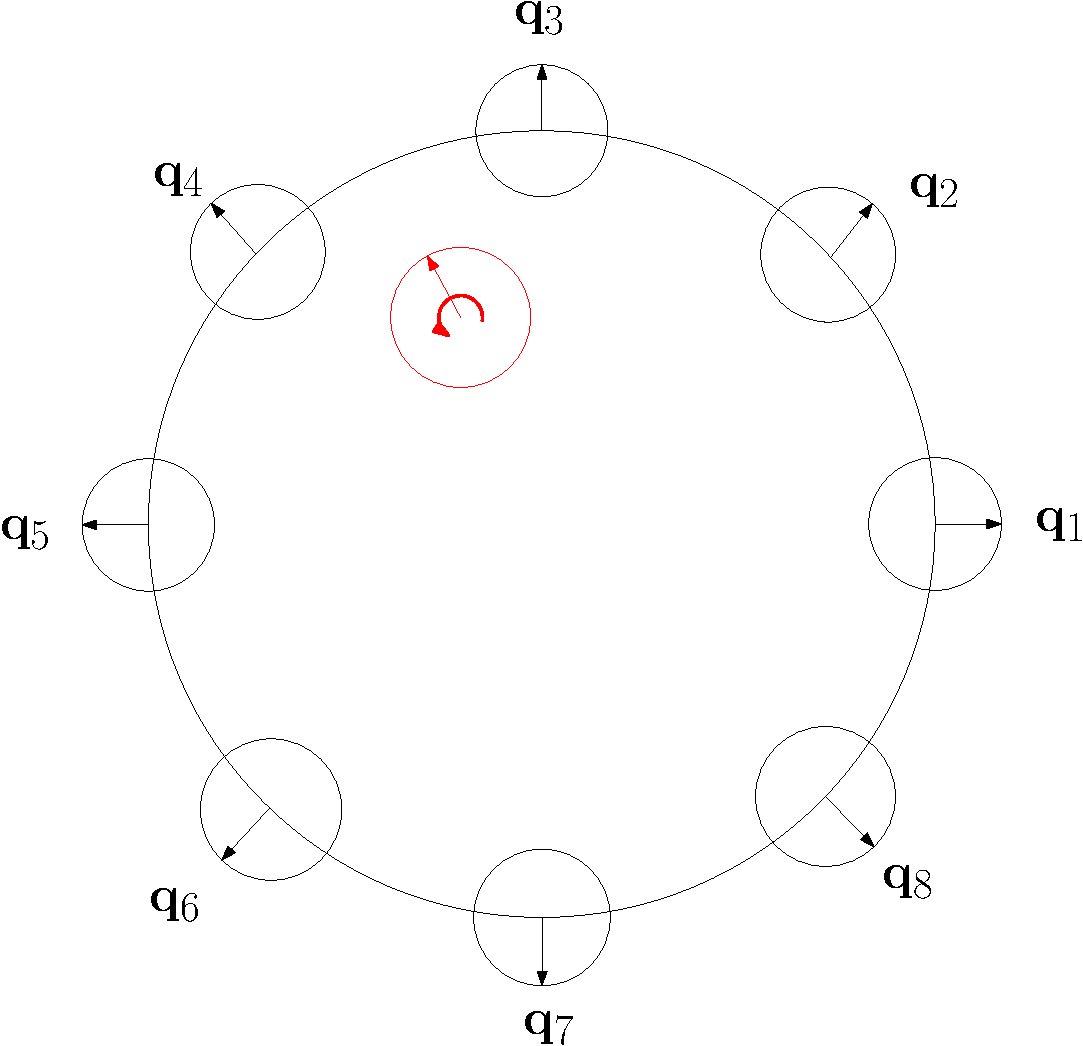
\includegraphics[width=0.48\linewidth]{figs/2/rotation_error.pdf}}
\subfloat[Translational movement]{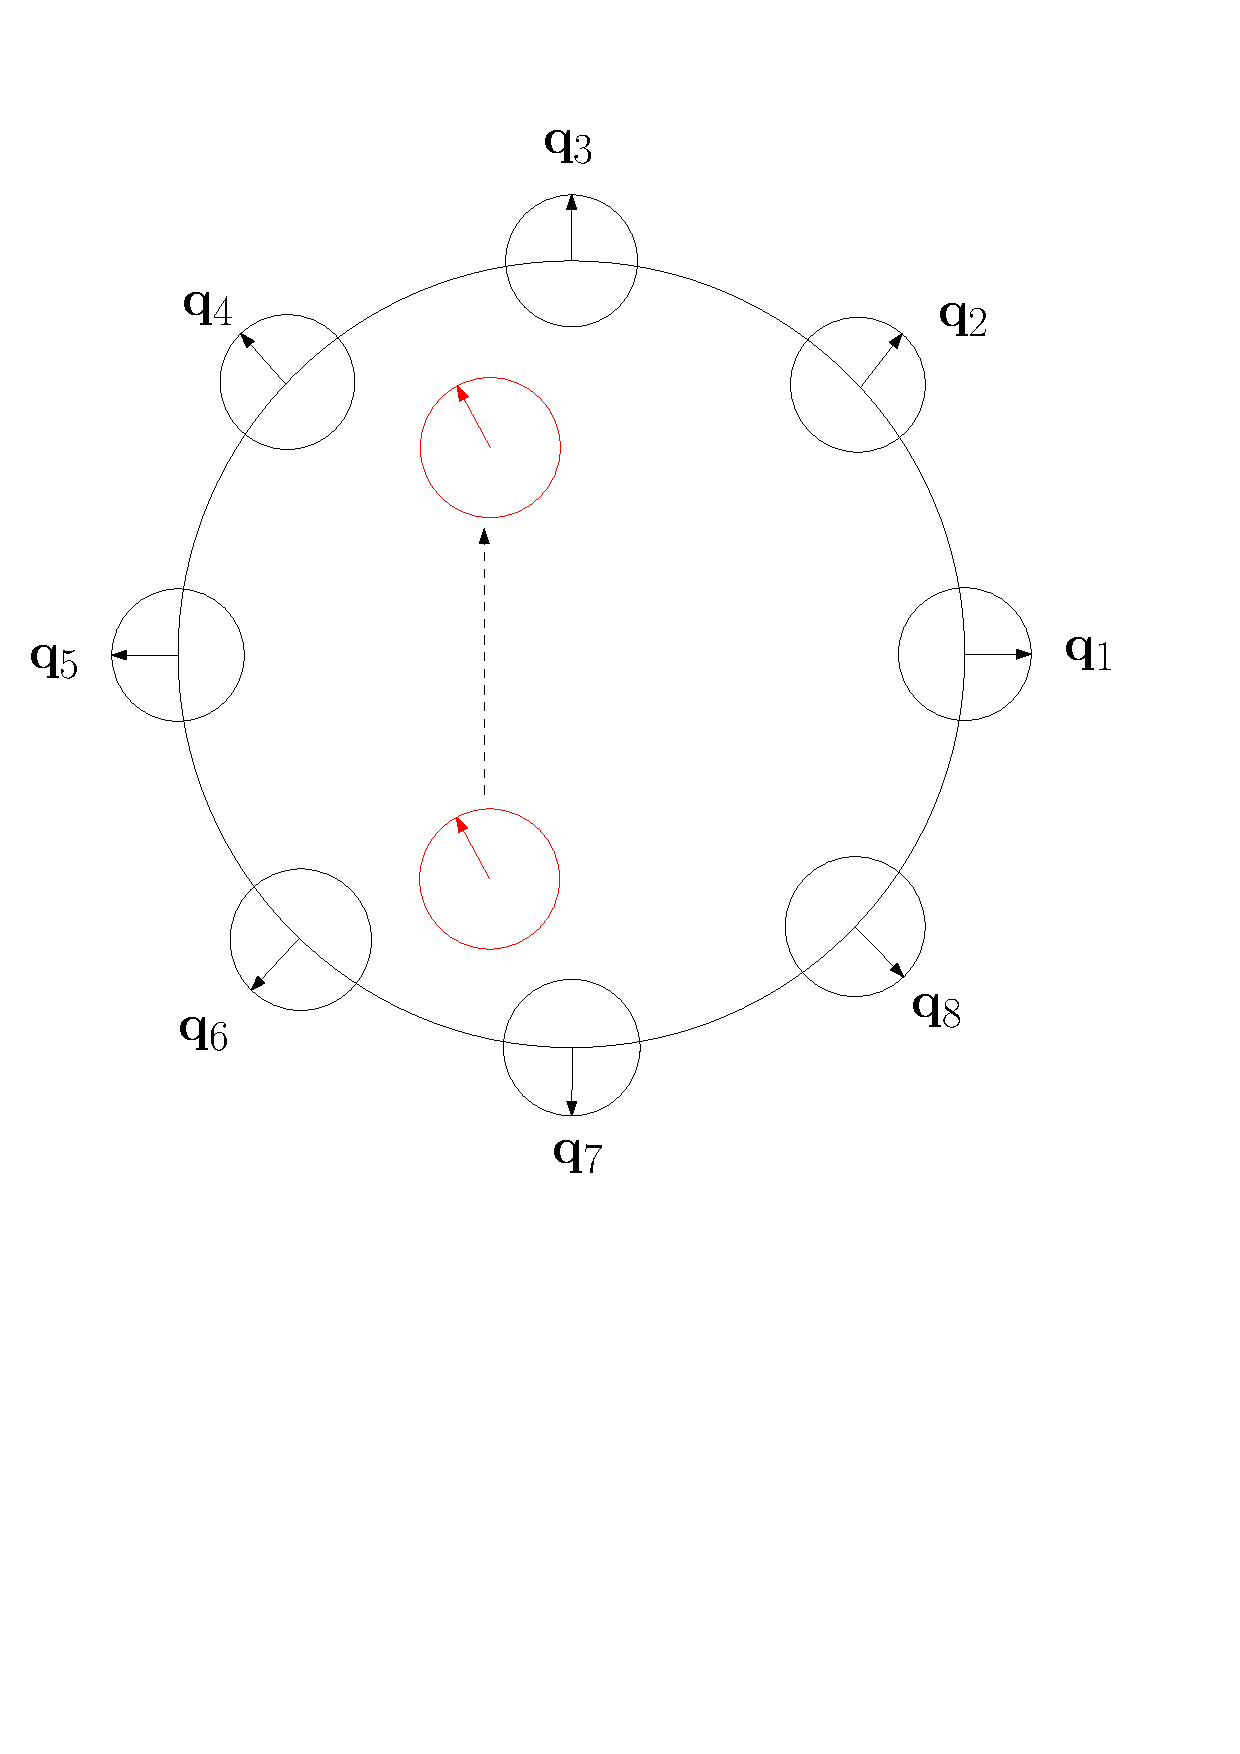
\includegraphics[width=0.48\linewidth]{figs/2/translation_error.pdf}}
\caption[Simple benchmarks for illustrating how the configuration space metric influences the result of our PD algorithm]{Simple benchmarks for illustrating how the configuration space metric influences the result of our PD algorithm. The large sphere is the $\Cobs$. We use small spheres to denote configuration samples in the configuration space: the sphere center is the translational component and the arrow's direction indicates the rotational component. We use eight configurations to approximate the contact space. The red sphere is the query configuration. In (a), the query rotates counter-clockwise. In (b), the query performs translation motion.}\label{fig:2:toybenchmark}
\end{figure}



To better illustrate the above limitation related to configuration space metrics and sampling-based techniques, we now use two simple benchmarks (Figures~\ref{fig:2:toybenchmark}(a) and (b)) to show the behavior of our PD algorithm when different metric settings are used. In these benchmarks, we use eight configuration samples to approximate the contact space. The translational components of these configurations are uniformly distributed on a circle with radius $1$; these configurations have rotation angles of $\frac{k \pi}{4}$, $k=1,...,8$.

\begin{figure}[!h]
\centering
  \subfloat[$\mu_i = 0$]{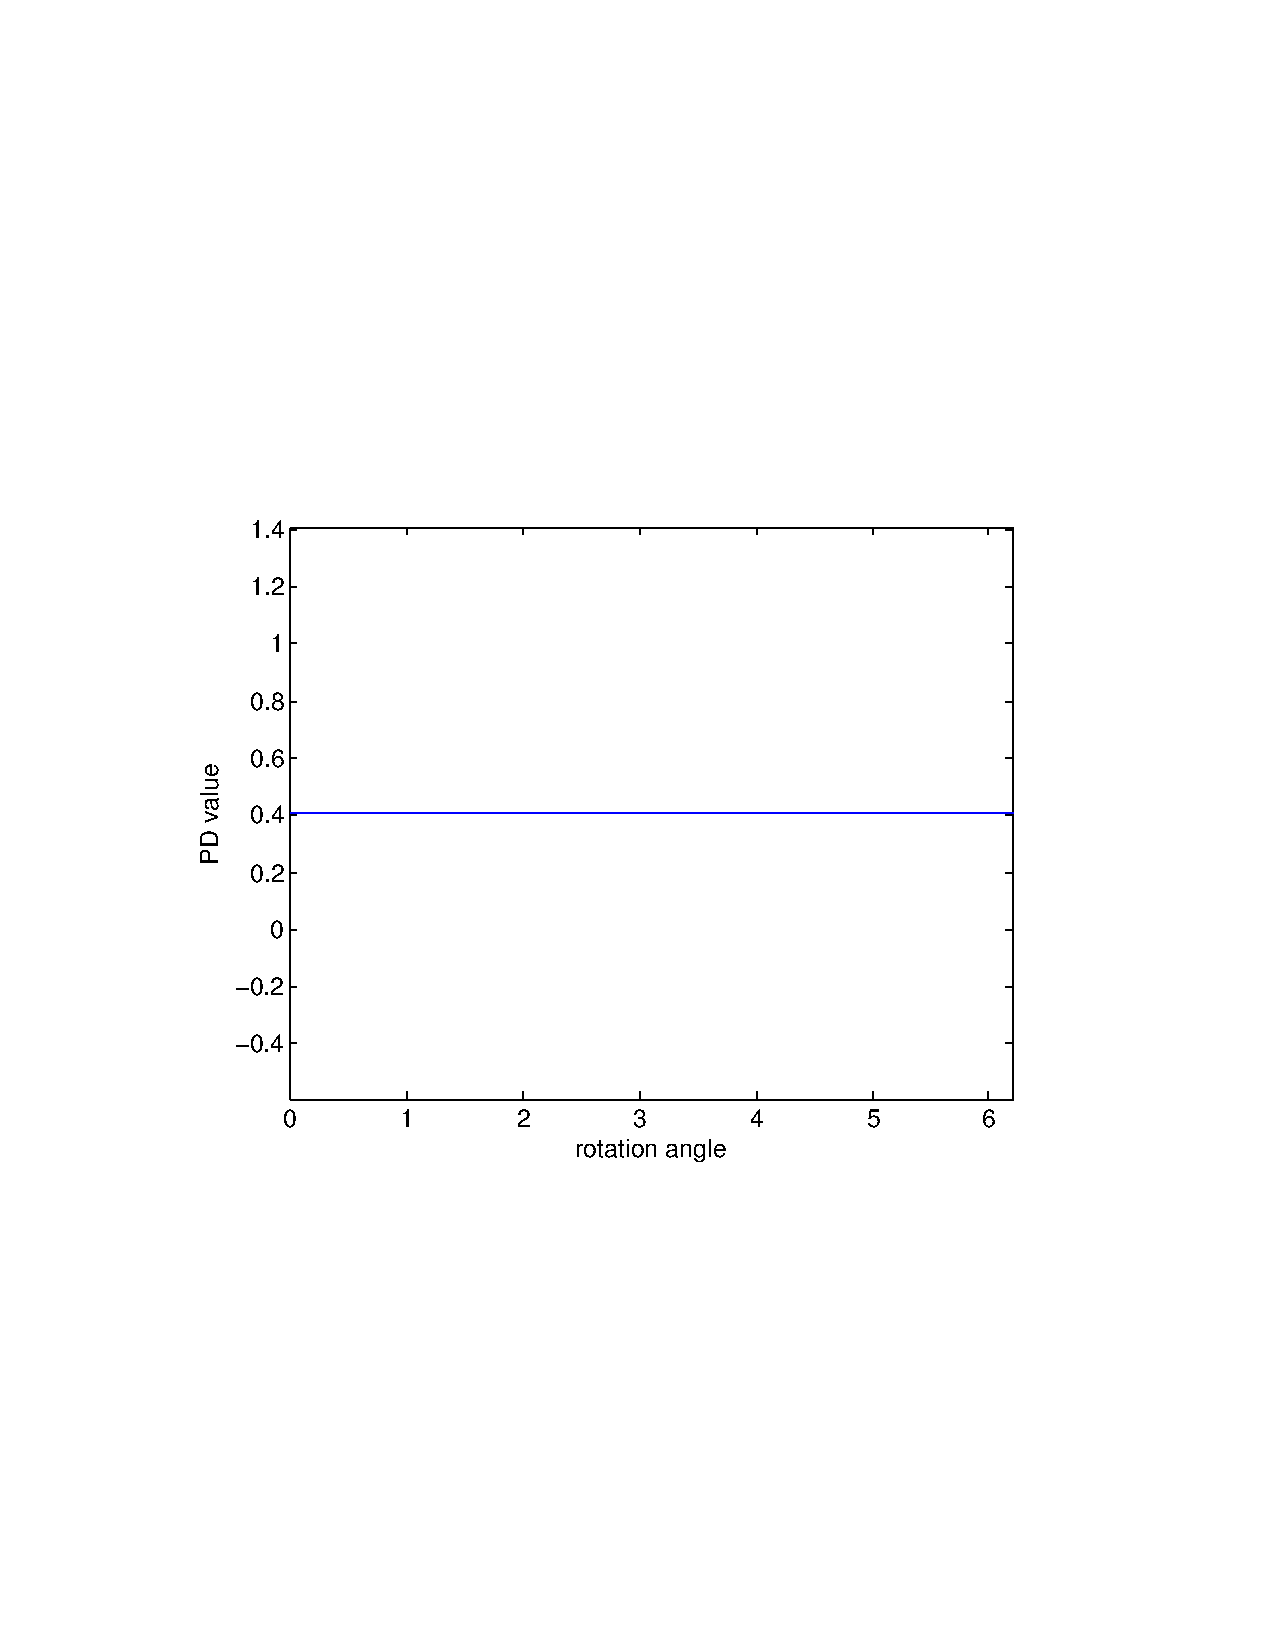
\includegraphics[width=0.33\linewidth, trim=33mm 80mm 40mm 85mm, clip]{figs/2/rotation_error_w00000.pdf}}
  \subfloat[$\mu_i = 0.001$]{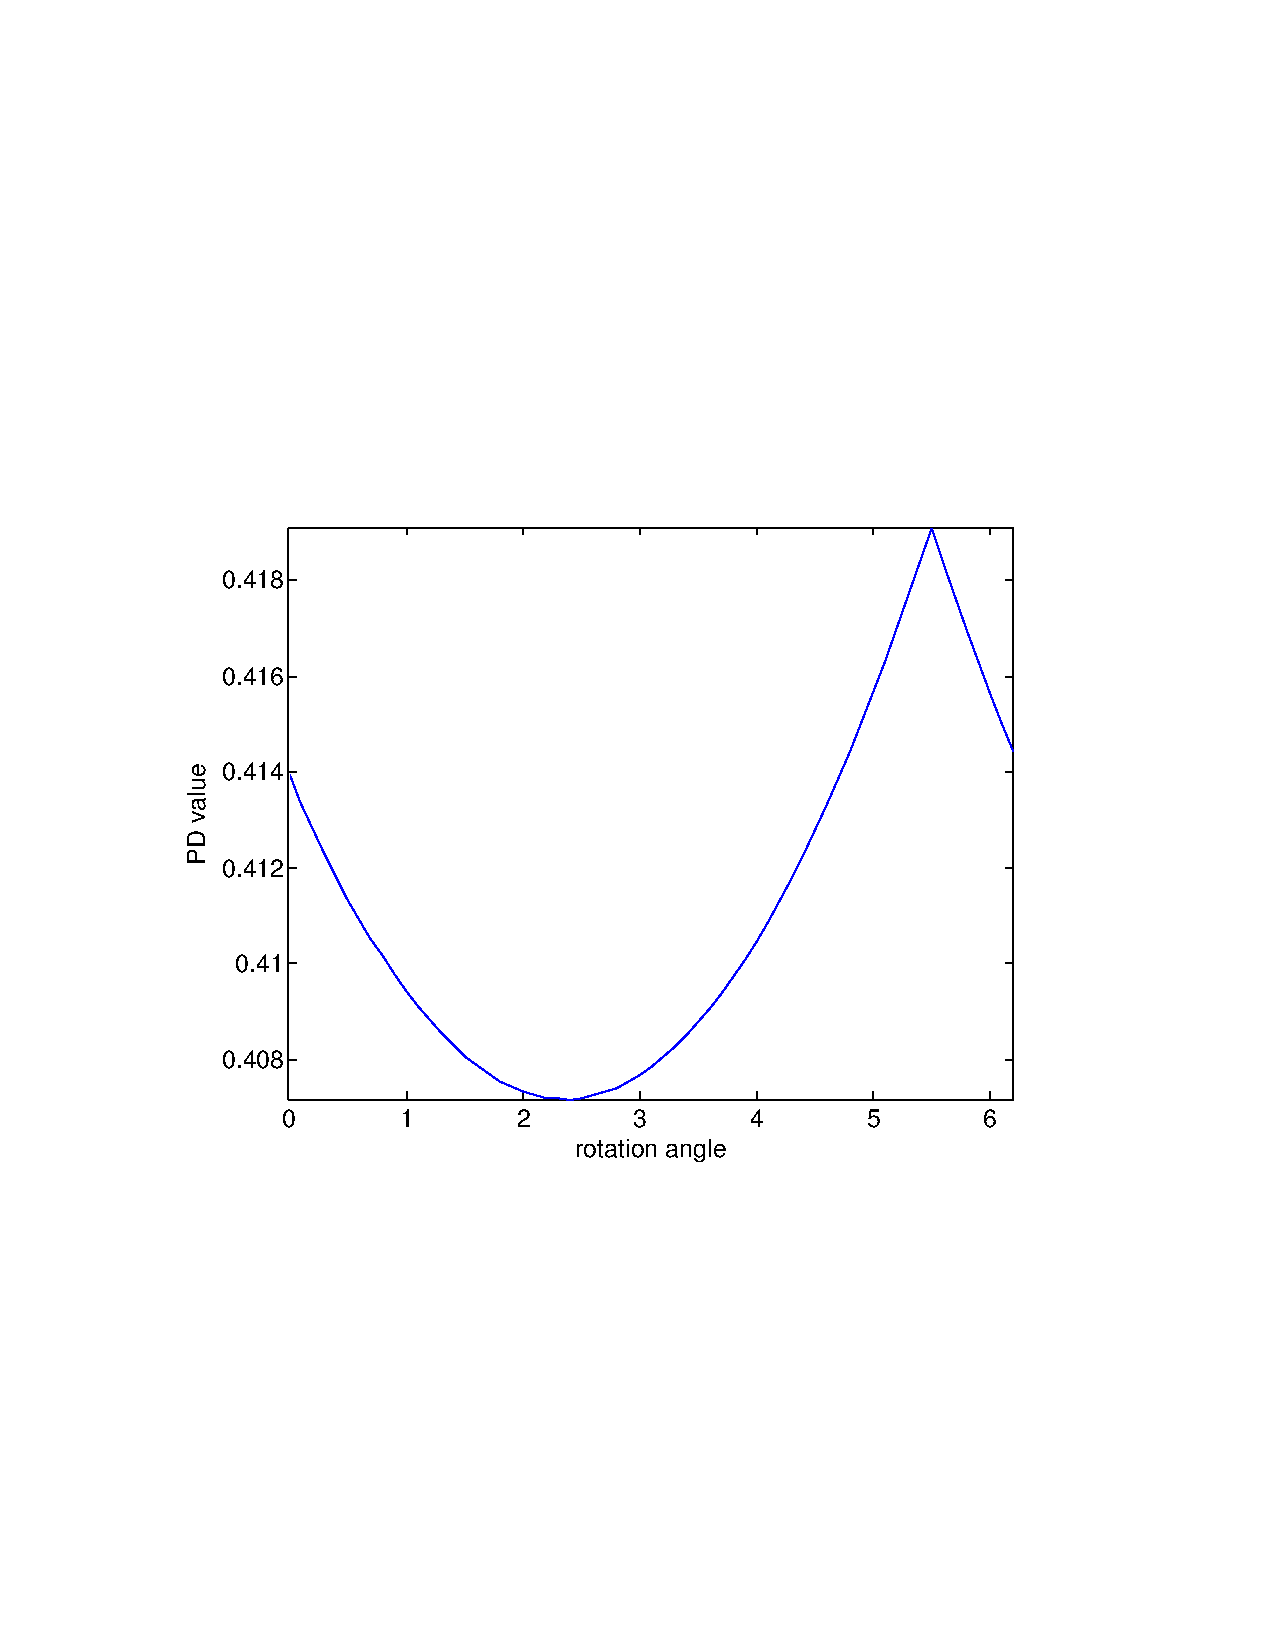
\includegraphics[width=0.33\linewidth, trim=33mm 80mm 40mm 85mm, clip]{figs/2/rotation_error_w0001.pdf}} 
  \subfloat[$\mu_i = 0.01$]{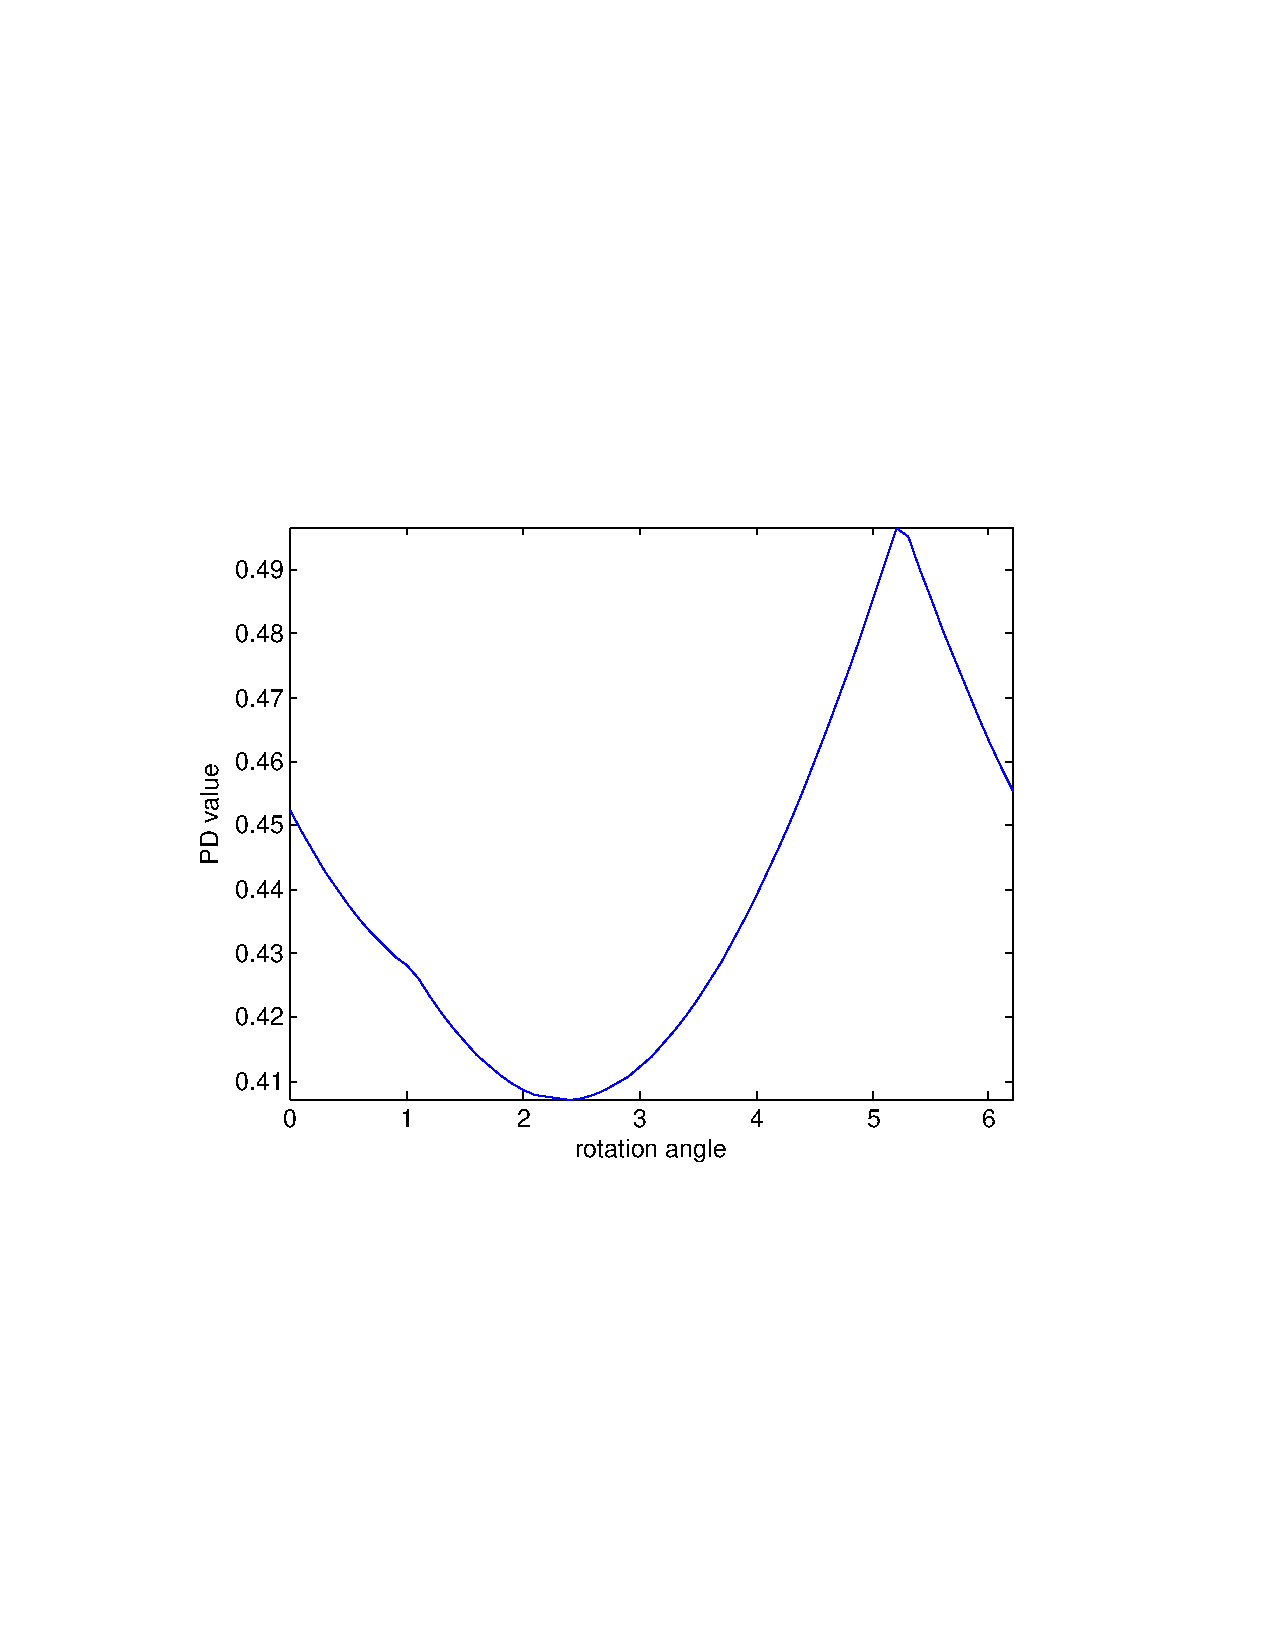
\includegraphics[width=0.33\linewidth, trim=33mm 80mm 40mm 85mm, clip]{figs/2/rotation_error_w001.pdf}} \\
  \subfloat[$\mu_i = 0.1$]{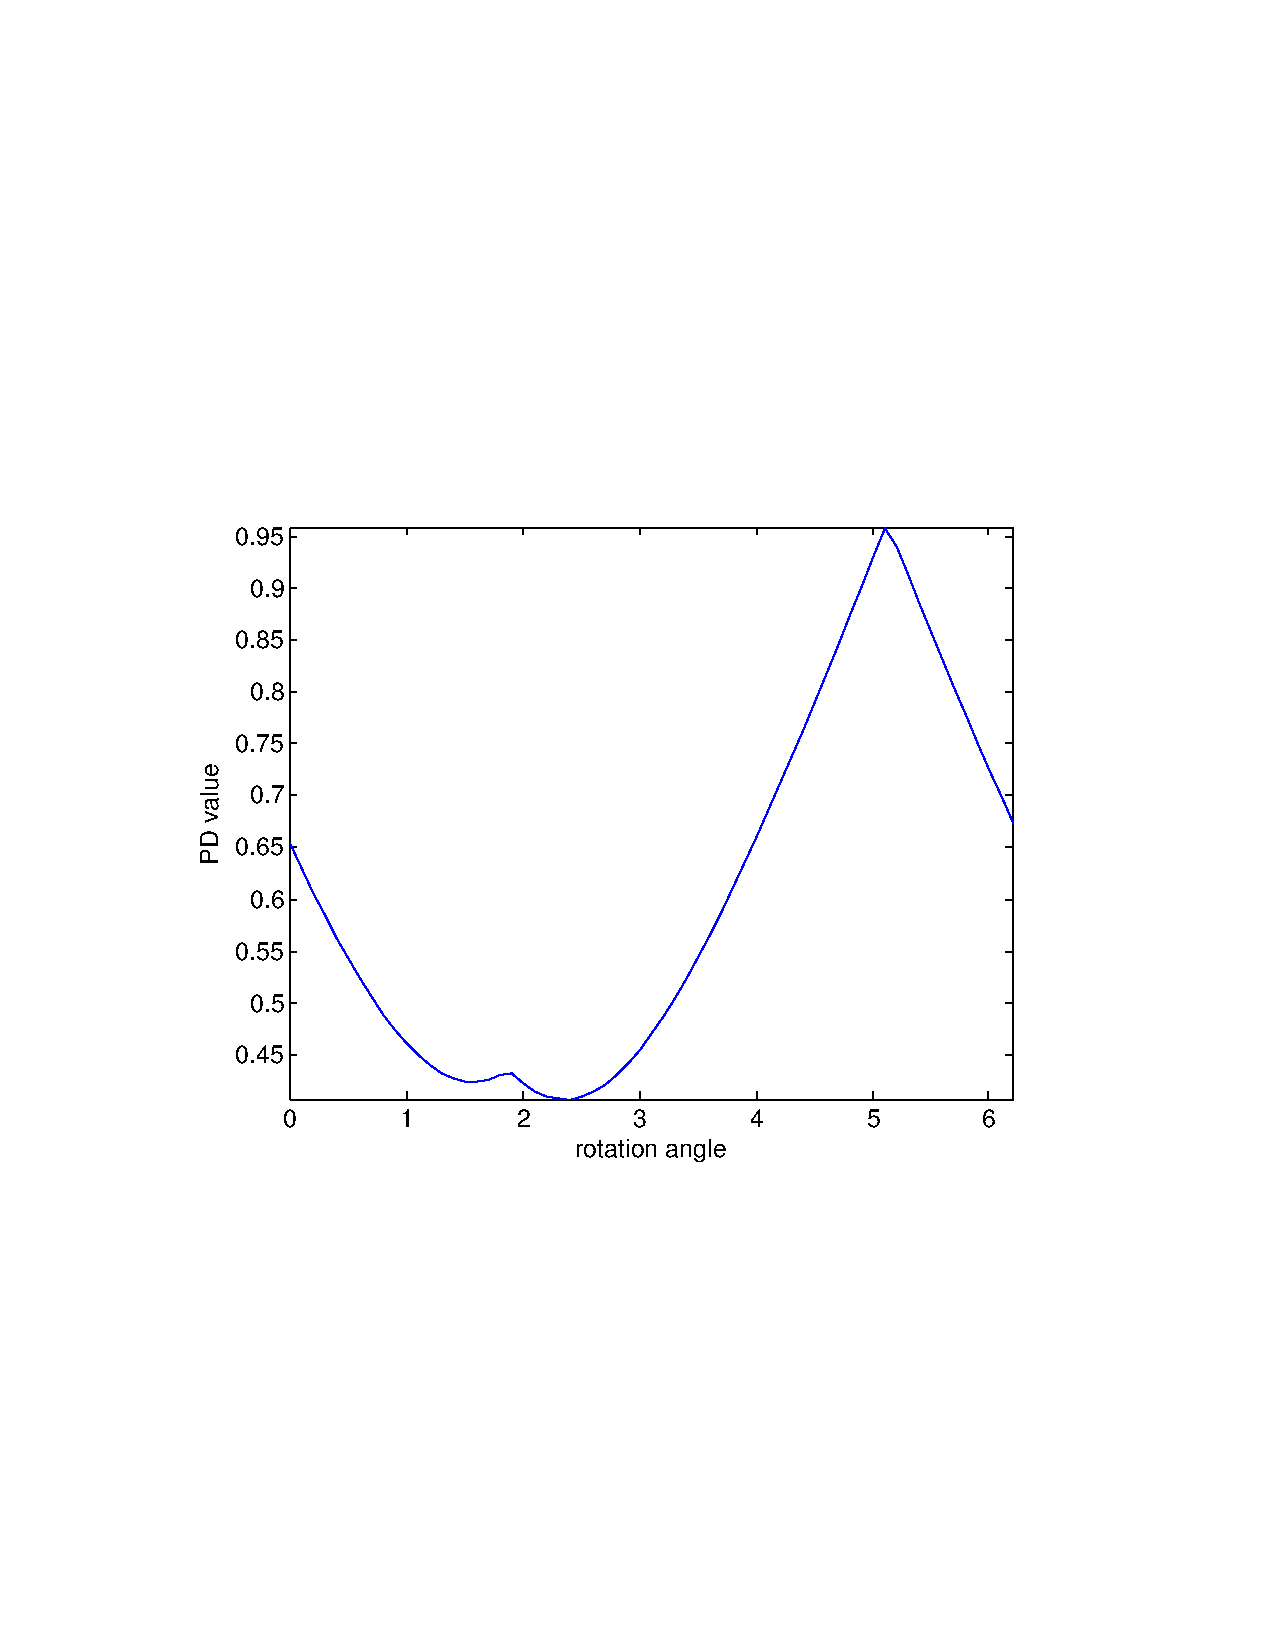
\includegraphics[width=0.33\linewidth, trim=33mm 80mm 40mm 85mm, clip]{figs/2/rotation_error_w01.pdf}}
  \subfloat[$\mu_i = 1$]{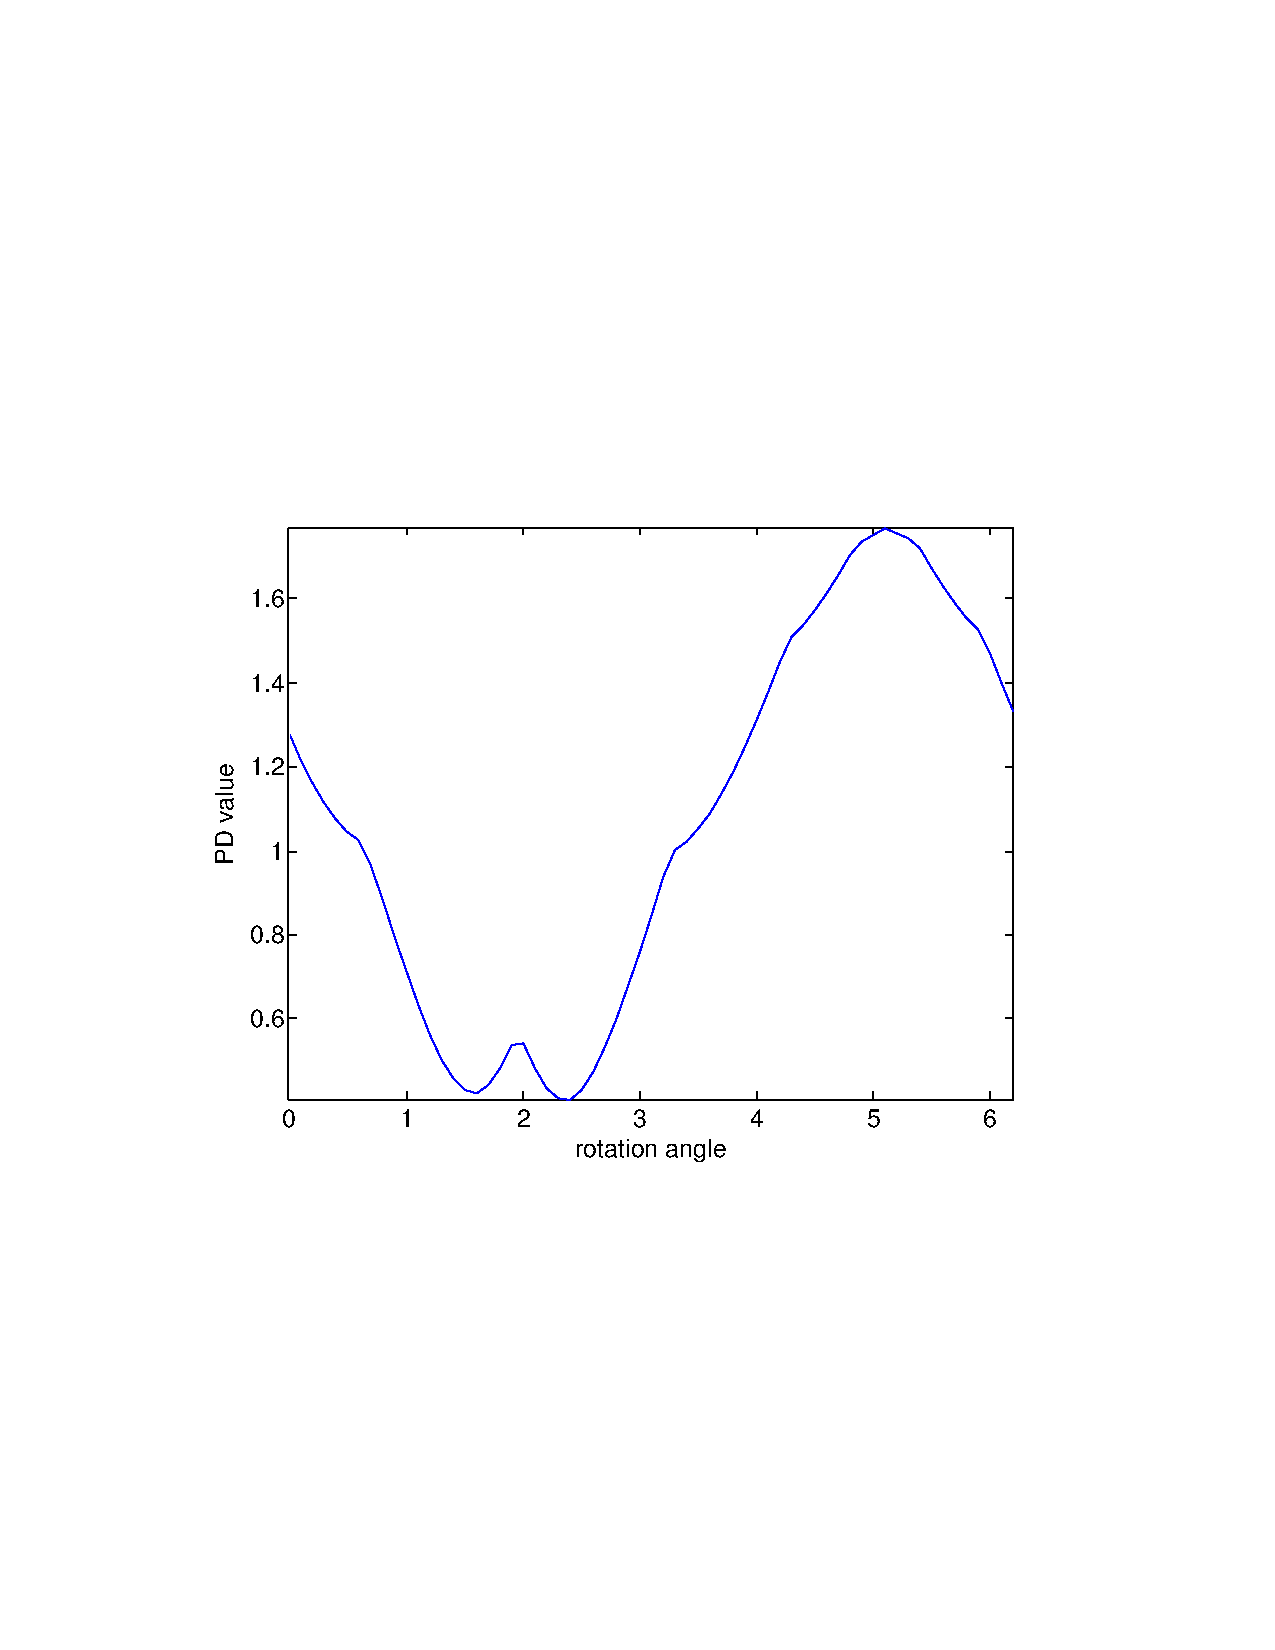
\includegraphics[width=0.33\linewidth, trim=33mm 80mm 40mm 85mm, clip]{figs/2/rotation_error_w1.pdf}}
  \subfloat[$\mu_i = 10$]{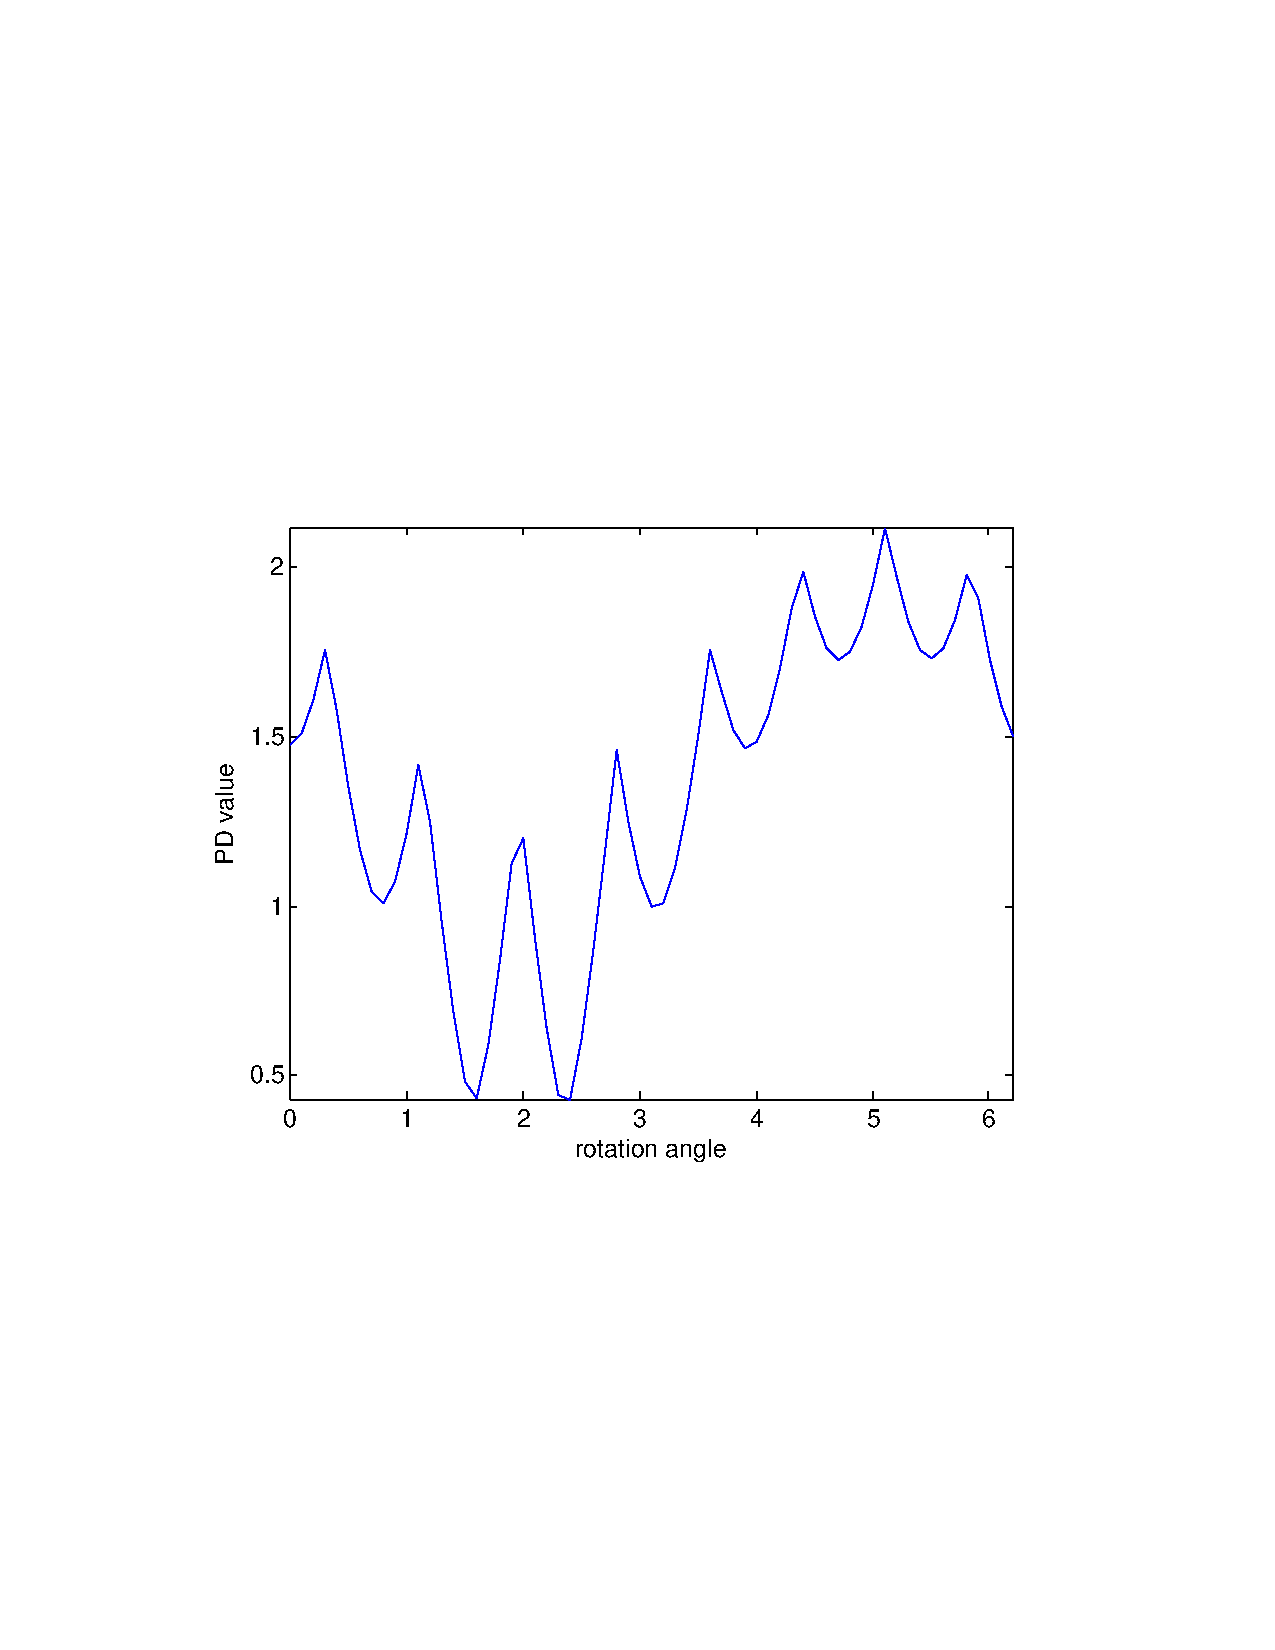
\includegraphics[width=0.33\linewidth, trim=33mm 80mm 40mm 85mm, clip]{figs/2/rotation_error_w10.pdf}} \\
  \subfloat[$\mu_i = 100$]{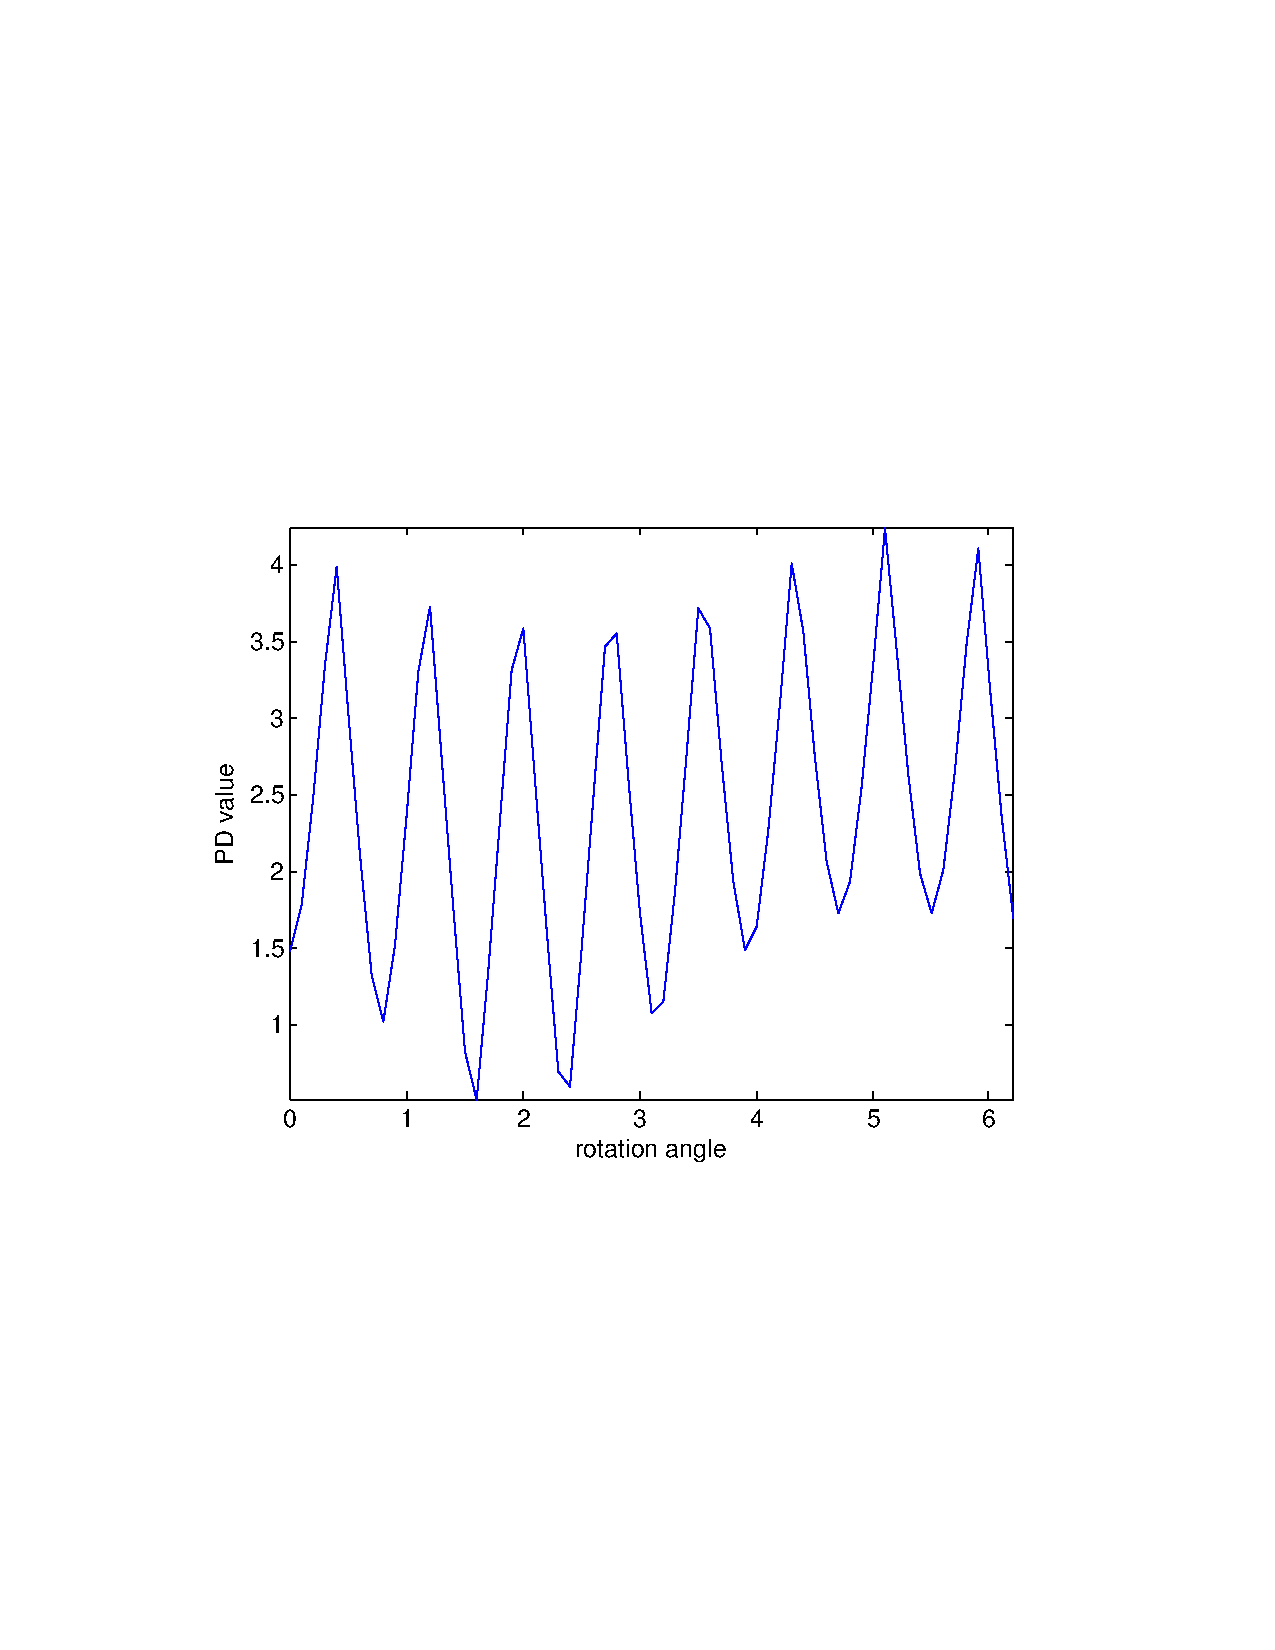
\includegraphics[width=0.33\linewidth, trim=33mm 80mm 40mm 85mm, clip]{figs/2/rotation_error_w100.pdf}}
  \subfloat[$\mu_i = 1,000$]{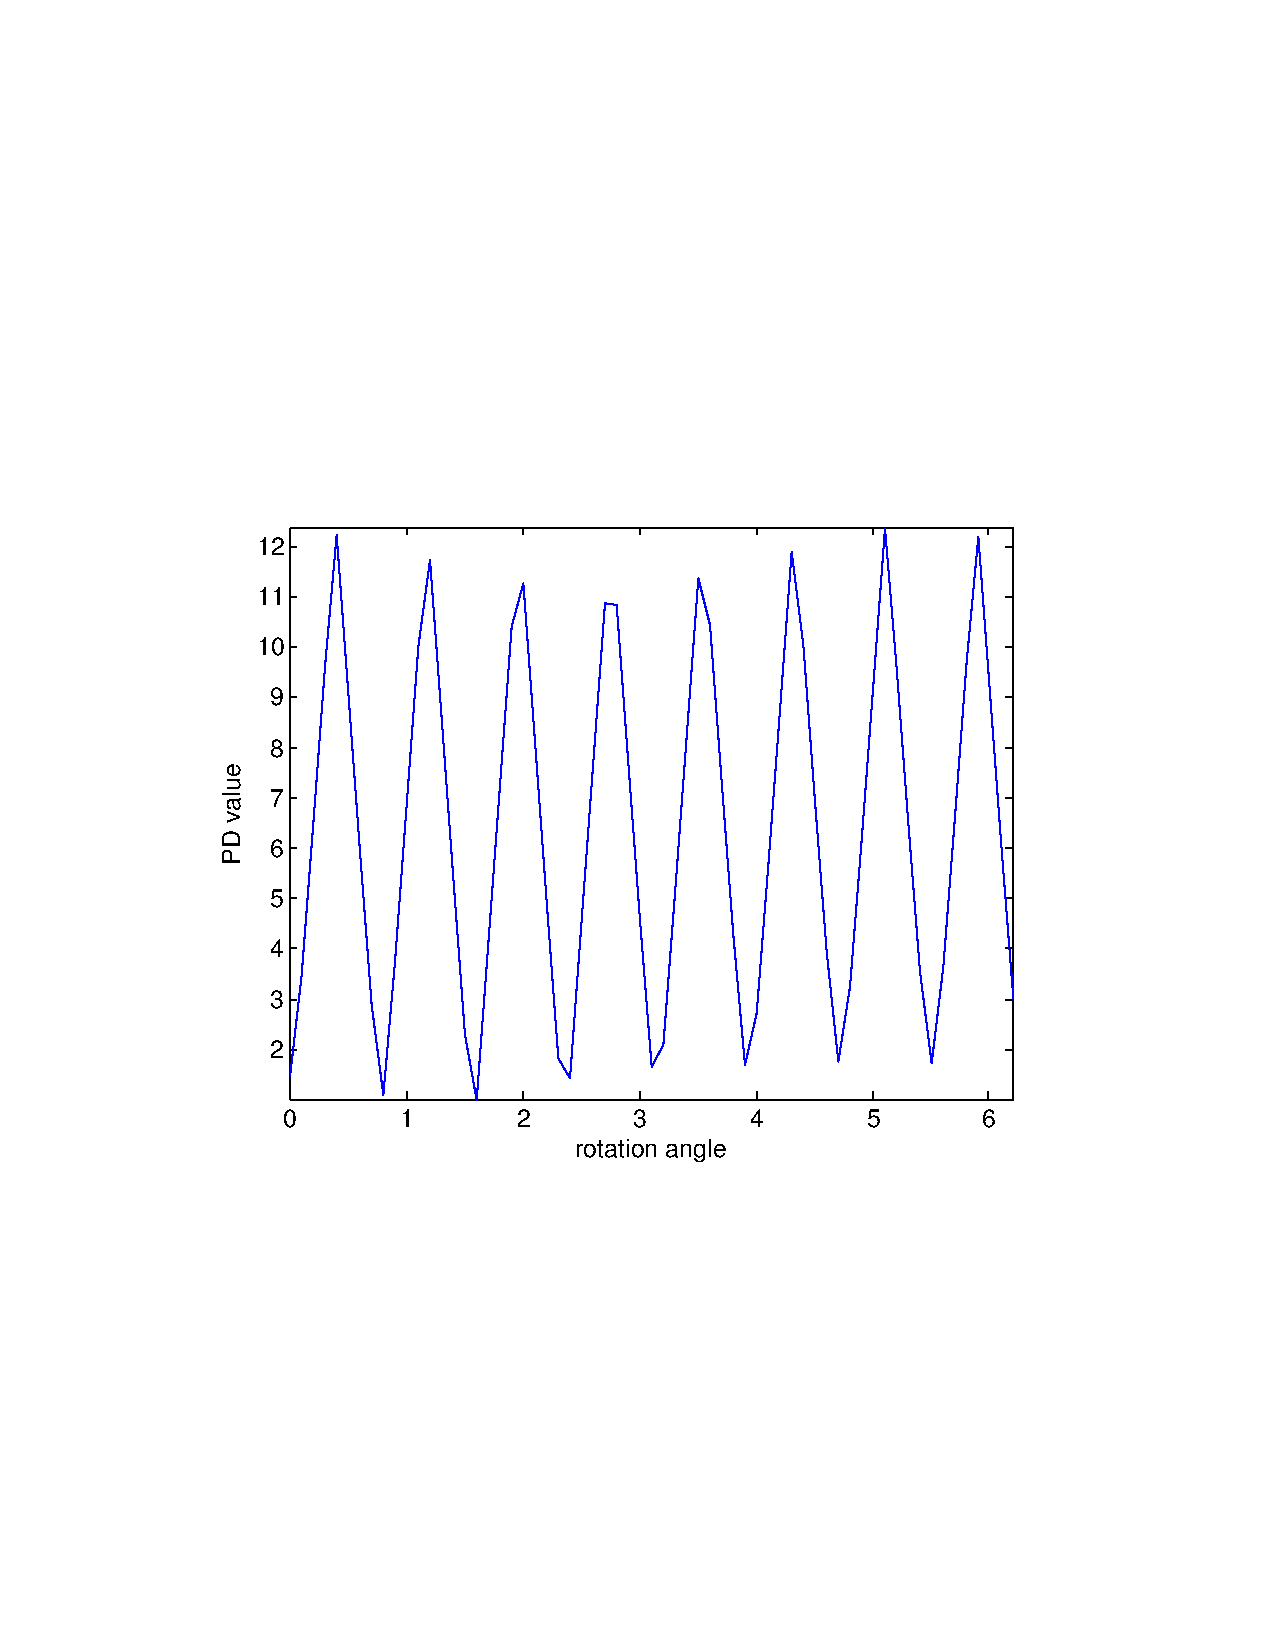
\includegraphics[width=0.33\linewidth, trim=33mm 80mm 40mm 85mm, clip]{figs/2/rotation_error_w1000.pdf}}
  \subfloat[$\mu_i = 10,000$]{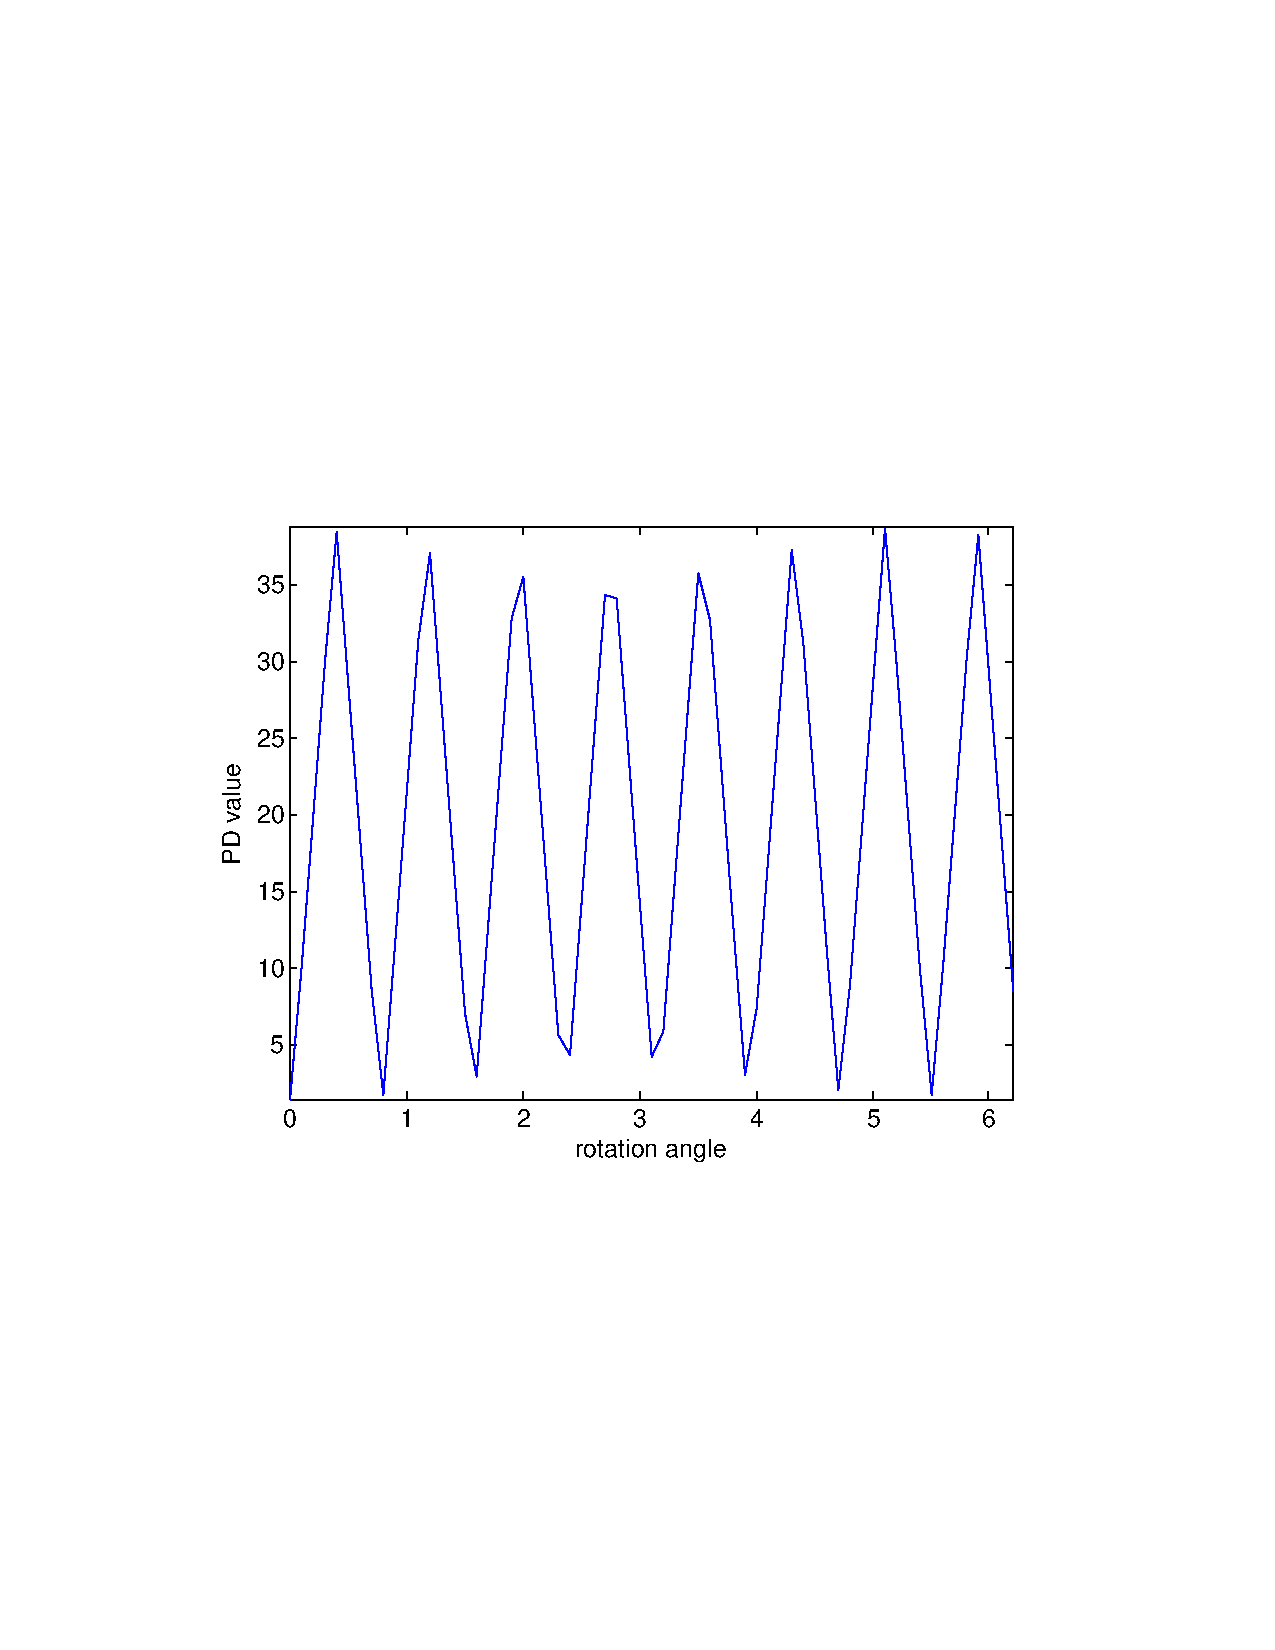
\includegraphics[width=0.33\linewidth, trim=33mm 80mm 40mm 85mm, clip]{figs/2/rotation_error_w10000.pdf}}
\caption[Configuration space metric's influence on the result of our PD algorithm: rotational benchmark]{
The result of our PD algorithm on the rotational benchmark shown in Figure~\ref{fig:2:toybenchmark}(a). We plot the PD values for all query configurations during the rotation, with different $\mu_i$ settings for the configuration space metric.
}\label{fig:2:rotation_error}
\end{figure}


\begin{figure}[!h]
\centering
  \subfloat[$\mu_i = 0$]{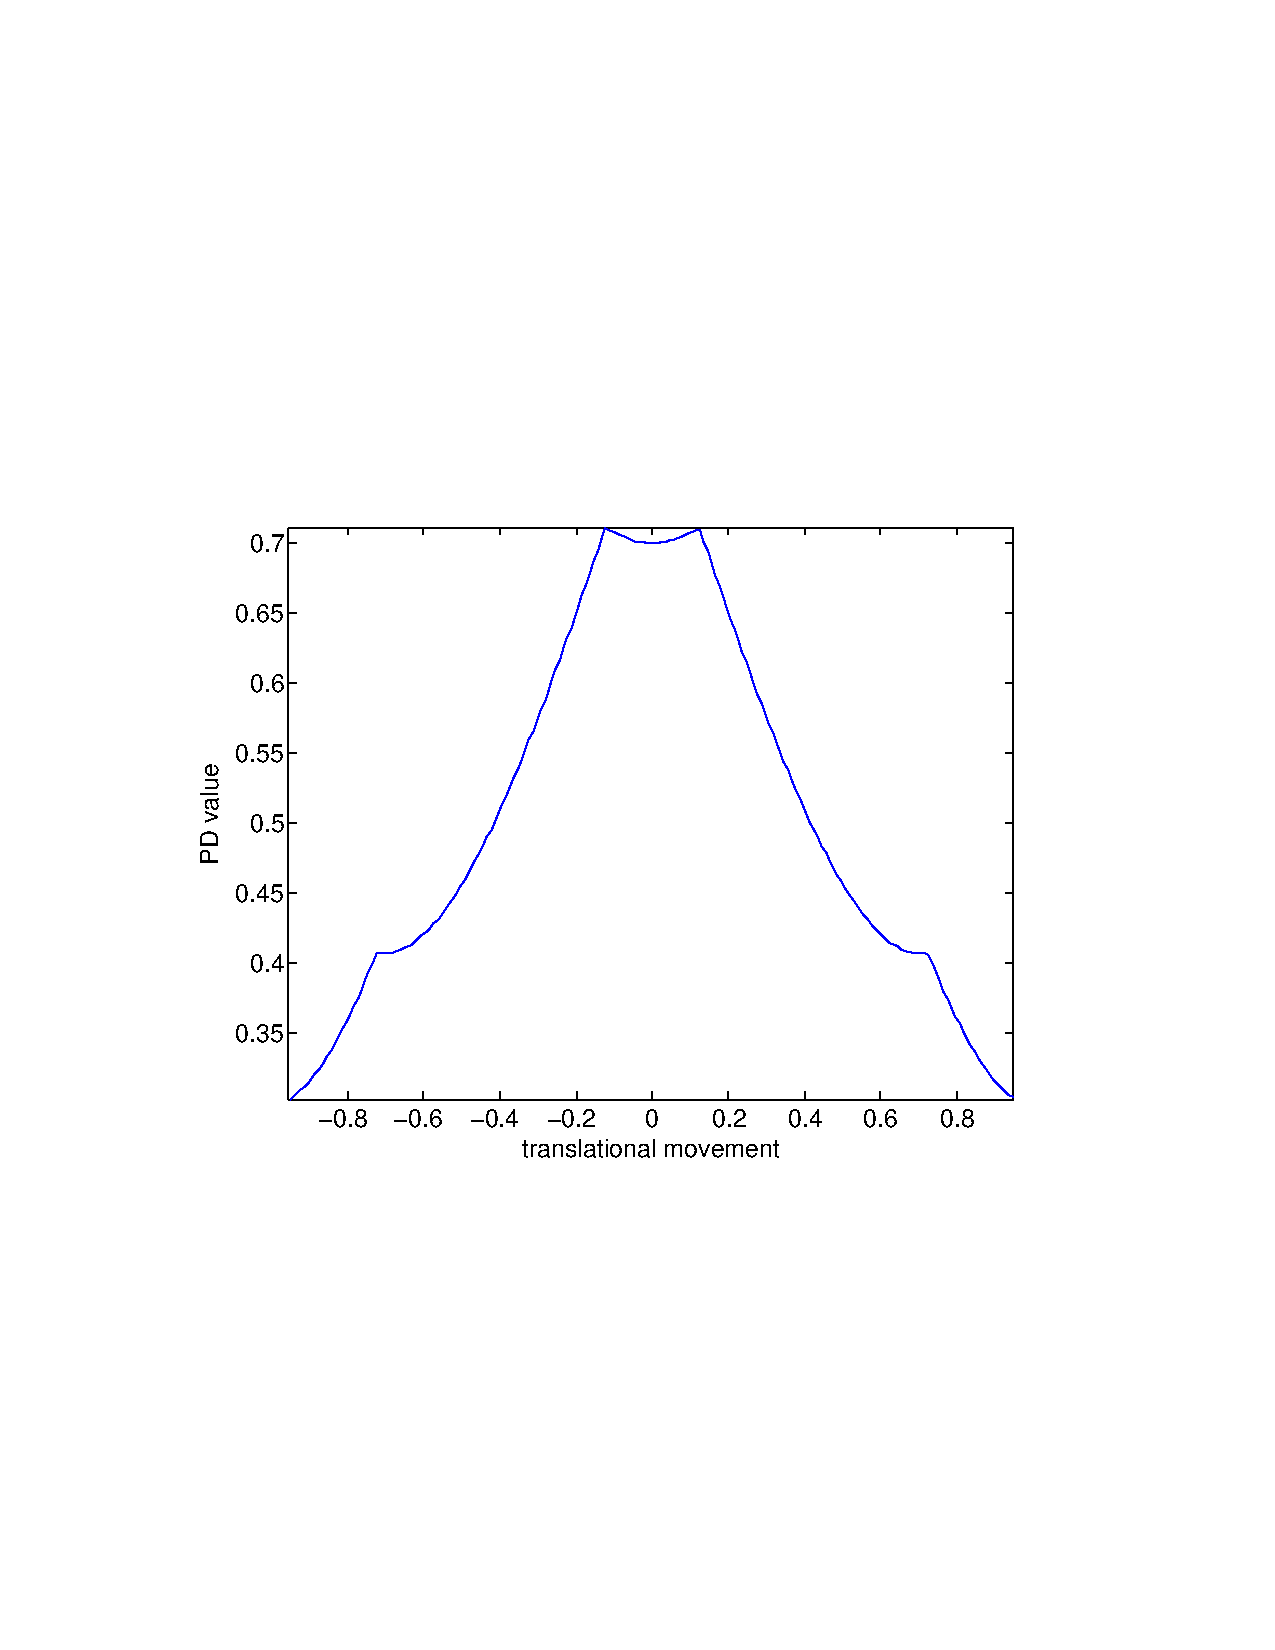
\includegraphics[width=0.33\linewidth, trim=33mm 80mm 40mm 85mm, clip]{figs/2/translation_error_w00000.pdf}}
  \subfloat[$\mu_i = 0.001$]{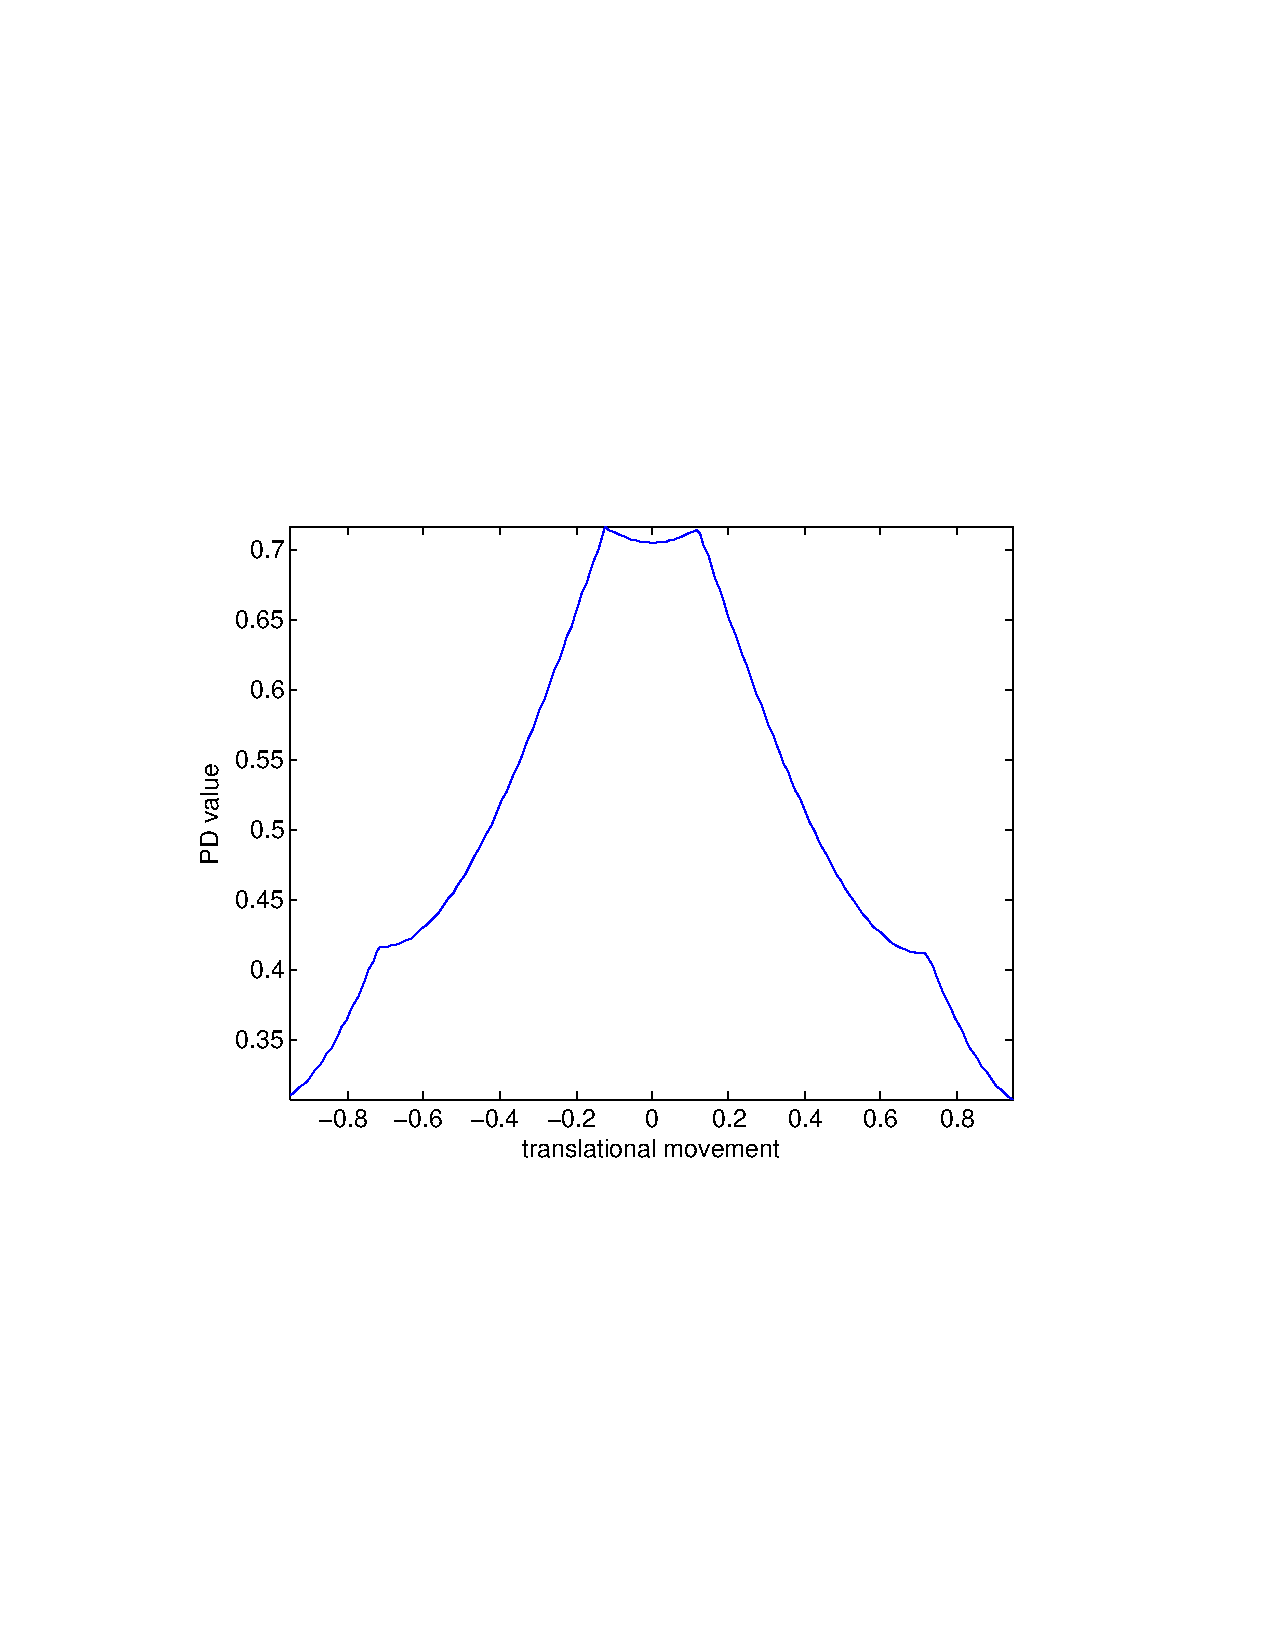
\includegraphics[width=0.33\linewidth, trim=33mm 80mm 40mm 85mm, clip]{figs/2/translation_error_w0001.pdf}} 
  \subfloat[$\mu_i = 0.01$]{\includegraphics[width=0.33\linewidth, trim=33mm 80mm 40mm 85mm, clip]{figs/2/translation_error_w001.pdf}} \\
  \subfloat[$\mu_i = 0.1$]{\includegraphics[width=0.33\linewidth, trim=33mm 80mm 40mm 85mm, clip]{figs/2/translation_error_w01.pdf}}
  \subfloat[$\mu_i = 1$]{\includegraphics[width=0.33\linewidth, trim=33mm 80mm 40mm 85mm, clip]{figs/2/translation_error_w1.pdf}}
  \subfloat[$\mu_i = 10$]{\includegraphics[width=0.33\linewidth, trim=33mm 80mm 40mm 85mm, clip]{figs/2/translation_error_w10.pdf}} \\
  \subfloat[$\mu_i = 100$]{\includegraphics[width=0.33\linewidth, trim=33mm 80mm 40mm 85mm, clip]{figs/2/translation_error_w100.pdf}}
  \subfloat[$\mu_i = 1,000$]{\includegraphics[width=0.33\linewidth, trim=30mm 80mm 40mm 85mm, clip]{figs/2/translation_error_w1000.pdf}}
  \subfloat[$\mu_i = 10,000$]{\includegraphics[width=0.33\linewidth, trim=30mm 80mm 40mm 85mm, clip]{figs/2/translation_error_w10000.pdf}}
\caption[Configuration space metric's influence on the result of our PD algorithm: translational benchmark]{The result of our PD algorithm on the translational benchmark shown in Figure~\ref{fig:2:toybenchmark}(b). We plot the PD values for all query configurations during the translation, with different $\mu_i$ settings for the configuration space metric.}\label{fig:2:translation_error}
\end{figure}


In the first benchmark (Figure~\ref{fig:2:toybenchmark}(a)), the moving object only performs counter-clockwise rotation. The query's rotation angle is $0$ at the beginning and then increases to $2\pi$. If large weights are assigned to the configuration space metric (i.e., $\mu_i$ are large in Equation~\ref{eq:PDgmetricMu}), the query's closest neighbor among the eight contact-space samples would be $\mathbf q_1$, since its rotation angle is also $0$. When the query's rotation angle increases from $0$ to $\pi/4$, the corresponding PD value will first increase and then decrease. This is because the PD value is dominated by the difference in rotation angles: when the rotation angle is close to $0$ or $\pi/4$, this query is either close to $\mathbf q_1$ or to $\mathbf q_2$, and thus the corresponding PD value is small; when the rotation angle is near $\pi/8$, this query is far from both $\mathbf q_1$ and $\mathbf q_2$, and thus the corresponding PD value is large. This phenomenon is shown in Figure~\ref{fig:2:rotation_error}(f)-(i). From these results for large $\mu_i$, we can also observe significant vibrations in PD values when rotation angle changes. The magnitude of such vibrations decreases when parameters $\mu_i$ become smaller (Figures~\ref{fig:2:rotation_error}(a)-(e)). We also observe that the vibration frequency is proportional to the number of samples. In Figure~\ref{fig:2:rotation_error}(a), PD values are constant when $\mu_i = 0$, since rotational weights in the PD metric are zero.

In the second benchmark (Figure~\ref{fig:2:toybenchmark}(b)), the moving object only performs translational motion. In the beginning, the object is in-contact with the obstacles. Then it moves deep inside the obstacles along the $y$-axis. Finally, it will be in-contact with the obstacles again. The query's rotation angle is fixed at $\pi/8$. The results of our PD algorithm are shown in Figure~\ref{fig:2:translation_error}. Apparently, for all $\mu_i$ settings about the metric, PD values are non-zero for in-contact configurations in the beginning and end of the movement. As we discussed above, this is because
we only use a limited number of in-contact configurations to approximate the contact space, and none of them have the same rotation angle as the query. However, if $\mu_i$ is small (Figures~\ref{fig:2:translation_error}(a)-(d)), PD values indeed first increase and then decrease, which is consistent with our intuition; such phenomenon disappears for large $\mu_i$ (Figures~\ref{fig:2:translation_error}(e)-(i)). The reason is that for small $\mu_i$, the translational component dominates the PD value. Since the query's translational distance to the eight in-contact samples first decreases and then increases, the computed PD value will have the same property. For large $\mu_i$, the rotational component dominates the PD value, which does not change because the query's rotation angle is fixed. As a result, the query's PD value only change slightly during the motion, and no longer has the property of first increasing and then decreasing.  Moreover, we observe that for the translational motion, PD values will not have the strong vibration as in the case of the rotational motion, though the PD values are less smooth for smaller $\mu_i$.

Based on above experiments on two benchmarks, we provide a detailed analysis about our PD algorithm's limitation related with configuration space metrics and sampling-based techniques. Our analysis is based on these benchmarks with a few samples in the configuration space. However, the phenomenon we observed about our PD algorithm will also explain our method's behavior when more samples are provided, because for a $6$-dimensional configuration space, even one million samples are still sparse (i.e., $10$ samples for each dimension). Thus, these limitations observed from the toy benchmarks are essential to our learning-based PD framework.

To solve these limitations, a feasible solution is to combine our method with continuous search algorithms such as the optimization-based general PD algorithm~\cite{Tang:IGP:2013}. Given an in-collision query configuration, our method can efficiently compute a candidate for the in-contact configuration $\mathbf q_c$. The optimization-based algorithm can then use $\mathbf q_c$ as an initialization of the optimization and eventually compute an accurate in-contact configuration and the corresponding PD values. Optimization-based algorithm does not use discrete samples to approximate the contact space, and therefore can avoid the ``jump'' and vibration problems of our method.


\section{Conclusions}
We have presented a novel approach for the computation of translational and generalized PD between polygonal models.
The main idea is to sample the configuration space and approximate the contact space based on
machine learning classifiers. We use support vector machines to approximate the contact space, and
the runtime PD query is reduced to nearest neighbor computation. Furthermore,
we use active learning techniques to select the samples when approximating the contact space.
Our overall approach is general and applicable to all polygonal models.
We have demonstrated the interactive performance of our algorithm on complex, non-convex models and have also used
our algorithm for collision response in game physics engines.
To the best of our knowledge, this is the first approach that is able to compute global and reliable PD between rigid models at
interactive rates.


There are many avenues for future work, including overcoming the stated limitations. The basic components of our learning and run-time phases, such as SVM learning, collision detection, and nearest-neighbor computation, can be accelerated using GPU parallelism. We can use other active learning techniques to improve the sampling as well as other classifiers or learning techniques to improve the accuracy or convergence of \LCS. It would also be useful to derive tight theoretical error bounds (e.g., Theorem~1) for active learning algorithms based on exploitation and exploration.
It would also be useful to extend the approach to articulated models that take into account self-collisions between various links.
In order to handle deformable models, we aim to develop incremental techniques that can refine the contact
space approximation for deforming objects. It would be useful to apply this approach for other PD formulations, such as penetration volume~\cite{Weller-RSS-09}, which can result in continuous response forces. We also need improved algorithms for collision response that can guarantee collision-free simulations for interactive applications.

\begin{figure}[!h]
\centering
\parbox{0.9\linewidth}{%
 \subfloat[]{\includegraphics[height=0.605\linewidth]{figs/2/demo/Box2D/Box2DAngryBird_2013_5_14.png}}
 \subfloat[]{\includegraphics[height=0.605\linewidth]{figs/2/demo/Bullet/BulletRainfall.png}}
}
\parbox{0.85\linewidth}{%
  \subfloat[]{\includegraphics[width=0.325\linewidth]{figs/2/demo/star_spoon.png}}
  \subfloat[]{\includegraphics[width=0.325\linewidth]{figs/2/demo/cup_spoon.png}}
  \subfloat[]{\includegraphics[width=0.325\linewidth]{figs/2/demo/teeth.png}}\\
  \subfloat[]{\includegraphics[width=0.325\linewidth]{figs/2/demo/bunny_bunny.png}}
  \subfloat[]{\includegraphics[width=0.325\linewidth]{figs/2/demo/dragon_dragon.png}}
  \subfloat[]{\includegraphics[width=0.325\linewidth]{figs/2/demo/buddha_buddha20K.png}}
}
\caption[Learning-based PD computation algorithm computes a global penetration depth between overlapping non-convex and non-manifold objects]{Our algorithm computes a global penetration depth between overlapping non-convex and non-manifold objects. (a) Dynamic simulation of angry bird characters falling into a complex chute in the Box2D physics engine; (b) rainfall of $1,000$ rings in the Bullet physics engine; (c) a star and a spoon; (d) a spoon and a cup; (e) multiple contacts between upper and lower teeth (each has more than $40,000$ triangles). (f-h) benchmarks consisting of complex models (bunny, dragon and Buddha models have $70K$, $230K$ and $1M$ triangles, respectively). For each pair of overlapping objects, our PD algorithm takes less than $0.1\sim2$ milliseconds, with less than 2-3\% relative error.}\label{fig:2:demo}
\end{figure}


\begin{table}[!h]
  \centering
  \rowcolors{1}{gray!25}{}
  \resizebox{\linewidth}{!}{%
    \begin{tabular}{|c|r|r|r|r|r|r|r|r|r|r|r|r|r|r|}
    \hline
    \multicolumn{2}{|c|}{\multirow{3}{*}{Model}} & \multicolumn{8}{c|}{Offline Learning  \LCS} & \multicolumn{5}{c|}{Runtime Query}\\
    \cline{3-15}
    \multicolumn{2}{|c|}{} & \multicolumn{2}{c|}{Initial Learning} & \multicolumn{4}{c|}{Active Learning} & \multicolumn{1}{c|}{\multirow{2}{*}{total (s)}} & \multicolumn{1}{c|}{\multirow{2}{*}{mem}} & \multicolumn{4}{c|}{time (ms)} & \multicolumn{1}{c|}{\multirow{2}{*}{$e_{\text{PD}}$(\%)}}\\
    \cline{3-8} \cline{3-8} \cline{11-14}
    \multicolumn{2}{|c|}{} & \#smpls & time (s) & \#smpls & $|S|$ & $e_{\text{col}}$ (\%) & time (s) & \multicolumn{1}{c|}{}& \multicolumn{1}{c|}{}&  NN & projection & refine & total & \multicolumn{1}{c|}{}\\
    \hline \hline
    \multicolumn{1}{|c|}{\multirow{3}{*}{2D $\PDt$}} & star vs. room & 100   & 0.006 & 1000 & 374   & 1.88 & 0.15  & 0.156 &  4.4  & 0.065 & 0.02 & 0.03 & 0.115 & 0.023\\
    \multicolumn{1}{|c|}{} & monkeys & 100   & 0.4   & 1000 & 346   & 0.11 & 2.74  & 3.14 &  4.2  & 0.06 & 0.01 & 0.03   & 0.10 & 0.008 \\
    \multicolumn{1}{|c|}{} & spiders & 100   & 0.01  & 1000 & 389   & 1.37 & 0.27  & 0.28 &  4.7  & 0.066 & 0.01 &  0.02  & 0.096 & 0.025 \\ \hline
    \multicolumn{1}{|c|}{\multirow{3}{*}{3D $\PDt$}} & star vs. spoon & 1000  & 0.08  & 10000 & 1105  & 0.59 & 1.245 &  1.33 &  17  & 0.43 & 0.21 & 0.02  & 0.66 & 0.012\\
    \multicolumn{1}{|c|}{} & cup vs. spoon & 1000  & 0.25  & 10000 & 1472  & 0.75 & 4.46 & 4.81 &   23  & 0.54 & 0.22 &  0.03  & 0.79 & 0.019 \\
    \multicolumn{1}{|c|}{} & rings & 1000  &  0.20 & 10000 & 1224  & 0.56 & 11.99 & 12.01 & 19    & 0.66 & 0.12 &  0.05   &  0.83 & 0.016 \\
    \multicolumn{1}{|c|}{} & teeth  & 1000  &  0.33 & 10000 & 2132  & 1.3 & 43.21 & 43.54 &  34   & 1.3 & 0.2 &  0.08  &  1.58 & N/A \\
    \multicolumn{1}{|c|}{} & bunnies  & 1000  &  0.15 & 10000 & 666  & 1.7 & 36.49 & 36.64 &   11    & 0.1 & 0.12 &  0.04  & 0.26 & 2.0 \\
    \multicolumn{1}{|c|}{} & dragons  & 1000  &  0.17 & 10000 & 854  & 1.8 & 31.11 & 31.28 &   14    & 0.13 & 0.11 &  0.05  &  0.29 & 1.9 \\
    \multicolumn{1}{|c|}{} & Buddha  & 1000  &  1.7 & 10000 & 1384  & 1.8 & 37 & 38 &   22    & 0.18 & 0.10 &  0.09  &  0.37 & 1.8 \\
    \hline \hline
    \multicolumn{1}{|c|}{\multirow{3}{*}{2D $\PDg$}} & star vs. room &  100   & 0.005 & 2000 & 436  & 2.0 & 1.276 & 1.281 &  6.9   & 0.08 & 0.03 &  0.02    & 0.13 & 0.021\\
    \multicolumn{1}{|c|}{} & monkeys & 100 & 0.42   &  2000 & 545   & 0.43 &  5.84 &  6.26 &    8.7    & 0.07 & 0.02  & 0.02  & 0.11 & 0.013 \\
    \multicolumn{1}{|c|}{} & spiders & 100 & 0.011 & 2000   & 540  &  0.8 &  1.16 & 1.17 &   8.6   & 0.08 & 0.02 &   0.01   & 0.11 & 0.018 \\ \hline
    \multicolumn{1}{|c|}{\multirow{3}{*}{3D $\PDg$}} & star vs. spoon &  1000 & 0.095  & 10000  & 1731  & 1.9 & 37.49 & 37.58 &  48   &0.5 & 0.25 &  0.05  & 0.80 & N/A \\
    \multicolumn{1}{|c|}{} & cup vs. spoon & 1000 & 0.3  & 10000   &  2107  & 1.2  &  78.34 & 78.64 &  59   & 0.3& 1.0 & 0.03  &  1.33 & N/A \\
    \multicolumn{1}{|c|}{} & rings & 1000  & 0.25  & 10000   &  1977  &  1.3  &  223.1 & 223.4 &   55    & 0.82 & 0.21 &   0.03  & 1.06 & N/A \\
    \multicolumn{1}{|c|}{} & teeth  & 1000  &  0.54 & 10000 & 3216  & 2.8 & 476.43 & 476.97 &   90      & 2.2 & 0.2 & 0.04  &  2.44 & N/A \\
    \multicolumn{1}{|c|}{} & bunnies  & 1000  &  0.33 & 10000 & 2283  & 3.1 & 342.31 & 342.64 &   64     & 0.89 & 0.12 & 0.02  &  1.03 & N/A \\
    \multicolumn{1}{|c|}{} & dragons  & 1000  &  0.37 & 10000 & 2387  & 2.8 & 378.92 & 477.29 &   69     & 1.01 & 0.18 & 0.03  &  1.22 & N/A \\
    \multicolumn{1}{|c|}{} & Buddha  & 1000  &  2.3 & 10000 & 3765  & 2.7 & 643 & 645 &   105     & 1.20 & 0.28 & 0.07  &  1.55 & N/A \\
    \hline
    \end{tabular}
}
  \caption[Performance of the learning-based PD algorithm on 2D and 3D models]{
Performance of our PD algorithm on 2D and 3D models: The learning phase includes the number of samples, size of support vectors, final memory usage (KB), and precomputation time.
We also give a timing breakdown of runtime queries. The PD error is computed by comparing the accuracy of $\overline{\text{PD}}$ with prior algorithms used for PD computations. For accurate $\PDt$ computation, we use the accurate, offline algorithm of~\protect \cite{Lien:2009:ASM} or use a combination of convex decomposition and Minkowski sums.   Since no accurate and efficient algorithms are known for many PD queries (e.g., $\PDt$ computation for non-closed meshes like teeth model; $\PDg$ computation for 3D models), we do not analyze the accuracy of our algorithm in such cases (shown as N/A). }\label{tab:2:learningperformance}
\end{table}














\chapter[Configuration Space Approximation using Instance-based Learning]{Configuration Space Approximation \mbox{using} \\ Instance-based Learning} 
\label{chp:IBL}

\section{Introduction}
In motion planning algorithms such as~\cite{Kavraki96, Kuffner00}, the collision detection module is widely used as an oracle to collect information about the free space and approximate its topology. This module classifies a given configuration or a local path as either collision-free (i.e., in $\Cfree$) or in-collision (i.e., overlaps with $\Cobs$). Most motion planning algorithms tend to store only the collision-free samples and local paths, and use them to compute a global path from the initial configuration to the goal configuration. Typically, the in-collision configurations or local paths are discarded.

In this chapter, we incrementally construct an approximate $\Cspace$ representation by exploiting all prior or historical information related to collision queries. The approximate $\Cspace$ representation will improve the performance of the sample-based planner. In previous work, some planners utilized the in-collision configurations or the samples near the boundary of the configuration obstacles (i.e., $\Ccont$) to bias the sample generation or improve the performance of planners in narrow passages~\cite{Boor:1999:ICRA,Jory:2011:IROS,Rodriguez:2006,Zheng:2005}. However, it can be expensive to perform geometric reasoning based on the outcome of a large number of collision queries in high-dimensional spaces. As a result, most prior planners only use partial or local information about configuration spaces, and cannot provide any guarantees in terms of improving overall performance over time.
\subsection{Main Results}
We present a novel approach which improves the performance of sample-based planners by learning from prior instances of collision checking, including all in-collision samples. Our formulation uses the historical information generated using collision queries to compute an approximate representation of $\Cspace$ as a hash table. Given a new probe or collision query in $\Cspace$, we first perform efficient learning on the approximate $\Cspace$ in order to compute a collision probability for this query. This probability is used either as a similarity result or as a prediction of the exact collision query and can improve a planner's efficiency.

The underlying learning process performed on the approximate $\Cspace$ is based on $\knn$ ($k$-nearest neighbor) queries. All prior configurations checked
by the planning algorithm are stored incrementally, along with their collision outcomes, in a hash table. Given a new configuration or a local path, our algorithm computes the nearest neighbors in the hash table. We use locality-sensitive hashing (LSH) algorithms to efficiently perform approximate $\knn$ computations in high-dimensional configuration spaces. Specifically, we present a line-point $\knn$ algorithm that can compute the nearest neighbors of a line.
We derive bounds on the accuracy and time complexity of our LSH-based $\knn$ algorithm and show that the collision probability it computes converges to exact collision detection as the size of dataset increases.

We present improved versions of PRM, lazyPRM and RRT planning methods based on our learning algorithm. Our approach is general and can be combined with any sampling scheme. Furthermore, it is quite efficient for high-dimensional configuration spaces. We have applied these planners to rigid and articulated robots, and have observed up to 100\% speedups based on instance-based learning. In addition, the learned approximate $\Cspace$ can be updated efficiently for moving obstacles and thus can also be used for motion planning in dynamic environments.

\subsection{Organization}
The rest of this chapter is organized as follows. We survey related work in Section~\ref{sec:3:related}. Section~\ref{sec:3:overview} gives an overview of sample-based planners, LSH-based approximate $\knn$ search, and our approach. We present details of the learning process on the $\Cspace$ and analyze its accuracy and complexity in Section~\ref{sec:3:linelsh} and Section~\ref{sec:3:knnreasoning}. We show the integration of the learning algorithm with different motion planning algorithms in Section~\ref{sec:3:planners} and evaluate the performance of the modified planners on various benchmarks in Section~\ref{sec:3:results}.


\section{Related Work}
\label{sec:3:related}

In this section, we give a brief overview of prior work on the use of machine learning techniques in motion planning, and in particular on performing efficient collision checking to accelerate sample-based motion planning.

\subsection{Machine Learning in Motion Planning}
Many techniques have been proposed to improve the performance of sample-based motion planning using machine learning. \cite{Marco:2004:WAFR} combine a set of basic PRM motion planners into a powerful `super' planner by assigning basic planners to different regions in $\Cspace$ based on offline supervised learning. \cite{Burns:2003:ITC,Burns:2005:SQE,Burns-RSS-05} use entropy to measure each sample's utility to improve the coverage of PRM roadmap. \cite{Hsu:2005} combine multiple sampling strategies to improve the roadmap's connectivity. Some variants of RRT, which use workspace or task-space bias (e.g., \cite{Diankov:2008}), can be extended by changing the bias parameters adaptively.
\cite{Scholz:2010} combine RRT with reinforcement learning. Finally, learning techniques have been used to estimate a zero-measure subspace to bias the sampling in narrow passages, given a sufficient number of collision-free samples~\cite{Dalibard:2011}. Our approach is complementary to all these techniques.

\subsection{Learning from Experience}
Machine learning can also enable robots to exploit learned knowledge about the underlying geometric structures in tasks and human environments. Many approaches which help robots learn from past experience have been proposed. Most of them can be categorized as planning level methods and they usually attempt to reuse the trajectories planned in the past. \cite{Jetchev:2010} construct a database of high-dimensional features which captures information about the proximity of the robot to obstacles; they use information from the database to predict a good path when facing a new situation.
Other methods construct a database of past motion plans, which can bias the search towards the new planning problem~\cite{Jiang:2007} or to efficiently construct a new plan~\cite{Berenson:2012, Mike:2012}. Plan databases have also been used to adapt policies to new situations or tasks~\cite{Stolle:2006}. The problem of how to select the
most robust set of paths (with respect to unknown obstacle configurations) from the plan database was treated in~\cite{Branicky:2008}.

\subsection{Collision Checking for Motion Planning}
One important feature of sample-based motion planners is the use of exact collision queries to probe the connectivity of $\Cfree$. However, the topology of $\Cfree$ can be rather complex, and may consist of multiple components or small, narrow passages. As a result, it is hard to capture the full connectivity of $\Cfree$ using collision queries. There is extensive work on various techniques to improve the connectivity computation by using different sampling strategies.

Many sampling approaches used by sample-based planners tend to be memoryless, i.e., the $(n+1)$th sample is independent of the previous $n$ samples. For example, OBPRM~\cite{Amato:1998:OOP} uses pairs of collision-free and in-collision samples to compute samples near the boundary of $\Cfree$ (or $\Cobs$).
Gaussian sampling~\cite{Boor:1999:ICRA} also generates samples in pairs and a sample is retained when exactly one of the samples in a pair is collision free, therefore resulting in samples that are close to the boundary $\Cobs$. Similar ideas have been used in many variants of RRT, such as retraction-based planners~\cite{Hsu:1998:FNP,Rodriguez:2006,Zhang:2008:ICRA}. \cite{Zheng:2005} identify narrow passages in $\Cspace$ by checking whether a collision-free sample has two in-collision samples nearby. \cite{Kavraki96} use in-collision samples to estimate the visibility of each sample and generate more samples in regions with small visibility. Our approach can be combined with all these techniques to improve the performance of collision checking.

In recent approaches, adaptive sampling strategies have been proposed that evolve as more information about $\Cspace$ and $\Cfree$ is learned via sampling. These strategies are not memoryless because the underlying approximate representation of $\Cspace$ changes as more samples are generated. For instance, \cite{Jaillet:2005:IROS} and \cite{Yershova:2005:ICRA} approximate the free space using a set of size-varying balls around nodes in the RRT representation. \cite{Burns-RSS-05} approximate the $\Cspace$ using a set of prior samples, either collision-free or in-collision. These prior samples can predict the collision status for a local path connecting two PRM nodes~\cite{Burns:2005:ICRA}. Recently, \cite{Knepper:2012:IJRR} extend the adaptive sampling approach in~\cite{Burns-RSS-05} to non-holonomic motion planning by defining the utility of local paths. \cite{Jory:2011:IROS} construct roadmaps in both $\Cfree$ and $\Cobs$, which are used to generate more samples in narrow passages.


\subsection{$k$-Nearest Neighbor Search}
The problem of finding the $k$-nearest neighbors within a database of high-dimensional points is well-studied in various areas, including databases, computer vision, and machine learning. Samet's book~\cite{Samet:2005:FMM} provides a good survey of various techniques used to perform the $\knn$ search. In order to handle large and high-dimensional spaces, most practical algorithms are based on approximate $\knn$ queries~\cite{Chakrabarti:FOCS}. In these formulations, the algorithm is allowed to return a point whose distance from the query point is at most $1+\epsilon$ times the distance from the query to its $k$-nearest points; $\epsilon > 1$ is called the \emph{approximation factor}. One example of the approximate $\knn$ is the LSH-based $\knn$, which has been used in motion planning, e.g., a parallel version of LSH-based $\knn$ was used in a parallel PRM framework~\cite{Pan:IROS:2010}. Please refer to Chapter~\ref{chp:GLSH} for a more detailed background and discussion about LSH-based $\knn$.



\section{Overview}
\label{sec:3:overview}
In this section, we give an overview of the sample-based planner and provide a brief background on the learning algorithm we used to improve the motion planner.


\subsection{Notations and Symbols}
In this chapter, we denote each point configuration with $\Cspace$ as $\mathbf x$. We use $\mathcal D$ to denote a set of $N$ configuration points $\mathcal D = \{\mathbf x_1, \mathbf x_2, ... \mathbf x_N\}$ along with their exact collision statuses, which is an approximation of the exact $\Cspace$.

A \emph{local path} in $\Cspace$ is a continuous curve that connects two configurations.
It is difficult to compute $\Cobs$ or $\Cfree$ explicitly; therefore, sample-based planners use collision checking between the robot and obstacles to probe the $\Cspace$ implicitly. These planners perform two kinds of queries: the \emph{point query} and the \emph{local path query}. We use the symbol $Q$ to denote either of these queries. When it is necessary to distinguish between point and line queries, we use $\mathbf p$ for a point query and $l$ for a line query.

We denote $\dist(\cdot, \cdot)$ to be a distance metric over the items in $\Cspace$, i.e., the distance between two points $\mathbf x$ and $\mathbf x'$ is $\dist(\mathbf x, \mathbf x')$. We use $B(\mathbf x, r)$ to denote the set of points from $\Cspace$ that are closet to $\mathbf x$ than $r$, according to the metric $\dist(\cdot, \cdot)$. In other words, $B(\mathbf x, r) = \{\mathbf x' \in \Cspace: \dist(\mathbf x, \mathbf x') \leq r\}$. We also use the symbol $e$ to denote the base of the natural logarithm.

We use the operator $y(\cdot)$ to denote the exact collision status ($0$ for collision-free and $1$ for in-collision). In particular, $y(\mathbf x)$ is the collision status of a configuration sample $\mathbf x$, $y(\mathbf p)$ is the collision status of a point query, and $y(l)$ is the collision status of a line. We usually abbreviate $y(\mathbf x)$ or $y(\mathbf p)$ by $y$. The estimated collision status of a query is computed by a binary-class classifier $c(\cdot)$.

We denote $\vectorize(\cdot)$ as the vectorization of a given matrix. In particular, $\vectorize(\mathbf A)$, the vectorization of an $m\times n$ matrix $\mathbf A$, is the $m n \times 1$ column vector which is obtained by stacking the columns of the matrix $\mathbf A$ on top of one another:
\begin{equation}
  \vectorize(\mathbf A) = [a_{1,1}, ..., a_{m,1}, a_{1,2}, ..., a_{m,2}, ..., a_{1,n}, ..., a_{m,n}]^T, \notag
\end{equation}
where $a_{i,j}$ represents the $(i,j)$-th element of matrix $\mathbf A$.


\subsection{Enhanced Motion Planner with Instance-based Learning}
The goal of a motion planner is to compute a collision-free continuous path between the initial and goal configurations in $\Cspace$. The resulting path should lie completely in $\Cfree$ and should not intersect with $\Cobs$. As shown in Figure~\ref{fig:3:oracle}(a), sample-based planners learn about the connectivity of $\Cspace$ implicitly based on collision queries. Query results can also bias the sampling scheme of the planner via different heuristics (e.g., retraction rules).

\begin{figure}[H]
  \centering
  \includegraphics[width=0.8\linewidth]{figs/3/oracle.pdf}
  \caption[Comparison between prior sample-based planners and planners enhanced by instance-based learning]{Use of collision detection in sample-based planners: (a) exact collision checking only and (b) our approach with exact and approximate collision checking. (a) The exact collision detection routine is the oracle used by the planner to gather information about $\Cfree$ and $\Cobs$. The planner performs binary collision queries, either on point configurations or $1$-dimensional local paths, and estimates the connectivity of $\Cfree$ (shown as Approximate $\Cfree$). Some planners utilize the in-collision results to bias sample generation by using different heuristics. (b) Our method also performs collision queries. However, we store all in-collision results (as Approximate $\Cobs$) and collision-free results (as Approximate $\Cfree$). Before performing an exact collision query, our algorithm performs a $\knn$ query on the given configuration or local path for computing a collision probability for each query. The collision probability can be used as a cost function to compute an efficient strategy for performing exact collision queries during motion planning. We use novel LSH-based algorithms to perform $\knn$ queries efficiently and to speed up the overall planner.}
  \label{fig:3:oracle}
\end{figure}


\emph{Instance-based learning} is a well-known family of algorithms in machine learning. These algorithms learn properties of new problem instances by comparing them with the instances observed earlier that have been stored in memory~\cite{Russell:2003}. In our case, we store all the results of prior collision queries, including collision-free as well as in-collision queries. Our goal is to sufficiently exploit this prior information to accelerate the planner's computation. The problem instance in our context is the execution of collision query on a given configuration or local path in $\Cspace$. Unfortunately, performing exact collision queries for local planning can be expensive. Collision checking for a discrete configuration is relatively cheap, but can still be time-consuming if the environment or the robot's geometric representation has a high complexity. To reduce the overhead caused by collision checking, we utilize the earlier instances or the stored information by performing $\knn$ queries and geometric reasoning on query results.

Our new approach exploits prior information for motion planning, as shown in Figure~\ref{fig:3:oracle}(b). When the collision checking routine finishes probing the $\Cspace$ for a given query, it stores all the obtained information in a dataset $\mathcal D$ corresponding to historical collision query results. If the query is a point within $\Cspace$, the stored information is its binary collision status. If the query is a local path, the stored information includes the collision status of configuration points along the path. The resulting dataset of historical collision results constitutes the complete set of information we have about $\Cspace$, all learned from collision checking routines. We use this dataset as an approximate description of the underlying $\Cspace$: the in-collision samples are an approximation of $\Cobs$, while the collision-free samples are used as an approximation of $\Cfree$. These samples are used by instance-based learning algorithms to estimate the collision status of new queries.

Given a new query $Q$, either a point or a local path, we first perform $\knn$ search on the dataset $\mathcal D$ to find its neighbor set $S$, which provides information about local $\Cspace$ around the query $Q$. If $S$ contains sufficient information to infer the collision status of the query, we compute a collision probability for the new query based on $S$; otherwise, we perform exact collision checking for this query and the query result is added into $\mathcal D$. The calculated collision probability provides prior information about the collision status of a given query, and can be used in different ways. First, it can be used as a culling filter to avoid the exact (and expensive) collision checking for queries of the configurations or local paths located in regions that are well sampled and approximated in the database. Second, it can decide an efficient order in which to perform exact collision checking for a set of queries. For example, many planners like RRT need to select the local path that can best improve the local exploration in $\Cfree$, i.e., a local path that is both long and collision-free. The collision probability computation can compute an efficient sorting strategy, which thereby reduces the number of exact collision tests.

The notion of having sufficient information about $S$ (in Algorithm~\ref{algo:3:collisionquery}) is related to how much confidence we have in our inferences drawn from $S$. If the confidence is too small, the algorithm rejects the results of approximate collision queries and performs exact collision queries instead.
We consider two types of rejection cases: \emph{ambiguity rejection} and \emph{distance rejection}~\cite{Dubuisson:1993:PR}. Ambiguity rejection occurs when the collision probability of a given query is close to 0.5. Distance rejection occurs when the query configuration is far (in terms of geometric distance) from all prior instances stored in the database.

A description of our learning-based collision framework is given in Algorithm~\ref{algo:3:collisionquery}, which is used as an inexpensive routine to perform probabilistic or approximate collision detection. More details about this routine and its applications are given in Section~\ref{sec:3:linelsh} and Section~\ref{sec:3:knnreasoning}.




\begin{algorithm}[htb]
    \caption{\texttt{learning-based-collision-query}($\mathcal D, Q$)}
    \label{algo:3:collisionquery}
    \begin{algorithmic}[1]
	\IF{$Q$ \emph{is point query}}
	   	   \STATE $S \leftarrow $ \texttt{point-point-$\knn$}($Q$)
           \IF{$S$ \emph{provides sufficient information for reasoning}}
				\STATE \texttt{approximate-collision-query}($S, Q$)
		   \ELSE
				\STATE \texttt{exact-collision-query}($\mathcal D, Q$)
           \ENDIF
   \ENDIF
   \IF{$Q$ \emph{is line query}}
              \STATE  $S \leftarrow $ \texttt{line-point-$\knn$}($Q$)
              \IF{$S$ \emph{provides sufficient information for reasoning}}
				   \STATE \texttt{approximate-continuous-collision-query}($S, Q$)
			  \ELSE
                    \STATE \texttt{exact-continuous-collision-query}($\mathcal D, Q$)
              \ENDIF
\ENDIF
	    \end{algorithmic}
\end{algorithm}




\subsection{LSH-based Approximate $\knn$ Query}
\label{sec:3:overview:lsh}
A key challenge for our learning framework is its computational efficiency. As we generate hypotheses directly from training instances, the complexity of $\knn$ computation grows with the size of historical data. If we use exact $\knn$ computation as the underlying learning method, its complexity is a linear function of the size of the dataset, especially for high-dimensional spaces. To improve the efficiency of our instance-based learning algorithm, we use approximate $\knn$ algorithms.

Given a dataset $\mathcal D = \{\mathbf x_1, \mathbf x_2, ... \mathbf x_N\}$ of $N$ points in $\mathcal R^d$, we consider two types of retrieval queries. One retrieves the points from $\mathcal D$ closest to a given point query: this is the well-known $\knn$ query, which we call the \emph{point-point $\knn$} query. The second query tries to find the points from $\mathcal D$ that are closest to a given line in $\mathcal R^d$ whose direction is $\mathbf v$ and which passes through a point $\mathbf a$, where $\mathbf v, \mathbf a \in \mathcal R^d$. We call this second query the \emph{line-point $\knn$} query. The two types of $\knn$ queries are illustrated in Figure~\ref{fig:3:KNN}.


In order to develop an efficient instance-based learning framework, we use locality-sensitive hashing (LSH) as an approximate method for $\knn$ queries, which is mainly designed for point-point queries~\cite{Andoni:2008:NHA}. However, it can be extended to line queries~\cite{Andoni:2009:ALN} and hyper-plane queries~\cite{Jain:nips:2010}. \cite{Basri:2011} further extend it to perform point/subspace queries.

LSH requires randomized hash functions which guarantee that the probability of two points being mapped into the same hash bucket is inversely proportional to the distance between them. The distance metric is defined based on the specific task or application. Since two similar points are likely to fall into the same or nearby hash buckets, we only need to perform a local search within the bucket that contains the given query.


\begin{definition}
\label{def:3:lsh}
  \cite{Andoni:2008:NHA} Let $h_{\mathcal H}$ denote a random choice of hash functions from the function family $\mathcal H$, and let $B(\mathbf x, r)$ be a radius-$r$ ball centered at $\mathbf x$.  $\mathcal H$ is called $(r, r(1+\epsilon), p_1, p_2)$-sensitive for $\dist(\cdot, \cdot)$ when for any $\mathbf x$, $\mathbf x' \in \mathcal D$,
  \begin{itemize}
  \item if $\mathbf x' \in B(\mathbf x, r)$, then $\mathbb P[h_{\mathcal H}(\mathbf x) = h_{\mathcal H}(\mathbf x')] \geq p_1$,
  \item if $\mathbf x' \notin B(\mathbf x, r(1+\epsilon))$, then $\mathbb P[h_{\mathcal H}(\mathbf x) = h_{\mathcal H}(\mathbf x')] \leq p_2$.
  \end{itemize}
\end{definition}
For a family of functions to be useful, we require $p_1 > p_2$.

A higher dimensional hash function $g$ can be constructed by concatenating several hash functions randomly selected from the function family $\mathcal H$: $g(\mathbf x) = [h_{\mathcal H}^{1}(\mathbf x), h_{\mathcal H}^{2}(\mathbf x), ..., h_{\mathcal H}^{M}(\mathbf x)]$, where $M$ is the dimension of $g$.
Given the hash function $g$, the hashing collision probability for two close points is at least $(p_1)^M$, while for dissimilar points it is at most $(p_2)^M$. Each item in the dataset $\mathcal D$ is mapped to a series of $L$ hash tables indexed using independently constructed functions $g_1, ..., g_L$, where each $g_i$ is a dimension-$M$ function. Next, given a point query $\mathbf p$, an exhaustive search is carried out only on the items in the union of the $L$ buckets. These candidates constitute the $(r,\epsilon)$-nearest neighbor for $\mathbf p$, meaning that if $\mathbf p$ has a neighbor within radius $r$, then with high probability some item within radius $r(1+\epsilon)$ would be found. When $\dist(\cdot, \cdot)$ corresponds to the $l_2$ metric, the following is true about the point-point $\knn$ query:
\begin{theorem}
  \label{thm:3:pplsh}
  (Point-point $\knn$ query) \cite{Datar:2004:LHS} Let $\mathcal H$ be a family of $(r, r(1+\epsilon), p_1, p_2)$-sensitive hash functions, with $p_1 > p_2$. Given a dataset of size $N$, we set $M = \log_{1/p_2} N$ and $L = N^{\rho}$, where $\rho = \frac{\log p_1}{\log p_2}$. Using $L$-hash tables over dimension $M$ and given a point query $\mathbf p$, the LSH algorithm solves the $(r, \epsilon)$-neighbor problem with probability at least $\frac{1}{2} - \frac{1}{e}$. In other words, if there exists a point $\mathbf x$ that $\mathbf x \in B(\mathbf p, r(1+\epsilon))$, then the algorithm will return the point with probability $\geq \frac{1}{2} - \frac{1}{e}$. The retrieval time is bounded by $\mathcal O(N^{\rho})$.
\end{theorem}

If we choose $\mathcal H$ to be the hamming hash or $p$-stable hash
\begin{equation}
  \begin{aligned}
    \label{eq:3:hashfunc}
    \{h^{\mathbf u} : h^{\mathbf u}(\mathbf x) = \sign(\mathbf u^T \mathbf x)\} \text{\ or\ } \{h^{\mathbf a, b} : h^{\mathbf a, b}(\mathbf x) = \lfloor \frac{\mathbf a^T \mathbf x + b}{W}\rfloor\},
  \end{aligned}
\end{equation}
where $\mathbf u$ and $\mathbf a \sim \mathcal N(\mathbf 0, \mathbf I)$, $b \sim \mathcal U[0, W]$ and $W$ is a fixed constant, we have $\rho \leq \frac{1}{1+\epsilon}$ and the algorithm has sub-linear complexity, i.e., the results can be retrieved in time $\mathcal O(N^{\frac{1}{1+\epsilon}})$.


We build on these prior results for point-point $\knn$ queries, and we present a new LSH-based algorithm for line-point $\knn$ queries. The LSH parameters (e.g., $\mathbf u$, $W$, $\mathbf a$ and $b$ in Equation~\ref{eq:3:hashfunc}) are chosen randomly a priori. When the collision result for a new configuration query is computed, we calculate the hash code for that query and add its collision information to the hash tables. This operation is is performed once for each item stored in the database.

Later in Section~\ref{sec:3:linelsh}, we discuss challenges in designing appropriate hash functions for line-point $\knn$ queries, and we derive LSH bounds for line-point $\knn$. We also address many challenges in extending our formulation to non-Euclidean metrics (e.g., in handling articulated models) and reducing the dimension of embedded space.

\begin{figure}[t]
  \begin{center}
  \includegraphics[width=\linewidth]{figs/3/KNN.pdf}
  \caption[Two types of $\knn$ queries used in instance-based learning]{Two types of $\knn$ queries used in our method: (a) point-point $\knn$ and (b) line-point $\knn$. $Q$ is the query item, and the results of different queries are shown as blue points in each figure. We present novel LSH-based algorithms for fast computation of these queries. (c) The line-point $\knn$ query is used to compute prior instances that can influence the collision status of a local path which connects $\mathbf x_1$ and $\mathbf x_2$ in $\Cspace$. The query line is the line segment between $\mathbf x_1$ and $\mathbf x_2$. The white points are prior collision-free samples in the dataset, and the black points are prior in-collision samples.   \label{fig:3:KNN}}
\end{center}
\end{figure}





\section{LSH-based Line-Point $\knn$ Query}
\label{sec:3:linelsh}
One of the contributions of this chapter is to extend the LSH formulation to the line-point $\knn$ query, which is used to efficiently estimate the collision status of a local path. In comparison with previous methods for such computations~\cite{Andoni:2009:ALN,Basri:2011}, our line-point $\knn$ results in a more compact representation; we also derive LSH bounds similar to the point-point $\knn$, as shown in Theorem~\ref{thm:3:pplsh}. Moreover, we address several issues that arise when using our algorithm for sample-based motion planning, such as handling non-Euclidean metrics and reducing the dimension of the embedded space.

The simplest algorithm for line-point $\knn$ query is based on discretizing the line as a sequence of uniformly sampled points at a fixed resolution, and using point-point $\knn$ algorithms on each of those sampled points. One major drawback of using such an approach is its efficiency, as it requires performing a high number of point-point $\knn$ queries for a given line or local path. Furthermore, the samples in the database are typically not distributed in a uniform manner. As a result, it is hard to compute the appropriate sampling resolution for the line.

Our approach to using LSH to perform line-point $\knn$ query is to embed the line query and the point dataset into a higher-dimensional space, and then perform point-point $\knn$ queries in that embedded space. First, we present a technique to perform line-point embedding. Next, we design hash functions for the embedding and prove that these hash functions satisfy the locality-sensitive property for the original data (i.e., $\mathcal D$). Finally, we derive the error bound and time bound for the approximate line-point $\knn$ query, which is similar to that given in Theorem~\ref{thm:3:pplsh}.

\subsection{Line-point Distance}
A line $l$ in $\mathcal R^d$ is described as $l = \{\mathbf a + s \cdot \mathbf v\}$, where $\mathbf a$ is a point in $\mathcal R^d$ and $\mathbf v$ is a unit vector in $\mathbf R^d$.
The Euclidean distance of a point $\mathbf x \in \mathcal R^d$ to the line $l$ is given as:
\begin{equation}
\label{eq:3:basicdist}
  \dist^2(\mathbf x, l) = (\mathbf x - \mathbf a) \cdot (\mathbf x - \mathbf a) - ((\mathbf x - \mathbf a) \cdot \mathbf v)^2.
\end{equation}
Given a database $\mathcal D = \{\mathbf x_1, ..., \mathbf x_N\}$ of $N$ points in $\mathcal R^d$, the goal of line-point $\knn$ query is to retrieve the points from $\mathcal D$ that are closest to $l$. We do not directly use Equation~\ref{eq:3:basicdist} for line-point $\knn$ query, because in that form the database item (i.e., the point) and the query item (i.e., the line) are not well separated. To accelerate the line-point $\knn$ using LSH-based techniques, we transform the distance metric to a form which is more suitable for efficient $\knn$ query.

\subsection{Line-point Embedding: Non-affine Case}
\label{subsubsec:3:embed}
We first assume the non-affine line query, i.e., $l$, passes through the origin (i.e., $\mathbf a = \mathbf 0$). In this case, $\dist(\mathbf x, l) = \mathbf x \cdot \mathbf x - (\mathbf x \cdot \mathbf v)^2$. This distance can be re-formalized as the inner product of two $(d+1)^2$-dimensional vectors:
\begin{align}
  \label{eq:3:dist}
  &\quad{} \dist^2(\mathbf x, l) \notag \\
  &= \mathbf x \cdot \mathbf x - (\mathbf x \cdot \mathbf v)^2 \notag \\
  &= \vectorize(\begin{pmatrix} \mathbf I & \mathbf 0 \end{pmatrix}^T (\mathbf I - \mathbf v \mathbf v^T) \begin{pmatrix} \mathbf I & \mathbf 0 \end{pmatrix}) \cdot \vectorize(\begin{pmatrix} \mathbf x \\ t \end{pmatrix} \begin{pmatrix} \mathbf x \\ t \end{pmatrix}^T) \\
  &= V^P(\mathbf v) \cdot V^L(\mathbf x), \notag
\end{align}
where $\mathbf I$ is a $d\times d$ identity matrix, $\trace(\cdot)$ is the trace of a given square matrix, and $t$ can be any real value; and $\vectorize(\cdot)$ is the vectorization operation. $V^P(\cdot)$ is an embedding which creates a $(d+1)^2$-dimensional vector from $d$-dimensional point vector $\mathbf x$: $V^P(\mathbf x) =
\vectorize(\begin{pmatrix} \mathbf x \\ t \end{pmatrix} \begin{pmatrix} \mathbf x \\ t \end{pmatrix}^T)$; $V^L(\cdot)$ is an embedding which yields a $(d+1)^2$-dimensional vector from a line $l = \{s \mathbf v\}$ in $d$-dimensional space: $V^L(\mathbf v) = \vectorize(\begin{pmatrix} \mathbf I - \mathbf z \mathbf v^T & \mathbf 0 \\ \mathbf 0^T & 0 \end{pmatrix})$.

Moreover, we notice that the Euclidean distance between the embedding $V^P(\mathbf x)$ and $-V^L(\mathbf v)$ is given by
\begin{equation}
  \begin{aligned}
    \label{eq:3:embed}
    &\quad{} \|V^P(\mathbf x) - (- V^L(\mathbf v)) \|^2 \\
    &= d - 1 + \|V^P(\mathbf x)\|^2 + 2(V^P(\mathbf x) \cdot V^L(\mathbf v)) \\
    &= d - 1 + (\|\mathbf x\|^2 + t^2)^2 + 2\dist^2(\mathbf x, l).
  \end{aligned}
\end{equation}
In Equation~\ref{eq:3:embed}, if the term $d - 1 + (\|\mathbf x\|^2 + t^2)^2$ is constant, then the point-to-line distance $\dist(\mathbf x, l)$ can be formalized as the distance between two points $V^P(\mathbf x)$ and $-V^L(\mathbf v)$ in the higher-dimensional embedded space. This is possible because $t$ is a free variable that can be chosen arbitrarily. In particular, we choose $t$ as a function of $\mathbf x$: $t(\mathbf x) = \sqrt{c - \mathbf \|x\|^2}$, where $c > \max_{\mathbf x \in \mathcal D}\|\mathbf x\|^2$ is a constant real value related to the entire database $\mathcal D$ but independent from each single item in the database. Then Equation~\ref{eq:3:embed} reduces to $\|V^P(\mathbf x) - (- V^L(\mathbf v)) \|^2 = 2 \dist^2(\mathbf x, l) + \text{constant}$.

Until now, we have successfully separated the database item (i.e., $\mathbf x$) from the query item (i.e., $l$). Next, we can pre-compute the locality-sensitive hash values for all the database items (see Section~\ref{sec:3:linelsh:lshhash}), which are used for efficient line-point $\knn$ computation of any given line queries. In summary, this reduction implies that we can reduce the line-point $\knn$ query in a $d$-dimensional database $\mathcal D$ to a point $\knn$ query in a $(d+1)^2$-dimensional embedded database $V^P(\mathcal D) = \{V^P(\mathbf x_1), ..., V^P(\mathbf x_N) \}$, where the query item corresponds to $-V^L(\mathbf v)$.

\subsection{Line-point Embedding: Affine Case}
Now we consider the case of any arbitrary affine line, i.e., $\mathbf a \neq \mathbf 0$. Similarly to Equation~\ref{eq:3:dist}, we obtain
\begin{align}
  \label{eq:3:dist2}
   & \dist^2(\mathbf x, l) \notag \\
  =& \ (\mathbf x - \mathbf a) \cdot (\mathbf x - \mathbf a) - ((\mathbf x - \mathbf a) \cdot \mathbf v)^2 \notag  \\
  =& \ \trace(\begin{pmatrix} \mathbf x \\ 1 \\ t \end{pmatrix} ^T \underbrace{\begin{pmatrix} \mathbf I & - \mathbf a & \mathbf 0 \end{pmatrix}^T (\mathbf I - \mathbf v \mathbf v^T) \begin{pmatrix} \mathbf I & -\mathbf a & \mathbf 0 \end{pmatrix}}_{\mathbf B} \begin{pmatrix} \mathbf x \\ 1 \\ t \end{pmatrix}) \notag \\
  =& \ \vectorize(\begin{pmatrix} \mathbf x \\ 1 \\ t \end{pmatrix} \begin{pmatrix} \mathbf x \\ 1 \\ t \end{pmatrix}^T) \cdot \vectorize(\mathbf B) \\
  =& \ \hat{V}^P(\mathbf x) \cdot \hat{V}^L(\mathbf v, \mathbf a), \notag
\end{align}
where $\hat{V}^P(\mathbf x)$ and $\hat{V}^L(\mathbf v, \mathbf a)$ are $(d+2)^2$-dimensional embeddings for a point and line in $\mathcal R^d$, respectively. Similarly to Equation~\ref{eq:3:embed}, if we choose $t(\mathbf x) = \sqrt{c - \mathbf x^2 - 1}$, where $c > \max_{\mathbf x \in \mathcal D} \|\mathbf x\|^2 + 1$ is a constant related to the entire database $\mathcal D$ (i.e., set $\|\hat{V}^P(\mathbf x)\|^2 = c^2$), then $\dist^2(\mathbf x, l)$ also linearly depends on the squared Euclidean distance between the embedded database and the query item: $\|\hat{V}^P(\mathbf x) - \hat{V}^L(\mathbf v, \mathbf a)\|^2 = c^2 + d - 2 + (\dist^2(\mathbf 0, l) + 1)^2 + 2 \dist^2(\mathbf x, l)$. As a result, we can perform an affine line-point $\knn$ query based on a point $\knn$ query in a $(d+2)^2$-dimensional database $\hat{V}^P(\mathcal D) = \{\hat{V}^P(\mathbf x_1), ..., \hat{V}^P(\mathbf x_N) \}$, where the corresponding query item is $-\hat{V}^L(\mathbf v, \mathbf a)$.

%The dimension of the embedded space (i.e., $(d+1)^2$ or $(d+2)^2$) is much higher than the original space (i.e., $d$), and will slow down the LSH computation. We present two techniques to reduce the dimension of the embedded space.
%
%First, notice that the matrices used within $\vectorize(\cdot)$ are symmetric matrices. For a $d \times d$ matrix $\mathbf A$, we can define a $d(d+1)/2$-dimensional embedding $\widehat{\vectorize}(\mathbf A)$ as follows
%\begin{equation}
%  \widehat{\vectorize}(\mathbf A) = [\frac{a_{1,1}}{\sqrt{2}}, a_{1,2}, ..., a_{1,d}, \frac{a_{2,2}}{\sqrt{2}}, a_{2,3}, ..., \frac{a_{d,d}}{\sqrt{2}}]^T.
%\end{equation}
%It is easy to see that $\|\vectorize(\mathbf A) - \vectorize(\mathbf B)\|^2 = 2 \|\widehat{\vectorize}(\mathbf A) - \widehat{\vectorize}(\mathbf B)\|^2$ and hence this dimension-reduction will not influence the accuracy of the line-point $\knn$ algorithm introduced above.
%
%Second, we can use the Johnson-Lindenstrauss lemma~\cite{Li:2006:VSR} to reduce the dimension of the embedded data by randomly projecting the high-dimensional embedded data items onto a lower dimensional space. Compared to the first approach, this method can generate an embedding with lower dimensions, but according to our experimental results, it may reduce the accuracy of the line-point $\knn$ algorithms.


\subsection{Locality-Sensitive Hash Functions for Line-Point Query}
\label{sec:3:linelsh:lshhash}
We design the hash function $\hat{h}$ for the line-point query as follows:
\begin{equation}
  \label{eq:3:lphash}
  \begin{cases}
    \hat{h}(\mathbf x) = h(\hat{V}^P(\mathbf x)), & \mathbf x \text{ is a database point} \\
    \hat{h}(l) = h(-\hat{V}^L(\mathbf v, \mathbf a)), & l \text{ is a line }\{\mathbf a + s \cdot \mathbf v\},
  \end{cases}
\end{equation}
where $h$ is a locality-sensitive hash function as defined in Section~\ref{sec:3:overview:lsh}. The new hash functions are locality-sensitive for line-point query, as shown by the following two theorems:
\begin{theorem}
  \label{thm:3:hamminghash}
  The hash function family $\hat{h}$ is $(r, r(1+\epsilon), p_1, p_2)$-sensitive if $h$ is the hamming hash, (i.e., $h = h^{\mathbf u}$), where $p_1 = \frac{1}{\pi} \cos^{-1}(\frac{r^2}{C})$, $p_2 = \frac{1}{\pi} \cos^{-1}(\frac{r^2(1+\epsilon)^2}{C})$ and $C$ is a value independent of database points, but is related to the query. Moreover, $\frac{1}{(1+\epsilon)^2} \leq \rho = \frac{\log p_1}{\log p_2} \leq 1$.
\end{theorem}

\begin{theorem}
  \label{thm:3:pstablehash}
  The hash function family $\hat{h}$ is $(r, r(1+\epsilon), p_1, p_2)$-sensitive if $h$ is the $p$-stable hash, (i.e., $h = h^{\mathbf a, b}$), where $p_1 = f(\frac{W}{\sqrt{2r^2+C}})$ and $p_2 = f(\frac{W}{\sqrt{2r^2(1+\epsilon)^2+C}})$ and $C$ is a value independent of database points, but is related to the query. The function $f$ is defined as $f(x) = \frac{1}{2}(1 - 2 \cdf(-x)) + \frac{1}{\sqrt{2\pi} x} (e^{-\frac{1}{2}x^2} - 1)$, where $\cdf(x) = \int_{-\infty}^{x} \frac{1}{\sqrt{2\pi}}e^{-\frac{1}{2}t^2}dt$ is a cumulative distribution function. Moreover, $\frac{1}{1+\epsilon} \leq \rho = \frac{\log p_1}{\log p_2} \leq 1$.
\end{theorem}

%\color{red}
%The proofs of Theorem~\ref{thm:3:hamminghash} and Theorem~\ref{thm:3:pstablehash} are provided in Appendix 1 and Appendix 2.
%\color{black}

Similarly to Theorem~\ref{thm:3:pplsh} for point-point $\knn$ query, we can compute the error bound and time complexity for line-point $\knn$ query as follows:
\begin{theorem}
  \label{thm:3:pllsh}
  (Line-point $\knn$ query) Let $\mathcal H$ be a family of $(r, r(1+\epsilon), p_1, p_2)$-sensitive hash functions, with $p_1 > p_2$. Given a dataset of size $N$, we set $M = \log_{1/p_2} N$ and $L = N^{\rho}$, where $\rho = \frac{\log p_1}{\log p_2}$. Using $\mathcal H$ along with $L$-hash tables over $M$-dimensions and given a line query $l$, with probability at least $\frac{1}{2} - \frac{1}{e}$, our LSH algorithm solves the $(r, \epsilon)$-neighbor problem, i.e., if there exists a point $\mathbf x$ that $\dist(x, l) \leq r(1+\epsilon)$, then the algorithm will return the point with probability $\geq \frac{1}{2} - \frac{1}{e}$. The retrieval time is bounded by $\mathcal O(N^{\rho})$.
\end{theorem}

%\color{red}
%The proof is given in Appendix 3.
%\color{black}

Theorem~\ref{thm:3:pllsh}, along with Theorem~\ref{thm:3:pplsh}, guarantees sub-linear time complexity when performing $\knn$ learning on the historical collision results, if hamming or $p$-stable hashing functions are applied.


\section{Probabilistic Collision Detection based on $\knn$ Queries}
\label{sec:3:knnreasoning}

In this section, we use the LSH-based $\knn$ approach presented in Section~\ref{sec:3:linelsh} to estimate the collision probability for a given query.
Our approach stores the outcome of prior instances of exact collision queries within a database, including point queries and local path queries (shown as Approximate $\Cfree$ and Approximate $\Cobs$ in Figure~\ref{fig:3:oracle}(b)). Those stored instances are used to perform probabilistic collision queries.

\subsection{Collision Status Classifier}
\label{subsec:3:knnreasoning:classifier}

Our goal is to estimate the collision probability for a query point $\mathbf p$ or a query line $l$ according to the database of previous collision query results. Based on the collision probability, we can design a classifier $c(\cdot)$ to predict the collision status of a given query. The expected prediction error for the classifier can be defined as
\begin{align}
& \ \mathbb E_{\text{error}}[c(\mathbf p) \mid \mathcal D]  \notag \\
=& \ y(\mathbf p) \cdot \mathbb P[c(\mathbf p) = 0 \mid \mathcal D] + (1 - y(\mathbf p)) \cdot \mathbb P[c(\mathbf p) = 1 \mid \mathcal D] \notag
\end{align}
and
\begin{align}
&\ \mathbb E_{\text{error}}[c(l) \mid \mathcal D] \notag \\
=& \ y(l) \cdot \mathbb P[c(l) = 0 \mid \mathcal D] + (1 - y(l)) \cdot \mathbb P[c(l) = 1 \mid \mathcal D], \notag
\end{align}
where $\mathcal D$, as defined before, is a dataset of $N$ points in $\mathcal R^d$ and $y(\cdot)$ provides the exact collision status of $\mathbf p$ or $l$.

A classifier is \emph{effective} at predicting the collision status of point or line queries if its prediction error converges to zero when the size
of database $\mathcal D$ increases. In other words, an effective classifier $c(\cdot)$ should have the following property:
\begin{equation}
\lim_{|\mathcal D| \rightarrow \infty} \mathbb E_{\text{error}}[c(\mathbf p) \mid \mathcal D] = 0 \text{ or }
\lim_{|\mathcal D| \rightarrow \infty} \mathbb E_{\text{error}}[c(l) \mid \mathcal D] = 0. \notag
\end{equation}

As we will show in Section~\ref{subsec:3:knnreasoning:converge}, if a collision status classifier is effective, our learning-based approximate collision detection algorithm is guaranteed to converge to the exact collision results, as the size of the database increases.

\subsection{Effective Classifier for Point Query}
\label{subsec:3:knnreasoning:pointclassifier}
Here we provide details on our implementation of an effective collision status classifier for point queries. Following previous work on locally-weighted regression (LWR)~\cite{Cohn96activelearning,Burns:2005:ICRA}, we fit a Gaussian distribution to the region surrounding the  query point and then estimate the probability for collision, as well as the confidence of the estimation. The confidence is further used to determine whether there is sufficient information to infer the collision status of the query, as discussed in Section~\ref{subsec:3:knnreasoning:rejection}.

We first perform point-point $\knn$ query to compute the prior collision instances closest to the query point $\mathbf p$. Next, based on the collision status of the neighboring instances, the collision probability can be estimated as:
\begin{align}
  \label{eq:3:knnclassifier}
  \mathbb P[c(\mathbf p) = 1 \mid \mathcal D] = \mathbb E[c(\mathbf p) \mid \mathcal D] = \mu_2 + \boldsymbol \Sigma_{12}^T  \boldsymbol\Sigma_1^{-1} (\mathbf p - \boldsymbol \mu_1),
\end{align}
and the variance of the estimation can be given as
\begin{align}
\label{eq:3:knnclassifiervar}
& \ \textrm{Var}[c(\mathbf p) \mid \mathcal D] \\ \notag
=& \ \frac{\Sigma_{2|1}}{(\sum_i w_i)^2} \big( \sum_i w_i^2 + F(\mathbf p) \sum_i w_i^2 F(\mathbf x_i) \big)
\end{align}
where $\boldsymbol \mu_1 = \frac{\sum_i w_i \mathbf x_i}{\sum_i w_i}$, $\mu_2 = \frac{\sum_i w_i y_i}{\sum_i w_i} = \frac{\sum_{\mathbf x_i \in S \setminus \Cfree}w_i}{\sum_i w_i}$, $\boldsymbol \Sigma_1 = \frac{\sum_i w_i (\mathbf x_i - \boldsymbol \mu_1)(\mathbf x_i - \boldsymbol \mu_1)^T}{\sum_i w_i}$, $\Sigma_2 = \frac{\sum_i w_i (y_i - \mu_2)^2}{\sum_i w_i}$, $\boldsymbol \Sigma_{12} = \frac{\sum_i w_i (\mathbf x_i - \boldsymbol \mu_1)(y_i - \mu_2)}{\sum_i w_i}$, $\Sigma_{2|1} = \Sigma_2 - \boldsymbol \Sigma_{12}^T \boldsymbol \Sigma_1^{-1} \boldsymbol \Sigma_{12}$, and $F(\mathbf x) = (\mathbf x - \boldsymbol \mu_1)^T \boldsymbol \Sigma_1^{-1} (\mathbf x - \boldsymbol \mu_1)$.
$S$ is the neighborhood set computed using point-point $\knn$ query, and $y_i = y(\mathbf x_i)$ is the exact collision status of instance $\mathbf x_i$. $w_i = e^{-\gamma \dist(\mathbf x_i, \mathbf p)}$ is the distance-tuned weight for each $\knn$ neighbor $\mathbf x_i$. The parameter $\gamma$ controls the magnitude of the weight $w_i$; intuitively, $w_i$ measures the
correlation between the labels of $\mathbf x_i$ and query point $\mathbf p$. In our experiments, $\gamma$ is set according to the scale of the environment (e.g., the diameter of the bounding sphere for the environment): $1/\sqrt{\gamma} = 0.05 \cdot \text{scale}$.

Once the collision probability $\mathbb P[c(\mathbf p) = 1 \mid \mathcal D]$ is computed, we can predict $\mathbf p$'s collision status using a chosen threshold $t \in (0, 1)$: when $\mathbb P[c(\mathbf p) = 1 \mid \mathcal D] > t$, we classify $\mathbf p$ as in-collision; otherwise, we classify it as collision-free. This classifier is effective for any $t \in (0, 1)$ because when the size of $\mathcal D$ increases, if $\mathbf p$ is actually in-collision (i.e., $y(\mathbf p) = 1$), more and more points in its neighborhood $S$ will be inside $\Cobs$; thus $\mathbb P[c(\mathbf p) = 1 \mid \mathcal D]$ converges to $1$. Similarly, $\mathbb P[c(\mathbf p) = 1 \mid \mathcal D]$ will converge to $0$ if $\mathbf p$ is actually collision-free. As a result, given a large enough database, the classifier can correctly predict the query point's collision status and is thus effective.

\subsection{Effective Classifier for Local Path Query}
\label{subsec:3:knnreasoning:pathclassifier}
Now we describe our implementation of an effective collision status classifier for line queries. The goal of the line query is to estimate the collision status of a local path in $\Cspace$. We require the local path to lie within the neighborhood of the line segment $l$ connecting its two endpoints, i.e., the local path should not deviate too much from $l$. The first step is to perform a line-point $\knn$ query to find the prior point collision query configurations closest to the infinite line that $l$ lies on. Next, we need to filter out the points whose projections are outside the truncated segment of $l$, as shown in Figure~\ref{fig:3:KNN}(c). Finally, we apply our learning method (as described below) on the filtered set, denoted as $S$, to estimate the collision probability of the local path.

One method for computing the collision probability for a line is to use LWR~\cite{Burns:2005:ICRA}. The collision probability can be estimated as:
\begin{align}
  \label{eq:3:knnclassifierline}
& \ \mathbb P[c(l) = 1 \mid \mathcal D] = \mathbb E(c(l) \mid \mathcal D] \\ \notag
=& \ \mu_2 + \boldsymbol \Sigma_{12}^T  \boldsymbol\Sigma_1^{-1} (\texttt{NearestPnt}(l, \boldsymbol \mu_1) - \boldsymbol \mu_1),
\end{align}
and
\begin{align}
\label{eq:3:knnclassifiervarline}
& \ \textrm{Var}[c(l) \mid \mathcal D] \\ \notag
=& \ \frac{\Sigma_{2|1}}{(\sum_i w_i)^2} \big( \sum_i w_i^2 + F(\texttt{NearestPnt}(l, \boldsymbol \mu_1)) \sum_i w_i^2 F(\mathbf x_i) \big).
\end{align}
where the symbols are as defined in Equation~\ref{eq:3:knnclassifier} and Equation~\ref{eq:3:knnclassifiervarline} except the terms $w_i$, which are now defined as $w_i = e^{-\gamma \dist(\mathbf x_i, l)}$. The function $\texttt{NearestPnt}(l, \mathbf x)$ returns a point on the line segment $l$ that is closest to a point $\mathbf x$.

However, the above LWR-based method has some limitations. The main issue is that it can only compute a collision probability for the entire line. In many cases, we need to know where the collision is likely to happen on the line (i.e., the first time of contact (TOC)). We provide an optimization method for estimating the approximate TOC. In particular, we divide the line $l$ into $I$ segments and assign each segment, $l_i$, a label $c_i$ to indicate its collision status. We aim to find a suitable label assignment $\{c_i^*\}_{i=1}^I$ so that:
\begin{equation}
  \{c_i^*\} = \argmin_{\{c_i\} \in \{0,1\}^I} \sum_{i=1}^I (c_i - c_i')^2 + \kappa \sum_{i=1}^{I-1}(c_i - c_{i+1})^2,
\end{equation}
where $c_i'$ is the collision status for the midpoint of $l_i$ estimated using Equation~\ref{eq:3:knnclassifier}. The term $(c_i - c_i')^2$ constrains the label assignment to be consistent with point query results, and $\sum_{i=1}^{I-1}(c_i - c_{i+1})^2$ is a smoothness term, which models the fact that collision labels for adjacent points are likely to be the same. The parameter $\kappa$ adjusts the relative weight between the consistency term and the smoothness term. This optimization can be computed efficiently using dynamic programming. Then, we can estimate the collision probability for the line as
\begin{align}
  \label{eq:3:linepointprob}
  \mathbb P[c(l) = 1 \mid \mathcal D] = \mathbb E[c(l) \mid \mathcal D] = \max_{i: \ c_i^* = 1} c_i',
\end{align}
and the approximate first time of contact can be given as $\min_{i: \ c_i^* = 1} i / I$.


Based on the collision probability formulated above, we can design a classifier to predict the collision status for a given line query by using a specific threshold $t \in (0, 1)$ to justify whether the query is in-collision or not. If the query's collision probability is larger than $t$, we return in-collision; otherwise, we return collision-free. Similarly to the classifier for point queries, this classifier is also effective for any $t \in (0, 1)$ because when the size of $\mathcal D$ increases, if $l$ is in-collision, there always exists one segment $l_i$ on $l$ whose collision probability $c_i'$ converges to $1$. As a result, $\mathbb P[c(l) = 1 \mid \mathcal D]$ converges to $1$. Similarly, if $l$ is collision-free, the probability will converge to $0$.

\subsection{Rejection Rules}
\label{subsec:3:knnreasoning:rejection}
When using the methods discussed above to estimate the collision status for a given point or line query, there must be a sufficient number of data items surrounding the query to give an estimate with a high level of confidence. Otherwise, we should reject the estimated collision status and rather perform exact collision checking on the query.

We apply two types of rejection rules~\cite{Dubuisson:1993:PR}: \emph{ambiguity rejection} and \emph{distance rejection}.
\begin{itemize}
\item Ambiguity rejection occurs when the estimated collision status is ambiguous. For instance, suppose there are an equal number of in-collision points and collision-free points in the neighborhood of a point query $\mathbf p$, and all of these points lie same distance from the query. The collision probability computed by Equation~\ref{eq:3:knnclassifier} is $0.5$ in this case; therefore, any estimate of the collision status is equivalent to a random guess. Ambiguity also occurs when the variance of the estimated collision status (computed by Equation~\ref{eq:3:knnclassifiervar}) is large. To determine whether ambiguity rejection is necessary for a point query $\mathbf p$, we measure the ambiguity as
    \begin{equation}
    \texttt{Amb} = \big(\min(\mathbb E[c(\mathbf p)], 1 - \mathbb E[c(\mathbf p)])\big)^2 + \textrm{Var}[c(\mathbf p)],
    \end{equation}
    where $\mathbb E[c(\mathbf p)]$ and $\textrm{Var}[c(\mathbf p)]$ are computed according to Equation~\ref{eq:3:knnclassifier} and Equation~\ref{eq:3:knnclassifiervar}. If \texttt{Amb} is larger than a given threshold $A_d$, we reject the estimate and perform the exact collision test.

\item Distance rejection happens when the $\knn$ points for a given query lie too far away from the query configuration (in terms of the distance). This is a problem because our collision status estimator is based on coherency of the collision statuses of nearby points and lines. This distance rejection happens when the database is nearly empty, or when the query is in a region not well-sampled by the current configuration database.
    In order to determine whether we need to perform distance rejection, we compute \texttt{Dis}, the distance from $\mathbf p$ to its nearest point. If \texttt{Dis} is larger than a given threshold $D_d$ (for instance, \texttt{Dis} is $\infty$ when the database is empty), we perform the exact collision query.
\end{itemize}

These two rejection rules are shown in Figure~\ref{fig:3:reject}. The rejection rules for a line query are analogous.

\begin{figure}[H]
  \centering
  \includegraphics[width=0.7\linewidth]{figs/3/reject.pdf}
  \caption[Two rejection rules used in instance-based learning]{Two rejection rules: (a) ambiguity rejection: $Q$'s estimated collision probability is near $0.5$ or the variance for the estimate is large; (b) distance rejection: when $Q$ is far from all in-collision and collision-free database items.}
  \label{fig:3:reject}
\end{figure}


\subsection{Asymptotic Property of Approximate Collision Query}
\label{subsec:3:knnreasoning:converge}
If the classifier used in learning-based approximate collision query is effective, we can prove that the collision status returned by instance-based learning will converge to the exact collision detection results as the size of the dataset increases (asymptotically):
\begin{theorem}
  \label{thm:3:conv}
  The collision query performed using LSH-based $\knn$ will converge to exact collision detection as the size of the dataset increases.
\end{theorem}
\begin{proof}
We only need to prove that both the probability of a false positive (i.e., returns in-collision status when there is in fact no collision) and a false negative (i.e., returns collision-free when there is in fact a collision) converges to zero, as the size of the database increases.

Given a query, we denote its $r$-neighborhood as $B_r$, where $r$ is the distance between the query and its $k$-th nearest neighbor. For a point query, $B_r$ is an $r$-ball around it. For a line query, $B_r$ is the set of all points with distance $r$ to the line (i.e., a line swept-sphere volume). Let $P_1 = \frac{\mu(B_{r(1+\epsilon)} \cap \Cobs)}{\mu(\Cspace)}$ and $P_2 = \frac{\mu(B_{r(1+\epsilon)} \cap \Cfree)}{\mu(\Cspace)}$, which are the probabilities that a uniform sample in $\Cspace$ is in-collision or collision-free and within query's $r(1+\epsilon)$-neighborhood. Here $\mu(\cdot)$ is the volume measure. Let $N$ be the size of the database corresponding to the prior instances.

A false negative occurs if and only if the following two cases are true: 1) there are no in-collision points within $B_{r(1+\epsilon)}$, and therefore the approximate method always returns collision-free; 2) there are in-collision points within $B_{r(1+\epsilon)}$, but the classifier predicts the wrong label for the query point or line.

First, we compute the probability for case 1. The event that there are no in-collision points within $B_{r(1+\epsilon)}$ happens either when no dataset point lies within $B_{r(1+\epsilon)}$ or when there exist some points within that ball which are missed due to the approximate nature of the LSH-based $\knn$ query. According to Theorem~\ref{thm:3:pplsh}, we have
\begin{align}
  &\ \mathbb P[\text{case 1}] \notag \\
  =&\ \sum_{i=0}^N \binom{N}{i} (1-P_1)^{N-i} P_1^i (1-(1/2 -1/e))^i \notag \\
  =& \ (1-P_1(1/2-1/e))^N \rightarrow 0 \ (\text{as } N \rightarrow \infty). \notag
\end{align}

Case 2 occurs when case 1 does not happen and the classifier gives the wrong results. However, since the classifier is effective, we have
\begin{align}
  &\ \mathbb P[\text{case 2}] \notag \\
 =& \ (1 - \mathbb P[\text{case 1}])\cdot \mathbb P_{\text{error}}[\mathbf x \text{ or } l \text{ in-collision}; \mathcal D] \notag \\
 =& \ (1 - \mathbb P[\text{case 1}])\cdot \mathbb E_{\text{error}}[c(\mathbf x) \text{ or } c(l) \mid \mathcal D] \notag \\
 \rightarrow &\ 0 \ (\text{as } N \rightarrow \infty). \notag
\end{align}

As a result, we have
\begin{equation}
\mathbb P[\text{false negative}] = \mathbb P[\text{case 1}] + \mathbb P[\text{case 2}] \rightarrow 0 \ (\text{as } N \rightarrow \infty) \notag.
\end{equation}

Similarly, a false positive occurs if there are no collision-free points within $B_{r(1+\epsilon)}$ or if there are collision-free points within $B_{r(1+\epsilon)}$ but the classifier still predicts the wrong label for the query point or line. The probability of case 1 can be given as
\begin{equation}
\mathbb P[\text{case 1}] = \ (1-P_2(1/2-1/e))^N \notag
\end{equation}
and the probability of case 2 is
\begin{align}
\mathbb P[\text{case 2}] &= (1 - \mathbb P[\text{case 1}]) \cdot \mathbb P_{\text{error}} [\mathbf x \text{ or } l \text{ collision free}; \mathcal D] \notag \\
 &= (1 - \mathbb P[\text{case 1}])\cdot \mathbb E_{\text{error}}[c(\mathbf x) \text{ or } c(l) \mid \mathcal D]. \notag \\
\end{align}
Both terms converge to zero when the size of the database increases. As a result, we can conclude that a false positive also converges to $0$:
\begin{equation}
\mathbb P[\text{false positive}] = \mathbb P[\text{case 1}] + \mathbb P[\text{case 2}]\rightarrow 0 \ (\text{as } N \rightarrow \infty). \notag
\end{equation}
\end{proof}


\section{Accelerating Sample-based Planners}
\label{sec:3:planners}

In this section, we first discuss techniques for accelerating various sample-based planners using our learning-based collision query, including 1) how the database is constructed and maintained; 2) how to accelerate various planners; 3) how to handle dynamic environments; and 4) how to combine these techniques with non-uniform sampling techniques.
Next, we analyze factors that can influence the performance of planners using our approximate collision queries. Finally, we prove the completeness and optimality of these modified sample-based planners.

\subsection{Database Construction}
When the planner thread starts, the database of prior collision query results is empty. 
Collision queries are gradually added into the database during the execution of the motion planner.
Given a point query, we first compute its set of $k$-nearest neighboring points $S$. Based on $S$, we check whether distance rejection is necessary. If so, we perform the exact collision test and add the query result into the database. Otherwise, we estimate the query's collision probability and the confidence of our estimate, using the approach discussed in Section~\ref{sec:3:knnreasoning}. Based on the outcome of checking for ambiguity rejection, we may perform exact collision query and add the result to the database; or the estimated collision result may be directly used by a sample-based planner. 
The processing pipeline is similar for a local path query, except that when performing exact collision checking of the local path, a series of point configurations on the local path are added to the database. In summary, we perform exact collision tests only for queries that are located within regions not well covered by the current database $\mathcal D$, since the resulting query results are added into $\mathcal D$. Later, as detailed in Section~\ref{sec:3:planners:planner}, we verify the collision status of a query using the exact collision test even when it is estimated as collision-free. This test is performed to make the overall motion planning algorithm conservative. However, such queries are added to the database only if results from verification are different with results from estimation.



Next, we discuss the efficiency of operations on the LSH-based database, which is implemented as a hash table. The hash table starts out empty, so there is no pre-processing overhead. When we decide to add the result for a collision query $\mathbf x$ into the database, we first compute its hashing code $\hat{h}(\mathbf x)$ and then add it into the hash table. This step's complexity remains constant. After warm-up, performing learning-based $\knn$ query on the hash table has the complexity $\mathcal O(N^{\rho})$ (all symbols are as defined in Theorem~\ref{thm:3:pllsh}). Thus, after adding $N$ items into the hash table and performing $M$ learning-based collision queries, the overall complexity of the database operations is $\mathcal O(N + M \cdot N^{\rho})$. Note that the number of all collision queries is larger than $\max(N, M)$; therefore the amortized learning overhead on each collision query is $\mathcal O(1)$.

\subsection{Accelerating Various Planners}
\label{sec:3:planners:planner}


Algorithm~\ref{algo:3:collisionquery} illustrates our basic approach for applying the learning framework: we use the computed collision probability as a filter to reduce the number of exact collision queries. If a given configuration or local path query is close to in-collision instances, then it has a high probability of being in-collision. Similarly, if a query has many collision-free instances around it, it is likely to be collision-free. In our implementation, we cull away only those queries with high collision probabilities. For queries with high collision-free probability, we still perform exact collision tests on them in order to guarantee that the overall collision detection algorithm is conservative.
In Figure~\ref{fig:3:planners}(a), we show how our probabilistic culling strategy can be integrated with the PRM algorithm by only performing exact collision checking (\texttt{collide}) for queries with collision probability (\texttt{icollide}) larger than a given threshold $t$.
Note that the neighborhood search routine (\texttt{near}) can use the LSH-based point-point $\knn$ query. \texttt{icollide} is computed according to either Equation~\ref{eq:3:knnclassifier} or Equation~\ref{eq:3:knnclassifierline}.


\begin{figure}[H]
  \subfloat[I-PRM]{\fbox{\begin{minipage}{0.48\linewidth}
      \centering
      \scriptsize
      \label{alg:alg-1}
      \begin{algorithmic}
        \STATE $\texttt{sample}(\mathcal D^{\text{out}}, n)$
        \STATE $V \leftarrow \mathcal D \cap \Cfree$, $E \leftarrow \emptyset$
        \STATE \textbf{foreach} $v \in V$ \textbf{do}
	    \STATE \quad $U \leftarrow \texttt{near}(G^{V, E}, v, \mathcal D^{\text{in}})$
        \STATE \quad \textbf{foreach} $u \in U$ \textbf{do}
	    \STATE \quad \quad \textbf{if} $\texttt{icollide}(v, u, \mathcal D^{\text{in}}) < t$
        \STATE \quad \quad \quad \textbf{if} $\neg \texttt{collide}(v, u, \mathcal D^{\text{out}})$
        \STATE \quad \quad \quad \quad $E \leftarrow E \cup (v,u)$
        \STATE
        \STATE \texttt{near}: nearest neighbor search.
        \STATE \texttt{icollide}: probabilistic collision checking based on $\knn$.
        \STATE \texttt{collide}: exact local path collision checking.
        \STATE $\mathcal D^{\text{in/out}}$: prior instances as input/output.
      \end{algorithmic}
  \end{minipage}}}
  \subfloat[I-lazyPRM]{\fbox{\begin{minipage}{0.48\linewidth}
      \centering
      \scriptsize
      \label{alg:alg-2}
      \begin{algorithmic}
        \STATE $\texttt{sample}(\mathcal D^{\text{out}}, n)$
        \STATE $V \leftarrow \mathcal D \cap \Cfree$, $E \leftarrow \emptyset$
        \STATE \textbf{foreach} $v \in V$ \textbf{do}
	    \STATE \quad $U \leftarrow \texttt{near}(G^{V, E}, v, \mathcal D^{\text{in}}) \{v\}$
        \STATE \quad \textbf{foreach} $u \in U$ \textbf{do}
        \STATE \quad \quad $w \leftarrow \texttt{icollide}(v, u, \mathcal D^{\text{in}})$
	    \STATE \quad \quad $l \leftarrow \|(v, u)\|$
        \STATE \quad \quad $E \leftarrow E \cup (v, u)^{w, l}$
        \STATE \quad \textbf{do}
        \STATE \quad \quad search path $p$ on $G(V, E)$ which minimizes
	    \STATE \quad \quad \quad $\sum_{e} l(e) + \lambda \min_{e} w(e)$.
        \STATE \quad \quad \textbf{foreach} $e \in p$, \texttt{collide}$(e, \mathcal D^{\text{out}})$
        \STATE \quad \textbf{while} $p$ not valid
      \end{algorithmic}
  \end{minipage}}}
  \\
  \subfloat[I-RRT]{\fbox{\begin{minipage}{0.48\linewidth}
      \centering
      \scriptsize
      \label{alg:alg-3}
      \begin{algorithmic}
        \STATE $V, \mathcal D \leftarrow x_{\text{init}}$, $E \leftarrow \emptyset$
	    \STATE \textbf{while} $x_{\text{goal}}$ not reach
        \STATE \quad $x_{\text{rnd}} \leftarrow \texttt{sample-free}(\mathcal D^{\text{out}}, 1)$
        \STATE \quad $x_{\text{nst}} \leftarrow \texttt{inearst}(G^{V,E}, x_{\text{rnd}}, \mathcal D^{\text{in}})$
        \STATE \quad $x_{\text{new}} \leftarrow \texttt{isteer}(x_{\text{nst}}, x_{\text{rnd}}, \mathcal D^{\text{in}, \text{out}})$
        \STATE \quad \textbf{if} $\texttt{icollide}(x_{\text{nst}}, x_{\text{new}}) < t$
        \STATE \quad \quad \textbf{if} $\neg \texttt{collide}(x_{\text{nst}}, x_{\text{new}})$
        \STATE \quad \quad \quad $V \leftarrow V \cup x_{\text{new}}$, $E \leftarrow E \cup (x_{\text{new}}, x_{\text{nst}})$
        \STATE
        \STATE \texttt{inearest}: find the nearest tree node that is long and has high collision-free probability.
        \STATE \texttt{isteer}: steer from a tree node to a new node, using \texttt{icollide} for validity checking.
        \STATE \texttt{rewire}: RRT${}^*$ routine used to update the tree topology for optimality guarantee.
      \end{algorithmic}
  \end{minipage}}}
  \subfloat[I-RRT${}^*$]{\fbox{\begin{minipage}{0.48\linewidth}
      \centering
      \scriptsize
      \label{alg:alg-4}
      \begin{algorithmic}
        \STATE $V, \mathcal D \leftarrow x_{\text{init}}$, $E \leftarrow \emptyset$
	    \STATE \textbf{while} $x_{\text{goal}}$ not reach
        \STATE \quad $x_{\text{rnd}} \leftarrow \texttt{sample-free}(\mathcal D^{\text{out}}, 1)$
        \STATE \quad $x_{\text{nst}} \leftarrow \texttt{inearst}(G^{V,E}, x_{\text{rnd}}, \mathcal D^{\text{in}})$
        \STATE \quad $x_{\text{new}} \leftarrow \texttt{isteer}(x_{\text{nst}}, x_{\text{rnd}}, \mathcal D^{\text{in}, \text{out}})$
        \STATE \quad \textbf{if} $\texttt{icollide}(x_{\text{nst}}, x_{\text{new}}) < t$
        \STATE \quad \quad \textbf{if} $\neg \texttt{collide}(x_{\text{nst}}, x_{\text{new}})$
        \STATE \quad \quad \quad $V \leftarrow V \cup x_{\text{new}}$
        \STATE \quad \quad \quad $U \leftarrow \texttt{near}(G^{V,E}, x_{new})$
        \STATE \quad \quad \quad \textbf{foreach} $x \in U$, compute weight $c(x) = $
        \STATE \quad \quad \quad \quad $\lambda \|(x, x_{\text{new}})\|+ \texttt{icollide}(x, x_{\text{new}}, \mathcal D^{\text{in}})$
        \STATE \quad \quad \quad sort $U$ according to weight $c$.
        \STATE \quad \quad \quad Let $x_{\text{min}}$ be the first $x \in U$ with $\neg \texttt{collide}(x, x_{\text{new}})$
        \STATE \quad \quad \quad $E \leftarrow E \cup (x_{\text{min}}, x_{\text{new}})$
        \STATE \quad \quad \quad \textbf{foreach} $x \in U$, \texttt{rewire}$(x)$
      \end{algorithmic}
  \end{minipage}}}
  \caption[Instance-based learning framework can be easily integrated with different motion planners]{Instance-based learning framework can improve different motion planners. Here we present four modified planners.}
  \label{fig:3:planners}
\end{figure}

In Figure~\ref{fig:3:planners}(b), we show how to use the collision probability as a cost function with the lazyPRM algorithm~\cite{Kavraki96}. In the basic version of lazyPRM algorithm, the expensive local path collision checking is delayed until the search phase: the algorithm repeatedly searches the roadmap to compute the shortest path between the initial and goal nodes, performs collision checking along the edges, and removes the in-collision edges from the roadmap. However, the shortest path usually does not correspond to a collision-free path, especially in complex environments. We improve this lazyPRM planner using learning-based collision queries. We compute the collision probability for each roadmap edge during roadmap construction, based on Equation~\ref{eq:3:linepointprob}. The probability ($w$) as well as the length of the edge ($l$) are stored as costs of the edge. During the search step, we compute the shortest path with a minimum collision probability, i.e., a path that minimizes the cost $\sum_{e} l(e) + \lambda \min_{e} w(e)$, where $\lambda$ is a parameter that controls the relative weight of path length and collision probability. Since prior knowledge about obstacles is implicitly taken into account based on collision probability, the resulting path is more likely to be collision-free.


In addition, collision probabilities can be used by the motion planner to explore $\Cfree$ in an efficient manner. We use RRT to illustrate this benefit (Figure~\ref{fig:3:planners}(c)). Given a random sample $x_{\text{rnd}}$, RRT computes a node $x_{\text{nst}}$ among the prior collision-free configurations that are closest to $x_{\text{rnd}}$ and expands from $x_{\text{nst}}$ towards $x_{\text{rnd}}$. If there is no obstacle in $\Cspace$, this exploration technique is based on the Voronoi heuristic that biases the planner towards the unexplored regions. However, the existence of obstacles affects its performance: the planner may run into $\Cobs$ shortly after expansion, and the resulting exploration is limited. Using instance-based learning, we can estimate the collision probability for local paths connecting $x_{\text{rnd}}$ with each of its neighbors and choose $x_{\text{nst}}$ as the one with both a long edge length and a small collision probability (i.e., $x_{\text{nst}} = \argmax(l(e) - \lambda \cdot w(e))$, where $\lambda$ is a parameter used to control the relative weight of these two terms). A similar strategy can also be used for RRT${}^*$, as shown in Figure~\ref{fig:3:planners}(d).




\subsection{Narrow Passages and Non-uniform Samples}
\label{subsec:3:narrowpassage}
Narrow passages are a key problem for sample-based motion planners. In general, it is difficult to generate a sufficient number of samples in the narrow passages and capture the connectivity of the free space. Narrow passages can lead to additional issues in terms of the learning-based collision status classifier presented in Section~\ref{subsec:3:knnreasoning:pointclassifier}. In narrow passages, a collision-free query point configuration can be wrongly classified as in-collision.
This is because the learning algorithm assumes spatial coherency, i.e., nearby samples in the $\Cspace$ tend to have the same collision status. However, such spatial coherency may not apply to the regions around narrow passages, which may reduce the accuracy of collision status estimated via the learning algorithm. 
Thus, the planner's performance in narrow passages may decrease. If a random planner can indeed generate a free-space sample in the narrow passage, the learning algorithm may incorrectly classify it as in-collision and may not add it to the database $\mathcal D$ and the roadmap/tree-structure used by the planner. As a result, the planner may not be able to capture the connectivity of the space correctly around that narrow passage.


One solution to the above problem is to verify a query's collision status occasionally using the exact collision test, even when the learning algorithm assigns the query a large collision probability. In particular, suppose the estimated collision probability of a query is $p$, where $p \in (0.5, 1]$; then with a probability of $\max(1 - p, p_s)$, we check the exact collision status of the query, where $p_s$ is a small value (e.g., $0.01$).

The non-uniform sampling strategies used in different sample-based planners~\cite{Boor:1999:ICRA,Rodriguez:2006,Zheng:2005} can be combined with our learning-based collision query to generate more narrow passage samples in the database $\mathcal D$ and the planner's roadmap. The samples generated using these strategies are directly added into the database and used later by the learning algorithm.


\subsection{Performance Analysis}

The instance learning-based planners are faster, mainly because we replace some of the expensive, exact collision queries with relatively cheap $\knn$ queries. Let $T_C$ be the time cost for a single exact collision query, and let $T_k$ denote the time cost for a single $\knn$ query, where $T_K < T_C$. Suppose the original planner performs $C_1$ collision queries and the instance-based learning enhanced planners performs $C_2$ collision queries and $C_1 - C_2$ $\knn$ queries, where $C_2 < C_1$. We also assume that the two planners spend the same time $A$ on other computations within a planner, such as sample generation, maintaining the roadmap or the tree structure, and so forth. Then the speedup ratio obtained by the learning-based planner compared to the original planner is:
\begin{equation}
  R = \frac{T_C \cdot C_1 + A}{T_C \cdot C_2 + T_K \cdot (C_2 - C_1) + A}.
\end{equation}
Therefore, if $T_C \gg T_K$ and $T_C \cdot C_1 \gg A$, we have $R \approx C_1 / C_2$. That is, the more exact collision queries are culled, the higher the speedup is. The extreme speedup ratio $C_1 / C_2$ may not be reached, however, for two reasons. 1) $T_C \cdot C_1 \gg A$ may not hold, such as when the underlying collision-free path solution lies in some narrow passages ($A$ is large) or in open spaces ($T_C \cdot C_1$ is small); or 2) $T_C \gg T_K$ may not hold, such as when the environment and robot have low geometric complexity (i.e., $T_C$ is small) or the instance dataset is large and the cost of the resulting $\knn$ query is high (i.e., $T_K$ is large).

Note that $R$ is only an approximation of the actual acceleration ratio. It may overestimate the speedup because a collision-free local path may have a collision probability higher than the given threshold; our learning-based collision approach filters such high probabilities out. If a collision-free local path is critical for the connectivity of the roadmap, such false positives due to instance-based learning will cause the resulting planner to perform more exploration, and thereby the overall planning time increases. As a result, we need to choose an appropriate threshold that provides a balance: we need a large threshold to filter out more collision queries and increase $R$; at the same time, we need to use a small threshold to reduce the number of false positives. However, as explained in Section~\ref{sec:3:knnreasoning}, the threshold choice is not important in the asymptotic sense. According to Theorem~\ref{thm:3:conv}, the false positive error converges to $0$ when the database size increases. This further means that $R$ becomes a more accurate estimate of speedup as the database size increases.

$R$ may also underestimate the actual speedup, because the time cost for exact collision queries can be different. For configurations near the boundary of $\Cobs$, collision queries are more expensive. Thus, the time cost of checking the collision status for an in-collision local path is usually larger than that of checking a collision-free local path, because the former always has at least one configuration on the boundary of $\Cobs$. As a result, it is possible to obtain a speedup larger than $C_1 / C_2$.

\subsection{Completeness and Optimality}
As a natural consequence of Theorem~\ref{thm:3:conv}, we can prove the probabilistic completeness and optimality of the new planners described in Figure~\ref{fig:3:planners}. To avoid narrow passage problems, in this theorem we assume that the new planners apply the heuristics mentioned in Section~\ref{subsec:3:narrowpassage}. In other words, we assume $p_s > 0$ in order to guarantee that the critical samples in the narrow passage will not be filtered out by mistake. 
\begin{theorem}
  \label{thm:3:complete}
  I-PRM, I-lazyPRM, I-RRT are probabilistically complete. I-RRT${}^*$ is probabilistically complete and asymptotically optimal.
\end{theorem}
\begin{proof}
  A motion planner MP is probabilistically complete if its failure probability. In other words, MP is probabilistic complete when $\lim_{N\rightarrow \infty}\mathbb P [\text{MP fails}] = 0$, where \mbox{$[$MP fails$]$} denotes the event that the motion planner fails to find a collision-free path after $N$ samples, even when one exists. 

  Suppose we replace MP's exact collision detection query with the learning-based query and denote the new planner as I-MP. I-MP can fail in two cases: 1) MP fails or 2) MP computes a solution but some edges on the collision-free path are classified as in-collision by our learning algorithm. Let $L$ be the number of edges in the solution path and let $E_i$ denote the event that the $i$-th edge is incorrectly classified as in-collision. As a result, we have
  \begin{equation}
    \begin{aligned}
      & \ \mathbb P [\text{I-MP fails}] \\
      =& \ \mathbb P [\text{MP fails}] + (1 - \mathbb P [\text{MP fails}]) \cdot \mathbb P[\bigcup_{i=1}^L E_i] \\
      \leq& \ \mathbb P [\text{MP fails}] + \sum_{i=1}^L \mathbb P[E_i].
    \end{aligned}
  \end{equation}
  Analogous to \mbox{$[$MP fails$]$}, the event \mbox{$[$I-MP fails$]$} denotes the event that the new motion planner fails to find a collision-free path after $N$ samples, when one exists.
  According to Theorem~\ref{thm:3:conv}, $\lim_{N\rightarrow \infty}\mathbb P [E_i] = 0$ and $L$ is a finite number, so we have $\lim_{N\rightarrow \infty}\mathbb P [\text{I-MP fails}] = 0$. That is, I-MP is probabilistically complete. Therefore, since PRM, lazyPRM, RRT and RRT${}^*$ are all probabilistically complete, we can prove that I-PRM, I-lazyPRM, I-RRT and  I-RRT${}^*$ are all probabilistically complete.

  Similarly, if MP is asymptotically optimal, then I-MP does not converge to the optimal path only when path edges are classified as in-collision by the learning algorithm and this probability converges to zero. As a result, I-RRT${}^*$ is asymptotically optimal.
\end{proof}



\section{Results and Discussions}
\label{sec:3:results}
In this section, we evaluate the performance of our new planners. Figure~\ref{fig:3:benchmark} and Figure~\ref{fig:3:benchmark2} show the articulated PR2 and rigid body benchmarks we used to evaluate the performance. We evaluate each planner on different benchmarks. For each combination of planner and benchmark we ran $50$ instances of the planner, and computed the average planning time as an estimate of the planner's performance on this benchmark. The algorithm is implemented in C++ and all of the experiments are performed on a PC with an Intel Core i7 3.2GHz CPU and 2GB memory. The exact collision tests are performed using the FCL collision library~\cite{Pan:ICRA:2012}.

\subsection{Pipeline and Results}

The learning-based planners use a `cold start': they start with an empty database of prior collision query results, which means they have no knowledge about the environment in the beginning. As a result, during the first few queries performed by the sample-based planner, the learning-based collision framework will find that it has insufficient information to predict the collision status of a given configuration or a local path. In these cases, we end up using exact collision checking algorithms. During this phase, the learning-based planner will behave exactly the same as the original planner, except that the results from exact collision queries will be stored in the database. This process is called the `warm up' of the instance-based learning framework. After several planning queries, there will be enough information in the database about $\Cspace$ to perform learning, and the acceleration brought by the learning method begins to counteract its warm-up overhead during the following queries.

The comparison results are shown in Table~\ref{tab:3:compare} and Table~\ref{tab:3:compare2}, which correspond to PR2 benchmarks and rigid body benchmarks respectively. Based on these benchmarks, we observe that:
\begin{itemize}
\item The learning-based planners provide more speedup on articulated models. Exact collision checking on articulated models is more expensive than exact collision checking on rigid models, because for articulated models we need to compute self-collision as well as check for collisions between each component of the body and each obstacle in the environment. As a result, $T_C$ is larger and thus speedups are larger.
\item The speedup of I-PRM over PRM is relatively large, since exact collision checking takes a significant fraction of overall time within PRM algorithm. I-lazyPRM also provides significant speedup because the candidate path is nearly collision-free and can greatly reduce the number of exact collision queries in lazy planners. I-RRT and I-RRT${}^*$ provide limited speedup and can even be slower than the original planners, especially on simple rigid body benchmarks. This is because the original planners are already quite efficient on simple benchmarks, and instance-based learning involves overhead during the `warm up' phase.
\end{itemize}


We also analyze the accuracy of our learning-based collision status estimation algorithm in Figure~\ref{fig:3:accuracy}. For databases of different sizes, we compute the average learning accuracy on $100$ point queries or local path queries. If an ambiguity rejection or a distance rejection happens for a query, we measure the learning accuracy for this query as $0.5$ because any estimate is no better than random guess, and we in fact perform exact collision checking on such samples. Thus, the learning accuracy is $0.5$ when the database is empty. From the figure, we can see the learning accuracy increases as the database becomes larger.


Since the learning-based planners use a `cold start', the acceleration results shown in Table~\ref{tab:3:compare} and Table~\ref{tab:3:compare2} show only a portion of the speedups that can be obtained using a learning-based framework. 
As more collision queries are performed and their results are stored in the dataset, the resulting planner has more information about $\Cobs$ and $\Cfree$, so culling becomes more efficient. Ideally, culling would filter out all in-collision queries and obtain a high speedup. In practice, we do not achieve ideal speedups due to two reasons: 1) we only have a limited number of samples in the dataset; and 2) the overhead of the $\knn$ query increases as the dataset size increases. As a result, when we perform the global motion planning computation repeatedly, the planning time will first decrease, and then eventually increase. This phenomenon is shown in Figure~\ref{fig:3:curve}. To avoid such problems, we monitor the average planning time of the most recent planning queries, and to stop adding new data into the database when the average planning time starts to increase. The result of this strategy is shown in Figure~\ref{fig:3:curve2}. In practice, the memory consumed by our modified motion planners is about 2-3 times more than the original planners.

\begin{figure}[h]
  \centering
  \includegraphics[width=0.24\linewidth]{figs/3/benchmark1.png}
  \includegraphics[width=0.24\linewidth]{figs/3/benchmark2.png}
  \includegraphics[width=0.24\linewidth]{figs/3/benchmark3.png}
  \includegraphics[width=0.24\linewidth]{figs/3/benchmark4.png}
  \caption[PR2 planning benchmarks for instance-based learning]{\label{fig:3:benchmark} PR2 planning benchmarks: robot arms with different colors show the initial and goal configurations. The first three benchmarks are of the same environment, but the robot's arm must perform different actions: (a) move arm from under desk to above desk; (b) move arm from under desk to another position under desk; and (c) move arm from inside the box to outside the box. In the final benchmark, the robot tries to move its arm from under a shelf to above it. The order of difficulty of the four benchmarks is (c) $>$ (d) $>$ (b) $>$ (a). These planning problems are for PR2's $7$-DOF robot arm.}
\end{figure}

\begin{figure}[h]
  \centering
  \includegraphics[width=0.180\linewidth]{figs/3/apartment.png}
  \includegraphics[width=0.188\linewidth]{figs/3/cubicles.png}
  \includegraphics[width=0.118\linewidth]{figs/3/easy.png}
  \includegraphics[width=0.184\linewidth]{figs/3/flange.png}
  \includegraphics[width=0.150\linewidth]{figs/3/torus.png}
  \caption[Rigid body planning benchmarks for instance-based learning]{\label{fig:3:benchmark2} Rigid body planning benchmarks, from left to right: apartment, cubicles, easy, flange and torus. In the apartment benchmark, the piano must move to the hallway near the door entrance; in the cubicles benchmark, the robot moves through a simple office-like environment where the robot needs to travel through the basement; in both the flange and torus benchmarks, there is a narrow passage. Each of these problems contains $6$ DOFs. }
\end{figure}


\begin{figure}[h]
  \centering
  \includegraphics[width=0.8\linewidth]{figs/3/accuracy-crop.pdf}
  \caption[The accuracy of the instance-based learning framework on various benchmarks.]{\label{fig:3:accuracy} The accuracy result for the benchmark shown in Figure~\ref{fig:3:benchmark}(a). For databases of different sizes, we compute the average accuracy on $100$ point queries or local path queries. If an ambiguity rejection or a distance rejection happens for a query, we measure its accuracy as $0.5$ because no estimate is better than a random guess, and we in fact perform exact collision checking on such samples. This is why the accuracy is $0.5$ when the database is empty.}
\end{figure}




\begin{table}[t]
\begin{center}
\resizebox{\linewidth}{!}{%
\begin{tabular}{|c|c|c||c|c||c|c||c|c|}\hline
    & PRM   & I-PRM  & lazyPRM & I-lazyPRM & RRT   & I-RRT & RRT${}^*$ & I-RRT${}^*$ \\ \hline \hline
(a) & 12.78/0.49 &  9.61/1.15 (32\%)  &   1.2/0.54   &   0.87/0.43  (37\%)  & 0.96/0.34  &  0.75/0.35 (28\%)& 1.12/0.5      &  1.01/0.52 (11\%)      \\ \hline
(b) & 23.7/6.25  &  12.1/4.3 (96\%)  &   1.7/1.08   &   0.90/0.64  (88\%)  & 1.36/0.85  &  0.89/0.46 (52\%)& 2.08/1.46      &  1.55/0.75  (34\%)     \\ \hline
(c) & fail  &  fail  &   fail  &   fail                                    & 4.15/2.23  &  2.77/1.18 (40\%) & 3.45/2.12      &  2.87/1.53   (20\%)    \\ \hline
(d) & 18.5/8.3  &  13.6/6.62 (36\%) &   2.52/0.82  &   1.06/0.69  (37\%)  & 7.72/2.96  &  5.33/1.81 (44\%) & 7.39/4.45      &   5.42/3.25 (36\%)     \\ \hline
\end{tabular}
}
\caption[Performance comparison between different combinations of motion planners on PR2 benchmarks]{Performance comparison of different combinations of planners and PR2 benchmarks (in milliseconds). We show both the average time and the standard deviation (average time/standard deviation). `Fail' means that none of the queries can find a collision-free path within $1,000$ seconds. The percentage in the brackets shows the speedup obtained using instance-based learning. Benchmarks (a)-(d) refer to the PR2 benchmarks shown in Figure~\ref{fig:3:benchmark}. }
\label{tab:3:compare}
\end{center}
\end{table}

\begin{table}[t]
\begin{center}
\resizebox{\linewidth}{!}{%
\begin{tabular}{|c|c|c||c|c||c|c||c|c|}\hline
    & PRM   & I-PRM  & lazyPRM & I-lazyPRM & RRT   & I-RRT & RRT${}^*$ & I-RRT${}^*$ \\ \hline \hline
apartment & 5.25/0.81 &  2.54/0.65 (106\%)  &   2.8/0.32   &   1.9/0.23 (47\%) & 0.09/0.12  &  0.10/0.11 (-10\%) & 0.22/0.16  &  0.23/0.14 (5\%)     \\ \hline
cubicles & 3.92/0.66  &  2.44/0.51 (60\%)  &   1.62/0.57   & 1.37/0.43 (19\%) & 0.89/0.52  &  0.87/0.44 (2\%)   & 1.95/0.83   &  1.83/0.91  (7\%)  \\ \hline
easy & 7.90/1.02  &  5.19/0.86 (52\%) &   3.03/1.12  &   2.01/0.94  (50\%)  & 0.13/0.59  &  0.15/0.55 (-13\%)  & 0.26/0.17      &  0.27/0.15 (-4\%)   \\ \hline
flange & fail & fail & fail & fail & 48.47/25.43 & 25.6/11.17 (88\%) & 46.07/20.52 & 26.9/11.67 (73\%) \\ \hline
torus & 31.52/4.3 & 23.3/3.5 (39\%) & 4.16/0.91 & 2.75/0.88 (51\%) & 3.95/1.12 & 2.7/0.93 (46\%) & 6.01/2.1 & 4.23/1.65 (42\%) \\ \hline
\end{tabular}
}
\caption[Performance comparison between different combinations of motion planners on rigid body benchmarks]{Performance comparison of different combinations of planners and rigid body benchmarks (in milliseconds). We show both the average time and the standard deviation (average time/standard deviation). `Fail' means that none of the queries can find a collision-free path within $1,000$ seconds. The percentage in the brackets shows the speedup from using instance-based learning. The benchmarks apartment, cubicles, easy, flange and torus are shown in Figure~\ref{fig:3:benchmark2}.}
\label{tab:3:compare2}
\end{center}
\end{table}


\begin{figure}[t]
  \centering
  \includegraphics[width=0.8\linewidth]{figs/3/curve1-crop.pdf}
  \caption[Time taken by I-PRM when it runs more than 100 times on the benchmark shown Figure~\ref{fig:3:benchmark}(a). The planning time first decreases and then increases because I-PRM continues updating the dataset in well-learned regions]{\label{fig:3:curve} The time taken by I-PRM when it runs more than 100 times on the benchmark shown in Figure~\ref{fig:3:benchmark}(a). The planning time of a single query first decreases and then increases. The best acceleration acquired is $12.78/7.5 = 70\%$, larger than the $32\%$ in Table~\ref{tab:3:compare}.}
\end{figure}
\begin{figure}[t]
  \centering
  \includegraphics[width=0.8\linewidth]{figs/3/curve2-crop.pdf}
  \caption[Time taken by I-PRM when it runs more than 100 times on the benchmark shown Figure~\ref{fig:3:benchmark}(a). The planning time always decreases because I-PRM stops updating the dataset in well-learned regions]{\label{fig:3:curve2} The time taken by I-PRM when it runs more than 100 times on the benchmark shown in Figure~\ref{fig:3:benchmark}(a). In this experiment, we monitor the average planning time of the most recent $10$ queries and stop adding collision results into the database when average planning time increases. Since the database size does not change after about the $60$-th query, the system does not suffer from the increase in the planning time. }
\end{figure}



\subsection{Dynamic Environments}
It is possible to extend our method to handle dynamic environments. Let the underlying obstacle reside in the workspace $W$ ($\mathcal R^2$ or $\mathcal R^3$). We divide the workspace into a set of grids. Then we define two set valued functions,
\begin{align}
\texttt{o\_to\_grid}&: \text{obstacles} \rightarrow \text{collection of grid indices} \notag \\
\texttt{grid\_to\_c}&: \text{grid indices} \rightarrow \text{collection of configurations}. \notag
\end{align}
The function $\texttt{o\_to\_grid}(\text{obstacle})$ returns the indices of the workspace grid cells that overlap with the given obstacle; $\texttt{grid\_to\_c}(\text{grid index})$ returns the set of configuration samples in the database $\mathcal D$ that correspond to the robot colliding with the given grid cell. The two functions can be implemented as two spatial hash tables.

For a moving obstacle, we first find the set of grid cells that overlap with the obstacle's swept volume (between two successive time instances) using the function $\texttt{o\_to\_grid}$, and next use $\texttt{grid\_to\_c}$ to get the set of configurations whose collision statuses may change after the movement. Finally, we update the collision statuses for these samples in $\mathcal D$ using exact collision detection. This update operation can be implemented efficiently since our database is implemented as a hash table.


\section{Limitations, Conclusions, and Future Work}

In this chapter, we use instance-based learning to improve the performance of sample-based motion planners. The basic idea is to store the prior collision results as an approximate representation of $\Cobs$ and $\Cfree$, so we can replace the expensive exact collision detection query by a relatively cheap probabilistic collision query. We integrate approximate collision routines with various sample-based motion planners and observe $30-100\%$ speedup on rigid and articulated robots.

There are many avenues for future work. First, we need to find methods to adjust LSH parameters adaptively so that the $\knn$ query becomes more efficient for varying dataset sizes. One option is to change $L$ (the number of hash tables), because a small $L$ may provide sufficient $\knn$ candidates for a large dataset. Second, for samples in regions that are already well-explored, we should avoid inserting collision results into the dataset in order to limit the dataset size. Finally, we would like to evaluate the performance of using instance-based learning with planning algorithms in dynamic environments. Since prior collision results are stored in hash tables, updates to the database are efficient; thus, our algorithm should be able to work efficiently in dynamic environments.




\chapter{GPU-based Motion Planning} 
\label{chp:GPlanner}

\section{Introduction}
There is extensive literature on motion planning and global navigation. Practical methods for motion planning for high-DOF robots are often
based on randomized sampling~\cite{Kavraki96, Kuffner00}. These methods attempt to capture the topology of the free space
by generating random configurations and connecting nearby configurations using
local planning methods. The resulting algorithms are probabilistically complete and
have been successfully used to solve many high-DOF motion planning and
navigation problems in different applications. However, they are too slow for interactive applications or dynamic environments.


\subsection{Main Results}
We present a novel parallel algorithm
for real-time motion planning of high-DOF robots that exploits the computational capability of a \$400 commodity
graphics processing unit (GPU). Current GPUs are programmable many-core
processors that can support thousands of concurrent threads. We use
them for real-time computation of a probabilistic roadmap (PRM) and a lazy planner. We describe
efficient parallel strategies for constructing the roadmap that include
sample generation, collision detection, connecting nearby samples, and
local planning. The query phase is also performed in parallel based on graph search. In order to design an efficient single query planner, we use a lazy strategy that defers collision checking and local planning. We also describe new hierarchy-based collision detection algorithms, to accelerate the overall performance.

The performance of the algorithm is governed by the topology of the underlying
free space as well as the methods used for sample generation and nearest
neighbor computation. In practice, our algorithm can generate thousands of samples for
robots with 3 or 6 DOF and compute the roadmap for these samples at close to interactive rates, including construction of all hierarchies.
Our algorithm performs no precomputation and is applicable to dynamic scenes, articulated models, and non-rigid robots. We evaluate its
performance using multiple benchmarks on a commodity PC with a NVIDIA GTX 285 GPU and observe a 10 to 80-fold improvement in performance, compared to CPU-based implementations.

\subsection{Organization}
The rest of this chapter is organized as follows. We survey
related work on real-time motion planning and GPU-based algorithms in Section~\ref{sec:4:related}. Section~\ref{sec:4:overview} gives an overview of our approach and we present parallel algorithms for
the construction and query phase in Section~\ref{sec:4:algorithm}. We evaluate performance
on different motion planning benchmarks in Section~\ref{sec:4:result} and compare with prior
methods.

\section{Related Work}
\label{sec:4:related}
In this section, we first provide background on current GPU architectures. Next, we give a brief overview of prior work in real-time motion planning.

\subsection{GPU Architectures}
In recent years, the focus in processor
architectures has shifted from increasing clock rate to
increasing parallelism. Commodity GPUs such as NVIDIA Fermi
have theoretical peak performance of Tera-FLOP/s
for single precision
computations and hundreds of Giga-FLOP/s for double precision computations. This
peak performance is significantly higher than current multi-core CPUs, thus outpacing
CPU architectures~\cite{Lindholm2008} at relatively modest cost of \$400 to \$500.
However, GPUs have different architectural characteristics and a different memory hierarchy, which impose
constraints in terms of designing appropriate algorithms.
First, GPUs usually have a high number of independent cores (e.g., the newest generation GTX 480 has 15 cores and each core has
32 streaming processors, resulting in total of 480 processors while GTX 280 has 240 processors). Each of the individual cores
is a vector processor capable of performing the same operation
on several elements simultaneously (32 elements for
current GPUs). Second, the memory hierarchy on GPUs is quite different from that of CPUs, and cache sizes on GPUs are considerably smaller. Moreover, each GPU
core can handle several separate tasks in parallel and switch
between different tasks in the hardware when one of them is waiting for a
memory operation to complete. This hardware multi-threading
approach is designed to hide memory access latency. Third, all GPU threads are logically grouped in blocks with a per-block high-speed shared memory, which provides a weak synchronization capability between the GPU cores. Overall, shared memory is a limited resource on GPUs: increasing the shared memory distributed for each thread can limit the extent of parallelism. Finally, multiple GPU threads are physically managed and scheduled in
the \emph{single-instruction, multiple-thread} (SIMT) way, i.e., threads are grouped into chunks and each chunk executes one
common instruction at a time. In contrast to \emph{single-instruction multiple-data} (SIMD) schemes, the SIMT scheme allows each thread to have its own instruction address counter and register state, and therefore the freedom to branch and execute independently. However, a GPU's performance can reduce significantly when threads in the same chunk diverge considerably, because these diverging portions are executed in a serial manner for all the branches. As a result, threads with coherent branching decisions (e.g., threads traversing the same paths in the bounding volume hierarchy structure for two objects involving in collision checking) are preferred on GPUs in order to obtain higher performance~\cite{Gunther07}. All of these characteristics imply that -- unlike CPUs -- achieving high performance in current GPUs depends on several factors:
\begin{enumerate}
\item Generating a sufficient number of parallel tasks so that all the cores are highly utilized.
\item Developing parallel algorithms such that the total number of tasks is higher than the number of threads, so that each core has enough work to perform
while waiting for data from relatively slow memory accesses.
\item Assigning appropriate size for shared memory to accelerate memory accesses while not reducing the level of parallelism.
\item Performing coherent or similar branching decisions for each parallel thread within a given chunk.
\end{enumerate}
These requirements impose constraints in terms of designing appropriate collision query algorithms for running on GPUs.

\subsection{Real-time Motion Planning}
An excellent survey of various motion planning algorithms is given in~\cite{LaValle:2006}. Many parallel algorithms
have also been proposed for motion planning, that utilize the properties of configuration spaces~\cite{Perez91}.
The distributed representation of motion planning~\cite{BL91:rmp} can be easily parallelized. In order to deal with high dimensional
or difficult planning problems, distributed sampling-based techniques have been proposed~\cite{plaku+2007:OOPSM}.

The computational power of many-core GPUs has been used for many geometric
and scientific computations~\cite{GPGPU07}. The rasterization capabilities of
a GPU can be used for real-time motion planning of low DOF robots~\cite{Hoff00,Sud07} or for improving sample generation in narrow passages~\cite{PKLM00,FGLM01}.

\section{Overview}
\label{sec:4:overview}
In this section, we discuss some challenges in developing parallel motion planning algorithms for current GPU architectures. One of our goals is to use sample-based planners that are relatively easy to parallelize and can be used for single query and multiple queries.

We choose the PRM algorithm as the underlying method for parallel planning, because it is most suitable to exploit multiple cores and data parallelism on GPUs. The PRM algorithm is composed of several steps and each step performs similar operations on the input samples or the links joining those samples. Many other efficient CPU-based algorithms have also been developed, including RRT~\cite{Kuffner00} and SBL~\cite{SL01}. However, these methods may not be able to exploit the GPU parallelism due to two reasons. First, these methods proceed in an incremental manner in terms of adding new samples to the underlying tree structure. Second, the order of adding new samples is critical in determining the expansion of the tree.

The PRM algorithm has two phases: roadmap construction and querying. The roadmap construction phase includes four main steps: 1) generate samples in the configuration space; 2) compute milestones that correspond to the samples in the free space by performing discrete collision queries; 3) for each milestone, find other milestones that are nearest to it; and 4) connect nearby milestones using local planning and form a roadmap. The query phase includes two parts: 1) connect initial and goal configurations of query to the roadmap, and 2) execute a graph search algorithm on the roadmap and find collision free paths.

Parts of the PRM algorithm, such as the collision queries, are embarrassingly parallel~\cite{Amato99}. However, we can use a many-core GPU to significantly enhance the performance of the other components as well. The framework of our PRM algorithm on the GPU is shown in Figure~\ref{fig:4:GPU}. We parallelize each of the $6$ steps of the PRM algorithm efficiently: First, each thread of a multi-core GPU generates a random configuration of robot, and some of these configurations will collide with obstacles. All of the collision-free samples are milestones and become vertices of the roadmap graph. Next, each GPU thread computes the $k$-nearest neighbors of a single milestone and collects all the neighborhood pairs. Each thread then checks whether it is possible to connect these adjacent pairs by performing local planning. If there is a collision-free path between that neighborhood pair of milestones, we add the edge to the roadmap. Once the roadmap is built, queries are connected to the roadmap in parallel and we use a parallel graph search algorithm to find paths.

The resulting GPU-based framework is very efficient for a multi-query version of the planning problem. The most expensive step in this computation is the local planning algorithm; thus, we use new collision detection algorithms to improve its performance. In order to accelerate the single-query algorithm, we introduce a solution that uses a lazy strategy and defers collision checking for local planning. In other words, the algorithm connects all the edges corresponding to the nearest neighbors and searches for paths between the initial and final configurations. After that, it performs local planning on the edges that constitute these paths.

\begin{figure}[!htb]
  \centering
  \includegraphics[width=0.9\linewidth]{figs/4/algorithm_overview.pdf}
  \caption[An overview of serial PRM and the GPU-based planner]{PRM overview and parallel components in our algorithm}
  \label{fig:4:GPU}
\end{figure}


\section{Parallelized PRM Motion Planning Algorithm}
\label{sec:4:algorithm}
In this section, we provide details about our algorithm and describe how each step is parallelized.

\subsection{Hierarchy Computation}
We construct a bounding volume hierarchy (BVH) for the robot and one for each of the obstacles in the environment, to accelerate the collision queries. We use the GPU-based construction algorithm introduced in~\cite{LauterbachGSLM09}, which can construct the hierarchy of \emph{axis-aligned bounding boxes} (AABB) or \emph{oriented bounding boxes} (OBB) in parallel on the GPU, for given triangle representation. For collision detection, we use the OBB hierarchy as it provides higher culling
efficiency and improved performance on GPU-like architectures. These hierarchies are stored in the GPU memory and we apply appropriate transformations for different configurations.

\subsection{Roadmap Construction}
The roadmap construction phase tries to capture the connectivity of the free configuration space, which is the main computationally intensive part of the PRM algorithm.

\subsubsection{Sample Generation}
We first need to generate random samples within the configuration space. Since samples are independent, we schedule enough parallel threads to utilize the GPU and use MD5 cryptographic hash function~\cite{Tzeng08} which in practice provides good randomness without a shared seed.

\subsubsection{Milestone Computation}
For each configuration generated in the previous step, we need to check whether it is a milestone: i.e., a configuration that lies in the free space and does not collide with obstacles. We use a hierarchical collision detection approach using BVHs to test for overlap between the obstacles and the robot in the configuration defined by the sample. The collision detection is performed in each thread by using a traversal algorithm in the two BVHs. The traversal algorithm starts with the two BVH root nodes and tests the OBB nodes for overlap in a recursive manner. If two nodes overlap, then all possible pairings of their children should be recursively tested for intersection.

We also use GPUs to compute the actual BVH structure for both the robot and obstacles by using a parallel hierarchy construction algorithm~\cite{LauterbachGSLM09}. Since the robot's geometric objects move depending on the configuration, its BVH is only valid for the initial configuration. In order to avoid recomputing a BVH for each configuration, we instead transform each node of the robot's BVH with the current configuration sample before performing overlap tests. Thus, only nodes that are actually needed during collision testing are transformed.

Previous work~\cite{Lauterbach10} has used BVH collision on GPUs to parallelize the tests within one query. The approach here is different because we instead parallelize a high number of collision queries, so each thread checks a fully independent collision. In addition, we do not need to find the actual intersection, just whether one exists or not. Thus, we can abort the traversal operation as soon as any collision is found and do not have to exhaustively search the hierarchy. In our implementation, each thread performs traversal in a stack-based depth first search (DFS) algorithm. We can store the DFS stack in the shared memory of the GPU, which has a higher access speed than the global memory on the GPU. Moreover, the DFS algorithm supports early exit from the traversal when the first collision between leaf nodes is computed.

\subsubsection{Proximity Computation}
For each milestone computed, we need to find its $k$-nearest neighbors. In general, there are two types of $\knn$ algorithms: exact $\knn$ and approximate $\knn$, which is faster by allowing a small relaxation.
Unlike previously proposed GPU solutions using brute force~\cite{Garcia08}, our proximity algorithm is based on a range query that uses a BVH structure of the points in configuration space. We describe the method for 3-DOF robots and then present its extension for high-DOF robots.

For $3$-DOF Euclidean space, we first construct the BVH structure for all the milestones using a parallel algorithm~\cite{LauterbachGSLM09}. For each configuration $\mathbf{q}$, we enclose it within an axis-aligned $\epsilon$ box: a box with $\mathbf{q}$ as the center and with $2\epsilon$ as the edge length. Next, we traverse the BVH tree to find all leaf nodes (i.e., configurations) that are within the $\epsilon$ box. This reduces to a range-query for $\mathbf{q}$. For a non-Euclidean DOF, we duplicate samples to transform it into a Euclidean space locally. For example, suppose one DOF is the rotation angle $\alpha \in [0, 2\pi]$. We add another sample $\alpha^* \in [-\pi, 3\pi]$ with a distance $2\pi$ to $\alpha$. If all 3-DOF are rotations, we need to add another $7$ samples for each milestone. Once the range query finishes, we choose the $k$-nearest ones from all the query results; this gives us the exact nearest neighbors.

For high dimensional spaces, we use a decomposition strategy to compute the approximate nearest neighbors. We use $6$-DOF as an example. We first decompose each configuration $\mathbf{q}$ into $3$-DOF projections $\mathbf{q_1}$, $\mathbf{q_2}$ and obtain two $3$-DOF groups. For each of them we build separate BVHs and perform range queries. Suppose we find $k_1$ neighbors within $\mathbf{q_1}$'s $\epsilon_1$ box and $k_2$  neighbors within $\mathbf q_2$'s $\epsilon_2$ box. We then compute the distances of these candidates to $q$ in $6$-DOF space and choose the $k$ of them that are nearest to $q$. For configuration spaces with higher dimensions, we just repeat the above process until all dimensions are considered. The final result is the approximate $\knn$ that has a distance to $\mathbf{q}$ of at most $\sqrt{3}\sum_i \epsilon_i$.

To further improve the performance of proximity computation in high dimensional space, we have developed a new $k$-nearest neighbor algorithm, which uses locality sensitive hashing (LSH) and cuckoo hashing to efficiently compute
approximate $k$-nearest neighbors in parallel on the GPU.

\subsubsection{Local Planning}
Local planning checks whether there is a local path between two milestones, which corresponds to an edge on the roadmap. Many methods are available for local planning. The most common way is to discretize the path between the two milestones into $n_i$ steps; we claim the local path exists when all the intermediate samples are collision-free, determined by performing discrete collision queries (DCD) at those steps. We can also perform local planning by using continuous collision detection (CCD), a local RRT algorithm or computing distance bounds~\cite{Schwarzer05}.

Local planning is the most expensive part of the PRM algorithm. Suppose we have $n_m$ milestones, and each milestone has at most $n_k$ nearest neighbors. Then the algorithm performs local planning at most $n_m \cdot n_k$ times. If we use DCD, then we need to perform at most $n_l = n_m \cdot n_k \cdot n_i$ collision queries, which can be very high for a complex benchmark.
For multi-query problems, this cost can be amortized over multiple queries as the roadmap is constructed only once. For a single-query problem, computing the whole roadmap is too expensive.

Therefore, in the single-query case, we use a lazy strategy to defer local planning until absolutely necessary.
Given a query, we compute several different candidate paths in the roadmap graph from the initial to final configuration and only check local planning for roadmap edges on the candidate paths. Local planning may conclude that some of these edges are not valid, and in that case, we delete them from the roadmap. If there exists one candidate path without invalid edges, the algorithm has found a collision-free solution. Otherwise, we compute candidate paths again on the updated roadmap and repeat the above process. This lazy strategy can greatly improve performance for single queries.

\subsection{Query Phase}
The query phase includes two parts: connecting queries to the roadmap and executing graph searches to find paths.
\subsubsection{Query Connection}
Given the initial-goal configurations in a single query, we connect them to the roadmap. For both of these configurations, we find the $k$ nearest milestones on the roadmap and add edges between the query and milestones that can be connected by local planning. We use the same algorithm from the roadmap construction phase, except that the $k$ used is $2-3$ times larger in order to increase the probability of finding a path.

\subsubsection{Graph Search}
The search algorithm tries to find a path on the roadmap connecting initial and goal configurations. Many solutions exist for this, such as DFS, BFS, A*, and R*~\cite{JK10-ICRA}. A* and R* can find the shortest path, which is not necessary for the basic motion planning problem. Moreover, A* and R* are not efficient when a lazy strategy is used. As a result, we use DFS or BFS. For the multi-query case, each GPU thread traverses the roadmap for one query using DFS and the final results are collision-free paths. For the single-query case, we exploit all the GPU threads to find the path for one query using a BFS search: for nodes that are the same number of steps away from the initial node, we add their unvisited neighbors into the queue in parallel. In other words, different GPU cores traverse different parts of the graph. The main challenge of this method is that work is generated dynamically as BFS traverse progresses, and the computational load on different cores can change significantly. To address the problem of load balancing and work distribution so that parallelism for all cores is maintained, we use the light-weight load balancing strategy in~\cite{Lauterbach10}.

Since BFS is time-consuming, we use lazy strategy to further improve the graph search's performance. When using a lazy strategy, we first run BFS for several iterations to find a set of nodes that are reachable from initial node. Then we run DFS/BFS/A* in each thread with one of these nodes as the initial node and find several candidate paths. We use local planning to check whether any one of these are collision-free paths. If yes, we return a valid path. Otherwise, we remove all invalid edges from the roadmap and repeat the process again.


\section{Implementation and Results}
\label{sec:4:result}
In this section, we present details of our implementation and evaluate the performance of our algorithm on a set of benchmarks. All the timings reported here were taken on a machine using a Intel Core i7 CPU ($\sim$\$600) at 3.2GHz CPU and 6GB memory. We implemented our algorithms using CUDA on a NVIDIA GTX 285 GPU ($\sim$\$380) with 1GB of video memory.

Our algorithm is designed to work well on any massively processor- and data-parallel architecture by using vector parallelism and low synchronization overhead. In this regard, both NVIDIA and ATI (as well as Intel's Larrabee processor) are relatively similar. We used CUDA since it was the most stable development platform at the moment, but look forward to testing in OpenCL and comparing across architectures.

\begin{figure}[!htb]
  \centering
  \includegraphics[width=0.9\linewidth]{figs/4/benchmarks.png}
  \caption[Benchmark scenes used for the GPU-based planner]{The benchmark scenes used for our algorithms in the following order: piano (2484 triangles), helicopter (2484 triangles), maze3d1 (40 triangles), maze3d2 (40 triangles), maze3d3 (970 triangles), and alpha puzzle (2016 triangles).}
  \label{fig:4:benchmarks}
\end{figure}

We implement the PRM algorithm on the GPU (G-PRM) for multi-query planning problems and implement its lazy version (GL-PRM) for single-query problems. We compare these with the PRM and RRT algorithms implemented in the OOPSMP library~\cite{plaku+2007:OOPSM}, which is a popular library for motion planning algorithms on CPU. The benchmarks used are shown in Figure~\ref{fig:4:benchmarks}. Our comparisons are designed as follows: for each benchmark, we find a suitable setting where C-PRM finds a solution, and then we run G-PRM with a comparable number of samples. After that we run GL-PRM with the same setting as G-PRM, and run C-RRT with the same setting as C-PRM. Of course, the compared PRM algorithms on GPU and CPU are not identical in terms of the final result, for instance, due to underlying random sample generation. Even though these random generators are slightly different, the number of collision-free nodes and collision-free arcs in the computed roadmaps are comparable. Moreover, the final paths computed by GPU algorithms are close to those computed by CPU algorithms. In practice, the total work performed by the non-lazy GPU planner is actually higher than the CPU version.

Table~\ref{tab:4:complexity} shows the comparison of timings between algorithms. In general, G-PRM is about 10 times faster than C-PRM, and GL-PRM can provide another 10-fold acceleration for single query problems. G-PRM is faster than C-PRM even for dynamic scenes. The current C-RRT and C-PRM are both single-core versions. However, even a multi-core version of PRM would only improve the timing by 4-fold at most, because on a 8-core CPU it is hard to scale the hierarchy computations and nearest neighbor computations linearly. Therefore, our GPU algorithms can still provide performance 1-2 orders of magnitude higher than CPU algorithms.

Figure~\ref{fig:4:breakdown} shows the timing breakdown between various steps for G-PRM and GL-PRM. The difference between the performance of two algorithms is clear: in G-PRM, local planning is the bottleneck and dominates the timing, while in GL-PRM graph search takes longer because local planning is performed in a lazy or output-sensitive manner. In GL-PRM, three components take most timing: milestone construction, proximity computation, and graph search, because all of them may perform collision queries heavily. If the environment is cluttered and the model has complex geometry, milestone construction will be slow (\emph{Alpha puzzle} in Figure~\ref{fig:4:breakdown}). If the environment is an open space and has many milestones, proximity computation will be the bottleneck (\emph{mazed3d2} in Figure~\ref{fig:4:breakdown}). If the lazy strategy can not guess a correct path, then graph search will be computationally intensive due to the large number of collision queries (\emph{maze3d3} in Figure~\ref{fig:4:breakdown}). However, in all these environments, GL-RPM all outperforms other methods.

We test the scalability of G-PRM and GL-PRM on the \emph{maze3d3} benchmark and the result is shown in Figure~\ref{fig:4:scalability}. It is obvious that GL-PRM is generally faster than G-PRM, and both algorithms achieve near-linear scaling on the benchmark. However, observe that as the number of samples increases, GL-PRM slows down faster than G-PRM. This is because when the number of samples increases, proximity computation becomes increasingly expensive and dominates the timing when the number of samples is near $1$ million.

\begin{table}[!htb]
\begin{center}
\begin{small}
\begin{tabular}{|c|c|c|c|c|c|} \hline
               & C-PRM & C-RRT & G-PRM & GL-PRM \\ \hline \hline
piano          & 6.53s   &  19.44s &   1.71s   &     111.23ms      \\  \hline
helicopter          & 8.20s     &  20.94s    &  2.22s    &  129.33ms      \\ \hline
maze3d1        & 138s  &  21.18s    &     14.78s &     71.24ms    \\ \hline
maze3d2        & 69.76s &  17.4s   &   14.47s   &      408.6ms   \\ \hline
maze3d3        & 8.45s   &   4.3s   &  1.40s    &     96.37ms    \\ \hline
alpha1.5       & 65.73s  &   2.8s   &    12.86s  &   1.446s      \\ \hline
\end{tabular}
\end{small}
\end{center}
\caption[Performance comparison between the PRM and RRT implementations in OOPSMP and the GPU-based planner]{The left two columns evaluate the performance of the PRM and RRT algorithms in the OOPSMP. The right two columns evaluate the performance of our GPU-based algorithms.}\label{tab:4:complexity}
\end{table}

\begin{figure}[!htb]
  \centering
  \includegraphics[width=0.9\linewidth]{figs/4/breakdown.pdf}
  \caption[Split-up of timings for the GPU-based planner]{Split-up of timings: the fraction of time spent in different parts of the G-PRM and GL-PRM.}
  \label{fig:4:breakdown}

  \centering
  \includegraphics[width=0.9\linewidth]{figs/4/scalability.png}
  \caption[The scalability of G-PRM and GL-PRM algorithms]{The scalability of the G-PRM and GL-PRM.}
  \label{fig:4:scalability}
\end{figure}

\section{Conclusions and Future Work}
In this chapter, we have introduced a complete motion planning algorithm on GPUs. Our algorithm can exploit all the parallelism within the PRM algorithm, including the high-level parallelism provided by the PRM framework and the low-level parallelism within different components of the PRM algorithm, such as collision detection and graph search. As a result, our method provides performance 1-2 orders of magnitude higher than previous CPU-based planners. This makes our method the first to perform real-time motion planning and global navigation in general environments.
There are many avenues for future work. For instance, we are interested in extending the GPU planning algorithms to high-DOF articulated models. We are also interested in using exact algorithms for local planning. Moreover, we hope to apply our real-time algorithms to dynamic scenarios. Lastly, we will test our algorithm in OpenCL/DirectX11 and compare across different architectures.

\chapter{GPU-based Parallel Collision Checking} 
\label{chp:GCollide}


\section{Introduction}
It is known that a significant fraction (i.e., $90\%$ or more) of randomized sampling algorithms is
spent in collision checking. This includes checking whether a given configuration is in free-space or not,
as well as connecting two free-space configurations using a local planning algorithm. In Chapter~\ref{chp:GPlanner}, we exploit the computational power and massive parallelism of commodity GPUs (graphics processing units) for almost real-time
computation. To enable this, we need to design appropriate parallel collision algorithms that can map well to GPUs.

\subsection{Main Results}
We present a novel, parallel algorithm for performing collision queries for sample-based
motion planning. Our approach exploits parallelism at two levels: it checks multiple configurations simultaneously (to determine whether they are in free space or not) and performs parallel hierarchy traversal for each collision query.
Similar techniques are also used for local planning queries. We use clustering techniques to appropriately
allocate the collision queries to different cores. Furthermore, we introduce the notion of \emph{collision-packet traversal},
which ensures that all the configurations allocated to a specific core result in similar hierarchical traversal
patterns. The resulting approach also exploits fine-grained parallelism which uses bounding volume overlap tests
to balance the workload.

The resulting algorithms have been implemented on commodity NVIDIA GPUs. In practice, we are able to process about
$500,000$ collision queries per second on a \$400 NVIDIA GeForce 480 desktop GPU, which is almost 10 times faster than prior GPU-based collision checking algorithms. We also use our collision checking algorithm for GPU-based motion planners of high-DOF
rigid and articulated robots.
The resulting planner can compute collision-free paths in less than $100$ milliseconds for various benchmarks and
appears to be $50\text{-}100$ times faster than CPU-based PRM planners.

\subsection{Organization}
The rest of this chapter is organized as follows. We survey related work on collision detection
algorithms in Section~\ref{sec:5:related}. Section~\ref{sec:5:overview} gives an overview of our approach, and we present parallel algorithms
for collision queries in Section~\ref{sec:5:algorithm}. We evaluate the performance of our algorithm on different benchmarks in Section~\ref{sec:5:result}.

\section{Related Work}
\label{sec:5:related}
In this section, we give a brief overview of prior work in parallel algorithms for collision
detection.

\subsection{Parallel Collision Queries}
Some of the widely-used algorithms for collision checking are based on \emph{bounding volume hierarchies} (BVH),
such as $k$-DOP trees, OBB trees, AABB trees, and so forth~\cite{LM03}. Recent developments include parallel hierarchical computations on multi-core CPUs~\cite{Kim08,TMT10-GMOD} and GPUs~\cite{Lauterbach10}. CPU-based approaches tend to rely on fine-grained communication
between processors, which is not suited for current GPU-like architectures. On the other hand, GPU-based
algorithms~\cite{Lauterbach10} use work queues
to parallelize the computation on multiple cores. All of these approaches are primarily designed to parallelize a
single collision query.

However, the capability to efficiently perform high numbers of collision queries is essential in motion planning algorithms; for example, multiple collision queries are used in milestone computation and local planning. Some existing algorithms
perform parallel queries in a simple manner: each thread handles a single collision query independently~\cite{Amato99,akinc+2003:prt-p}. Since current multi-core CPUs have the capability to perform \emph{multiple-instruction multiple-data} (MIMD) computations, these simple strategies can work well on CPUs.
On the other hand, current GPUs offer high data parallelism and the ability to execute a high number of threads
in parallel to overcome high memory latency. As a result, we need new parallel collision detection algorithms
to fully exploit the capabilities of GPUs.

\section{Overview}
\label{sec:5:overview}
In this section, we address
some issues in designing efficient parallel algorithms to perform collision queries.

\subsection{Notation and Terminology}
We define some terms and symbols used in the rest of this chapter.
\begin{description}
\item[chunk] The minimum number of threads that GPUs manage, schedule and execute in parallel, which is also called \emph{warp} in GPU computing literature. The size of each chunk (\emph{chunk-size} or \emph{warp-size}) is 32 on current NVIDIA GPUs (e.g., GTX 280 and 480).
\item[block] The logical collection of GPU threads that can be executed on the same GPU core. These threads synchronize by using barriers
and communicate via a small high-speed low-latency \emph{shared memory}.
\item[BVH$_a$] The \emph{bounding volume hierarchy} (BVH) tree for model $a$. It is a binary tree with $L$ levels, with nodes ordered in breadth-first order starting from the root node. The $i$-th BVH node is denoted as BVH$_a[i]$ and its children nodes are
BVH$_a[2i]$ and BVH$_a[2i+1]$ with $1\leq i \leq 2^{L-1}-1$. The nodes at the $l$-th level of a BVH tree are represented as
BVH$_a[k], 2^l \leq k \leq 2^{l+1} - 1$ with $0
\leq l < L$. The inner nodes are also called \emph{bounding volumes} (BV), and the leaf nodes also have a link to the primitive
triangles that are used to represent the model.
\item[BVTT$_{a,b}$] The \emph{bounding volume test tree} (BVTT) represents recursive collision query traversal between two
objects $a$ and $b$. It is a 4-ary tree, whose nodes are ordered in breadth-first order starting from the root node. The $i$-th BVTT node is denoted as BVTT$_
{a,b}[i]\equiv ($BVH$_a[m]$, BVH$_b[n])$ or simply $(m, n)$, which checks the BV or primitive overlap between nodes BVH$_a[m]$ and BVH$_b[n]$. Here $m = \lfloor i - \frac{4^M + 2}{3} \rfloor + 2^M$, $n = \{i - \frac{4^M + 2}{3}\} + 2^M$ and $M = \lfloor \log_4(3i -
2) \rfloor$, where $\{x\} = x - \lfloor x \rfloor$. BVTT node $(m, n)$'s children are $(2m, 2n)$, $(2m, 2n+1)$, $(2m+1,2n)$, and $(2m+1,2n+1)$.
\item[$\mathbf{q}$] A configuration of the robot, which is randomly sampled within the
configuration space ($\mathcal{C}$-Space).  $\mathbf{q}$ is associated with the transformation $\mathbf{T}_{\mathbf{q}}$.
The BVH of a model $a$ after applying such a transformation is given as BVH$_a(\mathbf{q})$.
\end{description}

The relationship between BVH trees and BVTT is also shown in Figure~\ref{fig:5:BVTT}. Notice that given the BVHs
of two geometric models, the BVTT is completely determined using those BVHs and is independent of the actual configuration of
each model. The model configurations only affect the actual traversal path of the BVTT.

\begin{figure}[!h]
  \centering
  \includegraphics[width=\linewidth]{figs/5/BVTT.pdf}
  \caption[Illustrations of BVH and BVTT]{BVH and BVTT: (a) shows two BVH trees and (b) shows the BVTT tree for the collision checking between the two BVH trees.}
  \label{fig:5:BVTT}
\end{figure}

\subsection{Collision Queries: Hierarchical Traversal}
Collision queries between the geometric models are usually accelerated with hierarchical techniques based on BVHs,
which correspond to traversing the BVTT~\cite{LGLM00}. The simplest parallel algorithms
used to perform multiple collision queries involve each thread traversing the BVTT for a single configuration and checking whether the given configuration is
in free space or not. This simple parallel algorithm is shown in Algorithm~\ref{algo:5:naive}. This
strategy is easy to implement and has been used in previous parallel planning algorithms based on multi-core or multiple CPUs.
However, it may not result in high parallel efficiency on current GPUs due to the following reasons.
\begin{algorithm}[htb]
    \caption{Simple parallel collision checking; such approaches are widely used on multi-core CPUs}
    \label{algo:5:naive}
    \begin{algorithmic}[1]
    \STATE Input: $N$ random configurations $\{\mathbf{q}_i\}_{i=1}^N$, BVH$_a$ for the robot and BVH$_b$ for the obstacles
    \STATE Output: return whether one configuration is in free space or not
    \STATE $t_{id} \leftarrow $ thread id of the current thread
    \STATE $\mathbf{q} \leftarrow \mathbf{q}_{t_{id}}$
    \STATE $\lhd$ traversal stack $S$[] is initialized with root nodes
    \STATE \textbf{shared}/\textbf{global} $S$[] $\equiv$ local traversal stack
    \STATE $S$[] $\leftarrow $BVTT$[1] \equiv ($BVH$_a(\mathbf{q})[1],$BVH$_b[1])$
    \STATE $\lhd$ traverse BVTT for BVH$_a(\mathbf{q})$ and BVH$_b$
    \LOOP
    \STATE $(x,y) \leftarrow \pop(S)$.
    \IF{$\overlap($BVH$_a(\mathbf{q})[x],$BVH$_b[y])$}
        \IF{!$\isLeaf(x)$ \&\& !$\isLeaf(y)$}
            \STATE $S$[] $\leftarrow (2x,2y),(2x,2y+1),(2x+1,2y),(2x+1,2y+1)$
        \ENDIF
        \IF{$\isLeaf(x)$ \&\& !$\isLeaf(y)$}
            \STATE $S$[] $\leftarrow (2x,2y),(2x,2y+1)$
        \ENDIF
        \IF{!$\isLeaf(x)$ \&\& $\isLeaf(y)$}
            \STATE $S$[] $\leftarrow (2x,2y),(2x+1,2y)$
        \ENDIF
        \IF{$\isLeaf(x)$ \&\& $\isLeaf(y)$\&\& \\ $\exactIntersect($BVH$_a(\mathbf{q})[x],$BVH$_b[y])$}
            \STATE \textbf{return} $collision$
        \ENDIF
    \ENDIF
    \ENDLOOP
    \STATE \textbf{return} $collision\text{-}free$
    \end{algorithmic}
\end{algorithm}
First, each thread needs a local traversal stack for the BVTT, which is difficult for GPUs to store. The stack size should be at least $3 (\log_4(N_a) + \log_4(N_b)))$ to avoid stack overflow, where $N_a$ and $N_b$ are the number of primitive triangles in BVH$_a$ and
BVH$_b$, respectively.
The stack can be implemented using either global memory or shared memory. Global memory access on GPUs tends to be slow,
which affects BVTT traversal. Shared memory access is much faster but it may be too small to hold
the large stack for complex geometric models composed of thousands of polygons, and increasing the shared memory usage will limit the extent of parallelism.
Second, different threads may traverse the BVTT tree with incoherent patterns: there are many branching
decisions performed during the traversal (e.g., \textbf{loop}, \textbf{if}, \textbf{return} in the pseudo-code), and the traversal
flow of the hierarchy in different threads diverges quickly. Finally, different threads can have varying workloads, some may be
busy with the traversal while other threads may have finished the traversal early and are idle because
there is no BV overlap or a primitive collision has already been detected. These factors can negatively affect the
performance of the parallel algorithm.

The problems of low parallel efficiency in Algorithm~\ref{algo:5:naive} become more severe in complex and/or
articulated models. For such models, there are longer traversal paths in the hierarchy and the differences between
the lengths of these paths can be large for different configurations of a robot. As a result, differences in the
workloads of different threads can be high, which negatively affects parallelism. For articulated models, each thread checks the collision status
of all the links and stops when a collision is detected for any link. Thus, more branching decisions
are performed within each thread, which can lead to more incoherent traversal.
Similar issues also arise during local planning, when each thread determines whether two milestones
can be joined by a collision-free path by checking for collisions along the trajectory connecting them.



\section{Parallel Collision Detection on GPUs}
\label{sec:5:algorithm}


In this section, we present two novel algorithms for efficient parallel collision checking on GPUs between rigid and articulated models. Our methods check whether a configuration lies in the free space or to perform local planning computations. The first algorithm uses clustering techniques and fine-grained packet-traversal to improve the
coherence of BVTT traversal for different threads. The second algorithm uses queue-based techniques and lightweight workload
balancing to achieve higher parallel performance on the GPUs. In practice, the first method can provide 30\%-50\% speed up.
Moreover, it preserves the per-thread per-query structure of the naive parallel strategy. Therefore, it is easy to implement
and is suitable for cases where we need to perform additional computations (e.g., retraction for handling narrow passages~\cite{Zhang08-ICRA}). The second method can provide 5 to 10-fold speed up, but is relatively more complex to implement.


\subsection{Parallel Collision-Packet Traversal}
\label{sec:5:algorithm:packet}
Our goal is to ensure that all the threads in a block that are performing BVTT-based collision checking have similar workloads and coherent
branching patterns. Our approach is motivated by recent developments related to interactive ray-tracing on GPUs for visual
rendering. Each collision query traverses the BVTT and performs node-node or primitive-primitive intersection tests. In comparison,
ray-tracing algorithms traverse the BVH tree and perform ray-node or ray-primitive intersections. Thus, parallel ray-tracing
algorithms on GPUs also need to avoid incoherent branches and varying workloads to achieve higher performance.

In real-time ray tracing, one approach handling the varying workloads and incoherent branches is the
use of ray-packets~\cite{Gunther07,Aila2009}. In ray-tracing terminology, packet traversal implies that a group of
rays follow
exactly the same traversal path in the hierarchy. This is achieved by sharing the traversal stack (similar to the BVTT traversal stack in Algorithm~\ref{algo:5:naive}) among the rays in the same warp-sized packet (i.e., threads that fit in one chunk on the GPU), instead of each thread using an independent stack for a single ray.
This implies that some additional nodes in the hierarchy may be visited during ray intersection tests, even though there are no intersections between the rays and those nodes. But the resulting traversal is coherent for different rays, because each node is fetched only once per packet. In order to reduce the number of computations (i.e., unnecessary node intersection tests), all the rays in one packet should be similar to one another, i.e., have similar traversal paths with few differing branches. For ray tracing, the packet construction is simple: as shown in Figure~\ref{fig:5:raypacket}, rays passing through the same pixel on the image space make a natural packet. We extend this idea to parallel collision checking and refer to our algorithm as the \emph{multiple configuration-packet} method.

\begin{figure}[!htb]
  \centering
  \includegraphics[width=\linewidth]{figs/5/raypacket.pdf}
  \caption[Ray packets for faster GPU-based ray tracing]{Ray packets for faster ray tracing. Nearby rays constitute a ray packet and this spatial coherence is
  exploited for fast intersection tests.}
  \label{fig:5:raypacket}
\end{figure}

The first challenge is to cluster similar collision queries into groups, because unlike
ray tracing, there are no natural packet construction rules for collision queries. In some cases, the sampling scheme (e.g., the adaptive sampling for lazy PRM) can provide natural group partitions. However, in most cases
we need suitable algorithms to compute these clusters. Clustering algorithms are natural choices for such a task; they aim
to partition a set $\mathcal{X}$ of $N$ data items $\{\mathbf{x}_i\}_{i=1}^N$ into $K$ groups $\{C_k\}_{k=1}^K$ such that the data items belonging to the same group are more ``similar" than the data items in different groups. The clustering algorithm
used to group the configurations needs to satisfy some additional constraints: $|C_k| = \text{chunk-size}, 1\leq k \leq K$, where $K = \lceil \frac{N}{\text{chunk-size}} \rceil$. That is, each cluster should fit in one chunk on GPUs, except for the last cluster. Using the formulation of $k$-means, the clustering problem can be formally described as:

\noindent Compute $K = \lceil \frac{N}{\text{chunk-size}} \rceil$ items $\{\mathbf{c}_k\}_{k=1}^K$ that minimizes
\begin{equation}
\label{eq:5:cluster}
\sum_{i=1}^N\sum_{k=1}^K \mathbf{1}_{\mathbf{x}_i \in C_k} \|\mathbf{x}_i - \mathbf{c}_k\|,
\end{equation}
with constraints $|C_k| = \text{chunk-size}, 1\leq k \leq K$. To our knowledge, there are no existing clustering algorithms designed
for this specific problem. One possible solution is to use \emph{clustering with balancing constraints}~\cite{Banerjee:2006},
which has the additional constraints $|C_k| \geq m, 1\leq k \leq K$, where $m \leq \frac{N}{K}$.

\begin{figure}[!htb]
\centering
\includegraphics[width=\linewidth]{figs/5/collisionpacket.pdf}
\caption[Multiple configuration packet for parallel collision detection]{Multiple configuration packets for parallel collision detection. Green points are random configuration samples in $\mathcal{C}$-space. Grey areas are $\mathcal{C}$-obstacles. Configurations adjacent in $\mathcal{C}$-space are clustered into configuration packets (red circles). Some packets are completely in free space; some packets are completely within $\mathcal{C}$-obstacles; and some packets are near boundaries of $\mathcal{C}$-obstacles. Configurations in the
same packet have similar BVTT traversal paths and are mapped to the same warp on a GPU.}
  \label{fig:5:collisionpacket}
\end{figure}

Instead of solving Equation~(\ref{eq:5:cluster}) exactly, we use a simpler clustering scheme to compute an approximate solution. First, we use the $k$-means algorithm to cluster the $N$ queries into $C$ clusters, which can be implemented efficiently on GPUs~\cite{Che:2008}. Next, for $k = 1, ..., C$, we divide the $k$-th cluster of size $S_k$
into $\lceil \frac{S_k}{\text{chunk-size}}\rceil$ sub-clusters, each of which corresponds to a \emph{configuration-packet}. This simple method has some disadvantages. For example,
the number of clusters is $$\sum_{k=1}^C \lceil \frac{S_k}{\text{chunk-size}}\rceil \geq K = \lceil \frac{N}{\text{chunk-size}} \rceil$$, so we may not obtain an optimal solution for 
Equation~(\ref{eq:5:cluster}). However, as shown later, even this simple method can improve the performance
of parallel collision queries. The configuration clustering method is illustrated in
Figure~\ref{fig:5:collisionpacket}.

We then map each configuration-packet to a single chunk. Threads within one packet will traverse the BVTT synchronously; i.e., the algorithm works on one BVTT node $(x, y)$ at a time and processes the whole packet against the node. If $(x,y)$ is a leaf node, an exact intersection test is performed for each thread. Otherwise, the algorithm loads its children nodes and tests the BVs for overlap to determine the remaining traversal order, to select one child $(x_m, y_m)$ as the next BVTT node to be traversed for the entire packet. We select $(x_m, y_m)$ in a greedy manner: it corresponds to the child node that is classified as overlapping with the most threads in the packet. We also push other children into the packet's traversal stack. In the case that no BV overlap is detected in all the
threads or $(x,y)$ is a leaf node, $(x_m, y_m)$ would be the top element in the packet's traversal stack.  The traversal
step is repeated recursively, until the stack is empty. Compared to Algorithm~\ref{algo:5:naive}, all the threads in one chunk share one
traversal stack in shared memory, instead of using one stack for each thread. Therefore, the size of shared memory used
is reduced by the $\text{chunk-size}$ and results in higher parallel efficiency. The details of the traversal order decision rule are shown in Figure~\ref{fig:5:packettraverse}.

\begin{figure}[!htb]
  \centering
  \includegraphics[width=\linewidth]{figs/5/packettraverse.pdf}
  \caption[Synchronous BVTT traversal for packet configurations]{Synchronous BVTT traversal for packet configurations. The four trees in the first row are the BVTT trees for configurations in the same chunk. For convenience, we represent BVTT as binary tree instead of 4-ary tree. The $1$ or $0$ at each node represents whether the BV-overlap or exact intersection test executed at that node is in-collision or collision-free. The red edges are the edges visited by the BVTT traversal algorithm and the indices on those edges
  represent the traversal order. In this case, the four different configurations have traversal paths of length $5$, $5$, $5$ and $6$. The leaf nodes with a red $1$ are locations where collisions are detected and the traversal stops.
  The tree in the second row shows the synchronous BVTT traversal order determined by our heuristic rule, which needs to visit $10$ edges to detect the collisions of all four configurations.}
  \label{fig:5:packettraverse}
\end{figure}

The traversal order described above is a greedy heuristic that tries to minimize the traversal path of the entire packet. For one BVTT node $(x,y)$, if no overlap is detected in any of the threads, it implies that these threads will not traverse the
sub-tree rooted at $(x,y)$. Since all the threads in the packet are similar and traverse the BVTT in nearly the same order,
this implies that other threads in the same packet may not traverse the sub-tree either. We define the probability that the sub-tree rooted at $(x,y)$ will be traversed by one thread as $$p_{x,y} = \frac{\text{number of overlap\ threads}}{\text{packet-size}}.$$ For any traversal pattern $P$ for BVTT, the probability that it is carried out by BVTT traversal will be $$p_P = \prod_{(x,y)\in P} p_{x,y}.$$
As a result, our new traversal strategy guarantees
that the traversal pattern with higher traversal probability will have a shorter traversal length, which therefore minimizes the overall
path for the packet.

The decision about which child node to choose for the next traversal step is computed using sum reduction~\cite{Mark:2009:sdk},
which can compute the sum of $n$ items in parallel with  $\mathcal{O}(\log(n))$ complexity. Each thread writes a $1$ in its own location in
the shared memory if it detects overlap in one child and $0$ otherwise. The sum of the memory locations is computed in
$5$ steps for  a size $32$ chunk, and the packet chooses the child node with the maximum sum. The complete algorithm for configuration-packet computation is described in Algorithm~\ref{algo:5:configuration-packet}.

\begin{algorithm}[htb]
    \caption{Multiple Configuration-Packet Traversal}
    \label{algo:5:configuration-packet}
    \begin{algorithmic}[1]
    \STATE Input: $N$ random configurations $\{\mathbf{q}_i\}_{i=1}^N$, BVH$_a$ for the robot and BVH$_b$ for the obstacles
    \STATE $t_{id} \leftarrow$ thread id of current thread
    \STATE $\mathbf{q} \leftarrow \mathbf{q}_{t_{id}}$
    \STATE \textbf{shared} $CN$[]$\equiv$ shared memory for children node
    \STATE \textbf{shared} $TS$[]$\equiv$ local traversal stack
    \STATE \textbf{shared} $SM$[]$\equiv$ memory for sum reduction
    \medskip
    \IF{$\overlap($BVH$_a(\mathbf{q})[1]$, BVH$_b[1])$ is \textbf{false} for all threads in chunk}
        \STATE \textbf{return}
    \ENDIF
    \STATE $(x,y) = (1,1)$
    \LOOP
        \IF{$\isLeaf(x)$ \&\& $\isLeaf(y)$}
        \IF{$\exactIntersect($BVH$_a(\mathbf{q})[x],$BVH$_b[y])$}
            \STATE update collision status of $\mathbf{q}$
        \ENDIF
        \IF{$TS$ is empty}
            \STATE \textbf{break}
        \ENDIF
        \STATE $(x,y) \leftarrow \pop(TS)$
        \ELSE \STATE $\lhd$ decide the next node to be traversed
            \STATE $CN$[] $\leftarrow (x,y)$'s children nodes
            \FORALL{$(x_c, y_c) \in CN$}
            \STATE $\lhd$ compute the number of threads that detect overlap at node $(x_c, y_c)$
            \STATE write $\overlap($BVH$_a(\mathbf{q})[x_c],$BVH$_b[y_c])$ (0 or 1) into $SM[t_{id}]$ accordingly
            \STATE compute local summation $s_c$ in parallel by all threads in chunk
            \ENDFOR
            \IF{$\max_c{s_c} > 0$}
            \STATE $\lhd$ select the node that is overlapped in the most threads
            \STATE $(x,y) \leftarrow CN[\argmax_c{s_c}]$ and push others into $TS$
            \ELSE
            \STATE $\lhd$ select the node from the top of stack
                \IF{$TS$ is empty}
                    \STATE \textbf{break}
                \ENDIF
                \STATE $(x,y) \leftarrow \pop(TS)$
            \ENDIF
        \ENDIF
    \ENDLOOP
    \end{algorithmic}
\end{algorithm}


\subsection{Parallel Collision Query with Workload Balancing}
Both Algorithms~\ref{algo:5:naive} and~\ref{algo:5:configuration-packet} use the per-thread per-query strategy, which is relatively easy to implement. However, when idle threads wait for busy threads or when the execution path of threads diverges, the parallel
efficiency on the GPUs decreases. Algorithm~\ref{algo:5:configuration-packet} can alleviate this problem in some cases, but it still distributes the tasks among the separate GPU cores and thus cannot make full use of the GPU's computational power.

In this section, we present the parallel collision query algorithm based on workload balancing, which further improves the performance. In this algorithm, the task of each thread is no longer one complete collision query or continuous collision query
(for local planning). Instead, each thread only performs BV overlap tests. In other words, the unit task for each thread is more fine-grained. 
Essentially, we formulate the problem of performing multiple collision queries as a pool of BV overlap tests which can be performed in parallel. It is easier to distribute these fine-grained tasks in a uniform manner onto all the GPU cores, thereby balancing the load among them, than to distribute the collision query tasks in a uniform manner.

All the fine-grained tasks are stored in large work queues in the GPU's main memory, which has a higher latency compared
to the shared memory. When computing a single collision query~\cite{Lauterbach10}, the tasks are in the form of
BVTT nodes $(x,y)$. Each thread will fetch several tasks from one work queue into its local work queue on the
shared memory and then will traverse the corresponding BVTT nodes. The children generated for each node are also pushed
into the local queue as new tasks. This process is repeated for all the tasks remaining in the queue,
until the number of threads with full or empty local work queues exceeds a given threshold (we use 50\%
in our implementation), at which point non-empty local queues are copied back to the work queues on main memory.
Since each thread performs simple tasks with few branches, our algorithm can make full use of GPU cores
if there are enough tasks in all the work queues. However, during the BVTT traversal, tasks
are generated dynamically and thus different queues may have varying numbers of tasks, which can lead to an uneven workload among the GPU cores. We use a balancing algorithm that redistributes the tasks among work queues (Figure~\ref{fig:5:balance}). Suppose the number of tasks in each work queue is $$n_i, 1\leq i \leq Q.$$ Whenever there exists $i$ so that $n_i < T_l$ or $n_i > T_u$, we execute our balancing algorithm among all the queues, which causes the number of tasks in each queue to be $$n_i^* = \frac{\sum_{k=1}^Q n_k}{Q}, 1\leq i \leq Q$$. $T_l$ and $T_u$ are two thresholds; we set $T_l$ to the $\text{chunk-size}$,
and set $T_u$ to $W-\text{chunk-size}$, where $W$ is the maximum size of the work queue.

We use several strategies in order to handle $N$ collision queries simultaneously, which are illustrated and compared in Figure~\ref{fig:5:gproximity-control}. One option is to repeat the single query algorithm~\cite{Lauterbach10} introduced above for each query. However, this has two main disadvantages. First, the GPU kernel has to be called $N$ times from the CPU, and this is expensive for large $N$ (which can be $\gg 10000$ for sample-based motion planning). Second, for each query, work queues are initialized with only one item (i.e., the root node of the BVTT); therefore, the GPU's computational power cannot be fully exploited at the beginning of each query, as shown in the slow ascending sections in Figure~\ref{fig:5:gproximity-control}(a). Similarly, at the end of each query, most tasks have been finished and some of the GPU cores become idle, which corresponds to the slow descending parts in Figure~\ref{fig:5:gproximity-control}(a).

As a result, we use the strategy shown in Figure~\ref{fig:5:gproximity-control}(b): we divide the $N$ queries into $\lceil\frac{N}{M}\rceil$ different sets each of size $M$ with $M\leq N$ and initialize the work queues with $M$ different BVTT roots for each iteration. Usually $M$ cannot be equal to $N$ because we need to use $t \cdot M$ Bytes GPU global memory to store the transform information for the queries, where the constant $t$ satisfies $$t \leq \frac{\text{size of global memory}}{M}$$ and we usually use $M=50$. In this case, we only need to invoke the solution kernel $\lceil\frac{N}{M}\rceil$ times. The number of tasks available in the work queues changes more smoothly over time, with shorter ascending and descending sections, which implies higher
throughput of GPUs. Moreover, the work queues are initialized with many more tasks, which results in high performance at the beginning of each iteration. In practice, as nodes from more than one BVTT of different queries co-exist in the same queue, we need to distinguish them by representing each BVTT node by $(x,y,i)$ instead of $(x,y)$, where $i$ is the index of collision query. The details for this strategy are shown in Algorithm~\ref{algo:5:balancing:task}.

We can further improve the efficiency by using the pump operation, as shown in Algorithm~\ref{algo:5:balancing} and Figure~\ref{fig:5:balance}. That is, instead of initializing a work queue after it is completely empty, we add $M$ BVTT root nodes of unresolved collision queries into a work queue when the number of tasks it contains drops below a threshold (we use $10\cdot \text{chunk-size}$). As a result, the few ascending and descending sections in Figure~\ref{fig:5:gproximity-control}(b) can be further flattened as shown in Figure~\ref{fig:5:gproximity-control}(c). The pump operation can reduce the timing overload of interrupting traversal kernels, as well as of copying data between global memory and shared memory, and therefore improves the overall efficiency of collision computation.


\begin{algorithm}[htb]
    \caption{Traversal with Workload Balancing: Task Kernel}
    \label{algo:5:balancing:task}
    \begin{algorithmic}[1]
    \STATE Input: abort signal $signal$, $N$ random configurations $\{\mathbf{q}_i\}_{i=1}^N$, BVH$_a$ for the robot and BVH$_b$ for the obstacles
    \STATE \textbf{shared} $WQ$[] $\equiv$ local work queue
    \STATE initialize $WQ$ by tasks in global work queues
    \STATE $\lhd$ traverse on work queues instead of BVTTs
    \LOOP
    \STATE $(x,y,i) \leftarrow \pop(WQ)$
    \IF{$\overlap($BVH$_a(\mathbf{q}_i)[x],$BVH$_b[y])$}
        \IF{$\isLeaf(x)$ \&\& $\isLeaf(y)$}
            \IF{$\exactIntersect($BVH$_a(\mathbf{q}_i)[x],$BVH$_b[y])$}
                \STATE update collision status of $i$-th query
            \ENDIF
        \ELSE
            \STATE $WQ$[] $\leftarrow (x,y,i)$'s children
        \ENDIF
    \ENDIF
    \IF{$WQ$ is full or empty}
    \STATE atomically increment $signal$, \textbf{break}
    \ENDIF
    \ENDLOOP
    \STATE \textbf{return} \textbf{if} $signal > 50\% Q $
    \end{algorithmic}
\end{algorithm}

\begin{algorithm}[htb]
    \caption{Traversal with Workload Balancing: Manage Kernel}
    \label{algo:5:balancing}
    \begin{algorithmic}[1]
    \STATE Input: $Q$ global work queues
    \STATE copy local queues on shared memory back to $Q$ global work queues on global memory
    \STATE compute the number of tasks in each work queue $n_i, 1\leq i\leq Q$
    \STATE compute the number of tasks in all queues $n = \sum_{k=1}^Q n_k$
    \IF{$n < T_{pump}$}
    \STATE call pump kernel: add more tasks in global queue from unresolved collision queries
    \ELSIF{$\exists i, n_i < T_l | | n_i > T_u$}
    \STATE call balance kernel: rearrange the tasks so that each queue has $n_i^* = \frac{\sum_{k=1}^Q n_k}{Q}$ tasks
    \ENDIF
    \STATE call task kernel again
    \end{algorithmic}
\end{algorithm}

\begin{figure}[!htb]
  \centering
  \includegraphics[width=\linewidth]{figs/5/balance.pdf}
  \caption[Load balancing strategy for our parallel collision query algorithm]{Load balancing strategy for our parallel collision query algorithm. Each thread keeps its own local work queue in local memory. After processing a task, each thread is either able to run further or has an empty or full work queue and terminates. Once the number of GPU cores terminated exceeds a given threshold, the \emph{manage kernel} is called and copies the local queues back onto global work queues. If no work queue has too many or too few tasks, the \emph{task kernel} restarts. Otherwise, the \emph{balance kernel} is called to balance the tasks among all the queues. If there are not sufficient tasks in the queues, more BVTT root nodes will be 'pumped' in by the \emph{pump kernel}.}
  \label{fig:5:balance}
\end{figure}

\begin{figure}[!htb]
  \centering
  \includegraphics[width=\linewidth]{figs/5/gproximity-parallel-differentcontrol.pdf}
  \caption[Different strategies for parallel collision query using work queues]{Different strategies for parallel collision query using work queues. (a) Naive approach: repeat the single collision query algorithm. (b) Work queues are initialized with several BVTT root nodes and this process is repeated until all queries are performed. (c) is similar to (b) except that new BVTT root nodes are added to the work queues by the pump kernel, when there is not a sufficient number of tasks in the queue.}
  \label{fig:5:gproximity-control}
\end{figure}


\subsection{Analysis}

In this section, we analyze the algorithms described above using the \emph{parallel random access machine} (PRAM) model, which is a popular tool to analyze the complexity of parallel algorithms~\cite{Joesphbook}. Of course, current GPU architectures have many properties that can not be described by the PRAM model, such as SIMT, shared memory, etc. However, PRAM analysis can still provide some insight into a GPU algorithm's performance.

Suppose we are given $n$ collision queries, which means that we need to traverse $n$ BVTT of the same tree structure but with different geometry configurations. We denote the complexity of the serial algorithm as $T_S(n)$, the complexity of the naive parallel algorithm (Algorithm~\ref{algo:5:naive}) as $T_N(n)$, the complexity of the configuration-packet algorithm (Algorithm~\ref{algo:5:configuration-packet}) as $T_P(n)$ and the complexity of the workload balancing algorithm (Algorithm~\ref{algo:5:balancing}) as $T_B(n)$. Then we have the following result:

\begin{lemma}
\label{thm:5:analysis}
$\Theta(T_S(n)) = T_N(n) \geq T_P(n) \geq T_B(n)$.
\end{lemma}

\begin{remark} In parallel computing, we say one parallel algorithm is \emph{work efficient} if its complexity $T(n)$ is bounded both above and below asymptotically by $S(n)$, the complexity of its serial version, i.e., $T(n) = \Theta(S(n))$~\cite{Joesphbook}. In other words, Lemma~\ref{thm:5:analysis} means that all the three parallel collision algorithms are work-efficient, but the workload balancing is the most efficient and configuration-packet algorithm is more efficient than the naive parallel scheme.
\end{remark}

\begin{proof}
Let the complexity to traverse the $i$-th BVTT be $W(i)$, $1\leq i\leq n$. Then the complexity of a
sequential CPU algorithm is $T_S(n) = \sum_{i=1}^n W(i)$. For GPU-based parallel algorithms, we assume that the
GPU has $p$ processors or cores. For convenience, we assume $n = ap, a \in \mathbb{Z}$.

For the naive parallel algorithm (Algorithm~\ref{algo:5:naive}), each processor executes BVTT traversal independently and the overall performance is determined by the most time-consuming BVTT traversal. Therefore, its complexity becomes
$$T_N(n) = \sum_{k=0}^{a-1} \max_{j=1}^p W(kp + j).$$
If we sort $\{W(i)\}_{i=1}^n$ in ascending order and denote $W^*(i)$ as the $i$-th element in the new order, we have
\begin{equation}
\label{eq:5:lemma}
\sum_{k=0}^{a-1} \max_{j=1}^p W(kp + j) \geq \sum_{k=1}^{a}W^*(kp).
\end{equation}
To prove this, we start from $a=2$. In this case, the summation $\max_{j=1}^p W(j) + \max_{j=1}^p W(p + j)$ achieves the minimum when $\min{\{W(p+1), \cdots, W(2p)\}} \geq \max{\{W(1), \cdots, W(p)\}}$. Otherwise, exchanging the minimum value in $\{W(p+1), \cdots, W(2p)\}$ and the maximum value in $\{W(1), \cdots, W(p)\}$ will increase the summation. For $a>2$, using similar reasoning, we can show that the minimum of $\sum_{k=0}^{a-1} \max_{j=1}^p W(kp + j)$ happens when $\min_{k=jp+1}^{(j+1)p}{\{W(k)\}} \geq \max_{(j-1)p+1}^{jp}{\{W(k)\}}$, $1 \leq j \leq a - 1$. This is satisfied by the ascending sorted result $W^*$ and thus the inequality~(\ref{eq:5:lemma}) is proved.

Moreover, it is apparent that $\sum_{i=1}^n W(i) \geq T_N(n) \geq \frac{\sum_{i=1}^n W(i)}{p}$. Then we obtain
$$T_S(n) \geq T_N(n) \geq \max\big(\frac{T_S(n)}{p}, \sum_{k=1}^{a}W^*(kp)\big),$$
which implies $T_N(n) = \Theta(T_S(n))$.

According to the analysis in Section~\ref{sec:5:algorithm:packet}, we know that the expected complexity $\hat{W}(i)$ for $i$-th BVTT traversal in configuration-packet method (Algorithm~\ref{algo:5:configuration-packet}) should be smaller than $W(i)$ because of the near-optimal traversing order. Moreover, the clustering strategy is similar to ordering different BVTTs, so that the BVTTs with similar traversal paths are arranged closely to each other and thus the probability is higher that they would be distributed on the same GPU core. In practice, we can not implement such an ordering exactly
because the complexity of BVTT traversal is not known a priori. Therefore the complexity of Algorithm~\ref{algo:5:configuration-packet} is $$T_P(n) \approx \sum_{k=1}^a \hat{W}^*(kp),$$ with $\hat{W}^* \leq W^*$. As a result, we have $T_P(n) \leq T_N(n)$.

The complexity for the workload balancing method (Algorithm~\ref{algo:5:balancing}) can be given as: $$T_B(n) = \frac{\sum_{i=1}^n W(i)}{p} + B(n),$$ where the first item is the time complexity for BVTT traversal and the second item $B(n)$ is the time complexity for the balancing step. As $B(n) > 0$, the acceleration ratio of GPU with $p$-processors is less than $p$. We need to reduce the load of the balancing step to improve the efficiency of Algorithm~\ref{algo:5:balancing}. If balancing step is implemented efficiently: i.e., if $B(n) = \mathcal O (T_S(n))$, we have $T_N(n) \geq T_P(n) \geq T_B(n)$.
\end{proof}



\section{Implementation and Results}
\label{sec:5:result}


In this section, we present details of the implementation and evaluate the performance of our algorithm
on different benchmarks. All the timings reported here were recorded on a machine using an Intel Core i7 3.2GHz CPU and 6GB
memory. We implemented our collision and planning algorithms using CUDA on a NVIDIA GTX 480 GPU with 1GB of video memory.

\subsection{GPU-based Planner}
We use the motion planning framework called \emph{gPlanner} introduced in Chapter~\ref{chp:GPlanner}, which uses PRM
as the underlying planning algorithm since it is more suitable to exploit the multiple cores and data parallelism on GPUs. gPlanner is completely implemented on GPUs to avoid the expensive data transfer the between CPU and GPU.


\subsection{Implementation}
As part of our implementation, we replace the collision detection module in gPlanner with the new algorithms described above.
As observed in Chapter~\ref{chp:GPlanner}, motion planning algorithms spend more than 
90\% of their time in collision queries, i.e., milestone computation and local planning.

\begin{table}[!htb]
\begin{center}
\begin{tabular}{|c|c|c|c|c|c|}\hline
&piano & large-piano & helicopter & humanoid & PR2 \\ \hline \hline
\#faces of the robot mesh & 6,540 & 34,880 & 3,612 &  27,749 & 31,384\\ \hline
\#faces of the obstacle mesh & 648 & 13,824 & 2,840 & 3,495 & 3,495\\ \hline
DOF & 6 & 6 & 6 & 38 & 12 (one arm) \\ \hline
\end{tabular}
\caption[Geometric complexity of benchmarks for testing GPU-based collisions]{Geometric complexity of our benchmarks. Large-piano is a piano model that has more vertices and faces and is obtained by subdividing the original piano model.}
\label{tab:5:geom-complexity}
\end{center}
\end{table}

\begin{figure}[!htb]
\centering
    \subfloat[piano]{\includegraphics[width=0.26\linewidth]{figs/5/piano.png}}
    \subfloat[helicopter]{\includegraphics[width=0.26\linewidth]{figs/5/helicopter.png}}
    \subfloat[humanoid]{\includegraphics[width=0.2\linewidth]{figs/5/pick.png}}
    \subfloat[PR2]{\includegraphics[width=0.23\linewidth]{figs/5/pr2.png}}
    \caption[Benchmarks used for testing GPU-based parallel collisions]{Benchmarks used in our experiments.}
    \label{fig:5:benchmarks}
\end{figure}

In order to compare the performance of different parallel collision detection algorithms, we use the benchmarks shown
in Figure~\ref{fig:5:benchmarks}. The geometric complexity of these benchmarks is shown in  Table~\ref{tab:5:geom-complexity}.
For rigid body benchmarks, we generate $50,000$ random configurations and compute a collision-free path by using different
variants of our parallel collision detection algorithm. For articulated model benchmarks, we generate $100,000$
random configurations. For milestone computation, we directly use our collision
detection algorithm. For local planning, we first need to unfold all the interpolated configurations: we denote the
BVTT for the $j$-th interpolated query within the $i$-th local path as BVTT$(i,j)$ and its node as $(x,y,i,j)$.
In order to avoid unnecessary computations, we first add BVTT root nodes with small $j$ into the work queues; $(1,1,i,j) \prec (1,1,i',j')$, if$j < j'$. As a result, once a collision is computed at BVTT$(i, j_0)$,
we need not traverse BVTT$(i, j)$ when $j > j_0$.

For Algorithms~\ref{algo:5:naive} and~\ref{algo:5:configuration-packet}, we further test the performance for
different traversal stack sizes ($32$ and $128$). Both algorithms give correct results when using a larger stack size ($128$). For smaller stack sizes, the algorithms will stop once the stack is filled.
Algorithm~\ref{algo:5:naive} may report a collision when the stack overflows, while Algorithm~\ref{algo:5:configuration-packet}
returns a collision-free query. Thus, Algorithm~\ref{algo:5:naive} may suffer from false positive errors while Algorithm~\ref{algo:5:configuration-packet}
may suffer from false negative errors. We also
compare the performances of Algorithm~\ref{algo:5:naive} and Algorithm~\ref{algo:5:configuration-packet} when the clustering algorithm described in Section~\ref{sec:5:algorithm:packet} is used and when it is not.

\begin{figure}[!htb]
  \centering
  \includegraphics[width=\linewidth]{figs/5/pr2_result.png}
  \caption[The GPU-based motion planner can compute a collision-free path for PR2 in less than $1$ second]{Our GPU-based motion planner can compute a collision-free path for PR2 in less than $1$ second. }
  \label{fig:5:PR2result}
\end{figure}


\begin{table}[!htb]
\begin{center}
\resizebox{\linewidth}{!}{%
\begin{tabular}{|c|c|c|c|c|c|c|c|c|c|c|} \hline
     \multicolumn{1}{|c}{} & \multicolumn{4}{|c}{Algorithm~\ref{algo:5:naive}} & \multicolumn{4}{|c}{Algorithm~\ref{algo:5:configuration-packet}} & \multicolumn{2}{|c|}{Algorithm~\ref{algo:5:balancing}}\\ \hline \hline
\multicolumn{1}{|c|}{} & 32, no-C & 32, C & 128, no-C & 128, C & 32, no-C & 32, C & 128, no-C & 128, C & traversal & balancing \\ \hline \hline
piano & 117 & 113 & 239 & 224 & 177 & 131 & 168 & 130 & 68 & 3.69 \\ \hline
large-piano & 409 & 387 & 738 & 710 & 613 & 535 & 617 & 529 & 155 & 15.1 \\ \hline
helicopter & 158 & 151 & 286 & 272 & 224 & 166 & 226 & 163 & 56 & 2.3 \\ \hline
humanoid & 2,392 & 2,322 & 2,379 & 2,316 & 2,068 & 1,877 & 2,073 & 1,823 & 337 & 106 \\ \hline
\end{tabular}
}
\end{center}
\caption[Comparison of different CPU-based and GPU-based algorithms in the milestone computation component of PRM motion planner]{Comparison of different algorithms in milestone computation (timing in milliseconds). 32 and 128 are the
different sizes used for the traversal stack; C and no-C refer to using pre-clustering and not using pre-clustering, respectively; the timing of Algorithm~\ref{algo:5:balancing} includes two parts: traversal and balancing.}\label{tab:5:milestone}
\end{table}

\begin{table}[!htb]
\begin{center}
\resizebox{\linewidth}{!}{%
\begin{tabular}{|c|c|c|c|c|c|c|c|c|c|c|} \hline
     \multicolumn{1}{|c}{} & \multicolumn{4}{|c}{Algorithm~\ref{algo:5:naive}} & \multicolumn{4}{|c}{Algorithm~\ref{algo:5:configuration-packet}} & \multicolumn{2}{|c|}{Algorithm~\ref{algo:5:balancing}}\\ \hline \hline
\multicolumn{1}{|c|}{} & 32, no-C & 32, C & 128, no-C & 128, C & 32, no-C & 32, C & 128, no-C & 128, C & traversal & balancing \\ \hline \hline
piano & 1,203 & 1,148 & 2,213 & 2,076 & 1,018 & 822 & 1,520 & 1,344 & 1,054 & 34 \\ \hline
large-piano & 4,126 & 3,823 & 8,288 & 7,587 & 5,162 & 4,017 & 7,513 & 6,091 & 1,139 & 66 \\ \hline
helicopter & 4,528 & 4,388 & 7,646 & 7,413 & 3,941 & 3,339 & 5,219 & 4,645 & 913 & 41 \\ \hline
humanoid & 5,726 & 5,319 & 9,273 & 8,650 & 4,839 & 4,788 & 9,012 & 8,837 & 6,082 & 1,964 \\ \hline
\end{tabular}
}
\end{center}
\caption[Comparison of different CPU-based and GPU-based algorithms in the local planning component of PRM motion planner]{Comparison of different algorithms in local planning (timing in milliseconds). 32 and 128 are the
different sizes used for the traversal stack; C and no-C means refer to pre-clustering and not using pre-clustering, respectively; the timing of Algorithm~\ref{algo:5:balancing} includes two parts: traversal and balancing.}\label{tab:5:localplanning}
\end{table}

The timing results are shown in Table~\ref{tab:5:milestone} and Table~\ref{tab:5:localplanning}. We make two main observations. First, Algorithms~\ref{algo:5:naive} and~\ref{algo:5:configuration-packet} both work better when the local traversal stack is smaller and the pre-clustering technique is used. However, for large models, a traversal stack of size $32$ may lead to overflows, and the
collision results may be incorrect, which happens for the large-piano benchmark in Table~\ref{tab:5:milestone} and Table~\ref{tab:5:localplanning}. Algorithm~\ref{algo:5:naive}'s performance is considerably reduced when the size of traversal stack
increases to $128$. This is due to the fact that Algorithm~\ref{algo:5:configuration-packet} uses per-packet stack,
which is about $32$ times smaller then using per-thread stack. Moreover, clustering and  configuration-packet traversal
can result in more than 50\% speed-up. The improvement in the performance of
Algorithm~\ref{algo:5:configuration-packet} over Algorithm~\ref{algo:5:naive} is more noticeable on complex models (e.g., large-piano).
Second, we observe that Algorithm~\ref{algo:5:balancing} is usually the fastest among all variations of the three algorithms.
It can result in more than 5-10 times speedup over other methods.


\begin{figure}[!h]
  \centering
  \includegraphics[width=0.8\linewidth]{figs/5/nopump.pdf}
  \includegraphics[width=0.8\linewidth]{figs/5/pump.pdf}
  \caption[GPU throughput improvement caused by pump kernel]{GPU throughput improvement caused by the pump kernel. The left figure shows throughput without using the pump kernel
  and the right figure shows throughput using the pump kernel.}
  \label{fig:5:pump}
\end{figure}

As observed in Chapter~\ref{chp:GPlanner}, the performance of the planner in these benchmarks is
dominated by milestone computation and local planning. Based on the novel collision detection algorithm, the performance of PRM
and lazy PRM planners can be improved by at least 40-45\%.

In Figure~\ref{fig:5:pump}, we also show how the pump kernel increases the GPU throughput (i.e., the number of
tasks available in work queues for GPU cores to fetch) in the workload-balancing-based Algorithm~\ref{algo:5:balancing}.
The maximum throughput (i.e., the maximum number of BV overlap tests performed by GPU kernels) increases from $8\times 10^4$
to nearly $10^5$, and the minimum throughput increases from $0$ to $2.5\times 10^4$. For the piano and helicopter models,
we can compute a collision-free path from the initial to the goal configuration in $879$ms and $778$ms, respectively,
using PRM and $72.79$ms or $72.68$ms, respectively, using lazy PRM.


\subsection{Articulated Models}
Our parallel algorithms can be directly applied to articulated models. In this case, checking for self-collisions among
various links of a robot adds to the overall complexity. We use a model of the PR2 robot as an articulated
benchmark. The PR2 robot model has 65 links and 75 DOFs. We only allow one arm (i.e., 12 DOFs) to be active in terms
of motion. A naive approach would involve exhaustive self-collision checking, and reduces to checking
$65 \times (65-1)/2 = 2,080$ self-collisions among the links for each collision query.
As shown in Table~\ref{tab:5:selfcollision}, GPU-based planner takes more than $10$ seconds for the PR2 benchmark when
performing exhaustive self-collision checking, though it is still much faster than the CPU-based implementation.

However, exhaustive self-collision checking is usually not necessary for  physical robots, because the joint limits can
filter out many of the self-collisions. The common method is to manually set link pairs that need to be checked
for self-collisions. This strategy can greatly reduce the number of pairwise checks. As shown in Table~\ref{tab:5:selfcollision}, we can compute a collision-free path for the PR2 model in less than $1$ second, which can be further reduced to $300$ms if
the number of samples is reduced to $500$. The collision-free path calculated by our planner is shown in Figure~\ref{fig:5:PR2result}.


\begin{table}[!htb]
\begin{center}
\begin{tabular}{|c|c|c|} \hline
                                & milestone computation & local planning \\ \hline
exhaustive self-collision (CPU) & 15,952 & 643,194 \\ \hline
exhaustive self-collision (GPU) & 652 & 13,513 \\ \hline
manual self-collision (GPU) & 391 & 392 \\ \hline
\end{tabular}
\end{center}
\caption[Comparison of the collision timing on PR2 benchmark when using CPU-based and GPU-based collision checking algorithms]{Collision timing on PR2 benchmark (timing in milliseconds). We use $1,000$ samples, $20$-nearest neighbor, and discrete local planning with $20$ interpolations. Manually specifying self-collisions can greatly improve the performance of the GPU planner. }\label{tab:5:selfcollision}
\end{table}


\section{Conclusion and Future Work}
In this chapter, we introduce two novel parallel collision query algorithms for real-time motion planning on GPUs.
The first algorithm is based on configuration-packet tracing, is easy to implement, and can improve parallel
performance by performing more coherent traversals and reducing the memory consumed by traversal stacks. It can provide
more than 50\% speed-up compared to simple parallel methods. This second algorithm is based on workload balancing, and
decomposes parallel collision queries into fine-grained tasks corresponding to  BVTT node operations. The algorithm
uses a light-weight task-balancing strategy to guarantee that all GPU cores are fully utilized and achieves
close to peak performance on GPUs. In practice, we observe 5-10 times speed-up. These new collision algorithms can improve
the performance of GPU-based PRM planners by almost 50\%.

There are many avenues for future work. We are interested in using more advanced sampling schemes with the
GPU-based planner to further improve its performance and deal with narrow passages. Furthermore, we would like to
modify the planner to generate smooth paths and integrate our planner with physical robots (e.g., PR2).
We would also like to take into account kinematic and dynamic constraints.

\chapter{GPU-based Approximate $k$-Nearest Neighbor \\ Computation} 
\label{chp:GLSH}

\section{Introduction}
Nearest neighbor search in high-dimensional spaces is an important problem in many areas, including databases, data mining and computer vision. It is a high-dimensional spatial proximity query used to perform similarity search among feature-rich data, such as digital audio, images, or video, which are typically represented as high-dimensional feature vectors. The problem of exact or approximate $k$-nearest neighbor search is well studied in existing literature. It is regarded as a challenging problem due to its intrinsic complexity and the accuracy issues that arise in terms of computing the appropriate $k$-nearest neighbors.

In terms of runtime cost, an ideal approximate nearest neighbor query should take $\mathcal O(1)$ or $\mathcal O(\ln n)$ time per query, because the size of the dataset ($n$) can be very large (e.g., $>$ 1 million). The space required should be $\mathcal O(n)$ in order to handle large datasets. In terms of quality, each query should return $k$-nearest neighbor results that are close enough to the exact $k$-nearest neighbors computed via a brute-force, linear-scan approach that has a high $\mathcal O(n)$ per-query complexity.

Most prior approaches for $k$-nearest neighbor computation can be slow on large high-dimensional datasets. For example, tree-based methods~\cite{Samet:2005:FMM} can compute accurate results efficiently only on low dimensional datasets. In fact, when the dimensionality exceeds $10$, these space partitioning-based methods can be slower than the brute-force approach~\cite{Weber:1998:QAP}. Methods based on Voronoi graphs are widely used in $k$-nearest neighbor query for spatial databases~\cite{Kolahdouzan:2004,Hu:2010:VSQ}, which have similar performance issues. Approximate nearest neighbor algorithms compute neighbors that are close enough to the query item instead of the exact $k$-nearest neighbors, and have a lower runtime and space overhead than the exact algorithms~\cite{Kleinberg:1997}. For high-dimensional $k$-nearest neighbor search, one of the widely-used approximate methods is \emph{locality-sensitive hashing} (LSH)~\cite{Datar:2004:LHS}, which uses a family of hash functions to group or collect nearby items with a high probability into the same bucket. These buckets are stored in a hash table called the LSH hash table. In order to perform a similarity query, LSH-based algorithms hash the query item into one bucket in the hash table and use the data items within that bucket as potential candidates for the final results. The items in the bucket are ranked according to the exact distance to the query item in order to compute the $k$-nearest neighbors.
The final ranking computation among the candidates is called the \emph{short-list search}, which is regarded as the main bottleneck in LSH-based algorithms. However, there is relatively little work on accelerating the performance of short-list search or the overall performance of LSH-based $k$-nearest neighbor algorithms.

\subsection{Main Results}
In this chapter, we present a GPU-based parallel algorithm for efficient $k$-nearest neighbor search in a high-dimensional space. We use the Bi-level LSH framework~\cite{BilevelLSH2011}, which offers improved quality of the nearest neighbors selected compared to prior LSH methods; the framework exploits the high number of cores and data parallelism within GPUs to improve the performance of LSH hash table construction and short-list search. For LSH hash table construction, we compute the LSH hashing value for each data item in parallel and then store these values using a cuckoo hashing table. In the query step, we use a work-queue based algorithm to significantly accelerate short-list search, for single-query as well as multi-query cases. In particular, our GPU-based parallel Bi-level LSH algorithm can provide more than 40-fold acceleration over single-core CPU implementations that do not perform single instruction, multiple data (SIMD) optimizations.

\subsection{Organization}
The rest of this chapter is organized as follows. We give an overview of LSH computation and briefly survey prior methods related to $k$-nearest neighbor ($\knn$) computation in Section~\ref{sec:6:related}. Section~\ref{sec:6:overview}
gives an overview of the Bi-level LSH scheme. In Section~\ref{sec:6:primitive}, we describe some parallel primitives that are used in our GPU-based algorithm. We present our detailed GPU-based Bi-level LSH algorithm in Section~\ref{sec:6:parallel}, and highlight its performance in Section~\ref{sec:6:res}.

\section{Background and Related Work}
\label{sec:6:related}

In this section, we first give an overview of LSH based $k$-nearest neighbor computation. Next, we give a brief survey of different algorithms used for $\knn$ query.

\subsection{Basic LSH}
\label{sec:6:related:basic}
Given a metric space $(\mathbb X, \|\cdot\|)$ and a database $S \subseteq \mathbb X$, for any query $\mathbf v \in \mathbb X$ the $k$-nearest neighbor algorithm computes a set of $k$ points $I(\mathbf v) \subseteq S$ that are closest to $\mathbf v$. We assume that $\mathbb X$ is embedded in a $D$-dimensional Euclidean space $\mathbb{R}^D$ and that each item is represented as a high-dimensional vector, i.e., $\mathbf v = (v_1, ..., v_D)$.

The basic LSH algorithm is an approximate method to compute $k$-nearest neighbors, which uses $M$ ($M \ll D$) hash functions $h_1(\cdot), ..., h_M(\cdot)$ to transform $\mathbb{R}^D$ into a lattice space $\mathbb{Z}^M$ and distributes each data item into one lattice cell:
\begin{equation}
H(\mathbf v) = \langle h_1(\mathbf v), h_2(\mathbf v), ..., h_M(\mathbf v) \rangle.
\end{equation}
The lattice space is usually implemented as a hash table, since many of the cells may be empty. LSH algorithms have been developed for several distance measures, such as $l_p$ distance. For $l_p$ space, $p \in (0, 2]$~\cite{Datar:2004:LHS}, and
\begin{equation}
\label{eq:6:hash:basic}
h_i(\mathbf v) = \lfloor \frac{\mathbf a_i \cdot \mathbf v + b_i}{W} \rfloor,
\end{equation}
where the $D$-dimensional vector $\mathbf a_i$ consists of i.i.d. entries from the Gaussian distribution $N(0, 1)$ and $b_i$ is drawn from a uniform distribution $U[0, W)$. $M$ and $W$ control the dimension and size of each lattice cell and therefore control the locality sensitivity of the hash functions.
In order to achieve high quality results in terms of accuracy, $L$ hash tables are used with independent dim-$M$ hash functions $H(\cdot)$. Given a query item $\mathbf v$, we first compute its hash code using $H(\mathbf v)$ and locate the hash bucket that contains $\mathbf v$. All the points in the bucket will belong to its potential $k$-nearest neighbor candidate set, and we represent that set as $A(\mathbf v)$. Next, we perform a local scan on $A(\mathbf v)$ to compute the $k$-nearest neighbors $I(\mathbf v)$ to the query item $\mathbf v$. This step is called short-list search and is the main bottleneck of the LSH framework.

There are several known metrics used to measure the performance of a $k$-nearest neighbor search algorithm. First is the \emph{recall ratio}, i.e., the percentage of the exact $k$-nearest neighbors $N(\mathbf v)$ in the returned results $I(\mathbf v)$:
\begin{equation}
\label{eq:6:recall}
\rho(\mathbf v) = \frac{|N(\mathbf v) \cap I(\mathbf v)|}{|N(\mathbf v)|} = \frac{|N(\mathbf v) \cap A(\mathbf v)|}{|N(\mathbf v)|},
\end{equation}
where $N(\mathbf v)$ can be computed using any exact $k$-nearest neighbor approach and serves as the ground-truth.

The second metric is the \emph{error ratio}~\cite{Gionis:vldb:99}, i.e., the relationship between the $\mathbf v$'s distance to $N(\mathbf v)$ and $I(\mathbf v)$:
\begin{equation}
\label{eq:6:error}
\kappa(\mathbf v) = \frac{1}{k} \sum_{i=1}^k \frac{\|\mathbf v -N(\mathbf v)_i\|}{\| \mathbf v - I(\mathbf v)_i\|},
\end{equation}
where $N(\mathbf v)_i$ or $I(\mathbf v)_i$ is $\mathbf v$'s $i$-th nearest neighbor in $N(\mathbf v)$ or $I(\mathbf v)$. We use recall and error ratios to measure the quality of the LSH algorithm; our goal is to compute approximate $k$-nearest neighbors with large recall and error ratios, which are both within the interval $[0, 1]$.

The final metric is \emph{selectivity}~\cite{Dong:2008:MLP}, which measures the runtime cost of the short-list search:
\begin{equation}
\label{eq:6:selectivity}
\tau(\mathbf v) = |A(\mathbf v)| / |S|,
\end{equation}
where $|S|$ is the size of the dataset.

\subsection{Variations of LSH}
Many techniques have been proposed to improve the basic LSH algorithm. LSH-forest~\cite{Bawa:2005:LFS} avoids tuning of the parameter $M$ by representing the hash table as a prefix tree; the parameter $M$ is computed based on the depth of the corresponding prefix-tree leaf node. Multi-probe LSH~\cite{Lv:2007:MLE} systematically probes the buckets near the query points in a query-dependent manner, instead of only probing the bucket that contains the query point. It can obtain a higher recall ratio with fewer hash tables, but may result in larger selectivity from additional probes. \cite{Dong:2008:MLP} construct a statistical quality and runtime model with a small sample dataset, and then compute $M$ and $W$, which can result in a good balance between high recall and low selectivity. \cite{Joly:2008:PML} improve the multi-probe LSH by also using prior information collected from a sampled dataset.

Many approaches have been proposed to design better hash functions. $\mathbb Z^M$ lattice may suffer from the curse of dimensionality: in a high dimensional space, the \emph{density} of $\mathbb Z^M$ lattice (i.e., the ratio between the volume of one $\mathbb Z^M$ cell and the volume of its inscribed sphere,) increases very quickly as the dimensionality increases. In order to overcome these problems, lattices with densities close to one are used as space quantizers, e.g., the $E_8$-lattice~\cite{Jegou:2008} and the Leech lattice~\cite{Andoni:2006:NHA} are used for 8-dimensional and 24-dimensional data items, respectively.




\section{Bi-level Locality-Sensitive Hashing}
\label{sec:6:overview}

In this section, we first give an overview of our new Bi-level LSH scheme. Next we address some issues in designing an efficient GPU-based parallel Bi-level LSH algorithm.

\subsection{Bi-level LSH Scheme}
\label{sec:6:overview:lsh}
The Bi-level LSH scheme~\cite{BilevelLSH2011} is designed to obtain better performance and accuracy on datasets composed of multiple clusters with different data distributions. The approach takes into account the properties of datasets and can generate high quality LSH codes. It can also reduce the performance and quality variance caused by randomness in the LSH scheme or different queries.

An overview of our algorithm is shown in Figure~\ref{fig:6:overview} and includes two levels.
In the first level, we construct a \emph{random projection tree} (RP-tree)~\cite{yoav:nips:2007,Dasgupta:2008}, which is a space-partitioning data structure that is used to organize high-dimensional data items into several subsets. In a RP-tree, each subset is represented as one leaf node. Compared to other methods such as Kd-tree or K-means, the RP-tree has many good properties, including fast convergence speed and guaranteed `roundness' of leaf nodes~\cite{Dasgupta:2008,aman:nips:2010}. These properties are useful for generating compact LSH code and reducing the algorithm's performance and quality variance.
\begin{figure}[!h]
  \centering
  \includegraphics[width=0.8\linewidth]{figs/6/overview.pdf}
  \caption[Bi-level LSH framework]{\label{fig:6:overview} The framework for Bi-level LSH. The first level is the random projection tree. The second level is the hierarchical lattice for each RP-Tree leaf node. Both levels are parallelized utilizing the multiple cores on a GPU. }
\end{figure}
During the second level, we construct locality-sensitive hash (LSH) tables for each of the subsets generated in the first level. Unlike prior methods, our LSH table has a hierarchical structure that is constructed using a Morton curve. This hierarchical LSH table can reduce the performance and quality variance among different queries: for query within regions with high data density, the algorithm only needs to search the buckets nearby; for query within regions with low data density, the algorithm can automatically search in far away buckets to provide enough $k$-nearest neighbor candidates. We also enhance the hierarchy using an $E_8$ lattice , which can overcome the $\mathbb Z^M$ lattice's drawbacks for high-dimensional datasets and can improve the accuracy of the results.

For each item $\mathbf v$ in the dataset, our method finds the RP-tree leaf node $\text{RP-tree}(\mathbf v)$ that contains $\mathbf v$ and computes its LSH code $H(\mathbf v)$ using LSH parameters for that subset in the second level. As a result, our Bi-level LSH scheme decomposes the basic LSH code into two parts: the RP-tree leaf node index and the LSH code corresponding to the subset, i.e., $\tilde{H}(\mathbf v) = (\text{RP-tree}(\mathbf v), H(\mathbf v))$. Such a Bi-level code can remove the redundancy in the traditional LSH code~\cite{BilevelLSH2011}.
The resulting Bi-level LSH code $\tilde{H}(\mathbf v)$ is stored in a hash table.

Given one query, we first traverse the RP-tree to find the leaf node that it belongs to, and then compute its Bi-level LSH code within the subset. Based on the hash code, we compute the buckets in the hash table with same or similar hash codes, which are used as the candidates for $k$-nearest neighbors. Finally, we perform short-list search on the candidates to compute the $k$ items closest to the query. For more details of the Bi-level LSH algorithm, such as how $E_8$ lattice and Morton curve hierarchy are integrated into the LSH framework, please refer to~\cite{BilevelLSH2011}.

\subsection{GPU and Parallel LSH}
Many techniques used in previous LSH algorithms are not suitable for current GPU architecture. For example, the prefix tree used in LSH-forest~\cite{Bawa:2005:LFS} and the PCA used in spectral hashing~\cite{weiss:nips:2008} are not the best candidates for GPU parallelization. When using LSH schemes to compute $k$-nearest neighbors for multiple queries, the simplest way to parallelize is by using independent GPU threads for different $\knn$ queries.
However, such a per-thread per-query approach has several drawbacks. First, the multi-probe technique~\cite{Lv:2007:MLE} uses a query-dependent sequence to decide the optimal visiting order for nearby hash buckets. This will cause branch divergence among threads and will reduce the overall performance. Second, different queries may result in intermediate data structures of varying sizes (i.e., short-lists with different sizes), which results in work-load imbalance among GPU cores: some cores are busy performing exact distance comparisons among candidates while others may be idle. Finally, this scheme may leave many GPU processors idle when the number of queries is small.

\section{GPU Primitives}
\label{sec:6:primitive}
In this section, we present the underlying parallel primitives that are used frequently by our GPU-based $\knn$ algorithm.

\subsection{Standard Primitives}
The following primitives have been used in the literature and can be efficiently implemented on current GPUs.

\noindent {\bf{Gather and Scatter}} \ \ As defined in~\cite{He:2007:EGS}, scatter rearranges the elements in an array $R_{in}$ to another array $R_{out}$ according to a location array $index$ and gather does the opposite of scatter. Usually the location array is a permutation array.

\noindent \fbox{\begin{minipage}[t]{0.9\linewidth} {\bf{Primitive:}} $R_{out}$ = \texttt{scatter}($R_{in}$, $index$) \\ {\bf{Input:}} $R_{in}$[$1$:$n$], $index$[$1$:$n$] \\	{\bf{Output:}} $R_{out}$[$1$:$n$] \\ {\bf{Function:}} $R_{out}[index[i]] = R_{in}[i]$, $i = 1, ..., n$ \end{minipage}}

\noindent \fbox{\begin{minipage}[t]{0.9\linewidth} {\bf{Primitive:}} $R_{out}$ = \texttt{gather}($R_{in}$, $index$) \\ {\bf{Input:}} $R_{in}$[$1$:$n$], $index$[$1$:$n$] \\	{\bf{Output:}} $R_{out}$[$1$:$n$] \\ {\bf{Function:}} $R_{out}[i] = R_{in}[index[i]]$, $i = 1, ..., n$ \end{minipage}}

\vspace{15px}
\noindent {\bf{Compact/Pack}} \ \ Compact or pack scatters the elements which are marked as true~\cite{Horn:2005:gpugems}.
\vspace{15px}

\noindent \fbox{\begin{minipage}[t]{0.9\linewidth} {\bf{Primitive:}} $R_{out}$ = \texttt{compact}($R_{in}$, $F$, $index$) \\ {\bf{Input:}} $R_{in}$[$1$:$n$], $F$[$1$:$n$], $index$[$1$:$n$] \\ {\bf{Output:}} $R_{out}$[$1$:$m$] \\ {\bf{Function:}} if $F[i] = 1$, $R_{out}[index[i]] = R_{in}[i]$, $i = 1, ..., n$ \end{minipage}}

\vspace{15px}
\noindent {\bf{Reduction and Segmented-Reduction}} \ \ Reduction takes a sequence of values and applies an associative binary operator on the array to output a single value. The associative operator can be $+$, $\max$, $\min$, and so forth. Segmented-reduction performs reduction operation on elements with the same segmentation index~\cite{Zhou:2008:RKC}.
\vspace{15px}

\noindent \fbox{\begin{minipage}[t]{0.9\linewidth} {\bf{Primitive:}} $R_{out}$ = \texttt{reduction}($R_{in}$, $\bigoplus$)\\ {\bf{Input:}} $R_{in}$[$1$:$n$], associative operator $\bigoplus$ \\ {\bf{Output:}} $R_{out}$ \\ {\bf{Function:}} $R_{out} = \bigoplus_{i=1}^n R_{in}[i]$ \end{minipage}}

\noindent \fbox{\begin{minipage}[t]{0.9\linewidth} {\bf{Primitive:}} $R_{out}$ = \texttt{segmented-reduction}($R_{in}$, $segId$, $\bigoplus$)\\ {\bf{Input:}} $R_{in}$[$1$:$n$], $segId$[$1$:$n$], associative operator $\bigoplus$ \\ {\bf{Output:}} $R_{out}$[$1$:$m$] \\ {\bf{Function:}} $R_{out}[i] = \bigoplus_{segId[j] = i} R_{in}[j]$, $i = 1,..., m$ \end{minipage}}

\vspace{15px}
\noindent {\bf{Scan and Segmented-Scan}} \ \ Scan~\cite{Horn:2005:gpugems}, also called prefix-sums, takes a binary operator, an identity function, and an array, and returns a new array in which each element is the sum of all previous elements (where sum is defined relative to the associative operator). The associative operator includes $+$, $\max$, $\min$, and so on. There are two types of scan, exclusive and inclusive scan. Inclusive scan includes the element at the current position while exclusive scan does not.
\vspace{15px}

\noindent \fbox{\begin{minipage}[t]{0.9\linewidth} {\bf{Primitive:}} $R_{out}$ = \texttt{scan}($R_{in}$, $\bigoplus$) \\ {\bf{Input:}} $R_{in}$[$1$:$n$], associative operator $\bigoplus$ \\ {\bf{Output}:} $R_{out}$[$1$:$n$] \\ {\bf{Function:}} $R_{out}[i] = \bigoplus_{j < i} R_{in}[j]$ (exclusive) or $R_{out}[i] = \bigoplus_{j \leq i} R_{in}[j]$ (inclusive), $i = 1, ..., n$ \end{minipage}}

\noindent \fbox{\begin{minipage}[t]{0.9\linewidth} {\bf{Primitive:}} $R_{out}$ = \texttt{segmented-scan}($R_{in}$, $segId$, $\bigoplus$) \\ {\bf{Input:}} $R_{in}$[$1$:$n$], $segId$[$1$:$n$], associative operator $\bigoplus$ \\ {\bf{Output:}} $R_{out}$[$1$:$n$] \\ {\bf{Function:}} $R_{out}[i] = \bigoplus_{j < i, segId[j] = segId[i]} R_{in}[j]$ (exclusive) or $R_{out}[i] = \bigoplus_{j \leq i, segId[j] = segId[i]} R_{in}[j]$ (inclusive), $i = 1, ..., n$ \end{minipage}}

\vspace{15px}
\noindent {\bf{Radix sort}} \ \ Radix sort~\cite{Sengupta:2007:SPG} rearranges an array in ascending order in linear time. It can also sort an associative array according to the keys, where the associative value is often the element's position before and after sorting.
\vspace{15px}

\noindent \fbox{\begin{minipage}[t]{0.9\linewidth} {\bf{Primitive:}} \texttt{radix-sort}($keys$, $values$[optional]) \\ {\bf{Input:}} $keys$[$1$:$n$] and $values$[$1$:$n$] \\ {\bf{Output:}} Sorted $keys$[$1$:$n$] and updated $values$[$1$:$n$] \\ {\bf{Function:}} radix sort, $keys$ stores the comparison key value for each element, while $values$ stores the associative values \end{minipage}}

\subsection{Primitives for Clustered Data}
In addition to the aforementioned primitives, we have developed new GPU primitives for our Bi-level LSH algorithm. As discussed in Section~\ref{sec:6:overview:lsh}, we frequently perform operations
on the entire dataset, which has already been partitioned into several groups by the RP-tree. These operations include: (1) sort the whole
dataset, but keep the relative order between different groups; (2) compute the sum, mean or median for each group. We can perform such operations for each group sequentially, but that may not achieve peak performance on parallel architectures like GPUs, especially when the number of groups is large. We can design more efficient algorithms, based on the fact that the data items belonging to the same group are located in adjacent positions in memory, and we know the beginning position $B$ and number of items $N$ of each group. Thus, we can design more efficient algorithms on the partitioned data instead of simply applying the segmented version of standard primitives (e.g., segmented-scan or segmented-reduct). In order to distinguish from segmented primitives, we name the operations on clustered data sets as \emph{clustered primitives}.

\noindent {\bf{Clustered-sort}} \ \ Clustered-sort rearranges a partitioned array in ascending order in parallel but keeps the relative order between the different groups.

\vspace{15px}
\noindent \fbox{\begin{minipage}[t]{0.9\linewidth} {\bf{Primitive:}} \texttt{clustered-sort}($keys$,$groupId$,$values$[optional])\\ {\bf{Input:}} $keys$[$1$:$n$], $groupId$[$1$:$n$], $values$[$1$:$n$] \\ {\bf{Output:}} $keys$[$1$:$n$] and $values$[$1$:$n$] \\ {\bf{Function:}} Radix sort but also keeps the relative order between groups \end{minipage}}
\vspace{15px}

One way to implement clustered-sort is via standard radix sorting on data ($groupId \times keys$) according to dictionary order, i.e., \texttt{radix-sort}($groupId \times keys$, $values$). Another method is to modulate the $keys$ using $groupId$ values so that elements belonging to different groups can be distinguished according to different $keys$' values. For example, we can change $keys[i]$ to be $keys'[i] = keys[i] + groupId[i] \cdot \Delta$, where $\Delta$ = \texttt{reduct}($keys$, $\max$). Then we only perform standard radix sort on the modulated keys, i.e., \texttt{radix-sort}($keys'$, $values$). Both methods can be implemented efficiently on GPUs, but the second one is more memory efficient.

\noindent {\bf{Clustered-sum}} \ \ Clustered-sum computes the sum of elements in each of the $m$ groups. We first apply the scan primitive to the entire dataset and then apply the compact primitive to the scan results to obtain the summation for each group.

\vspace{15px}
\noindent \fbox{\begin{minipage}[t]{0.9\linewidth} {\bf{Primitive:}} $R_{out}$ = \texttt{clustered-sum}($R_{in}$, $B$, $N$) \\ {\bf{Input:}} $R_{in}$[$1$:$n$], group start positions $B$[$1$:$m$] and group sizes $N$[$1$:$m$]  \\ {\bf{Output:}} per-group summation $R_{out}$[$1$:$m$] \\ {\bf{Function:}} \\ $R_{temp}$ = \texttt{inclusive-scan}($R_{in}$, $\max$) \\ $index[i] = B[i] + N[i]$, $i = 1,...,m - 1$; $index[m]$ = \texttt{reduction}($N$, $+$) \\ $R_{out}$ = \texttt{compact}($R_{temp}$, $index$) \end{minipage}}
\vspace{15px}

The GPU primitives used to compute mean or median of the clustered data items are similar to clustered-sum.


\section{Parallel Bi-level Locality Sensitive Hashing}
\label{sec:6:parallel}
In this section, we describe the parallel Bi-level LSH algorithm.

\subsection{First Level: RP-tree}
During the first level, we use a \emph{random projection tree} (RP-tree)~\cite{yoav:nips:2007,Dasgupta:2008} to divide the dataset into several small clusters with good properties for subsequent LSH-based operations. The RP-tree construction algorithm is similar to Kd-tree computation: given a data set, we use a split rule to divide it into two subsets, which are split recursively until the resulting tree has a desired depth. Kd-tree chooses a coordinate direction (typically the coordinate with the largest spread) and then splits the data according to the median value for that coordinate. Unlike Kd-tree, RP-tree projects the data onto a randomly chosen unit direction and then splits the set into two roughly equal-sized sets using new split rules. \cite{Dasgupta:2008} have proposed two rules for RP-trees: RP-tree max and RP-tree mean. The difference between the two rules is that the RP-tree mean occasionally performs a different kind of split based on the distance from the mean of the coordinates. In practice, we observe that the RP-tree mean rule tends to compute the $k$-nearest neighbor results with better quality in terms of the recall ratio. Therefore, we use the RP-tree mean rule to construct the RP-tree for Bi-level LSH.

To apply the RP-tree mean rule, we need to efficiently compute $\Delta(S)$, the diameter for a given point set $S$ in a high-dimensional space, which is in fact as difficult as the original $k$-nearest neighbor query. There are many known algorithms for approximating the diameter efficiently, and we use the iterative method proposed by~\cite{Egecioglu:1989:ADS}. In practice, it converges fast to an approximation with good precision and can be easily parallelized. The diameter computation algorithm uses a series of $m$ values $r_1, ..., r_m$ to approximate the diameter for a point set $S$, where $m \leq |S|$. It can be proved that $r_1 < r_2 < ... < r_m \leq \Delta(S) \leq \min(\sqrt{3}r_1, \sqrt{5-2\sqrt{3}}r_m)$~\cite{Egecioglu:1989:ADS}. In practice, we find that $r_m$ is usually a good approximation of $\Delta(S)$ even when $m$ is small (e.g., 40). The time complexity of this approximate diameter algorithm is $\mathcal O(m|S|)$ and the time it takes to construct each level of the RP-tree is linear in the size of the entire dataset. As a result, the overall complexity for partitioning the dataset into $g$ groups is $\mathcal O(\ln(g) n)$. The parallel algorithm for approximate diameter computation is highlighted in Algorithm~\ref{algo:6:diameter-parallel}.

During the construction of RP-tree, we start from all elements in one group and then compute the mean and diameter of each group to decide the split vector and split position. Then we compute the new group index of each element according to whether it lies on the right or left side of the split line. Finally we perform clustered-sort on the data to partition the dataset into two. We repeat this process until the algorithm reaches the appropriate depth of a RP-tree. The parallel tree construction algorithm is shown in Algorithm~\ref{algo:6:rptree-parallel}.

\begin{algorithm}[htb]
    \caption{Parallel Approximate Diameter Computation}
    \label{algo:6:diameter-parallel}
    \begin{algorithmic}[1]
    \STATE Input: Dim-$D$ data set $S$[$1$:$n$] partitioned into $m$ groups; group indices $G$[$1$:$n$], group begin positions $B$[$1$:$m$]; group sizes $N$[$1$:$m$]
    \STATE randomly select one point per group to make the query set $P$[$1$:$m$] {\bf{in parallel}}
    \STATE initialize the active mark set $I$[$1$:$m$] to all $1$ (all active)
    \STATE initialize the distances to query point $dist$[$1$:$n$] to $0$
    \STATE initialize element positions $index$[$1$:$n$] to $[1,2,...,n]$
    \STATE compute the group end positions $E$[$1$:$m$] from $B$ and $N$ {\bf{in parallel}}
    \LOOP
        \STATE compute the distance of each element to the query point with the same group index {\bf{in parallel}}: $dist[i] \leftarrow \|P[G[i]] - S[index[i]]\|$, $i = 1,...,n$
        \STATE \texttt{clustered-sort}($dist$, $G$, $index$)
        \STATE $index_c$ = \texttt{compact}($index$, $E$)
        \STATE set $Q$ and $\Psi$ store the compact results {\bf{in parallel}}: $Q[i] = S[index_c[i]]$ and $\Psi[i] = dist[index_c[i]]$
        \STATE compute the distance to the query point in $Q$ {\bf{in parallel}}: $dist[i] \leftarrow \|Q[G[t_i]] - S[index[i]]\|$
        \STATE \texttt{clustered-sort}($dist$, $G$, $index$)
        \STATE $index_c$ = \texttt{compact}($index$, $E$)
        \STATE set $Q'$ and $\Psi'$ store the compact results {\bf{in parallel}}: $Q'[i] = S[index_c[i]]$ and $\Psi'[i] = dist[index_c[i]]$
        \STATE remove points in $P$ and $Q$ by setting $0$ in corresponding position in $I$
        \STATE update $P$ {\bf{in parallel}}: $P[i] \leftarrow Q[i] + \frac{\Psi[i]}{\Psi'[i]} (P[i] - Q[i])$
        \STATE $n \leftarrow$ \texttt{reduction}($I$, $+$)
        \STATE \textbf{break} \textbf{if} $n = 0$ or all elements in $\Psi'$ starts decreasing.
    \ENDLOOP
    \STATE \textbf{return} $\Psi'$
    \end{algorithmic}
\end{algorithm}

\begin{algorithm}[htb]
    \caption{Parallel RP-tree Construction}
    \label{algo:6:rptree-parallel}
    \begin{algorithmic}[1]
    \STATE Input: Dim-$D$ data set $S$[$1$:$n$]; element positions $index$[$1$:$n$], group indices $G$[$1$:$n$]; RP-tree depth $depth$
    \STATE Initialize $G$ to all 1
    \STATE Initialize $index$ to $[1,2,...,n]$
    \FOR{$i = 1$ to $depth$}
        \STATE compute properties (mean, diameter, average diameter) needed for each group {\bf{in parallel}}
        \STATE decide the split vector and position for each group, according to the RP-tree mean rule, which need parallel median and mean operations
        \STATE update the group index for each item according to the split vector/position {\bf{in parallel}}: if the item goes to the left node, $G[i] \leftarrow 2 G[i] - 1$, otherwise $G[i] \leftarrow 2 G[i]$
        \STATE \texttt{clustered-sort}($S$, $G$, $index$)
    \ENDFOR
    \STATE \textbf{return} $S$, $index$ and $G$
    \end{algorithmic}
\end{algorithm}

\subsection{LSH Hash Table}
In the second level of the bi-level algorithm, we construct a LSH hash table for each leaf node cell calculated during the first level.
An item's LSH code and leaf node index composes its Bi-level LSH code, i.e., $\tilde{H}(\mathbf v) = (\text{RP-tree}(\mathbf v), H(\mathbf v))$.

The LSH table is implemented as a linear array along with an indexing table. The linear array contains the Bi-level LSH codes of all the items in the dataset, which have been sorted to collect items with same LSH codes together. All the data items with the same LSH code constitute a bucket which is described by the start and end positions of the bucket in the sorted linear array. As each bucket uniquely corresponds to one LSH code, we can use the terminology `bucket' and `unique LSH code' in the same sense. The indexing table is a cuckoo hash table with each key corresponding to one LSH code; the value associated with each key is the corresponding bucket interval for the LSH code in the linear array. In practice, the key --- a dim-$M$ LSH code --- is compressed to a dim-1 key by using another hash function. The structure of the LSH hash table is shown in Figure~\ref{fig:6:hashtable}, which is implemented as a cuckoo hashing table on GPUs.

\begin{figure}[!htb]
  \centering
  \includegraphics[width=0.8\linewidth]{figs/6/hashtable.pdf}
  \caption[LSH hash table for Bi-level LSH]{\label{fig:6:hashtable} LSH hash table for Bi-level LSH: the linear array stores LSH codes and the indexing table is a cuckoo hash table, which stores unique LSH codes and the intervals for these codes in the linear array. Different colors are for items with different LSH hashing values.}
\end{figure}

Cuckoo hashing~\cite{Pagh:2004:CH} places at most one item at each location in the hash table by allowing items to be moved after their initial placement. It stores the key-value pairs in $f$ hash sub-tables (e.g., $f = 3$ in Figure~\ref{fig:6:hashtable}) with different hash functions for each sub-table. The serial (CPU) implementation inserts items one by one by first checking its $f$ buckets to see any of them is empty. If none of them are empty, it evicts the old item and replaces it with the new value. The process is repeated recursively until every item finds a position in the table. In theory, a poor choice of hash function could cause placing items to take a long time; however such cases are rare in practice.
Cuckoo hashing has several advantages over other hashing techniques. First, its space overload is small: the $f$ sub-tables only need $N(1+\gamma)$ memory to store $N$ items, with $\gamma = 0.408$. In practice cuckoo hashing can achieve about $90\%$ occupancy. Second, cuckoo hashing can provide collision-free storage for $N$ items with very high probability. In practice we can restart cuckoo hashing with different random parameters even after it fails. In practice, the probability that a restart is needed is rather low ($0.088\%\sim0.5\%$ for millions of items~\cite{Alcantara:2009:RPH}). Moreover, the lookups take only constant time, as only $f$ buckets must be checked. Lastly, the cuckoo hashing is GPU-friendly, as it main operations (hashing, insert, evict) are performed in an independent manner for different elements.

In our implementation, we use the GPU cuckoo hashing method proposed in~\cite{Alcantara:2009:RPH}. However, we do not construct a hash table for each data group. Instead, we store all the Bi-level LSH codes in one hash table, because the group index (i.e., the output from the RP-tree) can distinguish codes from different groups.

We also enhance the LSH table with a hierarchical structure using Morton curves. The Morton curve maps the multi-dimensional data to a
single dimension and tries to maintain the neighborhood relationship, i.e., nearby points in the high-dimensional space are likely to be close on the one-dimensional curve. Conceptually, the Morton curve can be constructed by recursively
dividing a dim-$D$ cube into two cubes and then ordering the cubes, until at most one point resides in each cube. The resulting hierarchical structure is useful in terms of reducing the quality variance among different queries. The Morton curve can be constructed and searched efficiently on the GPU~\cite{LauterbachGSLM09}.


\subsection{Short-list Search}
\label{sec:6:gpu:slsearch}
Short-list search ranks the distances of neighborhood candidates to the query and chooses the $k$ candidates that are closest to the query item. It is usually implemented by inserting the candidates sequentially into a max-heap with maximum size $k$, which maintains the $k$ best candidates up to this point. Short-list search is the main bottleneck in the LSH algorithm and can take over 95\% of the overall running time.

We describe a GPU-based algorithm to accelerate short-list searches for multiple queries. One naive approach is to let each GPU thread handle the short-list search for one query~\cite{Pan:IROS:2010}. This is simple to implement but is not efficient. First, different queries may consider different number of candidates. Such imbalance of tasks will make some threads busy for heap operations, while other threads are idle, and the speed of the overall algorithm is limited by the slowest thread. Second, the max-heap computation is usually implemented on the slow global memory instead of the high-speed shared memory, because the size of max-heap is usually too large for shared memory. Thus, this method can not benefit from shared memory to accelerate data access. Finally, the heap operation (insert, heapify, etc) is related to tree traversal, and is performed in an independent manner for different queries. As a result, instruction divergence and non-coalesced memory accesses will occur among various threads and thereby reduce overall performance on GPUs.

One possibility is to let each thread perform the heap-insert operation for one candidate, for one of the queries. This strategy has been used before to handle multiple collision detection queries on GPUs~\cite{Lauterbach10}. In collision detection queries, each thread only traverses one binary tree, but does not update the tree so there are no conflicts among parallel queries. However, each thread may add one candidate to the max-heap and may remove another item. Different threads may operate on the same max-heap simultaneously. To avoid conflicts between threads, we use a heap representation that allows concurrent access of different threads. Most concurrent heap approaches~\cite{Rao:1988:CAP} are based on mutual exclusion, locking part of a heap when inserting or deleting the nodes so that other threads cannot access the currently updated element. However, this blocking-based algorithm limits the potential performance to a certain degree, since it involves several drawbacks such as deadlock and starvation, which causes the system to be in idle or wait states. Moreover, it is not easy to implement such lock mechanisms on current CPUs. The lock-free approach~\cite{Sundell:2005:FLC} avoids blocking by using atomic synchronization primitives and guarantees that at least one active operation can be processed. However, lock-free methods~\cite{Sundell:2005:FLC} can be inefficient on current GPU architectures. Any such algorithm needs to synchronize the time that different threads access the heap, which will result in many locks that can involve mutual exclusion and make the operations nearly sequential. Moreover, the algorithm in~\cite{Sundell:2005:FLC} uses the skip-list data structure, which is also difficult to implement efficiently on current GPUs.

Our solution uses work queues allocated on the global memory to accelerate short-list search, and is shown in Figure~\ref{fig:6:workqueue}.
Given multiple queries and their candidate sets, we first compute the number of queries
that the global memory can store both the candidate sets and initial $k$-nearest neighbors. The initial $k$-nearest neighbors are empty or are the results from previous LSH tables (as introduced in Section~\ref{sec:6:related:basic}, there are $L$ LSH tables). We copy the initial sets and the candidate sets to the work queue and perform clustered-sort on the distances between the points in the work queue and the query points. Finally, we perform a compact operation to obtain updated $k$-nearest neighbor results. This process is repeated until all the candidates have been processed.


\begin{figure}[!htb]
  \centering
  \includegraphics[width=0.8\linewidth]{figs/6/workqueue.pdf}
  \caption[Work-queue based parallel short-list search]{\label{fig:6:workqueue} Work-queue based parallel short-list search: different colors are for different queries. Clustered-sort collects the candidates for the same query together in ascending order of distance. Compact primitive computes the first $k$ elements for the reordered candidates, which have the smallest distance to the query. }
\end{figure}

\subsection{Analysis}

Admittedly, sorting on $n$ elements is a more expensive operation than selecting $k$ smallest elements from $n$ elements (which is a special case of the $(n,k)$ multiple-selection problem~\cite{Knuth:1998:ACP}). However, as we show below, our parallel algorithm is \emph{work efficient}~\cite{Joesphbook}, i.e., its complexity is bounded both above and below asymptotically by the complexity of the most efficient serial algorithm for $(n,k)$ multiple-selection.

Suppose we need to solve the $(n,k)$ multiple-selection problem. \cite{Knuth:1998:ACP} gives a complexity lower bound for the serial algorithm: $T_S^1(n) \geq n + k + \min(\lfloor (n-k)/2\rfloor, k) -3$
and~\cite{Kaligosi:2005} gives another lower bound: $T_S^2(n) \geq k \ln n + (n-k)\ln\frac{n}{n-k}$.
The complexity of the heap-insert based serial algorithm is $T_S^3(n) = \ln k \cdot n$.
Suppose there are $p$ cores available for parallel implementation. According to~\cite{Merrill:2010:RSG}, the complexity of radix sorting on a GPU is about $40 n / p$, so our work-queue based parallel method has a complexity $T_P(n) = 40 n / p$.
Therefore, our approach is work efficient and is faster than serial implementations, especially when $k$ is large.

Our approach has many other advantages over the per-thread per-query method. First, it depends on radix sorting, which can benefit the high-speed shared memory and can be implemented efficiently on GPUs.
Second, the time cost for our method is almost constant when $k$ increases, because clustered-sort is performed for all candidates, which is the same for different $k$. The only difference is in the compact step, which collects the first $k$ items in the sorted work queue and only takes a small portion of the entire time cost. The naive heap-sort method's time cost increases faster than linearly when $k$ increases because of instruction divergence and memory non-coalescence. Moreover, our algorithm behaves much better than the naive method when the number of queries is small. In such cases, the naive method uses only a few threads (the same number as query number) and cannot provide enough tasks for GPU cores. Our method performs parallel sorting on the candidates, which still utilizes all GPU cores. Finally, we can conveniently implement the work queue technique in an out-of-core manner so as to handle very large datasets that cannot fit into the GPU/CPU memory.


\section{Results}
\label{sec:6:res}
In this section, we compare the performance of our Bi-level LSH algorithm with prior LSH methods. All the experiments are performed on a PC with an Intel Core i7 3.2GHz CPU and NVIDIA GTX 480 GPU. The system has 2GB memory and 1GB video memory. The timing results for GPU algorithms include the time needed to transfer data and results between the CPU and GPU.

We use the LabelMe image dataset ({\small \url{http://labelme.csail.mit.edu}}) to evaluate our method. This dataset includes nearly 2 million images, where each image is represented as a GIST feature of dimension 512. The Bi-level LSH can provide results with higher quality than prior LSH algorithms, given the same computational budget. We show one comparison result in Figure~\ref{fig:6:res:quality}. More comparison results are shown in~\cite{BilevelLSH2011}.

\begin{figure}[!h]
  \centering
  \includegraphics[width=0.8\linewidth]{figs/6/res/compare_L20_mh.pdf}
  \caption[Quality comparison between the Bi-level LSH and the standard LSH algorithm]{\label{fig:6:res:quality} Quality comparison between our Bi-level LSH and the standard LSH algorithm, where $M = 8$ and the RP-tree partitions the dataset into 16 groups in the first level. The ellipses show the standard variations in selectivity and recall/error ratio caused by random projections.}
\end{figure}

The results on GPU parallelization consist of two parts. First, we compare the speed of the naive GPU implementation (i.e., the heap-sort) and the CPU implementations. Next, we show the acceleration over naive GPU implementation obtained using work queues.

For the first level of the Bi-level LSH scheme, the comparison result is shown in Figure~\ref{fig:6:res:level1}. The dataset has 100,000 items and is partitioned into 16 clusters. The K-means algorithm runs for 40 iterations.
For both RP-tree and K-means computations, the GPU implementation is 50-70 times faster than a single-core CPU implementation without any SIMD optimizations. We also compare the relative GPU performance for RP-tree and K-means: RP-tree is 2-8 times faster than K-means. The acceleration of RP-tree over K-means will be greater for larger datasets.

For the second level of our Bi-level LSH scheme, we compare the efficiency of three approaches. The first is our naive GPU implementation, which uses a parallel hash table based on cuckoo hashing to accelerate hash table access and uses parallel heap-sorting for shortlist search. The second approach replaces the parallel shortlist search by a serial shortlist search on the GPU, but still uses parallel hash tables. The final method is based on LSHKIT ({\small \url{http://lshkit.sourceforge.net}}), where the hash table and shortlist search are implemented on a CPU. In our experiments, we change the bucket size ($W$) to generate different number of shortlist candidates. For different numbers of shortlist candidates, the timing result for the three approaches is shown in Figure~\ref{fig:6:res:shortlist}. The second method is about twice as fast as than the third one, where the acceleration is obtained by GPU parallel hash table. The first method is about 15-20 times faster than the second one; the main acceleration is obtained based on the GPU shortlist search. Overall, our GPU-based per-thread per-query Bi-Level algorithm can provide a 40-fold acceleration over the CPU implementation.

We now compare the timing performance of two GPU approaches: the naive heap-sort method and the work-queue based method. First, we show their performances when the number of queries changes and the neighborhood size ($K$) is $500$. As shown in Figures~\ref{fig:6:res:workqueuecomp}(a) and (b), the work-queue based method is about 2-10 times faster than the naive heap-sort method when the number of queries is small (i.e., $<$ 10,000) because in such cases the naive per-thread per-query strategy cannot provide enough degrees of parallelism to benefit from the high number of GPU cores. When the number of queries increase, the speed up of the work-queue based method over the naive method decreases.

Next, we compare the performance of the two approaches when the neighborhood size ($K$) changes. As shown in Figure~\ref{fig:6:res:workqueuecomp}(c)(d), unless $K$ is very small (5 or 50 in the example), the work-queue based method is much faster than the heap-sort method. When $K$ increases, the heap-sort method's time cost will increase super linearly with respect to $K$, while the work-queue based method takes nearly constant time. Figures~\ref{fig:6:res:workqueuecomp}(e) and (f) show the relative comparison between the two approaches when the bucket size ($W$) is large. Notice that the work-queue based method is faster than heap-sort method only when $K > 200$ or $K > 500$, respectively. The reason is that the work-queue based method needs additional memory to store the work queue, which is limited by the overall size of GPU memory. As a result, when $W$ is large, i.e., there are many candidates, we have to split the candidates into many parts so that each part can fit into the work queue. This will break one sorting computation on a work queue into multiple sorting computations, which could reduce the overall efficiency. However, for large $K$, the work-queue based method is still more efficient, which verifies our analysis in Section~\ref{sec:6:gpu:slsearch}.

\begin{figure}[!h]
  \subfloat[RP-tree CPU vs. GPU]{
    \centering
    \includegraphics[width=0.327\linewidth]{figs/6/res/rptree_t.pdf}}
  \subfloat[K-means CPU vs. GPU]{
    \centering
    \includegraphics[width=0.327\linewidth]{figs/6/res/kmeans_t.pdf}}
  \subfloat[RP-tree and K-means GPU]{
    \centering
    \includegraphics[width=0.327\linewidth]{figs/6/res/rptree_kmeans_gpu.pdf}}
  \caption[Performance comparisons between CPU-based and GPU-based partitioning components in Bi-level LSH]{\label{fig:6:res:level1} Performance comparisons between CPU and GPU on the partitioning algorithm used in Level 1.}
\end{figure}


\begin{figure}[!h]
  \centering
  \includegraphics[width=0.8\linewidth]{figs/6/res/shortlist.pdf}
  \caption[Performance comparison on shortlist search used in Bi-level LSH]{\label{fig:6:res:shortlist} Performance comparison on shortlist search: training set size 100,000, testing set size 100,000, $K=500, L=10, M=8$. We vary $W$ to generate different numbers of shortlist candidates. We compare different methods: pure CPU (CPU-lshkit), GPU hash table with CPU short-list search (CPU-shortlist), and pure GPU (GPU).}
\end{figure}


\begin{figure}[!h]
  \subfloat[]{
    \centering
    \includegraphics[width=0.327\linewidth]{figs/6/res/workqueue_query.pdf}}
  \subfloat[detail of (a)]{
    \centering
    \includegraphics[width=0.327\linewidth]{figs/6/res/workqueue_query_detail.pdf}}
  \subfloat[]{
    \centering
    \includegraphics[width=0.327\linewidth]{figs/6/res/workqueue_k_1_W0.pdf}}
    \\
  \subfloat[]{
    \centering
    \includegraphics[width=0.327\linewidth]{figs/6/res/workqueue_k_2_W0.pdf}}
  \subfloat[]{
    \centering
    \includegraphics[width=0.327\linewidth]{figs/6/res/workqueue_k_1.pdf}}
  \subfloat[]{
    \centering
    \includegraphics[width=0.327\linewidth]{figs/6/res/workqueue_k_2.pdf}}
\caption[Performance comparison between heap-sort and work-queue based methods used in Bi-level LSH shortlist search]{\label{fig:6:res:workqueuecomp} Performance comparison on shortlist search between heap-sort and work-queue based methods: (a) training set size 100,000, test set size changes from 1 to 100,000, $K=500, L=10, M=8, W=W_0$; (b) shows the close-up of (a) for testing set sizes from 1 to 20,000; (c) training set size 100,000, testing set size 5,000, $L=10, M=8, W=W_0$, $K$ varies from 1 to 800; (d) training set size 100,000, testing set size 10,000, $L=10, M=8, W=W_0$, $K$ varies from 1 to 800; (e) same as (c), except $W = 5W_0$; (f) same as (d), except $W = 5W_0$.}
\end{figure}




\section{Conclusions and Future Work}
We present an efficient GPU-based parallel Bi-level LSH algorithm to perform approximate $k$-nearest neighbor search in high-dimensional space. The Bi-level scheme can provide $k$-nearest neighbor results with higher quality than previous methods. In addition, our parallel algorithm
provides more than a 40-fold acceleration over LSH algorithms on CPUs.

There are many avenues for future work.  We hope to test our algorithm on more real-world datasets, including images, textures, videos, and so on. We also need to design efficient out-of-core algorithms to handle very large datasets (e.g., $>$ 100GB), as the on-chip memory on a GPU is limited to a few GBs. Finally, we need to further analyze the quality of our Bi-Level scheme on large spatial databases.









\chapter{Proximity Computations on Noisy Sensor Data}
\label{chp:PCollide}

\section{Introduction}
The problems of collision detection and proximity computation are widely studied in different areas, including robotics, physically-based modeling, haptics and virtual environments. In particular, reliable and fast collision detection algorithms are required for robot motion planning, grasping and dynamics simulation to enforce the non-penetration constraints with the environment.

Most of the prior work on collision detection assumes an exact geometric description of the objects in the scene, typically represented as a polygon mesh. However, these methods may not work well
for robots operating in real-world environments, where only partial observations of the environment are possible based on robot sensors. For example, inaccurate motor control makes a robot deviate from its
exact configuration and the sensors tend to add noise to the environment measurements.
Current robot sensors including cameras and LIDAR and new devices such as Kinect can easily generate detailed point cloud data of real-world environments. However, it is hard to directly use prior collision detection algorithms which perform a boolean query and compute a yes/no answer.
Moreover, exact collision checking may not be suitable in terms of
handling uncertainty in perception and control, which also causes uncertainty in collision results.
For many robotics applications, such as grasping or motion planning, we need to reduce the risk
of physical contacts between the robot and the environment that may result in damages. Hence, we need to develop methods that tend to minimize the probability of collisions. The point cloud collision/proximity algorithm can also improve many methods' feasibility and robustness in real world. For example, many algorithms in tactile manipulation, e.g.~\cite{anna:2011}, require an exact or approximated mesh model of the manipulated object and our algorithm can help to extend them to point clouds captured from sensor.

\subsection{Main Results}
In this chapter, we present a probabilistic collision detection algorithm that can handle environments with uncertainty.
Our approach can handle noisy or inexact point data representations that are gathered using sensors.
In order to handle point cloud data with noise, we reformulate the collision detection problem as a two-class classification problem,
where points of different objects belong to different classes. The collision probability is directly related to the separability of the corresponding
two-class problem, which can be elegantly and efficiently solved using support vector machines (SVMs).
We accelerate the computation using bounding volume hierarchies and perform a stochastic traversal of the hierarchies that takes into account noise and
uncertainty. These hierarchies are updated for dynamic scenes or when the robot head or the gripper moves.
Our probabilistic collision algorithm also estimates the contact points and contact normals.
We test our algorithm on point clouds generated from PR2 sensors and synthetic data sets. Our method can provide robust results for probabilistic collision detection and its runtime performance is similar to that of hierarchy-based collision detection algorithms for triangle meshes (e.g. 500-1000ms for 10K points on a single CPU core).



\begin{figure}[htb]
  \centering
  \includegraphics[width=0.45\linewidth]{figs/7/labeled_small.png}
  \includegraphics[width=0.45\linewidth]{figs/7/labeled_in_collision_pip.png}
  \caption[A visual representation of the collision information generated by the sensors on the PR2 robot]{\label{fig:7:pr2} A visual representation of the collision information generated by the sensors on the PR2 robot. (Left) The environment includes the points in a collision map (in light blue), mesh representations for known objects detected through visual sensing (green cylindrical object on table), and an exact geometric representation of the table surface (green flat surface). A detailed mesh model for the robot is also seen in the picture. (Right) A representation of the collision points (shown by red spheres) between the gripper and the object on the table.
We use our probabilistic algorithm for robust collision checking with noisy point clouds at interactive rates.}
\end{figure}

The rest of this chapter is organized as follows. We survey related work in Section~\ref{sec:7:related}.  We introduce our notation and give an overview of the approach in
Section~\ref{sec:7:overview}.
Section~\ref{sec:7:algorithm} shows how probabilistic collision detection computation is reduced to robust classification and Section~\ref{sec:7:bvh} describes the use of bounding volume hierarchies to accelerate the
computation.
We evaluate the performance of our algorithm on different benchmarks in Section~\ref{sec:7:results}.

\section{Related Work}
\label{sec:7:related}
The field of probabilistic robotics provides a mathematical framework to handle the uncertainty that exists
in the physical world~\cite{PR:2005}.  It deals with representing uncertainty explicitly using the calculus of probability distribution
and obtain robust control choices relative to the uncertainty in the robot system. Probabilistic robotics can handle perception uncertainty (or environment uncertainty) due to sensor and action errors. However, previous approaches tend to use simple methods to model environment uncertainty, such as feature-based methods or occupancy grid based methods. These models can only provide a rough description of the environment while many robot actions (e.g. grasping) require more detailed information for robust computation.

\subsection{Uncertainty of Point Cloud Data}
\label{sec:7:related:data}
Raw point cloud data obtained from sensor data can have a high degree of uncertainty, which results mainly from
discretization error and noise. As a result, it is difficult to obtain robust estimation of high-order features like surface normals. This causes difficulty for many applications that require precise estimates of normal vectors at the boundary, such as grasping.

Many approaches consider uncertainty of point clouds implicitly. For example, \cite{Steinke:2005,Bernhard:2005nips} encode surface uncertainty as a parameter tolerance for learning algorithms as they apply geometric operations (e.g. reconstruction) on the point clouds. However, without an explicit model of uncertainty, we can only consider a single uncertainty formulation for the overall surface, but may not be able to model varying uncertainty at different parts of the surface for local control.

There is recent work on explicitly modeling the uncertainty of  point cloud data for different applications. \cite{Bae:2009} present a closed-form expression for the positional uncertainty of point clouds. \cite{Pauly:2004} propose two methods, confidence map and likelihood map, to analyze shape uncertainty in
point clouds for re-sampling and reconstruction applications. \cite{Jenke:2006} describe a Bayesian model for point cloud uncertainty
for surface reconstruction.

\subsection{Collision Detection}
Prior collision detection methods mainly focus on performing efficient and accurate contact computations between objects represented by triangulated primitives~\cite{LM03}.

In terms of collision checking with point clouds, there are several simple methods. For example,
we can first reconstruct triangle meshes from point clouds and then perform exact collision checking between the reconstructed surfaces.
However, this approach suffers from inefficiency ($>10$ s for 10K points) and robustness issues that arise in terms of using reconstruction algorithms (e.g. reconstruction quality, sensitiveness to parameter and noise, etc). We can also simply expand every point as a sphere with suitable radius and approximate the object as a union of spheres~\cite{Hubbard:1996} for collision checking. The main difficulty is in terms of automatically choosing different sphere radii for different points. Other direct collision checking methods for point cloud data are based on using bounding volume hierarchies~\cite{Jan:2004,Sternemann:2007} and reconstructing implicit functions at the leaf nodes, which are prone to robustness issues. Minkowski sums of point clouds have also been used for collision queries~\cite{Lien:2007}. \cite{Ioan:2010} describe a collision map data structure, which uses axis aligned cubes to model the point cloud and to perform collisions with a robot.
Some applications, including virtual reality and haptics, need real-time collision checking, and use probabilistic criteria based on minimum distance computation between the point sets~\cite{Lee:haptics:2007}. However, these methods do not take into account point cloud data's inherent shape uncertainty that arises from discretization or sampling~\cite{Pauly:2004}.

There has been relatively little work in terms of handling uncertainty in collision detection. A special type of collision uncertainty is discussed in~\cite{Govindaraju:2006:VRST}, which projects objects onto different image planes to perform collision culling using GPU-based computation. \cite{Guibas:wafr2009} propose a method to compute the collision probability between 2D objects composed of line segments in a 2D environment with uncertainty. In order to estimate the collision uncertainty, this method models the endpoints of a line segment as probability distributions with a rectangular support region. \cite{Missiuro:2006} also try to model uncertainty in probabilistic roadmaps by using the collision probability of a configuration to bias the sampling process for roadmap computation.


\section{Overview}
\label{sec:7:overview}
In this section we introduce the notation used in the rest of the chapter and give an overview of our approach.

The main \emph{pipeline} of our system
consists of three steps: 1) Obtain raw data from sensors and filter the point clouds to remove points on the robot and reduce the shadow effect~\cite{Ioan:2010}; 2) Compute the separating surface between two point clouds by estimating the noise from sensor parameters (Section~\ref{sec:7:algorithm:1}-\ref{sec:7:algorithm:3}); 3) Estimate the collision probability for each point and the overall collision probability between two point clouds (Section~\ref{sec:7:algorithm:4}). Moreover, we use bounding volume hierarchies to accelerate the computation and recompute the hierarchies for dynamic environments (Section~\ref{sec:7:bvh}).

The inputs to our collision detection algorithm are the point clouds. In some cases, we need to perform
the collision query between two different point clouds or between a point cloud and a polygonal object (e.g. when the mesh representation of a robot hand or gripper is available). We first present our
approach for two different point clouds, and later show how it can be applied to a point cloud and a polygonal object.

Let the two point clouds be denoted as $C_1$ and $C_2$.
We assume that each point cloud $C$ is obtained from sensors and is a partial
and noisy representation of the underlying exact surface $S$. There are two kinds of errors introduced in the generation of point clouds: \emph{discretization errors}
and \emph{position errors} or \emph{noise uncertainty}. Intuitively, the discretization error refers to how these point samples are distributed on the boundary of the surface and the position error measures the imprecision in the coordinates of each point. Formally, we assume $C$ is generated from $S$ according to the following process: first a series of $n$ sample
points $\mathbf x_i'$ is generated according to some sampling process and we use the symbol $p(\mathbf x_i'|S)$ to represent the distribution of coordinates
for a random point $\mathbf x_i'$, i.e. it models the \emph{discretization error}. Next, $\mathbf x_i$ is generated from $\mathbf x_i'$
according to some noise distribution $p(\mathbf x_i|\mathbf x_i'; \Sigma_i)$, i.e. it models the \emph{position error}. Generally $p(\mathbf x_i' |S)$ is not given, but we can estimate it based on the observed point-cloud data with some assumptions about surface smoothness and sampling density. The symbol $\Sigma_i$ is used to model point cloud's uncertainty due to noise, and is typically computed based on the sensor characteristics. For example, $\Sigma_i$ may measure the level of noise that is a combination of sensing noise, motion uncertainty and deformation error. Then the overall uncertainty of a point $\mathbf x_i$ can be modeled as
\begin{equation}
\label{eq:7:point-model}
\mathbf x_i|S \sim p(\mathbf x_i|S) = \int p(\mathbf x_i'|S)p(\mathbf x_i|\mathbf x_i'; \Sigma_i) \ d\mathbf x_i'.
\end{equation}
In this formulation, we have an implicit assumption that the sensor is able to capture the features of the underlying surface. For example, more sample points $\mathbf x_i'$ are generated near the sharp features so that we can reconstruct the necessary features of the original model.

The output of the collision detection algorithm is a probability $\mathbb{P}_{C_1, C_2}$ that estimates whether two point clouds $C_1$ and $C_2$ are in-collision.

\subsection{Separating Surface}
\label{sec:7:overview:2}
Given a point cloud, we can possibly reconstruct a triangulated surface representation using Bayesian optimization. That is, the underlying surface should be the one with the maximum probability:
\begin{equation}
\hat{S} = \argmax_S p(S|\{\mathbf x_i\}_{i=1}^n) = \argmax_S p(S) \prod_i p(\mathbf x_i | S).
\end{equation}
Next, we can perform collision checking based on reconstructed models. However, reconstruction process is only an estimation and the
collision computation based reconstruction can be rather inaccurate.
Our formulation is based on the theory of convex sets: two convex sets are non-intersecting if there exists an oriented \emph{separating plane} $P$ so that one set is completely in the positive (open) halfspace $P^+$ and the other completely in the negative (open) halfspace $P^-$~\cite{Mount:2004}. For non-convex sets, we extend the concept of separating plane to the \emph{separating surface}: two sets are non-intersecting (or \emph{separable}) if and only if there exists a separating surface $P$ between them. Previous work in collision detection~\cite{Mount:2004, Ponamgi:1995} is limited to the special case when $P$ is composed of multiple planes.

We extend the idea of separating surfaces to handle point clouds. Given two point clouds $C_1 = \{\mathbf x_i^1\}_{i=1}^{n_1}$ and $C_2 = \{\mathbf x_i^2\}_{i=1}^{n_2}$
with $n_1$ and $n_2$ elements, respectively, a separating surface $P$ is a surface that can separate the two sets completely with $C_1$ in $P^+$ and $C_2$ in $P^-$.
In this case, $P^+$ and $P^-$ represent a partition of the space $\mathcal{R}^3$ into two parts. Notice that here $P$ should not be an
arbitrary surface, i.e. it should not be a very complex function in terms of acting as a valid separating surface. Otherwise, even if $P$ can completely separate the point clouds, it may not be able to separate the underlying surfaces. Such a problem is called \emph{overfitting} in machine learning literature, i.e. the statistical model biases too much on the observed data and may not be able to predict the underlying model correctly. In order to avoid overfitting, we assume \emph{regularity conditions} for $P$, which intuitively impose suitable smoothness constraints on the separating surface. For example, we represent $P$ as a parameterized implicit surface $\{\mathbf x: f(\mathbf x; \theta) = 0\}$ with $\theta$ as its parameters. In this case, the regularity condition can limit the value of $f'(\mathbf x; \theta)$. Moreover, $P^+$ and $P^-$ can be represented as $\{\mathbf x: f(\mathbf x; \theta) > 0\}$ and $\{\mathbf x: f(\mathbf x; \theta) < 0\}$, respectively. As a result, collision detection problem is reduced to finding the separating surface, i.e. deciding the parameter set $\theta$, that can separate $C_1$ and $C_2$.

There is one major difference between point clouds and convex/non-convex sets. In particular, for point cloud data, the existence of a separating surface is \emph{not} a necessary or sufficient condition for non-intersection between the two sets. If two point clouds are noise-free and separable, their underlying surfaces may still be collision-free or in-collision, as shown in Fig~\ref{fig:7:separating-point}(a)-(b). This is due to the discretization error from point-cloud sampling. The issue becomes more complicated when point clouds have position errors, as shown in Fig~\ref{fig:7:separating-point}(c)-(d).
This property of point cloud sets makes it difficult to perform exact collision checking, but is suitable for statistical learning approaches like SVM~\cite{Bi:2005}. As a result, the probabilistic collision detection problem can be reduced to computing the optimal separating surface that minimizes the \emph{separating error}
for underlying surfaces: i.e. find $\theta$ that minimizes
\begin{equation}
\label{eq:7:error}
\int_{\mathbf x \in S_1} \mathbf{1}_{\{\mathbf x \in P(\theta)^-\}} \ d\mathbf x + \int_{\mathbf x \in S_2} \mathbf{1}_{\{\mathbf x \in P(\theta)^+\}} \ d\mathbf x,
\end{equation}
where $S_1$ and $S_2$ are the underlying surfaces for point clouds $C_1$ and $C_2$, respectively.


\begin{figure}[htb]
  \centering
  \includegraphics[width=0.9\linewidth]{figs/7/separating-point.pdf}
  \caption[Separating surface for point cloud sets]{\label{fig:7:separating-point} Separating surface for point cloud sets. Point clouds in (a) and (b) are noise-free and are separable. However, due to discretization uncertainty, the underlying surfaces can be
  collision-free (a) or in-collision (b). Point clouds in (c) and (d) have some noise and may not be separable. And the underlying surfaces can be collision-free (c) or in-collision (d). Notice that we require suitable regularity or smoothness on the separating surface to avoid overfitting. For example, the separating surface provided in (c) has too large curvature and therefore is not valid. It in fact does not provide a good estimation for how to separate the underlying clouds. Collision result based on reconstructed meshes may not be reliable in all four cases due to discretization error (a)(b) or position noise (c)(d) or unsuitable parameters.}
\end{figure}


\subsection{Probabilistic Model for Point Cloud Collision}
We now present the probabilistic model for point cloud collision checking to compute the optimal separating surface. We rewrite $\mathbf x_i^l$ with $l\in \{1,2\}$ as $(\mathbf x_i, c_i)$, where $\mathbf x_i = \mathbf x_i^l$ and $c_i = (-1)^{l+1} \in \{-1, 1\}$ denotes which object the point $\mathbf x_i$ belongs to.
As a result, we have $n_1 + n_2$ elements in $\{(\mathbf x_i, c_i)\}$. As discussed in Section~\ref{sec:7:overview:2}, collision checking between two point sets reduces
to finding an optimal separating surface $P$. In machine learning terminology, this corresponds to finding an optimal classifier that can minimize the expected risk on the classification problem whose data is drawn
from $\{ \mathbf x: \mathbf x \in S_1 \bigcup S_2\}$ and its {\em training set} is $\{(\mathbf x_i, c_i)\}$. As a result, the collision detection problem is reduced to a
machine learning problem. However, unlike typical machine learning algorithms which only deal with cases where $(\mathbf x_i, c_i)$ are specified exactly, we also need to take into account the noise in $\mathbf x_i$. Our solution is based on the maximum-likelihood (ML) scheme, i.e. the optimal surface should maximize the probability on the observed inputs $\{(\mathbf x_i, c_i)\}$.

Similar to Equation~\ref{eq:7:point-model}, the joint probability for $(\mathbf x_i, c_i)$ can be expressed as
\begin{equation}
p(\mathbf x_i, c_i) = \int p(\mathbf x_i', c_i; \theta) p(\mathbf x_i|\mathbf x_i'; \Sigma_i) \ d\mathbf x_i'.
\end{equation}
Here $\theta$ is the parameter set used to represent the separating surface $P$. For example, $P$ is $\{\mathbf x: \mathbf w^T \mathbf x + b = 0\}$ if $P$ is a plane and $\theta = \{\mathbf w, b\}$. Or $P$ is $\{\mathbf x: \mathbf w^T \Phi(\mathbf x) + b = 0\}$ if $P$ is a hyper-plane in some high-dimensional inner product space $\mathcal H$ and $\Phi$ is the mapping $\Phi: \mathcal R^3 \mapsto \mathcal H$. The unknown surface parameter $\theta$ can be estimated from the point cloud data using ML:
\begin{equation}
\begin{aligned}
\label{eq:7:point-collision}
\theta^*
%= \argmax_{\theta}\sum_i \ln p(\mathbf x_i, c_i) \\
&= \argmax_{\theta} \sum_i \ln \int p(\mathbf x_i', c_i; \theta) p(\mathbf x_i|\mathbf x_i'; \Sigma_i) \ d\mathbf x_i'
\end{aligned}
\end{equation}
In practice, the integration over the unknown underlying surface sample $\mathbf x_i'$ makes it hard to compute the surface parameter. As a result,
we consider an alternative form that is computationally more efficient. Specifically, we use an approximation to Equation~\ref{eq:7:point-collision}
based on a widely-used heuristic for mixture estimation: we simply regard $\mathbf x_i'$ as a parameter of the model instead of a random variable. Then Equation~\ref{eq:7:point-collision} reduces to:
\begin{equation}
\label{eq:7:point-collision:2}
\theta^* = \argmax_{\theta} \sum_i \ln \sup_{\mathbf x_i'} p(\mathbf x_i', c_i; \theta) p(\mathbf x_i|\mathbf x_i'; \Sigma_i).
\end{equation}
We present an algorithm to solve Equation~\ref{eq:7:point-collision:2} in Section~\ref{sec:7:algorithm}.


\section{Probabilistic Collision Checking between Point Clouds}
\label{sec:7:algorithm}
In this section, we present our probabilistic algorithm for collision checking between point clouds using two-class classification. This reduces to computing the optimal separating surface that minimizes the function in Equation~\ref{eq:7:point-collision:2}.


\subsection{Basic Formulation}
\label{sec:7:algorithm:1}
For convenience, we first assume that the separating surface is a plane, i.e. $P = \{\mathbf x: \mathbf w^T \mathbf x + b = 0\}$. We also assume that the uncertainty due to noise can be described by a Gaussian distribution. We will relax these assumptions later.
Based on these two assumptions, we have
\begin{equation}
p(\mathbf x_i', c_i; \theta) \sim p(\mathbf x_i') \exp(-\frac{(\mathbf w^T \mathbf x_i' + b - c_i)^2}{\sigma^2}) 
\end{equation}
and
\begin{equation}
p(\mathbf x_i | \mathbf x_i'; \Sigma_i) \sim \exp(-(\mathbf x_i - \mathbf x_i')^T \Sigma_i^{-1} (\mathbf x_i - \mathbf x_i')),
\end{equation}
where $\sigma$ and $\Sigma_i$ are the covariance parameters of a Gaussian distribution.

As we will show in Section~\ref{sec:7:results}, the discretization uncertainty at $\mathbf x_i'$ can also be estimated as a Gaussian distribution with the observation $\mathbf x_i$ as mean. That is $p(\mathbf x_i') \sim \exp(-(\mathbf x_i' - \mathbf x_i)^T \Psi_i^{-1} (\mathbf x_i' - \mathbf x_i))$, where $\Psi_i$ is the covariance parameter for discretization uncertainty. Here we assume that the observed data $\mathbf x_i$ is fixed and the true value $\mathbf x_i'$ is subject to random errors. This is equivalent to the so-called \emph{Berkson's model} in statistics literature~\cite{Berkson:1950}.
Then Equation~\ref{eq:7:point-collision:2} becomes
\begin{equation}
\label{eq:7:point-collision:3}
\theta^* = \argmax_{\theta} \sum_i \inf_{\mathbf x_i'} \Big[\frac{(\mathbf w^T \mathbf x_i' + b - c_i)^2}{\sigma^2} + (\mathbf x_i - \mathbf x_i')^T \widetilde{\Sigma}_i^{-1} (\mathbf x_i - \mathbf x_i')\Big],
\end{equation}
where $\theta = \{\mathbf w, b\}$ and $\widetilde{\Sigma}_i^{-1} = \Sigma_i^{-1} + \Psi_i^{-1}$.

Moreover, notice that if $(\mathbf x_i - \mathbf x_i')^T \widetilde{\Sigma}_i^{-1} (\mathbf x_i - \mathbf x_i')$ is large, then $p(\mathbf x_i', c_i; \theta)$ term
will have a small value and can be ignored in the integration for $p(\mathbf x_i, c_i)$. As a result, we can constrain $\mathbf x_i'$ to lie within the
ellipsoid $\mathcal{E}_i = \{\mathbf x_i': (\mathbf x_i - \mathbf x_i')^T \widetilde{\Sigma}_i^{-1} (\mathbf x_i - \mathbf x_i') \leq r_i^2\}$ and this will not influence
the final result considerably. Also considering the regularity of separating surfaces, Equation~\ref{eq:7:point-collision:3} can be approximated by an optimization
formulation that is similar to support vector machine (SVM):
\begin{equation}
\label{eq:7:point-collision:4}
\begin{aligned}
	& \underset{\mathbf w, b, \xi_i}{\text{minimize}}
	& & \frac{1}{2}\|\mathbf w\|^2 + \lambda \sum_{i=1}^n \xi_i \\
	& \text{subject to}
	& & c_i(\mathbf w^T \mathbf x_i' + b) \geq 1 - \xi_i, & \forall \mathbf x_i' \in \mathcal{E}_i, \forall 1 \leq i \leq n; \\
    & & & \xi_i \geq 0, & \forall 1 \leq i \leq n,
	\end{aligned}
	\end{equation}
The above formulation minimizes the upper bound on the classification error, which is equivalent to separating error in Equation~\ref{eq:7:error}. Errors occur when $\xi_i \geq 1$, as $\mathbf x_i'$ lies on the wrong side of $P$. The quantity $\lambda$ is the penalty for any data point $\mathbf x_i'$ that either lies within the margin on the correct side of $P$ ($0 < \xi_i \leq 1$) or on the wrong side of $P$ ($\xi_i > 1)$. $\|\mathbf w\|$ is the regularization term which controls the smoothness of the separating surface.

It is easy to verify that $c_i(\mathbf w^T \mathbf x_i' + b)$ reaches its minimum at point $\mathbf x_i - r_i (\mathbf w^T \widetilde{\Sigma}_i \mathbf w)^{1/2}\widetilde{\Sigma}_i \mathbf w$ and the minimum value is $c_i(\mathbf w^T \mathbf x_i + b) - r_i (\mathbf w^T \widetilde{\Sigma}_i \mathbf w)^{1/2}$.   As a result,
Equation~\ref{eq:7:point-collision:4} can be further written as:
\begin{equation}
\label{eq:7:point-collision:5}
\begin{aligned}
	& \underset{\mathbf w, b, \xi_i}{\text{minimize}}
	& & \frac{1}{2}\|\mathbf w\|^2 + \lambda \sum_{i=1}^n \xi_i \\
	& \text{subject to}
	& & c_i(\mathbf w^T \mathbf x_i + b) \geq 1 - \xi_i + r_i \|\widetilde{\Sigma}_i^{1/2} \mathbf w \|, & \forall 1 \leq i \leq n; \\
    & & & \xi_i \geq 0, & \forall 1 \leq i \leq n.
	\end{aligned}
	\end{equation}
Such optimization problems have been studied in the literature~\cite{Shivaswamy:2006:SOC} and can be solved using second order cone programming (SOCP)
methods. Once $\mathbf w$ and $b$ are computed, we can compute $\xi_i = \max(0, 1 - c_i(\mathbf w^T \mathbf x_i + b) + r_i \|\widetilde{\Sigma}_i^{1/2}\mathbf w\|)$.


\subsection{Non-Gaussian Uncertainty}
\label{sec:7:algorithm:2}
The uncertainty of real-world sensors may not be accurately modeled using a Gaussian distribution. Our approach can also handle non-Gaussian uncertainty.

\cite{Shivaswamy:2006:SOC} point out that the ellipsoid radius $r_i$ is related to the confidence of the classification result when the training data contains noise. Briefly, if we desire the underlying surface point $\mathbf x_i'$ with Gaussian distribution to lie on the correct side of the separating surface with a probability greater than $\kappa_i$
\begin{equation}
\mathbb{P}_{\mathbf x_i'\sim \mathcal{N}(\mathbf x_i, \widetilde{\Sigma}_i)}\Big((c_i(\mathbf w^T \mathbf x_i' + b) \geq 1 - \xi_i\Big) \geq \kappa_i,
\end{equation}
then $r_i = \erf^{-1}(\kappa_i)$, where $\erf(u) = \frac{1}{\sqrt{2\pi}}\int_{-\infty}^{u}\exp(-\frac{s^2}{2})ds$.
Using multivariate Chebyshev inequality, this relationship between $\kappa_i$ and $r_i$ can be further extended to the case when $\mathbf x_i'$ follows non-Gaussian distribution. That is, if $\mathbf x_i' \sim (\mathbf x_i, \widetilde{\Sigma}_i)$ represents a family of distributions with a common mean and covariance given by $\mathbf x_i$ and $\widetilde{\Sigma}_i$, and we want $\mathbf x_i'$ to lie on the correct side of the separating surface with a probability greater than $\kappa_i$
\begin{equation}
\sup_{\mathbf x_i' \sim (\mathbf x_i, \widetilde{\Sigma}_i)} \mathbb{P}_{\mathbf x_i'}\Big((c_i(\mathbf w^T \mathbf x_i' + b) \geq 1 - \xi_i\Big) \geq \kappa_i,
\end{equation}
then $r_i = \sqrt{\frac{\kappa_i}{1-\kappa_i}}$. This formulation implies that we can perform collision detection using Equation~\ref{eq:7:point-collision:5}
even when the uncertainty is non-Gaussian.


\subsection{Non-linear Separating Surface}
\label{sec:7:algorithm:3}

Linear separating surface is mainly limited to the case when all the underlying surfaces are convex. If any one of them is non-convex, a separating plane may not exist even when
the surfaces are collision-free. Therefore, we need to extend our algorithm to non-linear $P$. Similar to typical SVM algorithms~\cite{Vapnik:1995:NSL}, we can remove the linear separating surface assumption by applying a {\em kernel trick} on the
dual form of Equation~\ref{eq:7:point-collision:5}. Briefly, kernel trick is a method that transforms the Euclidean space $\mathcal{R}^n$ into another
inner space $\mathcal{H}$ using mapping $\Phi$ and then replaces the inner product $\langle \mathbf y, \mathbf z \rangle_{\mathcal{R}^n}$ by the new inner product $K(\mathbf y, \mathbf z) = \langle \Phi(\mathbf y), \Phi(\mathbf z) \rangle_{\mathcal{H}}$ in space $\mathcal{H}$.
Here $K(\cdot, \cdot)$ is called the {\em kernel function}. Usually a hyper-plane in $\mathcal{H}$ will correspond to a non-linear surface in $\mathcal{R}^n$, which is a popular way to construct non-linear classifiers in machine learning~\cite{Hofmann:2008}. Some of the widely-used kernel functions include linear ($K(\mathbf y, \mathbf z) = \mathbf y^T \mathbf z$) and Gaussian ($K(\mathbf y, \mathbf z) = \exp(-\gamma \|\mathbf y - \mathbf z\|^2)$).

Based on the kernel trick, the non-linear separating surface can be formulated as $P = \{\mathbf x: \mathbf w^T \Phi(\mathbf x) + b = 0\}$. To compute $P$,
we first transform Equation~\ref{eq:7:point-collision:5} into its dual form. Next, based on the Taylor-expansion technique~\cite{Bi:2005}, we replace $\mathbf y^T \mathbf z$ by kernel function $K(\mathbf y, \mathbf z)$ and
replace $\mathbf y$ by the kernel gradient $\frac{\partial K(\mathbf y, \mathbf z)}{\partial \mathbf z}$ and finally obtain the optimization formulation in non-linear case as
\begin{equation}
\label{eq:7:point-collision:6}
\begin{aligned}
	& \underset{\mathbf \alpha_i, \mathbf v_i}{\text{maximize}}
	& & \sum_{i=1}^n \alpha_i - \frac{1}{2}\Big( \sum_{i=1}^n \sum_{j=1}^n \alpha_i \alpha_j c_i c_j K(\mathbf x_i, \mathbf x_j) + \sum_{i=1}^n \sum_{j=1}^n \alpha_i c_i \big( \widetilde{\Sigma}_j^{1/2} \frac{\partial K(\mathbf x_i, \mathbf x_j)}{\partial \mathbf x_j}\big)^T \mathbf v_j  \\
    & & &  + \sum_{i=1}^n \sum_{j=1}^n \alpha_j c_j \big( \widetilde{\Sigma}_i^{1/2} \frac{\partial K(\mathbf x_i, \mathbf x_j)}{\partial \mathbf x_i}\big)^T \mathbf v_i + \sum_{i=1}^n \sum_{j=1}^n \mathbf v_i^T \big( \widetilde{\Sigma}_i^{1/2} \frac{\partial^2 K(\mathbf x_i, \mathbf x_j)}{\partial \mathbf x_i \partial \mathbf x_j} \widetilde{\Sigma}_j^{T/2}\big) \mathbf v_j \Big) \\
	& \text{subject to}
	& & \|\mathbf v_i\| \leq r_i \alpha_i, \ 0 \leq \alpha_i \leq C, \ \forall 1 \leq i \leq n; \ \text{and} \ \sum_{i=1}^n \alpha_i c_i = 0;  \\
	\end{aligned}
	\end{equation}
where $C$ is a regularity term similar to $\lambda$ in Equation~\ref{eq:7:point-collision:5}. Once $\alpha_i$ and $\mathbf v_i$ are computed, we can compute
the formulation for the separating surface $P$
\begin{equation}
f(\mathbf x) = b + \sum_{j=1}^n \alpha_j c_j K(\mathbf x_j, \mathbf x) + \sum_{j=1}^n \mathbf v_j^T \widetilde{\Sigma}_j^{1/2} \frac{\partial K(\mathbf x_j, \mathbf x)}{\partial \mathbf x_j}
\end{equation}
and $\xi_i = \max(0, \xi_i')$, where
\begin{equation}
\label{eq:7:error:kernel}
\xi_i' = 1 - c_i f(\mathbf x_i) + r_i \|\widetilde{\Sigma}_i^{1/2} f'(\mathbf x_i)\|.
\end{equation}
Notice that the surface parameter $b$ does not appear in the dual form, but it can be computed based on Karush--Kuhn--Tucker conditions~\cite{CC01a}.
We first choose $i$ so that $0 < \alpha_i < C, \|\mathbf v_i \| < r_i \alpha_i$ and then set $\xi_i' = 0$ in Equation~\ref{eq:7:error:kernel} to obtain $b$.
Moreover, notice that all the results for non-linear separating surface are consistent with those for linear separating surface, which use a
linear kernel $K(\mathbf y, \mathbf z) = \mathbf y^T \mathbf z$.


\subsection{Probabilistic Collision Decision}
\label{sec:7:algorithm:4}

Based on the computed separating surface, we present a simple scheme to perform probabilistic collision detection between the point clouds.
First, we compute the collision probability for each point, i.e. the probability that $\mathbf x_i'$ lies on the wrong side of separating surface:
\begin{equation}
\label{eq:7:perpointcolprob}
\mathbb{P}_{\mathbf x_i' \sim \mathcal{N}(\mathbf x_i, \widetilde{\Sigma}_i)} (c_i f(\mathbf x_i') \leq 0) =
\erf(-c_i f(\mathbf x_i) / \|\widetilde{\Sigma}_i^{1/2} f'(\mathbf x_i)\|).
\end{equation}
We denote this per-point probability as $\mathbb{P}(\mathbf x_i)$.
Next, we need to use an appropriate metric to measure the collision probability between two point clouds.
For two exact models, collision occurs if \emph{any} subsets of them are in-collision. Therefore, for point clouds $C_1$ and $C_2$, it seems to be reasonable to define the collision probability between them as $1 - \prod_{\mathbf x \in \{C_1 \bigcup C_2\}} [1 - \mathbb{P}(\mathbf x)]$. However, this metric may have some issues: when the number of points increases, its value will go to zero instead of converging to the real collision probability. The reason is that this metric does not consider the dependency between collision states of nearby points.
Our approach for computing collision probability only involves far-away points with large per-point collision probability.
First, we compute the maximum per-point collision probability $\max_{\mathbf x} \mathbb{P}(\mathbf x)$. Next, we find all the points whose per-point collision probabilities are near the maximum value, e.g. more than $0.8 \max_{\mathbf x} \mathbb{P}(\mathbf x)$. For points that are close to each other, we only use one of them in the whole body collision probability computation. The first rule filters out points whose collision probabilities are not large enough so as to improve the stability of collision results while the second rule filters out points that are closely correlated. Finally, we compute the collision probability between point clouds based on the left $m \ll n$ points $\{\tilde{\mathbf x}_i\}$: $\mathbb{P}_{C_1, C_2} = 1 - \prod_{i=1}^m [1 - \mathbb{P}(\tilde{\mathbf x}_i)]$. We can also use a simpler version of this metric which only considers the point with the maximum collision probability: $\mathbb{P}_{C_1, C_2} = \max_{\mathbf x \in C_1 \bigcup C_2} \mathbb{P}(\mathbf x)$. For collision between exact models, the two metrics are equivalent, as $\mathbb{P}(\tilde{\mathbf x}_i) = \max_{\mathbf x} \mathbb{P}(\mathbf x) = 1$,
for all $i$. The simpler metric can not distinguish the collision states when point clouds have one or more
far-away points with large per-point collision probability, but it is more convenient to distinguish between collision-free and in-collision cases.


\subsection{Handling Polygonal Objects}
In many cases, the exact mesh representation of one of the objects is known (e.g. the model of the robot operating in the environment).
We assume that the object is represented using a triangle mesh and we extend our point-cloud algorithm to handle such models.
It turns out that we only need to represent a triangle by four noisy-free points: three vertices and the centroid point.
The regularity of a separating surface can guarantee that if these four points are separated from the other point cloud (say $C_1$)
then the entire triangle would lie on one side of separating surface.
Therefore we can use the framework above to compute the collision probability, the only difference is that we
set $r_i = 0$ and use a larger value for $\lambda$ or $C$ in Equation~\ref{eq:7:point-collision:6} for the points from the triangles to bias
the optimization solver to minimize the error on  the points that lie on the triangles. The collision probability for a noisy point
can still be computed by Equation~\ref{eq:7:perpointcolprob}, while the collision probability for any exact point is equal to
$1$ if it lies on the wrong side of separating surface.


\section{Acceleration using Bounding Volume Hierarchies}
\label{sec:7:bvh}


We have reduced the problem of collision detection between two point clouds to a two-class classification problem and can solve it with SVM. However, performing
collision detection by directly using Equation~\ref{eq:7:point-collision:6} introduces some challenges. First, the time complexity of SVM can be $\mathcal O(n^3)$,
where $n = n_1 + n_2$ is the number of points in the two point clouds. As a result, the underlying algorithm can be slow for dense point clouds.
Second, the two point clouds corresponding to different objects may have different numbers of points, which can result in unbalanced training data in terms
of using machine learning algorithms.
Moreover, if the two point clouds under consideration correspond to objects with different sizes (e.g. a large room and a small robot), it will cause the optimization algorithm to have a lower separating error for the large object and higher error for the small object.

We use bounding volume hierarchies (BVH) to overcome these problems. These hierarchies provide a quick identification
of objects or parts of an object that can be easily culled away and therefore perform exact collision queries on relatively
few primitives.
In our case, each leaf node of our BVH contains a subset of the point clouds. The BVH is computed in a top down manner, and we terminate the BV split recursion according to
the covariance of points and the number of points within one BV. For each BV, we compute the covariance matrix $\mathbf C = \frac{1}{m} \sum_{i=1}^{m} (\mathbf x_i - \overline{\mathbf x})(\mathbf x_i - \overline{\mathbf x})^T$, where $\{\mathbf x_i\}_{i=1}^m$ are the points in the BV and $\overline{\mathbf x}$ is their mean.
Next, we compute $\mathbf C$'s three eigenvalues $\sigma_1, \sigma_2, \sigma_3$, assuming $\sigma_1 \leq \sigma_2 \leq \sigma_3$. We define $\sigma_n = \frac{\sigma_1}{\sigma_1 + \sigma_2 + \sigma_3}$ as BV's variation and $0 \leq \sigma_n \leq 1/3$. $\sigma_n = 1/3$ means the points in the BV is completely isotropically distributed while $\sigma_n = 0$ means the all the points lie in a plane. We continue splitting current BV along its longest axis (i.e. the eigenvector of $\mathbf C$ corresponding to $\sigma_3$) if the number of points it contains is larger than $n_{max}$ or the corresponding $\sigma_n$ is above $\sigma_{max}$, where $n_{max}$ and $\sigma_{max}$
are two thresholds.

In prior BVH-based algorithms for triangulated models, the children nodes split from the same parent node will typically have no common triangles.
However, for point clouds, the BVH constructed in this manner will result in false negatives (i.e. missed collisions). As shown in Fig~\ref{fig:7:bvh_overlap}(a), the BVs
of two objects can be collision-free when the underlying surfaces are non-separable and the algorithm will return incorrect collision-free result
without checking for collisions between any leaf nodes. To overcome this problem,  we require the BVs split from the same parent to be $\epsilon$-overlap with
each other. We usually set $\epsilon$ to be $1\%- 5\%$. Such  an overlap will result in some redundancy in terms of point storage: for one object with $n$ points, its
BVH will store about $(1+\epsilon \ln \frac{n}{n_{max}} ) n$ points, where $n_{max} > 1$ is the threshold used in BV splitting.


In case of point clouds, a BVH may not fully enclose the point primitives that lie within it.
There is a small probability that the underlying surface may not be completely enclosed. Therefore, even if two nodes are non-intersecting, we still need to check the collision between the point clouds within them with a small probability. We call such probability the \emph{leakage probability},
which causes BVH traversal to be stochastic, rather than deterministic. We estimate the leakage probability for each BVH node in the following manner.
For a given BV, suppose one pair of its parallel boundary planes are $B_1 = \{\mathbf x: \mathbf w^T \mathbf x + b_1 = 0\}$ and $B_2 = \{\mathbf x: -\mathbf w^T \mathbf x + b_2 = 0\}$,
where $\mathbf w$ and $-\mathbf w$ are plane normals pointing to the outside of BV. For one point $\mathbf x \sim \mathcal{N}(\mathbf \mu, \Sigma)$ in the BV, the probability that it lies between
the two planes is $\mathbb{P}_{B_{1,2}} = \erf(\frac{-b_1 - \mathbf w^T \mu}{\sqrt{\mathbf w^T \Sigma \mathbf w}}) - \erf(\frac{b_2 - \mathbf w^T \mu}{\sqrt{\mathbf w^T \Sigma \mathbf w}})$.
Then the probability that $\mathbf x$ lies outside the BV
is $\mathbb{P}_{\mathbf x} \approx 1 - \min(\mathbb{P}_{B_{1,2}}, \mathbb{P}_{B_{3,4}}, \mathbb{P}_{B_{5,6}})$, where $B_1, ..., B_6$ are the six boundaries of BV. We define the
leakage probability for the BV as the ratio of the underlying surface outside of BV: $\mathbb{P}_{leak}(\text{BV}) = \frac{\sum_{i=1}^m w(\mathbf x_i) \mathbb{P}_{\mathbf x_i}}{\sum_{i=1}^m w(\mathbf x_i)}$, where $\{\mathbf x_i\}_{i=1}^m$ are the points in the BV.
Here $w(\mathbf x_i)$ is the weight for one point according to the size of surface region that it represents, which is approximated by the area of enclosing sphere of its $k$-nearest neighbors. We also define the {\em coverage probability} for the BV as $\mathbb{P}_{cov}(\text{BV}) = 1 - \mathbb{P}_{leak}(\text{BV})$.


Once the BVHs for the two objects are constructed, the collision detection algorithm traverses the BVHs recursively.
In our case, the operation between two leaf nodes corresponds to
collision checking between two point subsets using the two-class classification method proposed in Section~\ref{sec:7:algorithm}.
When two non-leaf BVs are non-intersecting, for point clouds, because of the existence of
BV leakage probability, we still need to visit the BVs' children with a small probability. Suppose the coverage probabilities for the two BVs are $\mathbb{P}_{cov}(\text{BV}_1)$ and $\mathbb{P}_{cov}(\text{BV}_2)$, then the probability that we do not need to check their children BVs
is $\mathbb{P}_{cov}(\text{BV}_1) \cdot \mathbb{P}_{cov}(\text{BV}_2)$ because the points are completely enclosed within BVs
and thus if the BVs are collision-free, it implies that the resulting points are also collision-free. As a result, the algorithm continues traversing the
subtrees with the probability $1 - \mathbb{P}_{cov}(\text{BV}_1) \cdot \mathbb{P}_{cov}(\text{BV}_2)$.


There are two small limitations of the BVH framework. First, the BV decomposition will lose global information about the entire object, and therefore cannot detect the points that are deeply penetrating, as shown in Fig~\ref{fig:7:bvh_overlap}(c). This is not a big issue in the real world, as robots or grippers typically do not deeply penetrate into objects. Secondly, the BVH traversal stops when one large collision probability is at a leaf node.
As a result, the algorithm only returns a lower bound for the actual collision probability, but it is still large enough to distinguish between collision-free and in-collision configurations.

\begin{figure}[htb]
  \centering
  \includegraphics[width=0.9\linewidth]{figs/7/bvh_overlap.pdf}
  \caption[BVH acceleration for point-cloud collision]{\label{fig:7:bvh_overlap} Green and red points are the point clouds for two objects. Green and red intersecting lines are the underlying surfaces in collision. In (a), BVs split from the same parent node
  have no overlap and the collision detection algorithm returns collision-free. In (b), BVs have overlap and the collision detection algorithm returns in-collision. (c) shows the deep-penetration case that BVH may underestimate the collision probability for deep-penetrated points.}
\end{figure}


\section{Implementation and Results}
\label{sec:7:results}
In this section, we describe some details of our implementation and evaluate performance on several benchmarks.

\subsection{Implementation}
First, we discuss how to estimate the distribution of the underlying surface sample $p(\mathbf x_i')$. The mean of $p(\mathbf x_i')$ is $\mathbf x_i$ due to our unbiased assumption. We estimate the covariance $\Psi_i$ based on the formulation described in~\cite{Pauly:2004}:
\begin{equation}
\Psi_i = \frac{\sum_{j=1}^n (\mathbf x_j - \mathbf x_i)(\mathbf x_j - \mathbf x_i)^T \exp(-\|\mathbf x_i - \mathbf x_j\|^2 / \tau_i^2)}{\sum_{j=1}^n  \exp(-\|\mathbf x_i - \mathbf x_j\|^2 / \tau_i^2)},
\end{equation}
where $n$ is the total number of points and $\tau_i$ is a parameter used to remove the influence of points too far away from $\mathbf x_i$. We set $\tau_i = \tau \cdot \eta_i$. $\tau$ as a global scale parameter and the variable $\eta_i = \frac{r}{\sqrt{k}}$ denotes the local sample spacing estimated from a $k$-neighborhood, where $r$ is the radius of the enclosing sphere of the $k$-nearest neighbors of $\mathbf x_i$.

Our algorithm is based on machine learning techniques and includes some parameters that need to be tuned. Fortunately, we find that our method is not sensitive to the parameter choice if we preprocess the data by scaling it to $[0,1]^3$ volume in 3D. Scaling is considered important in terms of robustness of SVM, especially for the non-linear case. Moreover, scaling also helps us in computing the parameters that are suitable for the point clouds with different sizes or configurations. In practice, scaling also changes the uncertainty of each point, so we need to update the noise level from $\widetilde{\Sigma}_i$ to $\mathbf S \widetilde{\Sigma}_i \mathbf S^T$, where $\mathbf S = \diag(s_1, s_2, s_3)$ is the scaling matrix.

We have used our algorithm on data captured using robot sensors. Note that our method is designed for noisy environments where the ground-truth for collision detection is unknown. In this case, exact collision algorithms are not applicable as we do not have an exact representation of the environment.
Therefore, it is difficult to directly compare the quality or accuracy of our algorithm with prior methods. However, our method can guarantee: 1) For easy collision queries, i.e. when the distance between two collision-free objects is large or the two objects are in deep-penetration, our method will give collision probability near 0 or 1. In this case, only very large noise can reverse the outcome of the query. However, our probabilistic algorithm would give the same result as the exact approach that first performs mesh reconstruction from the point clouds. 2) For challenging queries, i.e. when two objects are almost in-contact or have a small penetration, our method computes a collision probability near 0.5, because these configurations are more susceptible to noise. Exact collision algorithms will still provide a yes-no result, but the accuracy of the exact algorithm is governed by the underlying sampling and mesh reconstruction algorithm. If a yes-no collision answer is required, our algorithm uses two thresholds $A \geq 0.5 \geq B$: if collision probability $>A$, we report \emph{collision-free}; if collision probability $< B$, we report \emph{in-collision}; if collision probability is between $A$ and $B$, we report \emph{in-contact}. For example, when collision-avoidance is critical for the underlying applications, we can use large conservative value for A and small conservative value for B to achieve higher guarantees.

\subsection{Results}
We evaluate the performance of our algorithm on real-world point clouds as well as synthetic data sets. We also compare its accuracy with prior collision
detection techniques. The running time of our probabilistic algorithm is similar to that of exact collision detection algorithms and varies based on
number of primitives and their relative configuration.

\begin{figure}[htb]
\centering
\includegraphics[width=0.79\linewidth]{figs/7/pr2res.pdf}
\caption[Comparison of collision checking algorithms with and without considering data uncertainty on point-cloud data generated by PR2 robot sensor]{\label{fig:7:res2} Comparison on point-cloud data generated by PR2 robot sensor: we use our probabilistic collision detection on the noisy point
cloud vs. results computed by ODE package used in ROS vs. exact collision and distance queries on the reconstructed mesh model. Our results on the point cloud
are more robust compared to the ODE package.}
\end{figure}


\begin{figure}[htb]
  \centering
  \includegraphics[width=0.79\linewidth]{figs/7/smallnoise.pdf}
  \includegraphics[width=0.79\linewidth]{figs/7/largenoise.pdf}
  \caption[Comparison between the results for $100$ random queries between prior collision detection algorithms for exact triangle meshes and our
  algorithm on the point clouds]{\label{fig:7:res1} Comparison between the results for $100$ random queries between prior collision detection algorithms for exact triangle meshes and our
  algorithm on the point clouds (generated by sampling and adding noise). We show the results of exact collision detection and separation distance as well. If the noise in
  the point cloud is small (the upper figure), our method returns $0$ or $1$ collision probability for most queries. When the queries correspond to a small separation distance or penetration depth (i.e. difficult cases), our algorithm computes collision-free probability close to $0.5$.
  Furthermore, the collision-free probability is higher when the separation distance is large for non-overlapping objects. If
  the noise is large (the bottom figure), fewer queries return $0$ or $1$ collision probability. We see a good correlation between the regression
  curves computed by our algorithm and the exact queries on these synthetic datasets.}
\end{figure}

\begin{figure}[htb]
  \centering
  \includegraphics[width=0.79\linewidth]{figs/7/kinect.png}
  \includegraphics[width=0.79\linewidth]{figs/7/kinect.pdf}
  \caption[Comparison between the results for $100$ random queries between prior collision detection algorithms for exact triangle meshes and our
  algorithm on the Kinect data]{\label{fig:7:res3} (a) Kinect data; (b) Robust Classification of contact status between the point clouds generated using Kinect.}
\end{figure}



We evaluated the performance of our algorithm on a synthetic data set corresponding to a moving piano in a room with tables.
We generated a point cloud by sampling the polygons and adding some noise. We used the PQP package to perform exact collision detection and separation
distance query between the exact, triangulated model and compared the results with probabilistic collision detection on the resulting point cloud (see Fig~\ref{fig:7:res1}). We see a high correlation between our results and the actual separation distance, and it varies based on the level of noise.
This shows that our approach is quite robust and even works well in degenerate configurations, e.g. when the two objects are barely touching or very close to each other. Such configurations are more susceptible to noise and the exact collision detection algorithms are very sensitive to these configurations.


We have applied our probabilistic collision detection to the point cloud data generated for manipulation using the PR2 robot. Point cloud data on the PR2 robot is generated from a scanning laser range finder (\emph{Hokuyo Top-URG(UTM-30LX)}) and a stereo camera (\emph{WGE-100}), which is combined with an active texture projector to obtain good 3D data from untextured objects. The robot is placed in front of a table with multiple household objects (e.g. bowls, cans) on the table at a distance of about 1.5 m from the robot's sensors. The point clouds are a discretized (about +/-1.5 cm in range) representation of the real environment and are generated periodically by each sensor. The data is noisy and exhibits speckles especially in the vicinity of boundaries of objects and boundaries of the field of view of the sensor. The sensors are calibrated with respect to each other and the arms using a known calibration pattern. The known position of the arms, measured using encoders, is used to filter out the points corresponding to the arms from the point clouds obtained by the sensors. Typical point clouds generated by the stereo sensors on the PR2 robot have more than $40,000$ points and are generated at 20 Hz. Point clouds generated by the laser range scanners typically have about $10,000$ points. The data from the point clouds is aggregated into a {\em collision map} representation. The collision map is a 3-dimensional occupancy grid maintained at a fixed resolution. The resulting collision maps are at 1 cm resolution and have about $2,000$ occupied cells. A complete triangulated mesh representation of the robot, including the arms and the gripper, is also available as input for the collision checker.

There are very few algorithms or systems available for collision checking between noisy point clouds. As a result, we compare our algorithm with the implementation in ROS (based on ODE) and exact collision detection on reconstructed meshes.

The collision checking procedures used in ROS are currently based on the collision checking implementation in the ODE software package. The input to the collision checker is a combination of mesh models for the robot and objects in the environment and the collision map. The points in the collision map are represented as axis-aligned box primitives whose length is equal to the resolution at which the collision map is maintained. The current representation of the collision space considers every point in the collision map to be a potential obstacle. Thus, noise in the sensor data can frequently lead to false positives, i.e. the detection of potential collisions in parts of the environment where there are no obstacles. There is no robust criterion to compute the box size, e.g. a function of noise, so we can't compare all the features of our method with ODE collision checking. We also use a reconstruction algorithm to compute a triangle mesh from the point clouds and perform triangle-based collision as well as separation distance computation using PQP. In many ways, this formulation only provides an approximation of the ground truth and is used to evaluate the robustness of our algorithm.

As shown in Figure~\ref{fig:7:res2}, our result matches well with the exact collision detection algorithm, especially with the separation distance computation. Furthermore, we notice that the collision probability of our approach changes slowly when the noise increases. It is more robust compared to the yes-no result computed by ODE on the point clouds, which is likely to frequently switch between collision-free and in-contact configurations, when the noise level changes.
Moreover, from Figure~\ref{fig:7:res1} and Figure~\ref{fig:7:res2}, we observe that configurations with the same distances to the obstacles can have large spread in the computed collision probabilities. The reason is that distance is only a partial measurement of collision status while our collision probability is a more complete description about collision status and provides more detailed information about the relative configurations.

For one query, our method needs about 500-1000 ms for about 10,000 points on one Intel Core i7 3.2GHz CPU, based on BVH acceleration. It is about 5-10 times slower than optimized collision packages on models with 10K triangles (e.g. PQP can compute collisions in such situations in about 50ms-100ms). However, the reconstruction algorithms take more than 10 seconds to compute the triangulated mesh from the point cloud. Moreover, our current implementation can be optimized in several ways, such as replacing the non-linear kernel by approximated linear kernel~\cite{Ali:nips:2007} and using more efficient SVM methods designed for large scale data~\cite{Fan:2008:LLL}. We expect an optimized probabilistic collision method to have similar speed to the PQP algorithm. Furthermore, our approach can provide more detailed information and can be easily combined with planning/reasoning algorithms. For example, we can combine it with trajectory optimization algorithms (e.g. CHOMP~\cite{Ratliff:2009}, STOMP~\cite{Mrinal:2011}) to find a smooth path that has a minimum probability of colliding with the obstacles.

Additionally, we show in Figure~\ref{fig:7:res3}(b) the collision results between PR2 robot and the Kinect data shown in Figure~\ref{fig:7:res3}(a). We compare the result of our method with exact collision detection on reconstructed meshes.





\section{Conclusions and Future Work}

We have presented a novel and robust method for contact computation between noisy point cloud data using machine learning methods.
We reformulate collision detection as a two-classification problem and compute the collision probability at each point using
support vector machines. The algorithm can be accelerated by using bounding volume hierarchies and performing a stochastic traversal. We have tested
the results on synthetic and real-world data sets and the preliminary results are promising.

There are many avenues for future work. We need to test the performance on different robotic systems and evaluate its performance
on tasks such as planning and grasping.
It would be useful to extend this approach to continuous collision checking, which takes into account the motion of the robot
between discrete intervals along the path. Similar probabilistic methods can also be developed for other queries,
including separation and penetration depth computation. Finally, we are interested in improving the algorithm to handle dynamic environments where points may change position or can be added or removed from the environment due to movement, occlusion or incremental data, based on incremental SVM~\cite{Gert:nips:2001} and BVH refitting techniques~\cite{Lauterbach10}.


\chapter{Proximity Computations on Streaming Noisy Sensor Data}
\label{chp:PCollide2}


\section{Introduction}

In this chapter, we continue addressing
the issue of collision detection and distance computation on point cloud data generated from robot sensors. However, unlike Chapter~\ref{chp:PCollide}, we focus more on the sensor data streams.
This includes data streams provided by visual sensors that can compute depth information in the form of a point cloud (e.g., laser sensors, stereo
cameras, time-of-flight cameras). We assume these
sensors periodically generate point cloud data corresponding to their
field of view. We call each view of the environment a ``frame'' of the stream.

The generated point clouds correspond to samples on the visible parts
of the various objects in the environment. Dealing with these samples
of the environment introduces many challenges: 1) it can be expensive
to extract objects from the sensor data because such operations involve
complex steps such as segmentation~\cite{Rusu:2009:IROS} or object
recognition~\cite{Muja:2011:ICRA}, among others; 2) tracking objects
among different frames of sensor data is challenging due to noise and
amount of sensor data; 3) amount of sensor data is large and is typically
received at high frame rates; for example, typical RGB-D sensors like
the Microsoft Kinect\texttrademark{}  sensor can generate a detailed point
cloud with around 300,000 points at 30 Hz; and 4) sensor data usually
contains some level of noise and uncertainty and may not represent
the environment fully (some parts are occluded). However, most
collision and distance computation algorithms assume that a geometric
model for each object in the environment is available. Furthermore,
there are two additional issues in terms of applying existing
algorithms to dynamically generated sensor data. First, most proximity
algorithms tend to compute complex acceleration data structures before
performing actual queries. The computational overhead of such data structures can be high for large sensor data. Second, parts of the environment are not well captured by the sensor data. In
traditional approaches such regions are considered either as
free space (optimistic, but unsafe) or as occupied (safe, but perhaps
too conservative). Instead, we need techniques that model the uncertainty in the captured point-cloud data.

In this chapter, we present real-time collision detection and distance
computation algorithms for point cloud sensor data stream.  Our approach is
general and is applicable to all sensors that can generate point clouds.
Given one point cloud frame, we first convert it into an octree, a
compact data structure for modeling arbitrary environments, which can encode
the uncertainty in the sensor data and in the occluded
space~\cite{octomap}. Based on the octree representation, we present
two techniques to perform efficient collision and distance queries on
the sensor data:
\begin{itemize}
\item We amortize the cost of initialization over multiple or all
  proximity queries. That is, we initialize the acceleration data structure (a dynamic AABB tree) for
  collision or distance queries using a simple technique
  that is not optimal but fast, and then we incrementally improve the tree's quality as more proximity queries are performed.
\item In the second strategy, we completely avoid the initialization
  overhead by performing collision and distance queries directly with
  the octree representing the sensor. In this case, each query
  may be slightly more expensive than using traditional methods. However, we save the overhead of computing a spatial data structure that is used to accelerate the queries.
\end{itemize}

These two strategies are complementary and used in different settings. Each of them can provide up to an order of magnitude improvement over prior methods for proximity computations over sensor data. In order to handle occlusions and uncertainty in sensor data, our new algorithms assume that each leaf
node in the octree specifies a probability of
occupancy~\cite{octomap}. As sensor data is received, the probability of
occupancy is maintained to be an average of occupancy over a number of
previously observed frames. Our
approach uses the probability of occupancy specified in the octree and
can report a set of axis-aligned bounding boxes, that
correspond to intersections of robot links and octree nodes. These
bounding boxes also specify the probability of occupancy carried over
from the octree node. Using this set of bounding boxes, a notion of
cost can be defined for collision detection. A simple example of cost is the
weighted sum of the box volumes using the probabilities of occupancy
as weights.

We validate the performance of our new algorithms on both synthetic
sensor data and real sensor data generated with a RGB-D sensor.
The algorithms are implemented in the open source library
FCL~\cite{Pan:ICRA:2012}.

The rest of this chapter is organized as follows. We survey related work
on collision checking and distance computation on sensor data in
Section~\ref{sec:8:related}. Section~\ref{sec:8:overview} explains why
previous methods are not efficient for sensor data streams and gives an
overview of our new methods. Section~\ref{sec:8:algorithm} discusses the
details of our new approaches. We present the results in
Section~\ref{sec:8:result}.


\section{Problem Definition and Related Work}
\label{sec:8:related}

The general collision query is defined as follows:

\emph{Given two sets of objects $\{A_i\}_{i=1}^n$ and
  $\{B_i\}_{i=1}^m$ with $n$ and $m$ objects, respectively, as well as
  their configurations, the collision detection query returns a yes/no
  answer about whether any pairs of objects, one from each set, are in
  collision with each other. Optionally, it also returns all pairs
  of colliding objects.}

A special case of the collision query is when the two sets of objects
are the same, which is called the self-collision query. As an example,
a self collision check is useful to test whether a configuration of an
articulated model is valid.

The general distance query is defined as follows:

\emph{Given two sets of objects $\{A_i\}_{i=1}^n$ and
  $\{B_i\}_{i=1}^m$ with $n$ and $m$ objects, respectively, as well as
  their configurations, the distance query returns the minimum separation distance
  between the two sets. Optionally, it also returns the pair of
  objects that are closest to each other.}

In order to avoid the quadratic worst-case complexity of collision checking or distance computation between two sets of objects, prior
techniques use a two-phased approach: a broad phase and a narrow
phase. Intuitively, broad-phase computation excludes object pairs
that definitely are not colliding or are far away, and identifies
the pairs of objects that may be colliding or may contribute to the
minimum distance between the two
sets~\cite{Eric2004book,Pan:ICRA:2012}. The narrow-phase computation
corresponds to exact, pairwise collision or distance tests between the identified pairs.

To efficiently cull out object pairs that are definitely not colliding
or are far away, special data structures are used to manage all
the objects in the given set. For example, interval
trees~\cite{Tracy:2009:ELS} are used in sweep-and-prune (SaP) based broad-phase algorithms; spatial partitioning trees such as octrees and $k$-d
trees can also be used~\cite{Bandi:1995}; hash tables are used in
spatial-hashing based approaches~\cite{Eric2004book}.  SaP is essentially a dimension reduction
approach in which objects are projected into a lower dimension
and then overlap tests are performed by sweeping a hyperplane along the dimensional axis.
In spatial-hashing, objects are registered into some form of grid, and collision tests are performed
locally inside the grid cells. SaP is effective when moving objects have
a high spatial coherence while spatial-hashing is effective for objects of similar size.
These broad-phase data structures are designed so they can be updated efficiently when the
underlying objects change their positions or when objects are added
into or removed from the environment. In traditional broad-phase
approaches, the overhead to initialize the broad-phase data structure
is usually ignored, because the broad-phase data structure is
typically used for a long time over many queries. As a result, the
initialization overhead is negligible when compared to the total time
of a large number of collision or distance queries performed by the
underlying application.

Previous work on proximity queries on sensor data tends to ignore the
fact that the underlying data can be updated quickly when a new frame
is received from the sensor. For example, the
sensor data is first converted into a set of boxes~\cite{Rusu:RPG:2009}, and then ODE~\cite{ODE} is used to check for collisions between these
boxes and the robot. Passing the sensor data to the collision checker
in this manner is relatively slow when the frame rate of the sensor is
high.

Some recent work attempts to handle collision checking with sensor
data in a more sophisticated manner. For real-time haptics rendering,
Leeper et al.~\cite{Leeper:ICRA:2012} represent the point cloud using
an implicit surface and use that implicit surface for collision
checking. The accuracy of this method depends on the parameters used for
the implicit surface fitting.


\section{Overview}
\label{sec:8:overview}

Current collision detection algorithms make assumptions that may no
longer hold when dealing with data from real sensors.
All existing methods require their inputs in terms of a set of \emph{objects}.
An object is defined as a collection of geometric elements (points, triangles,
etc) that have a well-defined boundary~\cite{Alexe:2010:CVPR} -- for
example, a desk, a cup on the desk, etc.  In synthetic environments,
the objects are provided by default, in the form of meshes or
geometric primitives. However, for sensor data, the entire environment
is in the form of a single point cloud, and different objects
contained in the environment are not easily separable in the point
cloud. To extract objects from the point cloud, expensive object
recognition and reconstruction algorithms, such
as~\cite{Muja:2011:ICRA}, are necessary. To bypass such difficulties,
one widely-used solution is to discretize the space that contains the points into small axis-aligned cubes and model the sensor data as a collection of boxes with localized points. This representation is referred to as
a \emph{collision map} in~\cite{Rusu:RPG:2009,Ioan:2010}. After
converting the sensor data to a set of boxes, the collision or
distance query between the robot and the environment becomes a query
between the robot and the set of boxes. Broad-phase structures for
both the robot and for the boxes can be constructed before performing
actual queries.  A diagram of this pipeline (used in~\cite{Rusu:RPG:2009,Ioan:2010}) is shown in
Figure~\ref{fig:8:pipelines}(a).

In pipelines such as ones presented in~\cite{Rusu:RPG:2009}
and~\cite{Ioan:2010}, the raw sensor data in the form of point
clouds is first converted into a collision map structure.
We denote the time required to construct the collision map as $T_0$,
which is small compared to the timing cost of other components in the
pipeline. It takes time $T_1$ to convert the collision map into a data
structure suitable for broad-phase approaches, which includes two
parts: 1) $T_{1,1}$: the time cost from collision map to boxes; 2)
$T_{1,2}$: the time cost from boxes to broad-phase
structures. $T_{1,2}$ can be expensive if the sensor data is large and
there are many boxes. For example, the PR2 stereo sensor data usually
contains tens of thousands of points and is converted to thousands of
boxes. An additional challenge is that these generated data structures
cannot be easily reused when new sensor data comes in, as is
assumed by traditional approaches.
This is because the boxes
managed by the structure are not trackable objects: they are just
spatial cells that contain several points belonging to one frame of
the sensor data. Given a new frame of sensor data, it is difficult to
identify each box's correspondence in the prior frames; traditional approaches depend on the easily-identified correspondence to prior frames in order to compute the objects' movements and update the broad-phase structure accordingly. Therefore, once a
new frame of sensor data is received, we need to discard the old broad-phase structure and reconstruct a new one from scratch. Moreover, as
the sensor data is received at high frame rates (e.g., Kinect\texttrademark{} frame
rates can be 30 Hz and the stereo sensors on PR2 generates data at 20
Hz), we can only perform a few
(e.g., $N < 1,000$) queries during the lifetime of a broad-phase
structure. As a result, for sensor data it is possible that:
\begin{equation}
T_1 = T_{1,1} + T_{1,2} \ \ \sim \ \ T_2 = N \cdot T_q,
\end{equation}
where $T_q$ is the time cost for a single query. In other words, the overhead to process the sensor data for queries can be comparable to the total time spent on the actual queries and is in fact not negligible.

According to the analysis above, the overall time to handle one
frame of sensor data is:
\begin{equation}
\label{eq:8:overalltime}
T = T_0 + T_1 + T_2 = T_0 + T_{1,1} + T_{1,2} + N \cdot T_q.
\end{equation}
To improve performance for large point cloud datasets, we provide two strategies. The first
strategy reduces the broad-phase structure construction time
$T_{1,2}$ by amortizing the cost over all the $N$ queries. We first
construct a low-quality broad-phase structure, which is less effective
in culling but is much faster than the near-optimal broad-phase
structure used before, i.e., the new construction time is
$\widetilde{T}_{1,2} \ll T_{1,2}$. When performing the actual queries,
we can improve the broad-phase structure gradually with each
query. The new broad-phase structure can slow down the actual queries
because we may perform more narrow-phase computations, i.e.,
$\widetilde{T}_q > T_q$. However, the incremental refinement of the broad-phase structure guarantees that over the long term with many queries, there may be no overall decrease in performance. As long as $T_{1,2} + N \cdot T_q > \widetilde{T}_{1,2} + N
\cdot \widetilde{T}_q$, i.e.,
\begin{equation}
\label{eq:8:Nstrategy1}
N \leq \frac{T_{1,2} - \widetilde{T}_{1,2}}{\widetilde{T}_q - T_q},
\end{equation}
the amortized method will be faster than the original method.

The second strategy is to support collision or distance queries
directly, using the octree directly provided by the sensor data. This means that we no longer need a broad-phase structure to manage the sensor data. As shown in Figure~\ref{fig:8:pipelines}(b), this approach does not compute any data structures and overcomes the overhead $T_1$. However, because this approach uses the octree as a low-quality
broad-phase structure, the performance of actual collision/distance queries may slow somewhat. Suppose the time for actual query in this case
is $\widetilde{T}_q^\prime$, then the second strategy is better than
previous methods if $N \leq \frac{T_{1,2}}{\widetilde{T}_q^\prime - T_q}$.

Both these strategies can be extended to handle sensor data with
uncertain or unknown regions. The octree represents an uncertain or
unknown region as a octree leaf node with an occupancy probability
smaller than $1$~\cite{octomap}. When using the first strategy, the
boxes generated can store an occupancy probability with them, which
will be considered in the narrow-phase algorithms. If the second
strategy is used, the octree's occupancy probability will directly be
involved when performing collision or distance queries with the
octree structure.


\begin{figure*}[htbp]
\centering
\subfloat[Pipeline for collision or distance
  computation: The sensor data is first represented as a collision
  map constructed in $T_0$ time. Next, the
  collision map is first converted into a set of boxes in $T_{1,1}$
  time. Finally, a broad-phase data structure is constructed in
  $T_{1,2}$ time in order to manage these boxes. The overhead to
  prepare the sensor data is $T_1 = T_{1,1} + T_{1,2}$. Once the data
  is prepared, the actual time to perform $N$ collision or distance
  queries is $T_2 = N \cdot T_q$, where $T_q$ is the time cost for a
  single query. In traditional approaches, $N$ is assumed to be
  infinite, while for sensor data, $N$ is usually small ($<$ 1,000).]
          { \includegraphics[width=0.8\linewidth]{figs/8/pipeline.pdf}
  \label{fig:8:pipeline}
}

\subfloat[By supporting the collision or distance
  query directly with the sensor data represented as an octree, we no
  longer need the long conversion pipeline from octree to broad-phase
  structures and thus can completely avoid the main overhead $T_1$.] {
  \includegraphics[width=0.8\linewidth]{figs/8/newpipeline.pdf}
  \label{fig:8:newpipeline}
}
\caption[Comparison between possible pipelines for environment representation and collision detection]{\label{fig:8:pipelines} Comparison between possible pipelines for environment representation and collision detection.}
\end{figure*}


\section{Efficient Collision and Distance Queries on Sensor Data}
\label{sec:8:algorithm}

In this section, we discuss the details of our new algorithms,
which are optimized to handle sensor data. In all the descriptions that follow,
we use the \emph{dynamic AABB (Axis Aligned Bounding Box) tree} as the default broad-phase data structure to manage all the boxes converted from sensor data in the form of an octree or collision map. We remind the readers that a dynamic AABB tree is a binary tree
structure used to organize objects in a hierarchical manner. The dynamic AABB tree recursively splits a set of objects into two subsets; this process continues until the set contains only one object and is used as a leaf node. Previous methods try to construct a high-quality AABB tree in order to perform broad-phase culling effectively, e.g., the split axis is selected to minimize the
bounding boxes of the children nodes. When new objects
are added to or old objects are removed from the tree, the dynamic AABB tree must be
re-balanced and the tree structure must be adjusted to minimize the bounding volume of
each tree node. Such re-balancing operations are also necessary when
objects have moved. The time complexity to construct a balanced dynamic AABB tree is $\mathcal
O(n \log n)$ where $n$ is the number of objects managed by the
tree. This is because the tree has $\log n$ levels and each level
needs $\mathcal O(n)$ time to rearrange the objects. If $n$ is large,
this construction step can be expensive. For sensor data, $n$ is the number of boxes computed from sensor data and can be as high as 10,000.

\subsection{Amortized broad-phase Algorithm}
Our first method attempts to reduce the construction time of a dynamic
AABB tree, i.e., $T_{1,2}$ in Equation~\ref{eq:8:overalltime}. Instead
of constructing a high-quality dynamic AABB tree, we start with a low-quality binary tree and then gradually improve it during the following
actual queries. The initial binary tree is constructed by using the
well known space-filling Morton curve~\cite{Morton:1966} -- also known as the Lebesgue
and z-order curve -- to order all the boxes converted from the sensor data. We assume that the
enclosing AABB of the entire environment is known. We take the
barycenter of each of the $n$ boxes as its representative point. By
constructing a $2^k \cdot 2^k \cdot 2^k$ lattice within the enclosing
AABB, we can quantize each of the three coordinates of the
representative points into $k$-bit integers. The $3k$-bit Morton code
for a point is computed by interleaving the successive bits of its
quantized coordinates. Figure~\ref{fig:8:morton} shows a 2D-example of
this construction. Sorting the representative points in increasing
order of their Morton codes will lay them out in order along the
Morton curve. Therefore, it will also order the corresponding boxes
in a spatially coherent way, which directly determines a binary tree
structure for the set of boxes. The time cost of this new tree
construction method is dominated by the time to sort $n$ $3k$-bit
integers, which is of time complexity $\mathcal O(3k \cdot n)$ if we
use radix sorting. If $k$ is smaller than $\log n$, the Morton curve
based construction method is cheaper than the traditional AABB tree
construction method. Moreover, $k$ also enables us to control the
quality of the resulting initial tree: we can obtain broad-phase
structure with better culling efficiency by using larger $k$.

The AABB tree constructed as above may not be as effective at culling
as the high-quality AABB tree constructed with traditional approaches and therefore the timing cost of each actual query can increase, i.e., $T_q$ item in Equation~\ref{eq:8:overalltime}
can be larger. To overcome this problem, our solution is to
incrementally refine the initial binary tree while performing each
query. First, we encode each traversing path
connecting the tree root node to one of the leave nodes as an $\mathcal
O(\log n)$-bit integer, according to whether the left or right child
is selected during the traverse. Next, while performing the actual query, we
periodically select one of the traversing paths and re-compute the
bounding boxes for all the nodes on the path. We begin from the leaf
node, which has time complexity $\mathcal O(\log n)$. Then after (at most) $n$ iterations, the binary tree will become an AABB tree that is able to cull effectively. In practice, we have observed that the dynamic
tree's culling efficiency can be almost as good as the near-optimal
binary tree in only a few iterations. As a result, we can assume that the
actual query cost when using the amortized method is $\widetilde{T}_q
= T_q + \mathcal O(\log n)$.

Suppose $N$ queries are performed during the lifetime of the dynamic
AABB tree. Then, according to Equation~\ref{eq:8:overalltime},
if $N < \frac{c_1 \cdot n \log n - c_2 \cdot 3 k \cdot n}{c_3 \cdot \log n}$, the amortized method will have better
performance than the traditional methods. Here $c_1$, $c_2$ and $c_3$ are constant coefficients for $\mathcal O(n\log n)$, $\mathcal O(3k \cdot n)$ and $\mathcal O(\log n)$: $c_1$ is the cost to place a given AABB on one side of an axis-aligned plane according to its center coordinates; $c_2$ is cost to decide whether to exchange the position of two $3k$-bit integers by comparing one of the $3k$ bits; $c_3$ is the cost to test whether a given AABB is completely within another AABB and if not, enlarge the second AABB. For $c_3 > c_1 > c_2$, we have that the above upper bound for $N$ can be approximated by $N < \frac{c_1}{c_3} n$.

\begin{figure}[htbp]
\centering
\includegraphics[width=0.8\linewidth]{figs/8/morton.pdf}
\caption[Illustration of 2-D Morton curve]{\label{fig:8:morton} Example of 2-D Morton curve. According to the first two
bits of the Morton code, we can order the objects in a hierarchical manner.}
\end{figure}


\subsection{Proximity Computation using Octrees}
The amortized method cannot avoid the overhead of $T_{1,1}$ in Equation~\ref{eq:8:overalltime}, which can still be expensive for large sensor data.
To avoid such overhead, our second method
performs proximity queries directly on the sensor data in
the form of an octree (as shown in Figure~\ref{fig:8:pipelines}(b)); this completely avoids the long pipeline shown in (Figure~\ref{fig:8:pipelines}(a)) required to prepare sensor
data. In other words, we use the octree as a low-quality broad-phase
structure for the sensor data. Octrees may not be as efficient at
culling as a dynamic AABB tree, so the cost for a single collision or
query cost can be larger than using the traditional pipeline, i.e.,
$\widetilde{T}_q^\prime > \widetilde{T}_q > T_q$. However, as
only a small number of queries are performed for one frame of sensor
data, the saving on sensor data preparation time may make this
strategy more efficient than the amortized strategy.




\begin{algorithm}[htb]
	\caption{\texttt{collisionRecurse}$(\texttt{node}_1, \texttt{node}_2)$}
	\label{algo:collision_recurse}
	\begin{algorithmic}[1]
      \IF{$\texttt{node}_1.\texttt{isLeaf()}$ $\texttt{and}$ $\texttt{node}_2.\texttt{isLeaf()}$}
           \IF{\texttt{overlap}$\texttt{(node}_1.\texttt{bv}, \texttt{node}_2.\texttt{bv)}$}
                \STATE narrow-phase collision between the octree box in \texttt{node}$_1$ and the object in \texttt{node}$_2$
           \ENDIF

           \RETURN collision status
      \ENDIF

         \IF{$\texttt{node}_2.\texttt{isLeaf()}$ $\texttt{or}$ $(\texttt{node}_1.\texttt{hasChildren()}$ $\texttt{and}$ $\texttt{node}_1.\texttt{bv} > \texttt{node}_2.\texttt{bv})$}
              \FOR{$i = 1$ \TO $8$}
                \IF{$\texttt{node}_1.\texttt{child(i).occupancy\_prob()}$ $>$ $\texttt{threshold}$}
                   \STATE  \texttt{collisionRecurse}$\texttt{(node}_1.\texttt{child(i)}$, $\texttt{node}_2\texttt{)}$
                \ENDIF
              \ENDFOR
            \ELSE
              \STATE \texttt{collisionRecurse}$\texttt{(node}_1$, $\texttt{node}_2.\texttt{leftChild())}$
              \STATE \texttt{collisionRecurse}$\texttt{(node}_1$, $\texttt{node}_2.\texttt{rightChild())}$

            \ENDIF
\end{algorithmic}
\end{algorithm}



\begin{algorithm}[htb]
	\caption{\texttt{distanceRecurse}$(\texttt{node}_1, \texttt{node}_2, d_{\text{min}})$, $\texttt{node}_1$ is one node of the octree structure, and $\texttt{node}_2$ is one node from the other binary tree structure that is used to perform distance computation with the octree. $d_{\text{min}}$ keeps the minimum distance computed till now and is initialized to be $\infty$. The second tree structure can represent a dynamic AABB tree working as the broad-phase structure for all the links of an robot, or an OBB tree for one mesh, or even a single geometric shape (i.e., a tree with only one node). }
	\label{algo:distance_recurse}
    \begin{algorithmic}[1]
      \IF{$\texttt{node}_1.\texttt{isLeaf()}$ $\texttt{and}$ $\texttt{node}_2.\texttt{isLeaf()}$}
           \STATE $d \leftarrow$ narrow-phase distance between the octree box in \texttt{node}$_1$ and the object in \texttt{node}$_2$
           \STATE $d_{\text{min}} \leftarrow \min(d, d_{\text{min}})$
           \RETURN
      \ENDIF

         \IF{$\texttt{node}_2.\texttt{isLeaf()}$ $\texttt{or}$ $(\texttt{node}_1.\texttt{hasChildren()}$ $\texttt{and}$ $\texttt{node}_1.\texttt{bv} > \texttt{node}_2.\texttt{bv})$}
              \FOR{$i = 1$ \TO $8$}
                \IF{$\texttt{node}_1.\texttt{child(i).occupancy\_prob()}$ $>$ $\texttt{threshold}$}
                     \IF{\texttt{distance}$\texttt{(node}_1.\texttt{bv}, \texttt{node}_2.\texttt{bv)} < d_{\text{min}}$}
                       \STATE \texttt{distanceRecurse}$\texttt{(node}_1.\texttt{child(i)}$, $\texttt{node}_2$, $d_{\text{min}})$
                     \ENDIF
                \ENDIF
              \ENDFOR
            \ELSE
              \STATE \texttt{distanceRecurse}$\texttt{(node}_1$, $\texttt{node}_2.\texttt{leftChild()}$, $d_{\text{min}})$
              \STATE \texttt{distanceRecurse}$\texttt{(node}_1$, $\texttt{node}_2.\texttt{rightChild()}$, $d_{\text{min}})$
            \ENDIF
\end{algorithmic}
\end{algorithm}


We will now illustrate the use of this algorithm to perform collision
checking between an articulated
robot and the sensor data. The desired query can be implemented as a collision
query between trees: the sensor data is represented as an octree and
the robot is represented as a binary dynamic AABB tree. The algorithm
is shown in Algorithm~\ref{algo:collision_recurse}, which is a
recursive method. We start with two root nodes of the two trees. If
both of them are leave nodes, we perform the narrow-phase collision
between the object corresponding to the given dynamic AABB tree node
and one cubic cell in the octree. Otherwise, we need to check for
collisions between the subtrees rooted at the corresponding two nodes. If the
given octree node is not a leaf node, we recursively perform collision queries
between the given dynamic AABB
node and each of its eight children nodes. Otherwise, we recursively perform collision queries between the given
octree node and the two children of the given dynamic AABB node. The
recursion continues until the collision is detected. One major issue is mentioned in Algorithm~\ref{algo:collision_recurse} at line $8$: we only perform
collision queries for octree cells with occupancy probabilities larger than a
given threshold. This is because the octree representation of the sensor data can encode uncertain or
unknown regions in the environment, and we want the result computed by
the new method to be consistent with the result provided by the simpler
pipeline in Figure~\ref{fig:8:pipelines}(a), where octree cells are
converted into boxes only if their occupancy probability is larger
than a given threshold.

Similar recursive traversal can handle the distance
query between the robot and sensor data. Moreover, a binary tree
can also represent other types of data; e.g., a mesh can be
represented as a binary AABB or OBB tree~\cite{Pan:ICRA:2012} and a
geometric primitive (e.g., a sphere) can be represented as a binary
tree with only the root node. As a result, the same recursive formulation can handle the proximity query between the sensor data and
either a mesh or a geometric primitive.


\subsection{Collision Checking with Uncertain/Unknown Regions}
The data gathered by various sensors tend to have error and noise.
Many sensors only have limited precision, which results in sampling
error in the sensor data. Often, part of the environment may not be
observed by the sensor, because sensors only have limited field of
view and may have a large blind spot. Moreover, the camera or laser
may not be perfectly calibrated; thus the generated point clouds
may have systematic bias. It is important to handle the uncertain or
unknown part of the sensor data so that robots can work robustly in
real world scenarios.

The unknown or uncertain regions are usually assumed to be
collision-free, e.g., such an optimistic assumption is made
in~\cite{Rusu:RPG:2009}. This assumption can cause serious problems in some
cases. In the example shown in Figure~\ref{fig:8:unknowncollision}(a), the sensor
mounted on the robot's head cannot cover the region near the robot's
left arm. Therefore, given a path for the left arm moving
through the unknown region, the collision checking routine will always
assume it to be collision-free, even if obstacles exist in that
region. Our solution here is to compute a set of
boxes representing different regions in the unknown space that
intersect with the swept volume of the robot's path. Only boxes
with the largest occupancy probability are returned, because they are
the most important regions to check when determining whether the given path is
collision free. Given these boxes as shown in Figure~\ref{fig:8:unknowncollision}(b), users can implement different
strategies according to different applications. For example, the robot
can try to avoid the unknown regions completely, minimize its motion
through the unknown regions or actively sense the unknown regions to
gain more information about them.

The intersection between the unknown space and the swept volume of the
robot's path can be performed by checking the collisions between
the octree and a series of samples on the path. Each collision
query can be performed based on a recursive method similar to Algorithm~\ref{algo:collision_recurse}. %However, in this approach, we won't include the occupancy check shown in line $8$, because we need to consider the unknown and uncertain octree cells besides the cells that are definitely occupied.

\begin{figure}[htbp]
\mbox{
\subfloat[Collision checking only performed between the planned trajectory and the regions that are known to be occupied (the blue part) in the sensor data.]
{
  \centering
  \includegraphics[height=2.1in]{figs/8/unknown.png}
  \label{fig:8:unknown}
}
\quad
\subfloat[Collision checking is performed between the planned trajectory and both
the regions that are known to be occupied (the blue part) and the unknown regions in the sensor data.]
{
  \centering
  \includegraphics[height=2.1in]{figs/8/unknown2.png}
  \label{fig:8:unknown2}
}
}
\caption[Comparison between the planning algorithms considering and not considering environment uncertainty]{\label{fig:8:unknowncollision} The environment representation can contain unknown
  or uncertain regions in the environment. In the case shown by (a),
  the sensor on the robot's head cannot cover the region near its left
  arm. Therefore, a path for the left arm will always appear
  valid if we ignore unknown regions of the environment and make an optimistic
  assumption, even though obstacles could possibly exist in that
  region. Our solution is shown in (b), where we compute a set of
  boxes (shown in brown) that cover the intersections of robot links
  and unknown parts of the environment. Using these boxes, a notion of
  cost can be easily defined by the user, e.g., using the sum of the occupancy probability of all the boxes. }
\end{figure}





\section{Results}
\label{sec:8:result}

In this section, we present the performance of our new collision checking
and distance computation algorithms when handling the sensor data.

In the first experiment, we use a synthetic \mbox{environment}. First, we
generate $300$ randomly located objects ($100$ spheres, $100$ boxes
and $100$ cylinders). We then construct a dynamic AABB tree broad-phase structure to manage these objects. Next, we randomly generate
an octree structure with $7,784$ cells to simulate the sensor
data. Our task is to perform collision or distance queries between the
dynamic AABB tree and the sensor data. The reported performance for a
single query is the average of the cost for $1,000$ queries. For all experiments on collision query, we compare the overall timing when performing $10$ and $100$ queries. For all experiments on distance query, we only compare the overall timing when performing a single query, because distance query is much more expensive than collision query and thus the time slot for one sensor frame is usually only enough for a single query.

First we compare the performance between our amortized approach and the
traditional non-amortized method and the results are shown in
Table~\ref{table:8:amortized}. We can see that the amortized approach
saves more than $50\%$ of the broad-phase structure construction time,
while the actual collision query is only slightly slower. According to
this result, the amortized approach is faster than traditional methods
when the number of actual queries is $10$ and $100$. As a matter of fact,
the amortized approach is faster than traditional methods
if the number of actual queries is smaller than $38,300$, which is much
larger than the number of collision queries that can be performed during
one sensor data frame.


Next, we compare the performance between the baseline pipeline in~\cite{Rusu:RPG:2009} and our new
pipeline. The results for the collision query are shown in
Table~\ref{table:8:collision}. In
Table~\ref{table:8:collision}(a), all the objects are represented as
primitive shapes; and the octree is also converted into primitive
boxes for the baseline pipeline. In
Table~\ref{table:8:collision}(b), the objects and boxes generated from
octree are in the form of meshes. In the first case, the actual
collision cost in the new pipeline is about two times the cost in the
baseline pipeline, but the saved overhead cost is much larger than the actual query cost of a single
query. As a result, the new pipeline performs better than the baseline
pipeline if the actual number of queries is smaller than $300$. In the
second case, even the cost of a single query in the new pipeline is
smaller than the baseline pipeline. The results for the distance query are
shown in Table~\ref{table:8:distance}. As in the collision case, the
overhead cost is saved in distance query, and the overall performance is improved in the new
pipeline. However, as the distance query is much more expensive than
the collision query, the performance improvement caused by saving the
overhead of data preparation is not as large as in the collision case. Moreover, note that we assume that all the steps in both pipelines can share the data
efficiently, and therefore we can ignore the data transmission overhead
between different \mbox{steps}. For distributed robot systems, such
transmission overhead can be large and therefore we underestimate the
performance improvement caused by the new pipeline, because the new
pipeline has fewer steps than the baseline pipeline.

In the second experiment, we perform collision or distance queries
between a PR2 robot and the sensor data. The PR2 robot has $88$ links,
some in the form of primitive geometric shapes (e.g., cylinders and spheres) and others represented as meshes. The sensor data is an octree with $24,803$ cells. For collision queries, the PR2's average penetration depth into the obstacles is 2.8 $cm$. For distance queries, the PR2's average distance to the obstacles is 3.4 $cm$. Note that collision or distance queries are slow in case of small penetration depth or small distance to the obstacles, since the AABB cannot perform culling effectively in such cases. As a result, the scene is challenging for both collision and distance queries. The results are shown in Table~\ref{table:8:pr2}; we observe similar performance improvements on real-world sensor data with the PR2 robot, as in the synthetic case.

From these results, we can see the difference between the baseline pipeline using the amortized approach and the new pipeline. The amortized approach
only reduces the overhead instead of completely avoiding it, but the
performance reduction on a single actual query is small. The new pipeline completely avoids the overhead, but the time
cost for one actual query may be notably larger than the traditional
pipeline. As a result, the amortized approach is more suitable for
cases where the number of actual queries per sensor frame is large,
e.g., when the environment does not change frequently and the sensor frame rate is
small; or when there are only a few obstacles in the environment. The
method using the new pipeline is more suitable for dynamic
environments with high sensor data frame rates, or for environments with
many obstacles. Moreover, we have observed that the collision query benefits more from our new pipeline than the distance query, since the distance query is usually more expensive and the initialization overhead is less significant. Finally, the speedup caused by the new pipeline is more considerable for scenarios with many obstacles, since the initialization overhead increases with the number of obstacles.

Figure~\ref{fig:8:unknowncollision} shows how a motion planner can use the results provided by our algorithms to improve its performance in environment with unknown/uncertain regions. Given a task, the planner first computes a trajectory that does not collide with the region known to be occupied by obstacles. Then using our methods, we can compute the part of unknown regions that intersect with the robot, which is marked using brown color in Figure~\ref{fig:8:unknowncollision}(b). The motion planner needs more information about these regions in order to determine whether the trajectory is indeed collision-free, which can be performed via various strategies, e.g., to turn the sensor towards the marked region with the maximum entropy. Given the regions with large collision probability, robots can use active sensing to reduce the uncertainty in these regions and therefore improve the execution safety by avoiding collision with objects in these unknown regions, as shown in Figure~\ref{fig:8:actualPR2}.

\begin{figure*}[t]
  \centering
  \includegraphics[height=1.8in]{figs/8/fail1.png}
  \includegraphics[height=1.8in]{figs/8/fail2.png}
  \includegraphics[height=1.8in]{figs/8/fail3.png}
  \includegraphics[height=1.2in]{figs/8/succ1.png}
  \includegraphics[height=1.2in]{figs/8/succ2.png}
  \includegraphics[height=1.2in]{figs/8/succ3.png}
  \includegraphics[height=1.2in]{figs/8/succ4.png}
  \caption[Comparison experiments on PR2 robot without and with active sensing]{\label{fig:8:actualPR2} Comparison experiments on PR2 robot without active sensing (first row) and with active sensing (second row). When using active sensing, the robot can safely avoid the cupboard not covered by the initial sensor data.}
\end{figure*}


\begin{table}[htbp]
\centering
\begin{tabular}{c|c c | c c}
 & $T_1$ & $T_q$ & $T_1 + 10 \cdot T_q$ & $T_1 + 10^2 \cdot T_q$ \\\hline
non-amortized & 2.07 & $4.49\cdot 10^{-3}$ & 2.11 & 2.52 \\
amortized & 0.92 & $4.52 \cdot 10^{-3}$ & 0.96 & 1.37 \\
\end{tabular}
\caption[Performance comparison between pipelines with and without amortized broad-phase structure construction]{Performance comparison between baseline pipeline with and without amortized broad-phase structure construction (in ms). The high-quality broad-phase structure computed by non-amortized algorithm improves the total computation only when there are more than $N_{min} = 38333$ collision queries for one frame of sensor data, and the total time required for $N_{min}$ queries is 174 ms, which is much longer than sensor data's update period ($30$ ms for data arriving at 30 Hz).
\label{table:8:amortized}
}
\end{table}

\begin{table}[ht]
\centering
\setlength{\tabcolsep}{4pt}
\subfloat[Objects and boxes are in the form of geometric primitives]{
\begin{tabular}{c|c c c| c c }
 & $T_{1,1}$ & $T_{1,2}$ & $T_q$ & $T_1 + 10 \cdot T_q$ & $T_1 + 10^2 \cdot T_q$ \\\hline
baseline pipeline & 2.283 & 5.389 & 0.022 & 7.89 & 9.872\\
our pipeline & 0 & 0 & 0.048 & 0.48 & 4.8 \\
\end{tabular}}
\\
\subfloat[Objects and boxes are in the form of meshes]{
\begin{tabular}{c|c c c| c c}
 & $T_{1,1}$ & $T_{1,2}$ & $T_q$ & $T_1 + 10 \cdot T_q$ & $T_1 + 10^2 \cdot T_q$ \\\hline
baseline pipeline & 2.697 & 5.465 & 0.317 & 11.3 & 39.9 \\
our pipeline & 0 & 0 & 0.075 & 0.75 & 7.5 \\
\end{tabular}}
\caption[Collision query performance comparison between the baseline pipeline in~\cite{Rusu:RPG:2009} and our new pipeline]{Collision query performance comparison between the baseline pipeline in~\cite{Rusu:RPG:2009} and our new pipeline (in ms). In both pipelines, the $300$ objects in the environment are in the form of primitive geometric shapes or meshes. For the baseline pipeline, the boxes generated from the octree are also represented as primitive boxes or meshes, respectively. When objects are in the form of primitive geometric shapes, the broad-phase structure computed by the baseline algorithm improves the total computation only when there are more than $N_{min} = 2959$ collision queries for one frame of sensor data, and the total time required for $N_{min}$ queries is 72.77 ms, which is much longer than sensor data's update period ($30$ ms for data arriving at 30 Hz). When objects are in the form of meshes, the average query time given by our new pipeline may even be faster the the average query time provided by the baseline pipeline.
\label{table:8:collision}}
\end{table}


\begin{table}[ht]
\centering
\subfloat[Objects and boxes are in the form of geometric primitives]{
\begin{tabular}{c|c c c | c}
 & $T_{1,1}$ & $T_{1,2}$ & $T_q$ & $T_1 + T_q$ \\\hline
baseline pipeline & 2.665 & 5.381 & 23.98 & 32.03 \\
our pipeline & 0 & 0 & 17.40 & 17.40\\
\end{tabular}}
\\
\subfloat[Objects and boxes are in the form of meshes]{
\begin{tabular}{c|c c c | c}
 & $T_{1,1}$ & $T_{1,2}$ & $T_q$ & $T_1 + T_q$ \\\hline
baseline pipeline & 2.871 & 5.413 & 68.03 & 76.31\\
our pipeline & 0 & 0 & 61.86 & 61.86 \\
\end{tabular}}
\caption[Distance query performance comparison between the baseline pipeline in~\cite{Rusu:RPG:2009} and our new pipeline]{Distance query performance comparison between the baseline pipeline in~\cite{Rusu:RPG:2009} and our new pipeline (in ms). In both pipelines, the $300$ objects in the environment are in the form of primitive geometric shapes or meshes. For the baseline pipeline, the boxes generated from the octree are also represented as primitive boxes or meshes, respectively. In this experiment, our new pipeline not only avoids the initialization overhead and also behaves better than the baseline pipeline on average distance query time. This is due to the fact that the octree structure may perform distance culling more efficiently than the hierarchy tree structure.
\label{table:8:distance}}
\end{table}


\begin{table}[ht]
\centering
\subfloat[PR2 collision]{
\begin{tabular}{c|c c | c c}
 & $T_1$ & $T_q$ & $T_1 + 10\cdot T_q$ & $T_1 + 10^2 \cdot T_q$ \\\hline
baseline pipeline & 0.131 & 0.00127 & 0.1437 & 0.258 \\
our pipeline & 0 & 0.00131 & 0.0131 & 0.131 \\
\end{tabular}}
\\
\subfloat[PR2 distance]{
\begin{tabular}{c|c c | c}
 & $T_1$ & $T_q$ & $T_1 + T_q$\\\hline
baseline pipeline & 0.163 & 0.039 & 0.202 \\
our pipeline & 0 & 0.048 & 0.048\\
\end{tabular}}
\caption[Collision and distance query performance comparison between the baseline pipeline in~\cite{Rusu:RPG:2009} and our new pipeline on the PR2 robot]{Collision and distance query performance comparison between the baseline pipeline in~\cite{Rusu:RPG:2009} and our new pipeline on the PR2 robot (in ms). For collision query, the broad-phase structure computed by the baseline algorithm improves the total computation only when there are more than $N_{min} = 3275$ collision queries for one frame of sensor data, and the total time required for $N_{min}$ queries is 4.29 ms. For distance query, the broad-phase structure computed by the baseline algorithm improves the total computation only when there are more than $N_{min} = 18$ collision queries for one frame of sensor data, and the total time required for $N_{min}$ queries is 0.87 ms.
\label{table:8:pr2}}
\end{table}




\section{Conclusions}

We have presented two approaches for efficiently performing collision and distance
queries on sensor data. The first method amortizes the sensor data pre-processing
overhead over all the queries, and is suitable for static or simple
environments. The second method shortens the traditional pipeline by
directly performing queries between the robot links and an octree that
represents sensor data. This approach completely avoids the data
pre-processing overhead, and is suitable for dynamic or complex
environments. We demonstrated the performance of the two methods on
synthetic benchmarks and on environments constructed using the RGB-D
sensor mounted on the PR2 robot. Our new approach also supports
collision queries for sensor data with uncertain or unknown regions.
In summary, the techniques we propose in this chapter will make
collision checking and distance queries with real sensor data more efficient;
will improve the reactive behavior of robots operating in unstructured
environments; and will allow them to deal better with uncertain information
about the environment.

For future work, we are interested in further improving the collision
checking and distance query implementations. We are also interested in
applications of this chapter to motion planning and active sensing, e.g., we would like
to design strategies for gaining more information about uncertain or
unknown parts of the environment.





\chapter{Conclusions and Future Work}
\label{chp:Conclusion}
In this dissertation, we have addressed a variety of computational challenges related to configuration spaces, including configuration space construction, efficient optimization in configuration space, and modeling uncertainty in configuration space. As research in configuration space continues, we expect progress in all these areas and more. While there is always more to do, the work presented in this dissertation has addressed many of the important issues in this field.

To summarize the main results presented in this dissertation:
\begin{description}
\item[Configuration Space Construction using Active Learning] We presented a novel approach to the approximation of configuration spaces. The main idea is to sample the configuration space and approximate the contact space based on machine learning classifiers, in particular support vector machines.
Furthermore, we use active learning techniques to select the samples during precomputation. Additionally, we use the precomputed configuration space for efficiently approximating the global penetration depth between two rigid objects.
\item[Configuration Space Construction using Instance-based Learning] We used instance-based learning to improve the performance of sample-based motion planners. The basic idea is to store the prior collision results as an approximate representation of $\Cfree$ and $\Cobs$, and to replace the expensive exact collision detection query by a relatively cheap probabilistic collision query. We integrated approximate collision routines with various sample-based motion planners and observe $30-100\%$ speedup on rigid and articulated robots, by enabling the robots to learn from their past experience.
\item[Parallel Motion Planning Framework] We introduced a whole motion planning algorithm on GPUs. Our algorithm can exploit all the parallelism within the PRM algorithm, including the high-level parallelism provided by the PRM framework and the low-level parallelism within different components of the PRM algorithm, such as collision detection and graph search. This makes our work the first to perform real-time motion planning and global navigation in general environments using GPUs.
\item[Parallel Collision Detection] We introduced two novel parallel collision query algorithms for real-time motion planning on GPUs. The first algorithm is based on configuration-packet tracing, is easy to implement, and can improve parallel performance by performing more coherent traversals and reducing the memory consumed by traversal stacks. The second algorithm is based on workload balancing, and decomposes parallel collision queries into fine-grained tasks. The algorithm uses a light-weight task-balancing strategy to guarantee that all GPU cores are fully utilized and achieves close to peak performance on GPUs.
\item[Parallel $k$-Nearest Neighbor] We presented an efficient GPU-based parallel Bi-level LSH algorithm to perform approximate $k$-nearest neighbor search in high-dimensional space. The Bi-level scheme can provide $k$-nearest neighbor results with higher quality than previous methods. In addition, our parallel algorithm provides more than a 40-fold acceleration over using LSH algorithms on CPUs.
\item[Proximity Computation for Noisy Geometry] We presented a novel and robust method for contact computation between noisy point cloud data using machine learning methods. We reformulate collision detection as a two-class classification problem and compute the collision probability at each point using support vector machines. This algorithm can be accelerated by using bounding volume hierarchies and performing a stochastic traversal.
\item[Proximity Computation for Noisy Geometry Streams] We presented two approaches for efficiently performing collision and distance queries on sensor data. The first method amortizes the sensor data pre-processing overhead over all the queries, and is suitable for static or simple environments. The second method shortens the traditional pipeline by directly performing queries between the robot links and an octree that represents sensor data. This approach completely avoids the data pre-processing overhead, and is suitable for dynamic or complex environments. Additionally, we combine this method with active sensing to improve robot safeness in uncertain or dynamic environments.
\end{description}

\section{Limitations and Future Work}
Our work has some limitations that could be addressed by future work.
\begin{description}
\item[Configuration Space Construction using Active Learning]
The accuracy and running time of our learning-based configuration space construction algorithm is a function of the combinatorial complexity of the contact
space and the sampling scheme. It is possible that our method may not generate a sufficient number of samples in small,
isolated components of contact space, or may take a high number of iterations.
The overall approach is probabilistic, and all our error bounds are derived in terms of expected error.
For future work, the basic components of our method, such as SVM learning and collision detection, can be accelerated using GPU parallelism. We can use other active learning techniques to improve the sampling, as well as other classifiers or learning techniques to improve the accuracy or convergence of the approximate contact space. It would be useful to derive tight theoretical error bounds for active learning algorithms based on exploitation and exploration. It would also be useful to extend the approach to articulated models, and take into account self-collisions between various links.
In order to handle deformable models, we would like to develop incremental techniques that can refine the contact
space approximation for deformable objects.
\item[Configuration Space Construction using Instance-based Learning] First, we need to find methods to adjust LSH parameters adaptively so that the $\knn$ query becomes more efficient for varying dataset sizes. One possible approach is to change $L$ (the number of hash tables), because a small $L$ may provide sufficient $\knn$ candidates for a large dataset. Second, for samples in regions that are well-explored, we should avoid inserting their collision results into the dataset in order to limit the dataset size. Moreover, since prior collision results are stored in hash tables, we can efficiently update the data without high overhead. Thus, we can extend the instance-based learning framework to improve the performance of planning algorithms in dynamic environments. Lastly, we would like to evaluate performance in dynamic scenes.
\item[Parallel Motion Planning Framework] Our current parallel planning work is limited to the PRM planning algorithm, but it is possible to extend it for accelerating other widely-used planning algorithms, including RRT or optimization-based planners. In addition, we are interested in extending GPU planning algorithms to high-DOF articulated models. We are also interested in using exact algorithms for local planning. Moreover, we hope to apply our real-time algorithms to dynamic scenarios.
\item[Parallel Collision Detection] We are interested in using more advanced sampling schemes with the GPU-based planner, to further improve its performance and deal with narrow passages. Furthermore, we would like to
modify the planner to generate smooth paths that take into account kinematic and dynamic constraints.
\item[Parallel $k$-Nearest Neighbor] We hope to test our algorithm on more real-world datasets, including images, videos, and so forth. We also need to design efficient out-of-core algorithms to handle very large datasets (e.g., $>$ 100GB), as the on-chip memory on a GPU is limited to a few GBs. We need to further analyze the quality of our bi-Level scheme on large spatial databases.

\item[Proximity Computations on Noisy Sensor Data] We need to test the performance of our algorithm on different robotic systems and evaluate its performance
on tasks such as planning and grasping. It would be useful to extend this approach to continuous collision checking, which takes into account the motion of the robot
between discrete intervals along its path. Similar probabilistic methods can also be developed for other queries,
including separation and penetration depth computation. Finally, we are interested in improving the algorithm to handle dynamic environments, where points may change position or can be added or removed from the environment due to movement, occlusion, or incremental data.
The algorithm for dynamic environments should handle incremental data efficiently and may benefit from various incremental techniques including incremental SVM~\cite{Gert:nips:2001} and BVH refitting techniques~\cite{Lauterbach10}.
\item[Proximity Computation for Streaming Noisy Sensor Data] We are interested in further improving the collision
checking and distance query implementations. We are also interested in
applications of this work to motion planning and active sensing. For example, we would like
to design strategies for gaining more information about uncertain or
unknown parts of the environment.
\end{description}








% backmatter
% an appendix
%\appendix
\chapter{An Appendix}

Lorem ipsum dolor sit amet, consectetur adipiscing elit. Fusce sed vehicula felis. Etiam nisi mauris, malesuada et pulvinar vitae, vehicula eu mauris. Vivamus orci quam, euismod vel porta at, mollis quis ipsum. Donec a enim libero, vitae fringilla est. Sed varius nisl pulvinar lectus ultricies dictum. Curabitur mattis suscipit eros, suscipit vulputate erat blandit et. Suspendisse in neque ac ante volutpat ornare a et augue. Aliquam erat volutpat. Pellentesque aliquet congue enim, non convallis leo imperdiet sed. Quisque eget luctus ipsum. Proin lorem felis, molestie sit amet scelerisque at, ultrices a elit. Aenean placerat enim sed ante convallis quis vulputate orci bibendum. Duis sit amet accumsan magna. Sed adipiscing enim non elit pellentesque euismod.

Phasellus ullamcorper risus vel metus fermentum accumsan. Integer consequat velit at purus elementum id vehicula massa posuere. Sed sed diam suscipit magna dignissim malesuada. Morbi in enim odio, ac luctus neque. Sed vel urna odio. Cras accumsan, mi vel sagittis rutrum, mi libero dignissim erat, in adipiscing urna ante eu tellus. Cras cursus tincidunt sagittis. Suspendisse justo dui, tempor sit amet volutpat ac, pellentesque in nisi. Sed nunc augue, congue hendrerit vehicula at, dapibus lacinia odio.

Donec volutpat rhoncus nibh ut euismod. Suspendisse interdum erat nec nibh sagittis blandit. Cras sed nunc ante. Integer viverra lacinia fermentum. Donec vel feugiat nibh. Aenean porta pellentesque nisl quis dictum. Sed viverra condimentum enim, id aliquet nisl scelerisque sed. In non ligula quam.

Quisque tristique facilisis justo, eget lacinia tellus gravida quis. Nulla libero nisl, commodo at dapibus sagittis, venenatis vel dui. Morbi ullamcorper malesuada eros, sed sollicitudin ipsum vulputate a. Fusce odio nulla, interdum a feugiat vitae, cursus eget ante. Phasellus accumsan ipsum ac nulla suscipit vel congue arcu viverra. Proin porta tristique mi, a porta sapien semper et. Curabitur quam eros, sodales ut vulputate in, aliquet vel justo.

Proin dignissim arcu a odio porttitor vitae consectetur magna tempor. Suspendisse auctor tellus sit amet nibh semper et molestie justo blandit. Etiam turpis turpis, pellentesque in pellentesque in, faucibus fringilla sapien. Vivamus augue nunc, tempus scelerisque tristique at, consequat vitae sem. In sagittis mi vitae nulla laoreet iaculis. Cras eget tellus lectus, eu aliquam ipsum. Pellentesque ultricies laoreet facilisis. Suspendisse vehicula mattis feugiat.


% bibliography, references, or works cited
%\clearpage
\phantomsection
{\def\chapter*#1{} % suppress bibliography header
\begin{singlespace}
\addcontentsline{toc}{chapter}{BIBLIOGRAPHY}
\begin{center}
\Large \textbf{BIBLIOGRAPHY}
\vspace{17pt}
\end{center}

\bibliographystyle{apalike}
\bibliography{dissertation}
\end{singlespace}
}





\clearpage
\phantomsection
{\def\chapter*#1{} % suppress bibliography header
\begin{singlespace}
\addcontentsline{toc}{chapter}{BIBLIOGRAPHY}
\begin{center}
\Large \textbf{BIBLIOGRAPHY}
\vspace{17pt}
\end{center}

\bibliographystyle{apalike}
\bibliography{dissertation}
\end{singlespace}
}

\end{document}
